\documentclass{dissertation}

%%% MY PACKAGE
\usepackage{blindtext} % provide \blindtext, \Blindtext
\usepackage{libertine} % nice font
% ==  mathematical fonts ==
\usepackage{ccfonts}  % mathematical fonts
\usepackage[T1]{fontenc}  % mathematical fonts
\renewcommand{\rmdefault}{cmr}% cmr = Computer Modern Roman
% ==  mathematical fonts ==

%%% DEFAULT PACKAGE
\usepackage{amsmath,mathtools,empheq}
\usepackage{amsthm}
\usepackage{thmtools}
\usepackage{thm-restate}
\declaretheorem[%
    name=Rationale,
    refname={Rationale,Rationales},
    Refname={Rationale,Rationales}
]{rationale}
\declaretheorem[%
    name={Security Claim},
    numbered={unless unique},
]{secclaim}

\usepackage{longtable}
\usepackage{pdflscape}
\usepackage{enumitem}

\usepackage{tikz}
%%% Public TikZ libraries

\usetikzlibrary{calc}
% https://tex.stackexchange.com/a/114770
\usepackage{etoolbox}
\robustify\setcounter
\robustify\addtocounter
\robustify\setlength
\robustify\addtolength

\usetikzlibrary{positioning}
\usetikzlibrary{shapes}

\usetikzlibrary{patterns}
\usetikzlibrary{backgrounds}
\usetikzlibrary{external}
\tikzexternalize[prefix=tikzpictures/]
\tikzexternaldisable

%%% Custom TikZ addons
\usetikzlibrary{crypto.symbols}
\tikzset{shadows=no}        % Option: add shadows to XOR, ADD, etc.

\usepackage{forest}
\usepackage{pgfplots}
\usetikzlibrary{crypto.symbols}
\pgfplotsset{compat=newest}
\usetikzlibrary{pgfplots.colormaps}
\usetikzlibrary{pgfplots.groupplots}
\tikzset{shadows=no}

\pgfplotsset{%
    colormap={WhiteRedBlack}{%
        rgb255=(255,255,255)
        rgb255=(255,205,0)
        rgb255=(255,0,0)
        rgb255=(128,0,0)
        rgb255=(0,0,0)
    },
}

\pgfplotsset{%
    colormap={BlueWhiteRed}{%
        rgb255=(0,0,128)
        rgb255=(0,0,255)
        rgb255=(255,255,255)
        rgb255=(255,0,0)
        rgb255=(128,0,0)
    },
}

\definecolor{RoyalBlue}{cmyk}{1,0.5,0,0}
\definecolor{Black}{cmyk}{0,0,0,0}
\definecolor{alertred}{rgb}{0.80,0.12,0.12}
\definecolor{linkgreen}{RGB}{0,166,0}

% % % Name Commands and so % % %
\newcommand{\F}{\mathbb{F}}
\newcommand{\Z}{\mathbb{Z}}

\newcommand{\GL}[1]{\mathrm{GL}(#1, \F_2)}

\newcommand{\AC}[1]{\ensuremath{\mathcal{A}_{#1}}}
\newcommand{\DC}[1]{\ensuremath{\delta_{#1}}}
\newcommand{\FC}[1]{\ensuremath{\widehat{#1}}}

\newcommand{\LS}{\mathsf{LS}}

\newcommand{\derive}[2]{\Delta_{#1}\parens{#2}}
\renewcommand{\iprod}[2]{#1 \cdot #2}

\newcommand{\aequiv}{\stackrel{\text{\tiny A}}{\sim}}
\newcommand{\eaequiv}{\stackrel{\text{\tiny EA}}{\sim}}
\newcommand{\cczequiv}{\stackrel{\text{\tiny CCZ}}{\sim}}
\DeclareMathOperator*{\diffOp}{\rightrightarrows}
\newcommand{\propDiff}[4]{#1 \diffOp^{#2}_{#3} #4}

\DeclareMathOperator*{\linOp}{\rightarrow}
\newcommand{\propLin}[4]{#1 \linOp^{#2}_{#3} #4}

\DeclareMathOperator*{\dlOp}{\sqsupset\!\rightarrow}
\newcommand{\propDL}[4]{#1 \dlOp^{#2}_{#3} #4}

\DeclareMathOperator*{\isOp}{\mapsto}
\newcommand{\propIS}[4]{#1 \isOp^{#2}_{#3} #4}

\newcommand{\subspacetrail}[3]{#1 \stackrel{#2}{\rightrightarrows} #3}
\newcommand{\longsubspacetrail}[3]{#1 \stackrel{#2}{\rightrightarrows} #3}
\newcommand{\nsubspacetrail}[3]{#1 \stackrel{#2}{\not\rightrightarrows} #3}

\newcommand{\coset}[2]{#1 \!\! + \!\! #2}
\newcommand{\tower}[2]{\genfrac{}{}{0pt}{}{#1}{#2}}

\DeclareMathOperator{\cor}{\mathbf{cor}}
\DeclareMathOperator{\bias}{\varepsilon}
\DeclareMathOperator{\BasisOp}{Basis}
\newcommand{\Basis}[1]{\BasisOp\parens{#1}}
\DeclareMathOperator{\ImOp}{Im}
\renewcommand{\Im}[1]{\ImOp {#1}}
\DeclareMathOperator{\KerOp}{Ker}
\newcommand{\Ker}[1]{\KerOp {#1}}
\DeclareMathOperator{\NullityOp}{Nullity}
\newcommand{\Nullity}[1]{\NullityOp\parens{#1}}
\DeclareMathOperator{\ord}{ord}
\DeclareMathOperator{\Prob}{Pr}
\DeclareMathOperator{\Quot}{Quot}
\DeclareMathOperator{\RankOp}{Rank}
\newcommand{\Rank}[1]{\RankOp\parens{#1}}
\DeclareMathOperator{\SpanOp}{Span}
\newcommand{\Span}[1]{\SpanOp\set{#1}}
%\newcommand{\Span}[1]{\angles{#1}}
\DeclareMathOperator{\suppOp}{Supp}
\newcommand{\supp}[1]{\suppOp\parens{#1}}
\DeclareMathOperator{\tr}{tr}
\DeclareMathOperator{\wt}{wt}

\DeclareMathOperator{\binmatr}{BinMatr}
\newcommand{\binarymatrix}[1]{\ensuremath\binmatr\parens{#1}}

\DeclareMathOperator{\implop}{Impl}
\newcommand{\impl}[1]{\ensuremath\implop\parens{#1}}

\DeclareMathOperator{\uniformityOp}{\delta}
\newcommand{\uniformity}[1]{\uniformityOp\parens{#1}}
\DeclareMathOperator{\absoluteindicatorOp}{\mathcal{M}}
\newcommand{\absoluteindicator}[1]{\absoluteindicatorOp\parens{#1}}
\DeclareMathOperator{\linearityOp}{\mathcal{L}}
\newcommand{\linearity}[1]{\linearityOp\parens{#1}}

\DeclareMathOperator{\cauchy}{cauchy}
\DeclareMathOperator{\circmatr}{circ}
\DeclareMathOperator{\hadamard}{hadamard}
\DeclareMathOperator{\subfield}{subfield}
\DeclareMathOperator{\toep}{toep}
\DeclareMathOperator{\vandermonde}{vandermonde}

\newcommand{\negl}[1]{\mathrm{negl}\parens{#1}}
\def\func/{\mathrm{Func}}
\def\perm/{\mathrm{Perm}}
\def\boolfunc/{\mathrm{BF}}

% ---------------------------------------------------------------------
% Bottop symbol
% https://tex.stackexchange.com/questions/414825/is-there-a-latex-symbol-that-combines-top-and-bot
% ---------------------------------------------------------------------
\makeatletter
\newcommand*{\bottop}{%
  {\mathpalette\@bottop{}}%
}
\newcommand*{\@bottop}[2]{%
  % #1: math style
  % #2: unused
  \rlap{$#1\bot\m@th$}% put \bot to the right without moving the current point
  \top
}
\makeatother

\graphicspath{{./figures/}{./tikzpictures/}}
\pgfplotsset{%
    table/search path={./figures/plots/},
}

\newrobustcmd*{\fullfullcite}{%
    \AtNextCite{%
        \AtEachCitekey{%
            \defcounter{maxnames}{99}%
            \DeclareNameAlias{labelname}{given-family}%
        }%
    }%
    \fullcite
}

% set the Bison QED symbol
\renewcommand{\qed}{%
\leavevmode\unskip\penalty9999 \hbox{}\nobreak\hfill%
\quad\hbox{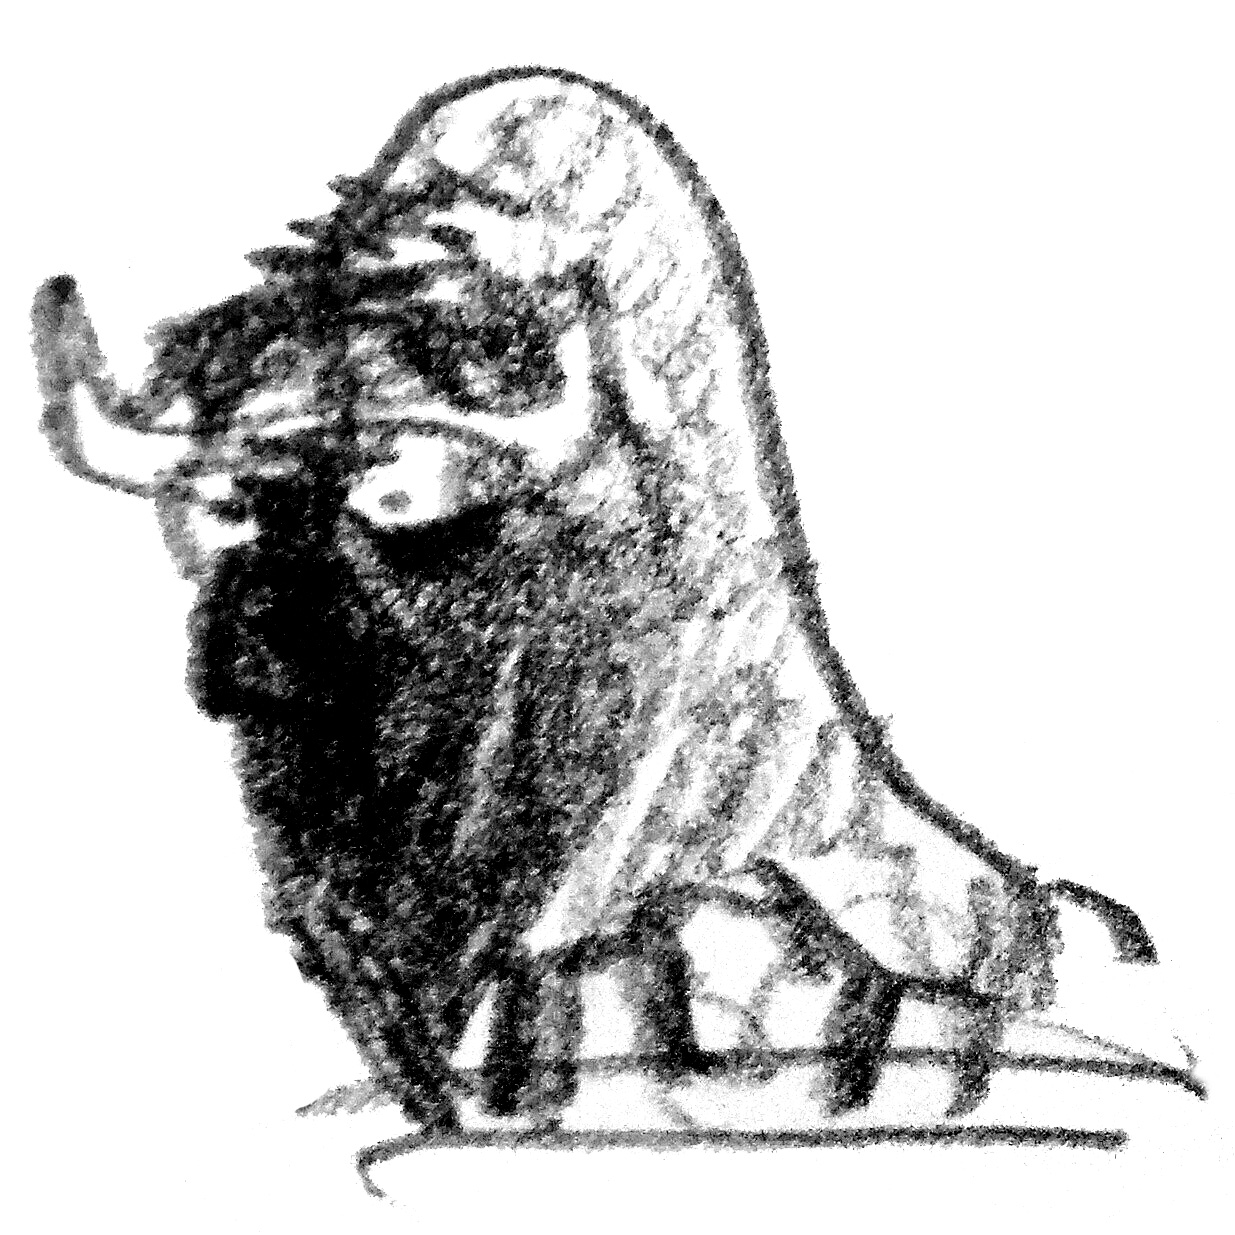
\includegraphics[height=1em]{bison/bison-qed.jpg}}}

\title{Hunting Acoustic Echoes for Auditory Scene Analysis}
\author{Diego DI CARLO}
\date{\today}

\begin{document}
\frontmatter{}


% % front matter / titelei
% recto: halftitlepage / schmutztitelseite, vortitel
\thispagestyle{empty}
{
    \begin{fullwidth}
        \centering
        \hphantom{.}
        \vfill
        {\Huge
            Security Arguments and\\
            Tool-based Design of Block Ciphers
        }
        \vfill
        \vfill
    \end{fullwidth}
}

\clearpage{}

% verso: frontispiece / frontiszipzseite, vakatseite
% dedication
\cleardoublepage{}

% recto: titlepage / titelblatt, innentitel
\thispagestyle{empty}
{
    \calccentering{\unitlength}
    \begin{adjustwidth*}{\unitlength}{-\unitlength}
        \raggedleft{}
        {\Huge\color{Burgundy}%
        Security Arguments and\\
        Tool-based Design of Block Ciphers}\\[\baselineskip]
        {\LARGE%
        Dissertation Thesis}\\[0.2\textheight]
        {\huge%
        Friedrich Wiemer}\\[\baselineskip]
        {\LARGE%
        16th~August 2019}
        \vfill
        \vfill
        {\large%
        Submitted in partial fulfillment of the requirements\\
        for the degree of Doktor der Naturwissenschaften\\[\baselineskip]% (Dr.\ rer.\ nat.)\\[\baselineskip]

        to the\\[\baselineskip]

        Faculty of Mathematics\\
        at Ruhr-Universität Bochum\\[2\baselineskip]
        %Vorgelegt zur Erlangung des\\
        %Doktorgrades der Naturwissenschaften\\
        %an der Fakultät der Mathematik\\
        %der Ruhr-Universität Bochum\\[2\baselineskip]

        \begin{minipage}{0.5\textwidth}
        \begin{tabular}{lr}
            1st\hspace{4pt} Reviewer & Prof.\ Dr. Gregor Leander\\
            2nd Reviewer & Prof.\ Dr.\; Alexander May
        \end{tabular}
        \end{minipage}
        \hspace*{36pt}
        %}\hspace*{-8pt}

        %\vspace{2\baselineskip}
        %Datum der Disputation: 13.\ Dezember 2019
        \vfill
        }
        \vspace*{\baselineskip}
    \end{adjustwidth*}
}

\clearpage{}

% verso: colophon / impressum
\thispagestyle{empty}
\hphantom{.}
\vfill

\section*{Imprint}

\textit{Security Arguments and Tool-based Design of Block Ciphers}\\
Copyright \textcopyright{} 2019 by \theauthor{}.\\
All rights reserved. Printed in Germany.\\
Published by the Ruhr-Universität Bochum, Bochum, Germany.

\section*{Colophon}

This thesis was typeset using \LaTeX{} and the \texttt{memoir} documentclass.
It is based on Aaron Turon's thesis \emph{Understanding and expressing scalable concurrency}\footnote{\url{https://people.mpi-sws.org/~turon/turon-thesis.pdf}}, itself a mixture of \texttt{classicthesis}\footnote{\url{https://bitbucket.org/amiede/classicthesis/}} by Andr\'e Miede and \texttt{tufte-latex}\footnote{\url{https://github.com/Tufte-LaTeX/tufte-latex}}, based on Edward Tufte's \emph{Beautiful Evidence}.\\[0.5\baselineskip]
%
The bibliography was processed by Biblatex.
All graphics and plots are made with PGF/Ti\emph{k}Z.\\[0.5\baselineskip]
%
The body text is set 10/14pt (long primer) on a 26pc measure.
The margin text is set 8/9pt (brevier) on a 12pc measure.
Matthew Carter's \textrm{Charter} acts as both the text and display typeface.
Monospaced text uses Jim Lyles's \texttt{Bitstream Vera Mono} (\enquote{Bera Mono}).

\clearpage{}

% recto: dedication or epigraph
\thispagestyle{empty}
\vphantom{.}
\vfill
{%
    \flushright{}
    \emph{If we knew what it was we were doing,\\
          it would not be called research, would it?}\\
    \hfill---Albert Einstein
}
\vfill
\vfill

% verso: blank
\clearpage{}

% front matter / titelei
% recto: halftitlepage / schmutztitelseite, vortitel
\thispagestyle{empty}
{
    \begin{fullwidth}
        \centering
        \hphantom{.}
        \vfill
        {\Huge
            Hunting Echoes\\
            for\\
            Auditory Scene Analysis
        }
        \vfill
        \vfill
    \end{fullwidth}
}

\clearpage{}

% verso: frontispiece / frontiszipzseite, vakatseite
% dedication
\cleardoublepage{}

% recto: titlepage / titelblatt, innentitel
\thispagestyle{empty}
{
    \calccentering{\unitlength}
    \begin{adjustwidth*}{\unitlength}{-\unitlength}
        \raggedleft{}
        {\Huge\color{Burgundy}%
        Hunting Echoes\\
        for Auditory Scene Analysis}\\[\baselineskip]
        {\LARGE%
        Dissertation Thesis}\\[0.2\textheight]
        {\huge%
        Diego \textsc{Di Carlo}}\\[\baselineskip]
        {\LARGE%
        \today}
        \vfill
        \vfill
        {\large%
        Submitted in partial fulfillment of the requirements\\
        for the degree of Doktor der Naturwissenschaften\\[\baselineskip]% (Dr.\ rer.\ nat.)\\[\baselineskip]

        to the\\[\baselineskip]

        Faculty of Mathematics\\
        at Ruhr-Universität Bochum\\[2\baselineskip]
        %Vorgelegt zur Erlangung des\\
        %Doktorgrades der Naturwissenschaften\\
        %an der Fakultät der Mathematik\\
        %der Ruhr-Universität Bochum\\[2\baselineskip]

        \begin{minipage}{0.5\textwidth}
        \begin{tabular}{lr}
            1st\hspace{4pt} Reviewer & Prof.\ Dr. Gregor Leander\\
            2nd Reviewer & Prof.\ Dr.\; Alexander May
        \end{tabular}
        \end{minipage}
        \hspace*{36pt}
        %}\hspace*{-8pt}

        %\vspace{2\baselineskip}
        %Datum der Disputation: 13.\ Dezember 2019
        \vfill
        }
        \vspace*{\baselineskip}
    \end{adjustwidth*}
}

\clearpage{}

% verso: colophon / impressum
\thispagestyle{empty}
\hphantom{.}
\vfill

\section*{Imprint}

\textit{Hunting Echoes for Audtory Scene Analysis}\\
Copyright \textcopyright{} 2020 by \theauthor{}.\\
All rights reserved. Printed in France.\\
Published by the Ruhr-Universität Bochum, Bochum, Germany.

\section*{Colophon}

This thesis was typeset using \LaTeX{} and the \texttt{memoir} documentclass.
It is based on Aaron Turon's thesis \emph{Understanding and expressing scalable concurrency}\footnote{\url{https://people.mpi-sws.org/~turon/turon-thesis.pdf}}, itself a mixture of \texttt{classicthesis}\footnote{\url{https://bitbucket.org/amiede/classicthesis/}} by Andr\'e Miede and \texttt{tufte-latex}\footnote{\url{https://github.com/Tufte-LaTeX/tufte-latex}}, based on Edward Tufte's \emph{Beautiful Evidence}.\\[0.5\baselineskip]
%
The bibliography was processed by Biblatex.
All graphics and plots are made with PGF/Ti\emph{k}Z.\\[0.5\baselineskip]
%
The body text is set 10/14pt (long primer) on a 26pc measure.
The margin text is set 8/9pt (brevier) on a 12pc measure.
Matthew Carter's \textrm{Charter} acts as both the text and display typeface.
Monospaced text uses Jim Lyles's \texttt{Bitstream Vera Mono} (\enquote{Bera Mono}).

\clearpage{}

% recto: dedication or epigraph
\thispagestyle{empty}
\vphantom{.}
\vfill
{%
    \flushright{}
    \emph{Pleasure to me is wonder—the unexplored, the unexpected, \\
    the thing that is hidden and the changeless thing\\
    that lurks behind superficial mutability.}\\
    \hfill--- Howard Phillips \textsc{Lovercraft}
}
\vfill
\vfill

% verso: blank
\clearpage{}


\chapter*{Abstract}\addcontentsline{toc}{chapter}{Abstract}

Audio\marginpar{
    \footnotesize
    \textbf{Keywords:}
    \\Acoustic echoes, acoustic echo retrieval, room impulse response estimation;
    audio scene analysis, room acoustics;
    audio source separation, room geometry estimation, spatial filtering, sound source localization;
    deep learning, continuous dictionary.
} scene analysis aims at retrieving useful information from microphone recordings.
Examples of these problems are sound source separation and sound source localization, where we are interested in estimating the content and location of multiple sources of sound in an environnement.
As humans, we perform these tasks without effort. However, for computers and robots, they are still open challenges.
One of the main limitations is that most available technologies solve audio scene analysis problems either ignoring how sound propagates in the environment or estimating it fully.

\mynewline
The central theme of this theses is acoustic echoes: the sound propagation elements bridging semantic and spatial information on sound sources.
Indeed, as repetitions of a source signal, their semantic contributions can be aggregated to enhance this signal.
Moreover, since they originate from an interaction with the environment, their paths can be backtracked and used to estimate the audio scene's geometry.
Based on these observations, recent echo-aware audio signal processing methods have been proposed.
However, two main questions arise: how to estimate acoustic echoes, and how to use their knowledge?

\mynewline
This thesis work aims at improving the current state-of-the-art for indoor audio signal processing along these two axes.
It also provides new methodologies and data to process acoustic echoes and surpass current approaches' limits.
To this end, in the first part, we present two approaches:
a novel approach based on the  continuous dictionary framework which does not rely on parameter tuning or peak picking techniques;
a deep learning model estimating the time differences of arrival of the first prominent echoes using physically-motivated regularizers.
Furthermore, we present a novel, fully annotated dataset specifically designed for acoustic echo retrieval and echo-aware applications, paving the way for future echo-aware research.

\mynewline
The second part of this thesis focuses on extending existing methods in audio scene analysis to their echo-aware forms.
The Multichannel NMF framework for audio source separation, the SRP-PHAT localization method, and the MVDR beamformer for speech enhancement are extended to in their echo-aware versions.
These applications show how a simple echo model can lead to a boost in performance.

\newthought{This thesis} highlights the difficulty of exploiting acoustic echoes to improve indoor audio processing.
As a first attempt to lay unified analytical and methodological foundations for these problems, it is hoped to serve as a starting point for promising new research in this field.
% Finally, we want to underline the difficulty related to the tasks of estimating and exploiting acoustic echoes to improve indoor audio processing.
% Therefore, this thesis consists only of a first attempting work that lays analytical foundations on how to model such problems, and it can serve as a starting point for new exciting directions.
\blankpage{}
\chapter*{Résumé en français}\addcontentsline{toc}{chapter}{Résumé en français}

% This summary presents in French an overview of the work addressed in this thesis.

% The audio scene analysis topic covers many different tasks that aim to retrieve useful information from microphone recordings.
% Examples of these problems are sound source separation and sound source localization, where we are interested in estimating a speaker's content and position.
% As humans, we perform these tasks without effort: imagine someone calling us from the other side of the room. Your typical reaction would probably turn your attention towards or even go to him/her.
% However, for computers and robots, using audio signal processing techniques, are still open challenges.

% Sounds convey semantic information (what your friends said), temporal and spatial (when he said it, where he said it).
% We can model these contributions using signals describing the sound content and room impulse response, accounting for its propagation in the space. Some audio processing methods focus on the former, ignoring or roughly describing the latter due to the challenging task of estimating it.
% Room Impulse responses embed all the elements of sound propagation, such as echoes, diffuse reflection, and reverberation.

% The central theme of this theses are acoustic echoes. These elements of sound propagation create a bridge between semantic and spatial information of sound sources. As they are repetitions and copies of the source sound, we can weigh more the target sound by integrating their contribution than other noise sources.
% As these reflections are originated by the interaction of the source sound with the environment, thanks to their arrival time, we can retrace back their paths and, thus, reconstruct the geometry of the audio scene's geometry.
% Based on these observations, audio signal processing methods started to account for these sound propagation elements to solve the audio scene analysis problem.
% Two are the main questions that arise:
% how we estimated acoustic echoes, and how we use their knowledge?

% This thesis work aims at improving the current state-of-the-art for indoor audio signal processing along these two axes.
% In particular, it provides new methodologies and data to process acoustic echoes and surpass current approaches' limits.
% Second, it extends previous classical methods for audio scene analysis in their echo-aware form.
% These two claims are elaborated in the two main parts of the thesis, which follow after an introductory one, as summarized below.

% First, we provide some preliminary definitions of the role of audio signal processing and list some fundamental problems which will be considered throughout the thesis, namely, acoustic echo retrieval, audio source separation, sound source localization, room geometry estimation.

% The~\cref{ch:acoustics} will build a first important bridge: from acoustics to audio signal processing. It first defines sound, how it propagates in the environment, and how this origins echoes.

% In~\cref{ch:processing},  we move from physic to digital signal processing where the echoes are modeled as elements of filters, called Room Impulse Responses (RIRs), operating on the source signal.
% Because processing in the native time domain is complicated, we present the Fourier representation, which facilitates both the exposure of the methods and the implementation of the algorithms.
% This chapter closes the first introductory part.

% In this second part of the thesis, we are interested in estimating early acoustic echoes from microphone recordings. Based on the models and the definition described in the first part, this part includes first a general overview of echo retrieval methods followed by the presentation of two works published at international conferences and a dataset that is about to be released.

% First, in chapter~\cref{ch:estimation}, we provide the reader with knowledge of the state-of-the-art about Acoustic Echo Retrieval, namely, on how to estimate acoustic echoes properties. After presenting the problem and the literature is review according to typical taxonomy used in signal processing. In order to provide a complete look at Acoustic Echo Retrieval, some datasets and evaluation metrics recurring in the literature and used in the following chapter are presented.

% In this second part of the thesis, we are interested in estimating early acoustic echoes from microphone recordings.
% Based on the models and the definition described in the first part, this part includes first a general overview of echo retrieval methods followed by the presentation of two works published at international conferences and a dataset that is about to be released.

% First, in chapter~\cref{ch:estimation}, we provide the reader with knowledge of the state-of-the-art about Acoustic Echo Retrieval, namely, on how to estimate acoustic echoes properties. After presenting the problem and the literature is review according to typical taxonomy used in signal processing. In order to provide a complete look at Acoustic Echo Retrieval, some datasets and evaluation metrics recurring in the literature and used in the following chapter are presented.

% The following three chapters presented three works we conducted on Acoustic Echo Estimation.

% \cref{ch:blaster} presents a novel approach for estimating echoes from a stereophonic recording of an unknown sound source such as speech.  In contrast with existing methods, it is built on the recent continuous dictionary framework and does not rely on parameter tuning or peak picking techniques.
% The method's accuracy and robustness are assessed on challenging simulated setups with varying noise and reverberation levels and are compared to two state-of-the-art methods. Experimental evaluation on synthetic data shows that comparable or slightly worse recovery rates are observed for recovering seven echoes or more. Instead, better results are obtained for a fewer number of echoes, and the off-grid nature of the approach yields generally smaller estimation errors.
% Nevertheless, this is promising since the practical advantage of knowing the timing few echoes per channel will be demonstrated in the last part of the thesis.

% In~\cref{ch:lantern}, we deploy deep learning techniques to estimate acoustic echoes properties. To the best of our knowledge, this is one of the first examples in these directions. The proposed method shares some common grounds with deep learning techniques already applied in sound source localization. We will present three different architecture which addresses the acoustic echo estimation problem with increasing order of complexity: estimating the time of arrival of the direct path and the first prominent echos; perform this estimation in a more robust way; and, finally, extend it to an increasing number of echoes.

% Finally, to conclude this second part, in~\cref{ch:dechorate}, we describe a dataset we collected, specifically designed for acoustic echo estimation. This dataset features measured multichannel room impulse response (RIRs), including annotations of early echoes and 3D positions of microphones and real and image sources under different wall configurations in a cuboid room. These data provide a new tool for benchmarking recent methods in \textit{echo-aware} audio signal processing and software utilities to easily access, manipulate, and visualize the data.

% The third and last part of the thesis concern the audio processing applications where the knowledge of early echoes may improve the performance over standard methods.
% For the occasion, we assume that echoes properties are available a priori and build our prior knowledge.
% The structure of this part follows the format of the previous one.

% An introductory chapter gathers the standard definitions and introduces the current state-of-the-art approaches for indoor audio processing under the same umbrella.
% We consider three fundamental problems: audio source separation, sound source localization, spatial filtering, and room geometry estimation.
% These problems are presented in turn with the related literature review, highlighting the current challenges.
% These particular problems will be the protagonist of the following three chapters, presented in their echo-aware form.

% In~\cref{ch:separake}, echoes are used for boosting the performance of classical Audio Source Separation methods and results from a collaboration with other colleagues, published in an international conference.
% In particular, we propose a physical interpretation of the echoes, namely, image microphones, which allow understanding better how the algorithms benefit from their knowledge.
% Our investigation considers two variants of the multichannel nonnegative matrix factorization source separation framework: one that uses only magnitudes of the transfer functions and uses the phases.
% The results show that the proposed approach beats its vanilla variant by using only a few echoes and echoes enable separation where it was considered unaffordable.

% \cref{ch:mirage} addresses the problem of audio source localization in the context of strong acoustic echoes. Using the model of image microphones presented in the previous chapter, we show that these interfering contributions can be used to change the classic way source localization performed.
% In particular, we show that in a simple scenario involving two microphones close to a reflective surface and one source, the proposed approach is able to estimate both azimuthal and elevation angles, impossible task assuming an ideal propagation, as classical approaches do.
% These results were merged into a publication, published in an international conference.
% Furthermore, the investigation is then extended to microphone arrays featuring multiple sensors and to real-world data, provided by a collaboration with the research team of Honda.

% The ~\cref{ch:dechorateapp} presents two echo-aware applications that can benefit from the dataset \dEchorate, presented in~\cref{ch:dechorate}. We exemplify the utilization of these data considering two possible audio scene analysis problems: echo-aware spatial filtering and room geometry estimation.
% In order to validate the data and show their potential, well-known state-of-the-art algorithms are used. Therefore, for each of the applications, the considered methods are contextualized and summarized.
% Numerical results confirm the value of this dataset for the audio signal processing community. The dataset and these methods will be released publicly so that external contributors will be invited to use them for developing more robust audio processing methods.

% The last chapter (\cref{ch:conclusing}) recapitulates the main results presented in this manuscript and the perspectives related to this work.
% Among them, we show how few acoustic echoes can be estimated from the only observation of microphone recordings featuring reverberant speech using either model derived from the physics of the sound propagation and deep learning models trained on acoustic simulators.
% Moreover, we demonstrate the strengths of including the knowledge of acoustic echoes in audio processing methods.
% For the aspect related to the evaluation of echo-aware methods in a real-world scenario, we advocate that freely-available benchmarking datasets are currently missing in the literature. Therefore, in the spirit of open research, we build a new dataset which will soon be released. These data are accompanied by accurate annotation and algorithmic tools for echo-aware research covering much application for audio scene analysis.

% Finally, we want to underline the difficulty related to the task of estimating and exploiting acoustic echoes to improve indoor audio processing. This thesis, therefore, consists only in a first attempting work that lays analytical foundations on how to model such problems.
% Like all the first investigations, a lot can be improved, and we hope it can serve as a starting point for new interesting, and challenging researches.
\blankpage{}

\chapter*{Acknowledgements}\addcontentsline{toc}{chapter}{Acknowledgements}

Block ciphers form, without doubt, the backbone of today's encrypted communication and are thus justifiably the workhorses of cryptography.
While efficiency of modern designs improved ever since the development of the DES and AES, the case with the corresponding security arguments differs.
The thesis at hand aims at two main points, both in the direction of improving security analysis of block ciphers.

Part~I studies a new notion for the better understanding of a special type of cryptanalysis and proposes a new block cipher instance.
This instance comes with a tight bound on any differential, to the best of our knowledge the first such block cipher.

Part~II turns to automated methods in design and analysis of block ciphers.
Our main contribution here is an algorithm to propagate subspaces through encryption rounds, together with two applications: an algorithmic security argument against a new type of cryptanalysis and an idea towards the automation of key recovery attacks.
\addcontentsline{toc}{chapter}{Acknowledgments}
\cleardoublepage{}

\tableofcontents*\addcontentsline{toc}{chapter}{Contents}
\clearpage{}

% \listofalgorithms\addcontentsline{toc}{chapter}{List of Algorithms}
% %\clearpage{}
% \vspace{\baselineskip}

\listoffigures*\addcontentsline{toc}{chapter}{List of Figures}
\vspace{\baselineskip}
\clearpage{}

\listoftables*\addcontentsline{toc}{chapter}{List of Tables}
\clearpage{}

\mainmatter{}
\begin{fullwidth}
\part{Prologue}
\end{fullwidth}

\cleardoublepage{}

\itodo{Can we use \bison/'s argument (regarding differential cryptanalysis) for a maximal unbalanced Feistel network?}
\itodo{Can we improve \cref{st:lem:2} so that we do not have to compute the span of the union over all basis vectors?}

% \chapter{Introduction}
\openepigraph{Nanos gigantum humeris insidentes.}{Bernard of Chartres}
\openepigraph{If I have seen further, it is by standing on the shoulders of giants.}{Isaac Newton}

Cryptography is by now used for more than 30 centuries.
While in ancient times encrypting messages seemed more like an art, our understanding of the security needs and techniques greatly evolved during the last decades.
Likewise, the field of cryptology has greatly grown and research specialised in many different aspects, mainly dividable in the underlying techniques of symmetric and asymmetric cryptography.
The prime difference between these two is that for symmetric ciphers both encryption and decryption needs the same secret key, while in asymmetric ciphers the so-called public key is used for encryption (and does not have to be kept secret) and only the secret key allows decryption.

Especially such fascinating recent developments of techniques like secure multiparty computation or fully homomorphic encryption have the chance to significantly impact our privacy needs of today's digital world.
While these techniques mainly rely on asymmetric cryptography, symmetric cryptography is still the technique of choice when it comes to plain old encryption of messages.

\newthought{Block ciphers}\hspace{1.5em} are today's workhorse of symmetric encryption
\marginpar{%
    \footnotesize
    For a more precise and technical introduction to block ciphers and their analysis see the following \cref{ch:prelim}, in particular \cref{sec:prelim:bc,sec:prelim:cryptanalysis}.
}
-- and thus responsible for the majority of all encrypted data.
Opposed to public key primitives, which security properties can often be reduced to cryptographic or complexity theoretic hardness assumptions and thus often come with a provable security notion, our trust in symmetric primitives is mainly built from extensive cryptanalysis.
Informally, a secure block cipher is thus one that withstood cryptanalysis long enough and resists all known attacks; from a more theoretical point of view we require a secure block cipher to be interchangeably usable for a random permutation, \ie/ the block cipher should not be distinguishable from a family of random permutations.

To ease this analysis, simplifying the concrete design of a primitive is a fruitful ansatz.
A very common approach is to design the cipher as an iteration of a simple, in itself insecure, round function.
The overall security of the block cipher is then built piecewise over several rounds of encryption.
To further ease the analysis of the round function, it is often built independently of the encryption (round) keys.
The key-material is instead introduced in between the rounds, often by XOR-ing it into the cipher's state.
Such constructions are known as key-alternating ciphers, whereof the best known instance is the \AES/.\footnote{%
    Some people call it the \enquote{king of bock ciphers}.
}
Compared to \enquote{older} block cipher designs, such as that of the \DES/ or \blowfish/,\footnote{%
    \DES/' Feistel structure is arguable more complex than that of comparable modern Feistel ciphers as \eg/ \sm4/, the Chinese symmetric encryption standard.
    \blowfish/ uses key-dependent S-boxes, which make it considerable harder to reason about its precise resistance against known attacks.
} this kind of, very simple and elegant, design allows us to throughly understand its properties and build confidence in its security.
After 20 years of cryptanalysis, we can justifiably say that the \AES/ is today's best understood design and (even more important) remains a \emph{secure} block cipher.

Albeit one might think the existence of standards like the \AES/ renders the design of new block ciphers needless, plenty of new designs where proposed since the publication of the \AES/.

\newthoughtpar{Incentives for new Cipher Designs}
It is a legitimate concern to ask why we still keep designing new ciphers all the time.
\emph{Lightweight cryptography} is the latest most important trend in symmetric cryptography, at least since the publication of the block cipher \present/,\footnote{%
    Since its publication in 2007 and at the time of writing, the most cited cryptographic paper, according to \href{https://www.sec.cs.tu-bs.de/~konrieck/topnotch/crypto_top100.html}{Konrad~Rieck}~\citeonly{WEB:Rieck19} (visited 09--06--2019).
} with its current peak in NIST's (the National Institute of Standards and Technology) \LWC/ competition.
The main reason for lightweight cryptographic designs is the assumption that existing standards, \eg/ the \AES/, are too costly for heavily constrained devices such as medical implants, RFID tags, or sensors for the \iot/.
Another interesting direction is the design of special purpose ciphers,\footnote{%
    Two examples are \lowmc/, see Albrecht et~al., \enquote{Ciphers for MPC and FHE}, and \rasta/, see Dobraunig et~al., \enquote{\rasta/: A cipher with low ANDdepth and few ANDs per bit}.
} \ie/ ciphers which are built for the use in one specific application and are thus specifically tailored to the corresponding requirements.

An obvious advantage is the gain in efficiency for such specialised designs.\footnote{%
    However it might often be that the \enquote{\AES/ is lightweight enough}, see \href{https://blog.teserakt.io/2019/06/03/cryptography-in-industrial-embedded-systems-our-experience-of-the-needs-and-constraints/}{Aumasson et~al.}~\citeonly{WEB:Teserakt19} (visited 09--06--2019).
}
The main advantage is actually a different one.
Vigorously optimising block cipher designs to be as efficient as possible leads to designs with sometimes very narrow security margins -- or them even being broken.
Such designs at the border of security sometimes enable weaknesses to occur, for which \enquote{normal} designs are just \enquote{too secure}.
A prime example is the \printcipher/ which was later broken by structural attacks with the discovery of invariant subspace attacks.
However, these designs provide us with the valuable insight of what is important for the security of a block cipher.

Designing new block ciphers thus enables us to broaden our understanding of which structures provide what kind of security.
Eventually this process of designing and analysing new block ciphers will lead to very few standardised encryption algorithms that are then recommended to use in real world applications.

\section{Open Problems in Block Cipher Design}

Efficiency of symmetric ciphers have been significantly improved further and further over the past years, in particular within the trend of lightweight cryptography.
However, when it comes to arguing about the security of ciphers, the progress is rather limited and the arguments basically did not get easier nor stronger since the development of the \AES/.
It might thus be worth shifting the focus to improving security arguments for new designs rather than (incrementally) their efficiency.

Maybe the top goal of cryptanalysis should be to fully understand and thoroughly exploit every cryptanalytic attack that we can mount on block ciphers.

\newthoughtpar{Full Understanding of Cryptanalytic Attacks}
Being a noble goal, the often computational infeasible kind of cryptanalytical attacks on cryptographic designs renders it seemingly impossible to achieve.

In particular even with so well-studied attacks as differential and linear cryptanalysis, effects (differentials and linear hulls) occur which we do not fully understand, even for ciphers like the \AES/.
Giving tight security bounds in such a case is inherently difficult.
Thus, two problems, exemplary for differential and linear cryptanalysis, are
\marginpar{%
    \footnotesize
    \vspace{\baselineskip}
    \vspace*{-7\baselineskip}
    See \cref{sec:prelim:dc} for a detailed explanation of differential cryptanalysis and the problems that appear when trying to bound the differential probability.

    \Cref{sec:prelim:lc} discusses linear cryptanalysis and the respective problems with the linear hull.
}
\begin{problem}[Differentials]\label{prob:differentials}
    Given a cipher $E$, compute a (tight) bound on the probability that a differential through $E$ holds.
\end{problem}
and
\begin{problem}[Linear Hulls]\label{prob:linear_hulls}
    Given a cipher $E$, compute a (tight) bound on the correlation for a linear hull to approximate $E$.
\end{problem}

\newthoughtpar{Security Arguments for Block Ciphers}
Two very distinct flavours of security arguments for cipher designs are provable security arguments (asymptotic and concrete security) on the one hand, and resistance to practical attacks on the other hand.
For example, the generic (or idealised) security of key-alternating ciphers was studied in recent years and one can prove that for breaking such an $r$-round construction one has to make roughly $2^{\frac{r}{r+1}n}$ oracle queries.

While this bound can be proven to be tight for key-alternating ciphers, it is unsatisfactory for two reasons.
First, one might hope to get better security bounds with different constructions and second one might hope to lower the requirements used in the security proof.
A similar goal to the above is thus to find new generic constructions that allow very strong security proofs.

\begin{problem}[Block Cipher Constructions]\label{prob:cipher_constructions}
    Find new secure constructions for block ciphers.
\end{problem}
\marginpar{%
    \footnotesize
    \vspace*{-3\baselineskip}
    We recall the most common constructions for block ciphers in \cref{sec:prelim:bcc} and discuss results on their security in \cref{sec:prelim:concrete-sec}.
}

For the more practical part of cryptanalysis, and apart from the first two problems, it might also well be the case that new attacks are discovered.
In such a case, all previously published ciphers that remained secure have to be evaluated against this new attack.
To ease this process, easily verifiable arguments for the resistance against a new technique are very helpful.

\begin{problem}[Provable Resistance]\label{prob:prove_res_attack}
    Given an attack for block ciphers, find provable properties to show the resistance against this attack.
\end{problem}
\marginpar{%
    \footnotesize
    \vspace*{-3\baselineskip}
    The common heuristic argument for resistance against differential and linear cryptanalysis is discussed in \cref{sec:prelim:dc,sec:prelim:lc,sec:prelim:practical-sec}.
}

\newthoughtpar{Automatisation of Design and Cryptanalysis}
Having easy to check theorems for the resistance of a cipher against some type of attack is already a good basis.
It might still be connected with a huge amount of (tedious) work, to check the security of many block ciphers.
For example, in the first round of the \LWC/ competition, 56 candidate designs were accepted (out of 57 submissions).
In case we found a new attack for block ciphers, we would have to check each of these candidates if and how well this attack is applicable.

It is thus very helpful if tedious and repetitive analysis tasks can be automated.
This does not only save time we can spend on more productive research, but also reduces the probability of making errors during the analysis.
So, similar to \cref{prob:prove_res_attack}:
\begin{problem}[Algorithmic Resistance]\label{prob:alg_res_attack}
    Given an attack for block ciphers, find an algorithmic way to show the resistance against this attack.
\end{problem}

Attacks on symmetric ciphers are often based on two parts, see \cref{sec:prelim:cryptanalysis} for more details.
First, the cryptanalyst finds some non random behaviour that can be turned into a distinguisher for some rounds of the cipher.
For a lot of attacks there are methods that find such distinguishers automatically.
Second, this distinguisher is extended by a key guessing part to turn the distinguishing attack into a key recovery attack, where the key guesses are verified by the distinguisher.
This second part involves a lot of manual bit-fiddling and precise details of the cipher under scrutiny -- and is thus prone to errors.
\begin{problem}[Automate Key Recovery]\label{prob:key_rec}
    Given a distinguisher $D$ for $r$ rounds of a cipher $E$, algorithmically turn this distinguisher into a key recovery attack over a maximal number of $r+s$ rounds for $E$.
\end{problem}

But not only during the analysis of cryptographic primitives, also when initially designing them, automated methods can be of great help.
For example when specific parameters have to be optimised, a computer-aided process is virtually indispensable for the exploration of the design space.
\begin{problem}[Optimise Building Block]\label{prob:optimise_bb}
    Given a set of constraints for a building block and some cost metric, find an optimal instance for this building block regarding that metric.
\end{problem}

In the next section, we first briefly sketch the outline of the thesis and then summarise the contributions in the context of the above problems.

\section{Outline and Contributions}

The remainder of the thesis is structured as follows.
In the following \cref{ch:prelim} we discuss preliminary notions, constructions, and analysis techniques for block ciphers.
The technical parts of the thesis are then split in two.

In \textsc{Security Arguments for Block Ciphers}, we discuss an analysis tool\footnote{%
    The \DLCTl/ by \citeauthor{EC:BDKW19}.
} published at \textsc{EuroCrypt}'19 and its connection to established notions for (vectorial) Boolean functions, see \cref{ch:act} and~\cite{EPRINT:CanKolWie19}.
The following \cref{ch:bison} describes our instances \bison/ and \wisent/ of the \WSNs/ construction; it is based on~\cite{EC:CLLNW19}.

The next part, \textsc{Automated Methods in Design and Analysis}, is split in three \cref{ch:slp,ch:st,ch:key_rec}.
We first discuss heuristic methods for optimising implementations of matrix multiplications in hardware, see also~\cite{ToSC:KLSW17}.
Then we turn our attention to cryptanalysis and study an algorithmic way to propagate truncated differentials and subspace trails through \SPN/ constructions.
For the discussed algorithm, we propose two applications: bounding the length of any subspace trails, and approaching the automatisation of key recovery attacks (the first is based on~\cite{ToSC:LeaTezWie18}).

Finally, \cref{ch:conclusion} concludes the thesis.

In particular, the respective contributions are the following.

\subsection{Security Arguments for Block Ciphers and Understanding of Attacks}
This part consists of contributions to the understanding of differential-linear cryptanalysis and our instances of the \WSNs/ construction.

\newthoughtpar{Autocorrelation Tables and Differential-Linear Cryptanalysis}
\textcite{EC:BDKW19} proposed a new analysis tool for differential-linear cryptanalysis which allows them to give a more precise estimation of several differential-linear distinguishers published so far.
Following the same pattern as similar tools for differential, linear and boomerang attacks, they coin it \DLCT/.
However, the authors did not analyse the \DLCT/ from a theoretical point in detail.

We continue the analysis at this point and provide further insights on the \DLCT/.
In particular, we show that this table coincides with the already known \ACT/ -- highlighting an interesting new connection between resistance to differential-linear attacks and the autocorrelation of vectorial Boolean functions.
Additionally, we discuss further properties of the autocorrelation in the case of vectorial Boolean functions.
Our analysis contributes to the understanding of resisting differential-linear attacks, see \crefName{prob:prove_res_attack}.

\newthoughtpar{\bison/ -- Instantiating the WSN construction}
The \WSN/ construction by \textcite{AC:Tessaro15} is an alternative construction for block ciphers.
By proving the security of his construction, \citeauthor{AC:Tessaro15} provides a solution to \crefName{prob:cipher_constructions}.
In this regard, his work just comes with one drawback: there is no instance of this construction yet.
But when building such an instance, one fundamentally has to instantiate the building blocks modeled as ideal functionalities.
Furthermore, such a practical instance has to be scrutinised from a symmetric cryptanalysis perspective and has to provide security against known attacks.
Thus, without an instance and further analysis, the underlying constructing remains of no avail.

In~\cite{EC:CLLNW19}, we close this gap and suggest an instance of the \WSN/ construction, completing \citeauthor{AC:Tessaro15}'s solution to \cref{prob:cipher_constructions}.
For this instance, we first derive some (rather trivial but nevertheless important) design rationales.
Based on these properties every secure instance has to fulfill, we conduct further cryptanalysis.
As a result of this analysis, we give a tight bound for any non-trivial differential through such an instance, thus solving \crefName{prob:differentials} for this case.
Note that, to the best of our knowledge, no other secure cipher is known, for which we are able to solve this problem.

In the remainder of the chapter, we then define our instance more precisely -- that is, we give a concrete specification for an instance fulfilling our generic restrictions.
We call this instance \bison/\footnote{%
    \bison/ is a Bent whItened Swap-Or-Not cipher.
}, as it is based on bent Boolean functions.
Afterwards, we extend the cryptanalysis of \bison/ to other attacks and discuss performance figures.
The main drawback from an implementers perspective of \bison/ (apart from being impractically slow) is that we can only instantiate odd block length versions of it.
For an actual use in hard- or software, we would however strongly prefer even block lengths.

We thus extend the work from~\cite{EC:CLLNW19} and give a second instance, for even block lengths, of the \WSN/ construction, which follows our initial analysis.
Due to its close connection to \bison/, we name this instance \wisent/.
Here, too, we extend the analysis to other common attacks and give performance figures.

\subsection{Automated Methods in Design and Analysis}%
This part consists of contributions to the optimisation of XOR counts, algorithmic security arguments for subspace trails and an automatisation approach for key recovery strategies.

\newthoughtpar{Heuristics for XOR counts}
Recently, finding optimal linear layers in block ciphers, an instance of \crefName{prob:optimise_bb}, attracted a lot of interest.
Here, the building block we are looking for is a matrix $M$, where the multiplication by $M$ corresponds to the application of the linear layer.
Typically, this matrix should exhibit some special properties, \eg/ being \MDS/, due to security reasons.
The metric under which we want to find an optimal matrix is then the number of gates (hardware) or instructions (software) needed in an implementation.

As the design space usually is too large for exhaustive search, we have to apply other methods.
For example, proofs for the minimal costs of multiplications by single elements were given by some authors, \eg/ \textcite{C:BeiKraLea16,EC:Kolsch19}; a typical optimisation strategy for a complete matrix would then be to choose the matrix elements from the cheapest elements possible.
This can be seen as a local optimisation strategy.

In~\cite{ToSC:KLSW17}, we observe that optimising the matrix implementation globally, that is reusing intermediate results from one element multiplication for another, can save a lot of resources.
Further we observe that this problem of finding an optimal implementation is known as finding the shortest linear straight line program for this implementation.
Moreover, a whole branch of research exists on solving this problem.
As finding short linear straight line programs is NP-hard, several heuristic approaches were proposed in the literature.
In the remainder of this chapter, we discuss and evaluate the effectiveness of these heuristics.
Eventually we are able to improve all known current best implementations with little effort.

While this contributes towards solving \cref{prob:optimise_bb} for this case, it seems rather impossible to ultimately solve this problem, as we discuss at the end of this chapter.

\newthoughtpar{Propagating Truncated Differentials}
While standard differential cryptanalysis is quite well understood, this is not the same case for its variants.
For example when it comes to truncated differentials, no generic security argument for the resistance against this attack is known.
Additionally, the new notion of subspace trails, see~\cite{ToSC:GraRecRon16}, which is related to truncated differentials, allowed to discover new properties of the \AES/, \eg/~\citeonly{EC:GraRecRon17,C:BDKRS18} (after 20 years of cryptanalysis).
It is thus important to improve our understanding of these attacks.

In~\cite{ToSC:LeaTezWie18} we contribute towards this goal.
We first show the exact relation between subspace trails and truncated differentials for their probability-one versions.
Afterwards, we develop an algorithm to propagate a given subspace trail through an \SPN/ round function.
We further give properties and algorithmic ways to show an (\SPN/) cipher's resistance, thus partly solving \cref{prob:prove_res_attack,prob:alg_res_attack} for this attack.
Finally we apply our algorithms to a list of \SPN/ ciphers and give precise bounds on the longest subspace trails for each of them.

\newthoughtpar{Key Recovery}
As a second application of our propagation algorithm for truncated differentials, we turn our focus to \crefName{prob:key_rec}.
We observe that extending a differential distinguisher is closely related to subspace trails and truncated differentials of probability one.
Based on this finding, we discuss ideas how to exploit this relation in order to automate the construction of key recovery attacks.

\section{Publications}

During the course of my doctoral studies, I worked on several projects which are not all covered in the remainder of this thesis.
In particular, these are the following.

\newthoughtpar{Conference Publications}
\begin{itemize}
    \item[] \fullfullcite{EC:CLLNW19}, see \cref{ch:bison}.
            %Because \bison/ can only be instantiated with odd block length, we here also give a second instance of the underlying construction: \wisent/.
            %This instance is for the even block length case and basically inherits almost the same security bounds as \bison/.
\end{itemize}

\newthoughtpar{Journal Publications}
\begin{itemize}
    \item[] \fullfullcite{ToSC:KraLeaWie17}.
    \item[] \fullfullcite{ToSC:KLSW17}, see \cref{ch:slp}.
    \item[] \fullfullcite{ToSC:LeaTezWie18}, see \cref{ch:st}.
\end{itemize}

\newthoughtpar{Other Publications, Preprints and Submitted Work}
\begin{itemize}
    \item[] \fullfullcite{EPRINT:CanKolWie19}, see \cref{ch:act}.
\end{itemize}
To these five papers, all authors contributed equally.
We merged the last paper with the results from~\citeonly{ARXIV:LLLQ19}:
\begin{itemize}
    \item[] \fullfullcite{CKLLLQW19}.
\end{itemize}
I am also involved in the design of the NIST \LWC/ submission \spook/:
\begin{itemize}
    \item[] \fullfullcite{LWC:Spook}.
\end{itemize}
I contributed to the cryptanalysis of the underlying primitives \clyde/ and \shadow/, in particular to the choice of round constants, the analysis of subspace trails, and division properties.

Further, I contributed to the development of \sage/ by authoring the following tickets.
Additionally I also reviewed tickets not listed here.
\begin{itemize}
    \setlength\itemsep{0em}
    \item[] \fullfullcite{SAGE:14549}
    \item[] \fullfullcite{SAGE:21252}
    \item[] \fullfullcite{SAGE:22453}
    \item[] \fullfullcite{SAGE:22986}
    \item[] \fullfullcite{SAGE:22988}
    \item[] \fullfullcite{SAGE:23830}
    \item[] \fullfullcite{SAGE:24566}
    \item[] \fullfullcite{SAGE:24819}
    \item[] \fullfullcite{SAGE:24872}
    \item[] \fullfullcite{SAGE:25516}
    \item[] \fullfullcite{SAGE:25633}
    \item[] \fullfullcite{SAGE:25708}
    \item[] \fullfullcite{SAGE:25733}
    \item[] \fullfullcite{SAGE:25735}
    \item[] \fullfullcite{SAGE:25739}
    \item[] \fullfullcite{SAGE:25744}
    \item[] \fullfullcite{SAGE:25765}
    \item[] \fullfullcite{SAGE:25766}
    \item[] \fullfullcite{SAGE:26009}
    \item[] \fullfullcite{SAGE:28001}
\end{itemize}

Before we proceed to the technical parts, we now recall basic techniques for the design and analysis of block ciphers.

% \chapter{The Art and Science of Block Cipher Design}\label{ch:prelim}
\openepigraph{%
    Nicht Kunst und Wissenschaft allein,\\Geduld will bei dem Werke sein.%\\[0.25\baselineskip]
    %Not Art and Science serve alone;\\Patience must in the work be shown
}{Johann Wolfgang von Goethe}
\openepigraph{During human progress, every science is evolved out of its corresponding art.}{Herbert Spencer}

\vspace*{-\baselineskip}
\newthought{Shannon's}\hspace{1.5em} \enquote{A Mathematical Theory of Cryptography}~\citeonly{shannon45} is commonly referred to as the founding stone of modern cryptography.
While modern cryptography knows several kinds of encryption and authentication schemes, the trinity of symmetric cryptography consists of encryption schemes, hash functions and message authentication codes.
This thesis focuses on the design and analysis of symmetric encryption schemes, in particular block ciphers.
In the following sections we give an overview of constructions and techniques used for these tasks.
While doing so, we discuss some issues in our actual understanding of the subject and where the work of a practising cryptographer might still be declared an art.
At best, these issues can be answered by developing new tools and techniques to advance the science of cryptography.

Before coming to the technical parts, let us quickly recall some basic notations and linear algebra.
\section{Basics and Notations}
By $\F_2 = \set{0,1}$ we denote the finite field with two elements, by $\F_{2^k}$ the extension field with $2^k$ elements, often also denoted as $\mathrm{GF}(2^k)$, and by $\F_2^n$ the $n$ dimensional vector space over $\F_2$.
We denote the addition in a finite field, an extension field and vector space by $+$; in the last case it corresponds to the component-wise addition in the underlying field.
The addition is also commonly referred to as \enquote{XOR}.
For the (scalar) multiplication in $\F_2$, $\F_{2^n}$ and $\F_2^n$, as well as the canonical \emph{inner product} in $\F_2^n$ we write $\iprod{x}{y} \coloneqq \sum_i x_i y_i$ (for $x,y \in \F_2^n$), and it is clear from the context whether the multiplication or inner product is meant.
The \emph{span} of a set $U \subseteq \F_2^n$
\begin{equation*}
    \Span{U} \coloneqq \set{\sum_{u \in U} \lambda_u u \given \lambda_i \in \F_2}
\end{equation*}
denotes the minimal subspace of $\F_2^n$ that contains all linear combinations of elements in $U$.
Given a subspace $U \subseteq \F_2^n$, we denote a \emph{basis} of $U$ by $\Basis{U}$, that is a minimal subset of $U$ such that it's span is equal to $U$:
\begin{equation*}
    U = \Span{\Basis{U}}\;.
\end{equation*}
Note that in general a basis is not unique.
The canonical basis vectors are $e_i$, \ie/ $e_i$ has exactly one component equal to one at position~$i$.
The \emph{dimension} of a subspace is the size of its basis, denoted $\dim{U} = \abs{\Basis{U}}$.
Given another subspace $V \subseteq \F_2^n$ with trivial intersection $U \cap V = \set{0}$, we denote the \emph{direct sum} by
\begin{equation*}
    U \oplus V \coloneqq \set{u + v \given u \in U\ \text{and}\ v \in V} \subseteq \F_2^n
\end{equation*}
and the \emph{direct product} by
\begin{equation*}
    U \times V \coloneqq \set{(u, v) \given u \in U\ \text{and}\ v \in V}\;.
\end{equation*}
If $U \oplus V = \F_2^n$, we say $V = U^c$ is a \emph{complement} of $U$.
If further for all $u \in U$
\begin{equation*}
    \iprod{u}{v} = 0 \quad \forall v \in V\;,
\end{equation*}
$V = U^\bot$ is the \emph{orthogonal complement}.
It is also referred to as perpendicular complement or \emph{dual space}.

The two following properties of orthogonal complements are well known.
\begin{lemma}[Orthogonal Complement of direct products]
    The orthogonal complement of a direct product is the direct product of its orthogonal complements:
    \begin{equation*}
        \parens{V_1 \times \cdots \times V_n}^\perp = V_1^\perp \times \cdots \times V_n^\perp.
    \end{equation*}
\end{lemma}
\begin{proof}
    We give the proof for $n = 2$.
    It can be extended to general $n$ by induction.
    Let $V_1$, $V_2 \subseteq \F_2^n$ be subspaces.
    \begin{itemize}
        \item[$\subseteq$]
            Let $a \in \parens{V_1 \times V_2}^\perp$.
            $\forall v = (v_1, v_2) \in V_1 \times V_2 : \iprod{a}{v} = \iprod{a_1}{v_1} + \iprod{a_2}{v_2} = 0$.
            As this holds for every $v$ (in particular also for every $v = (0, v_2)$ and $v = (v_1, 0)$), both summands have to be constant zero.
            It follows that $a_1 \in V_1^\perp$, $a_2 \in V_2^\perp$ and thus $a = (a_1, a_2) \in V_1^\perp \times V_2^\perp$.
        \item[$\supseteq$]
            Let $a = (a_1, a_2) \in V_1^\perp \times V_2^\perp$.
            $\forall (v_1, v_2) \in V_1 \times V_2 : \iprod{\parens{\begin{smallmatrix}a_1 \\ a_2\end{smallmatrix}}}{\parens{\begin{smallmatrix}v_1 \\ v_2\end{smallmatrix}}} = \iprod{a_1}{v_1} + \iprod{a_2}{v_2} = 0$.
            Thus $a = (a_1, a_2) \in \parens{V_1 \times V_2}^\perp$.
    \end{itemize}
\end{proof}

\begin{lemma}[Orthogonal Complement of subsets]\label{st:lem:subset_complements}
    Let $U \subseteq V$ be a subspace.
    The orthogonal complement of $V$ is a subset of the orthogonal complement of~$U$.
    Formally:
    \begin{equation*}
        U \subseteq V \Rightarrow V^\perp \subseteq U^\perp\;.
    \end{equation*}
\end{lemma}
\begin{proof}
    From the definition of the orthogonal complement we have $\forall a \in V^\perp : \forall v \in V : \iprod{a}{v} = 0$.
    As $U$ is a subset of $V$ this also holds in particular for all the elements in $U$: $\Rightarrow \forall a \in V^\perp : \forall u \in U : \iprod{a}{u} = 0$.
    Which finally implies that $V^\perp \subseteq U^\perp$.
\end{proof}

We denote the set of $\F_2$-linear functions $L : \F_2^n \to \F_2^m$ ($\F_2$-homo\-mor\-phisms) as
\begin{equation*}
    \mathrm{Hom}_{\F_2}(\F_2^n, \F_2^m) \coloneqq \set{L : \F_2^n \to \F_2^m \given L\ \text{is linear}}\;.
\end{equation*}
By fixing a basis there exists a natural isomorphism to $m \times n$ matrices, $\mathrm{Hom}_{\F_2}(\F_2^n, \F_2^m) \cong \mathrm{Mat}_{m,n}(\F_2)$ and we can thus identify every linear function~$L$ by a corresponding matrix $T_L$, called the \emph{matrix representation} of $L$.
The \emph{kernel} of $L$ (or $T_L$) is the set of all elements mapped to zero:
\begin{equation*}
    \Ker{L} \coloneqq \set{x \in \F_2^n \given L(x) = 0} \subseteq \F_2^n
\end{equation*}
the \emph{image} of $L$ (or $T_L$) is
\begin{equation*}
    \Im{L} \coloneqq \set{L(x) \given x \in \F_2^n} \subseteq \F_2^m\;.
\end{equation*}

We denote the set of functions on $\F_2^n$ as $\func/_n$, the set of permutations on $\F_2^n$ as $\perm/_n$, and the set of Boolean functions, \ie/ all $f : \F_2^n \to \F_2$, as $\boolfunc/_n$.
The subset of linear Boolean functions, $\mathrm{Hom}_{\F_2}(\F_2^n, \F_2) \subset \boolfunc/_n$, forms a subspace with the direct sum of functions $(f + g)(x) \coloneqq f(x) + g(x)$.
Further, the natural isomorphism for linear Boolean functions to~$\F_2^n$ is
\begin{gather*}
    \Phi : \F_2^n \to (\F_2^n \to \F_2) \\
    \Phi(\alpha) \coloneqq x \mapsto \iprod{\alpha}{x}\;.
\end{gather*}
Affine linear Boolean functions are of the form $x \mapsto \iprod{\alpha}{x} + 1$ for $\alpha \in \F_2^n$.
Any linear or affine Boolean function which is not constant is balanced, \ie/ $f(x)$ equals zero and one equally often.
This implies the fundamental fact
\begin{equation}\label{eqn:sum-fact}
    \sum_{x \in \F_2^n} \parens{-1}^{\iprod{\alpha}{x}} = \begin{cases*}
        2^n & if $\alpha = 0$ \\
        0   & else
    \end{cases*}\;.
\end{equation}
The \emph{adjoint} function $L^\top$ of $L$ is the function, such that
\begin{equation}\label{eqn:adjoint}
    \forall x,y \in \F_2^n : \iprod{x}{L(y)} = \iprod{L^\top(x)}{y}
\end{equation}
The matrix representation of $L^\top$ corresponds to the transposed matrix representation of $L$.
For further background on Boolean functions, we refer to \cref{sec:prelim:bf}.

A fundamental theorem is the following.
\begin{theorem}[Rank-Nullity Theorem]\label{thm:rank-nullity}
    Given a linear function $L : \F_2^n \to \F_2^m$, where $n \geqslant m$.
    Then
    \begin{equation*}
        \dim{\Im{L}} + \dim{\Ker{L}} = n\;.
    \end{equation*}
\end{theorem}
\begin{proof}
    Denote $\Basis{\Ker{L}} = B = \set{u_1, \ldots, u_m}$.
    We can extend this basis to form a basis of the whole $\F_2^n = \Span{A \cup B}$, with $A = \set{v_1, \ldots, v_{n-m}}$.
    Note that we can write the image of $L$ as
    \begin{align*}
        \Im{L} &= \Span{L(A \cup B)} \\
               &= \Span{L(u_1), \ldots, L(u_m), L(v_1), \ldots, L(v_{n-m})} \\
               &= \Span{L(v_1), \ldots, L(v_{n-m})} \\
               &= \Span{L(A)}\;,
    \end{align*}
    where $A$ forms a basis of $\Im{L}$, as we show next.

    By contradiction.
    Assume there are $\lambda_i \in \F_2$ not all zero, such that
    \begin{align*}
        0 &= \sum_{i=1}^m \lambda_i L(v_i) \\
        \intertext{and, as $L$ is linear}
          &= L\parens{\sum_{i=1}^m \lambda_i v_i}\;,
    \end{align*}
    which implies that $\sum_{i=1}^m \lambda_i v_i$ is actually in the kernel of $L$.
    This contradicts the assumption of $A \cup B$ being a basis of $\F_2^n$.

    Finally
    \begin{equation*}
        \dim{\Im{L}} + \dim{\Ker{L}} = \abs{A} + \abs{B} = n-m + m = n
    \end{equation*}
    concludes the proof.
\end{proof}
The name of the theorem stems from the fact that the dimension of the image is called \emph{rank} and the dimension of the kernel \emph{nullity}.

Up to isomorphisms, every extension field with $2^k$ elements is equal to the univariate polynomial ring over $\F_2$ modulo an irreducible polynomial~$q(x)$ of degree $k$: $\F_{2^k} \cong \F_2[x]/q(x)$.
In favour of a more compact notation, we stick to the common habit and write a polynomial as its coefficient vector interpreted as a hexadecimal number, \ie/ $q(x) = x^4 + x + 1$ corresponds to $\mathtt{0x13}$.

It is well known that we can represent the elements in a finite field with characteristic two as vectors with coefficients in $\F_2$.
More precisely, by fixing a basis there exists a vector space isomorphism $\Phi: \F_{2^k} \to \F_2^k$.
Every multiplication by an element $\alpha \in \F_{2^k}$ can then be described by a left-multiplication with a matrix $T_{\alpha} \in \F_2^{k \times k}$ as shown in \cref{fig:slps:vs_iso} (and is thus a linear operation).
For an element~$\alpha$,~$T_{\alpha}$ is usually called its \emph{multiplication matrix}.
Note that $T_\alpha$ depends on the chosen basis.
\marginpar{%
    \centering
    \footnotesize
    \begin{tikzpicture}[node distance=2cm]
        \node (ul) {$\mathbb{F}_{2^k}$};
        \node (ur) [right of=ul] {$\mathbb{F}_{2^k}$};
        \node (ll) [below of=ul] {$\mathbb{F}_2^k$};
        \node (lr) [below of=ur] {$\mathbb{F}_2^k$};

        \path [line, thin] (ul) edge node[above] {$\cdot \alpha$} (ur);
        \path [line, thin] (ul) edge node[left] {$\Phi$} (ll);
        \path [line, thin] (ll) edge node[below] {$T_{\alpha}$} (lr);
        \path [line, thin] (lr) edge node[right] {$\Phi^{-1}$} (ur);
    \end{tikzpicture}
    \captionof{figure}{Multiplication using a vector space isomorphism}
    \label{fig:slps:vs_iso}
}

Given an $n \times n$ matrix $M = (\alpha_{i,j})$ with $\alpha_{i,j} \in \F_{2^k}$ for $1 \leq i,j \leq n$, we define its \emph{binary representation} as the corresponding binary $nk \times nk$ matrix
\begin{equation*}
    \binarymatrix{M} \coloneqq (T_{\alpha_{i,j}}) \subseteq \GL{k}^{n \times n} \subseteq (\F_2^{k \times k})^{n \times n} \cong \F_2^{nk \times nk}\;.
\end{equation*}
Here, $\mathrm{GL}(k, \F_2)$ denotes the general linear group, that is the group of invertible matrices over $\F_2$ of dimension $k \times k$.

Given a matrix $M$ and a vector $u$, the \emph{Hamming weights} $\mathrm{hw}(M)$ and~$\mathrm{hw}(u)$ are defined as the number of nonzero entries in $M$ and $u$, respectively.
In the case of a binary vector $v \in \F_2^{nk}$, we define the \emph{$k$-bit word Hamming weight} as $\mathrm{hw}_k(v) \coloneqq \mathrm{hw}(v')$, where $v' \in (\F_2^k)^n$ is the vector that has been constructed by partitioning $v$ into groups of $k$ bits.

Finally, some notational conventions:
We denote uniformly random sampling from a finite set by $\in_R$, that is $x \in_R M$ denotes that $x$ is drawn uniformly at random from the set~$M$.
Given a vector $x \in \F_2^n$, we normally index a single element at position $i$ as $x_i$.
However, to avoid ambiguity, we might also denote the $i$-th element as $x[i]$.
If $x$ is split into parts, we denote a \enquote{slice} of $x$ as $x[i:j] \coloneqq (x_i, x_{i+1}, \ldots, x_j)$ for $i \leqslant j$.

\section{Pseudorandom Permutations and Block ciphers}\label{sec:prelim:bc}

First and foremost, we assume Kerckhoffs' century-old principle~\cite[p.~12, 2nd condition]{kerckhoffs83}, \ie/ that the description of any encryption scheme (and of all its parts) is publicly available.

On the way to build a secure encryption system, several questions arise.
In this section we strive to answer these in a top-down approach.
The first and most important question is: how do we define security?
There are multiple approaches to answer this initial problem, which we briefly sketch here.
For the first part of this section, we orientate ourself by the asymptotic security notion, discussed in detail \eg/ by \textcite{katzlindell}.
To relate the security properties of particular block cipher constructions at the end of this section, we recall the concrete security notion, see~\cite{FOCS:BDJR97}.
Such an answer basically consists of three parts: what we want to achieve (the notion of security), what an adversary can do (her capabilities), and how she wants to break our security notion (her goal).
We summarise these properties in our attacker model.

Apart from this fundamental security discussion, we then shortly discuss ways of turning a block cipher into a secure encryption scheme.
In particular, we cover how the security functionality is abstractly modeled by a pseudorandom permutation, which is then in practice instantiated as a block cipher.
Such a pseudorandom permutation or block cipher is then turned into a secure encryption scheme using a mode of operation and a padding scheme.

Afterwards we turn to block ciphers in more detail and discuss typical constructions and inner building blocks for them.
Eventually we recall concrete security statements for the most common block cipher construction.

\subsection{Generic Security for Generic Constructions}
Our ultimate goal for a secure encryption is to hide information from an adversary, \ie/ providing \emph{confidentiality}.\footnote{%
    The other two most important security goals are \emph{integrity} (the data is unmodified) and \emph{message authentication} (verifying the identity of the sender), which can be achieved by message authentication codes.
    However, for the remainder of the thesis, we focus on confidentiality.
}
We thus want to design a secure encryption scheme for which an adversary is not capable of deducing any information from the plaintext.

\newthoughtpar{Attacker Model}
We assume probabilistic polynomial-time (and thus computationally bounded) adversaries.
Typically three \emph{attack scenarios} are discussed which describe the capabilities of such an attacker.
\begin{description}
    \item[\KPA/] The adversary learns some pairs of plain- and ciphertexts, encrypted under the same key.
    \item[\CPA/] The adversary \begin{inparaenum}[1)]
            \item gets oracle access to the encryption function,
            \item outputs two challenge plaintexts $m_0$, $m_1$, and learns the encryption $c^\prime$ of $m_b$ for a uniformly random chosen bit $b$.
        \end{inparaenum}
    \item[\CCA/] The adversary \begin{inparaenum}[1)]
            \item gets oracle access to the encryption and decryption function,
            \item outputs two challenge plaintexts $m_0$, $m_1$, learns the encryption $c^\prime$ of $m_b$, for a uniformly random chosen bit $b$,
            \item is not allowed to query the decryption of $c^\prime$.
        \end{inparaenum}
\end{description}
Clearly, \KPA/ is the weakest and \CCA/ the strongest scenario.

When dealing with asymptotic security, the standard goal of an attacker in the above scenarios is to distinguish between two messages, \ie/ guessing the bit~$b$ correctly.
However, for an practical attack on an encryption scheme, other goals might also be of interest.
Standard goals of an attacker are thus
\begin{description}
    \item[Distinguishing] The adversary has to distinguish two encryptions.
    \item[Plaintext Recovery] The adversary has to decrypt a fresh ciphertext.
    \item[Key Recovery] The adversary has to recover the secret key used by the oracle.
\end{description}
In general, security against a distinguishing attack is the most generic goal and thus the most difficult to achieve.
This is intuitively clear, as an attacker that successfully recovers a key or a plaintext can easily be turned into an attacker that distinguishes ciphertexts (\ie/ by recovering the key, decrypting the ciphertext or directly recovering the plaintext and then distinguish based on this plaintext).
If not specified, we thus assume the adversary's goal to be a distinguishing attack.
We later discuss the connection between different goals in the specific case of symmetric cryptanalysis, but keep the discussion general for this introduction.

In order to prove asymptotic security, the standard technique are reductionistic, game-based proofs.
For these, we define a security game that an adversary has to win with a high enough probability, in order to break the security claim of the scheme.
One then shows under a suitable hardness assumption that such an attacker can be transformed into an attacker on the underlying hardness assumption.
In the context of symmetric cryptography, we do not base our proofs on hardness assumptions, but give \emph{concrete} bounds on the adversary's advantage.
Thus we refrain from defining all these notions in full rigor; provable security is anyway not the topic of the remaining thesis.

Let us now turn to the constructive part and discuss approaches to achieve a secure encryption system.

\newthoughtpar{Constructions: Pseudorandom Permutations and Block Ciphers}
The first encryption scheme that can be proven secure is the \emph{\OTP/}.
It was developed even before World War II and used then, during the Cold War, and most probable is still in use today.
The encryption is simply $\mathrm{OTP}_k : m \mapsto k + m$, where key and message are both in $\F_2^n$, while the crucial fact for the \OTP/'s security is based on the \emph{one time} use of the key $k$.
In particular, for every message, we need a fresh key sampled uniformly at random.

The \OTP/ comes with one prime advantage and one prime disadvantage.
Using a uniformly random key only once enables us to prove the \OTP/ secure in a information-theoretic sense -- that is an even stronger security notion that we have discussed and remains secure even if we allow computationally \emph{un}bounded adversaries.
So it provides the best security we can hope for, see also~\cite[Section~10]{Shannon49} for a generalised treatment.
However, as the downside of this \emph{perfect security}, we need uniformly random keys of the same length as our message which we want to encrypt.
In some sense this just shifts the problem of keeping the message confidential to the problem of exchanging a key of this length in a secure manner.
While it might be possible for some parties (\ie/ on a state level), to solve this problem, it is not practical for almost anyone.

Note that encrypting more than one message with the same key, directly breaks the security of the \OTP/ (in a \KPA/ scenario).
Nevertheless, this blinding technique is basically at the heart of every encryption.

As this first encryption scheme is not practically useful in most cases, we are interested in alternative constructions.
We cut the discussion short and mimic the \OTP/ encryption, but with the goal of achieving a secure system that can use a fixed, small key to encrypt many messages.
This is achievable, as we are aiming for security against computationally \emph{bounded} adversaries.

A candidate for such a secure (probabilistic) encryption scheme is the following:
\begin{equation}\label{eqn:enc-prp}
        E_k(x) \coloneqq (r, F_k(r) + x)\;.
\end{equation}
Here, $r$ is used to randomise the encryption as otherwise we cannot achieve \CPA/-security.
Any deterministic encryption scheme is \CPA/-insecure:
An attacker can simply query the encryption of its challenge messages and distinguish the challenge ciphertext based on these two encryptions.

The remaining, yet unspecified, part is~$F_k$, and we want to take a more detailed look at what properties it has to exhibit, so that our scheme is secure.

The intuition we follow here is that the output of~$F_k$, for any fixed key~$k$, should look random and is (against our computationally bounded adversary) indistinguishable from a true uniformly random output.
This is captured in the notion of a pseudorandom permutation, that is: an efficient, (length-preserving), keyed permutation which is computationally indistinguishable from a random permutation.
Here, being efficient implies a polynomial-time algorithm for evaluating the permutation.
Length-preserving is assumed for simplicity and denotes a permutation of~$\F_2^n$, where the key is also an element of~$\F_2^n$.\footnote{%
    We later discuss an instance of a pseudorandom permutation with a different key length than~$n$ -- which in practice often occurs, but for the moment we stay with the simplified notation (as the generalisation is trivial anyway).
}
The notion of computationally indistinguishability captures the intuition that any probabilistic polynomial-time attacker's success probability is negligible, \ie/ smaller than $1/\mathrm{poly}(n)$.
More formally we end up with the following definition.
\begin{definition}[Pseudorandom Permutation]\label{def:prp}
    Given a family of functions~$F$ on $\F_2^n$.
    We call $F_k$ a \emph{\PRP/} if
    \begin{itemize}
        \item $F_k$ is a permutation of~$\F_2^n$,
        \item there exists polynomial-time algorithms evaluating $F_k$ and $F_k^{-1}$, and finally
        \item for all probabilistic polynomial-time distinguishers $D$ the following probability bound holds:
              \begin{equation}\label{eqn:prp-def}
                  \abs{\Prob\bracket{D^{F_k}(1^n) = 1} - \Prob\bracket{D^{f}(1^n) = 1}} \leqslant \negl{n}\;,
              \end{equation}
              where $\negl{n} < \frac{1}{\mathrm{poly}(n)}$ for all polynomials in $n$.
              The probability space is over the uniform choice of the key~$k$, the permutation $f \in_R \perm/_n$ and the randomness of $D$.
    \end{itemize}
    We call $n$ the \emph{security parameter}, which is, for length-preserving functions, equal to the \emph{block size} and \emph{key size}.
\end{definition}
The above \cref{eqn:prp-def} has to be interpreted in the following way.
The distinguisher $D$ has oracle access to either $F_k$ or to a random permutation $f$ -- here, oracle access implies that she can query the oracle for inputs to the corresponding functions and learns as a response the output of the function.
$D$ has then to distinguish which oracle (the pseudorandom or the true random permutation) she has access to and answers this by outputting an answer bit $b$.
This bit encodes the pseudorandom case as $b=1$ and the true random case as $b=0$.
The distinguishers \emph{advantage} is then the statistical distance between these two cases, \ie/
\begin{equation*}
    \mathrm{Adv}_D^\mathrm{PRP}(F_k, f) \coloneqq \abs{\Prob\bracket{D^{F_k}(1^n) = 1} - \Prob\bracket{D^{f}(1^n) = 1}}\;.
\end{equation*}
If $D$ is not able to distinguish the pseudorandom permutation from a true random one, this distance is negligible and thus \emph{computational indistinguishable}.
The $1^n$ input specifies the all-one-vector $(1, \ldots, 1) \in \F_2^n$, a technical detail to link the security parameter with the requested \enquote{polynomial in the input length}-runtime of~$D$.

Note that a computationally unbounded adversary can always violate the computational indistinguishable notion, see the margin note.
\marginpar{%
    \footnotesize
    \vspace*{-4\baselineskip}
    \textbf{An unbounded adversary breaks\\computational indistinguishability}\\[2pt]
    The following distinguisher $D$ has a non negligible advantage.

    \begin{itemize}
        \item Get access to an oracle $\mathcal{O}$
        \item Query $\mathcal{O}$ for every possible input, \ie/ compute the vector\\
              $v = (\mathcal{O}(i))_{i \in \F_2^n}$.
        \item For every possible $k \in \F_2^n$, compare \\
              $v \stackrel{?}{=} (F_k(i))_{i \in \F_2^n}$.
        \item If they are equal, output $b = 1$.
        \item If none of the vectors are equal, output $b = 0$.
    \end{itemize}

    Clearly, the probability to output the correct bit in the case of $\mathcal{O} = F_k$ is one.
    Moreover, D outputs the wrong bit in the case of $\mathcal{O} = f$, if the uniformly chosen random permutation $f = F_k$.
    This occurs with probability less than $1/(2^n-1)$ and hence is negligible.
    $D$'s overall advantage is thus close to one.
}
This problem does not occur when analysing the concrete security of a cipher, as the adversary's advantage is then bounded by her resources.

The above security definition can be extended, by allowing the distinguisher to access the inverse permutation, too.
This leads to the notion of a strong pseudorandom permutation:
\begin{definition}[Strong Pseudorandom Permutation]\label{def:strong-prp}
    A function-family $F$ on $\F_2^n$ is a \emph{strong \PRPl/} if $F$ is a \PRP/ and for any $k \in \F_2^n$ and for all probabilistic polynomial-time distinguishers $D$ the following probability bound holds:
    \begin{equation*}
        \abs{\Prob\bracket{D^{F_k,F_k^{-1}}(1^n) = 1} - \Prob\bracket{D^{f,f^{-1}}(1^n) = 1}} \leqslant \negl{n}\;.
    \end{equation*}
    The probability space is over the uniform choice of the key $k$, the permutation $f \in_R \perm/_n$ and the randomness of~$D$.
\end{definition}

However, returning to our construction, we do not need a strong \PRP/ to show the following.
Under the assumption that $F$ is a \PRP/, the construction in \cref{eqn:enc-prp} is \CPA/-secure.
As we have not formally defined \CPA/-security, we leave out the proof.
The interested reader can find the rigorous definitions, constructions and security proofs in~\cite{katzlindell}.

On our way to a secure encryption scheme, we are now left with building a \PRP/.
Block ciphers are designed to yield exactly this, a secure instance of a (strong)~\PRP/ (where we now allow the key to have a different length).
\begin{definition}[Block Cipher]\label{def:bc}
    A \emph{Block Cipher} is a family of permutations $E$ of the~$\F_2^n$.
    Any instance of $E$ is indexed by the \emph{master key} $k \in \F_2^m$.
    We call $n$ the \emph{block size} and $m$ the \emph{key size} of $E$.
    Furthermore we require that (for every $k$) $E_k$ (and its inverse $D_k = E_k^{-1}$) is efficiently computable, \ie/ there exists a probabilistic polynomial-time algorithm evaluating $E_k$.
\end{definition}
While standard block cipher designs fix one block size $n$, a technical oddity is that among others polynomial time looses its meaning.
For the efficient computable aspect, we simply ignore this and just require \enquote{an efficient implementation}.
However, for the asymptotic security argument, this fixed $n$ is problematic, too.
Namely in order that a block cipher is secure, we would typically request it to be a (strong)~\PRP/.
Above, we have already mentioned the problems with a standard rigorous security proof: it would require proving the \PRP/ property under a (weak) complexity theoretic hardness assumption (as it is done for most asymmetric designs).
Now, fixing any block size $n$ directly renders the asymptotic argument of bounding the advantage by some negligible term useless.
In contrast to encryption schemes or similar, for block ciphers it is often not possible to give a generic construction for any block size $n$.
This problem is typically circumvented by bounding the adversary's advantage with the concrete resources she spends, see also the discussion in \cref{sec:prelim:concrete-sec}, in particular \cref{def:concrete-prp}.

Nevertheless, proofs in this concrete setting still retain the problem that they base on idealised building blocks.
Instead of doing such a proof, we typically \enquote{just assume} that any \emph{practical} block cipher instance is secure, \ie/ a (strong) \PRP/.
The main reason for this approach is owed to efficiency requirements and the fact that designs asymptotically proven to be secure are often several magnitudes slower than modern block ciphers.
Certainly, this missing last brick in the security proof should not be interpreted wrongly.
Years of public scrutiny support our assumption that a specific block cipher actually yields a \PRP/.
Comparing such a thoroughly understood design with asymmetric schemes that rely on \eg/ the complex Gap-Diffie-Hellman assumption,\footnote{%
    For Gap-Diffie-Hellman we assume the Decisional-Diffie-Hellman problem (given $g$, $g^a$, $g^b$, and $g^c$, decide if $c=ab$ for a group generator $g$ and integers $a$, $b$ and $c$) to be easy and the Computational-Diffie-Hellman problem (given $g$, $g^a$, $g^b$, compute $g^{ab}$ for a group generator $g$ and integers $a$ and $b$) to be hard.
}
we should be much more confident in the security of the block cipher.
Additionally to the used hardness assumption, a block cipher also typically corresponds to one fixed instance for any parameter set, while an asymmetric scheme might change the parameters for every key pair.
This is the case \eg/ in RSA, where every key pair has to use a different modulus (otherwise the encryption is directly broken), and is in some sense even worse for elliptic curve-based systems.
Choosing efficient and secure elliptic curves is a highly non-trivial task -- and examples as the \texttt{Dual\_EC\_DRBG} incident\footnote{%
    See the Snowden leaks, in particular NSA's \enquote{Bullrun} program.
} confirm that it is possible to easily hide backdoors in such parameters, whereas no such way to hide backdoors for symmetric schemes are publicly known.

As our encryption scheme in \cref{eqn:enc-prp}, and analogously any block cipher, only encrypts single $n$-bit blocks of data, we typically need a \emph{mode of operation} for $E$, such that we can encrypt data of arbitrary length.
In the next section, we discuss these modes together with padding schemes, completing our treatment of generic constructions for symmetric encryption schemes.

\newthoughtpar{Modes of Operation}
Actually, the scheme from \cref{eqn:enc-prp} can already be seen as a mode of operation, which turns a \PRP/ into a fixed-length \CPA/-secure encryption function.
However, as just mentioned, in practice we need to encrypt multiple blocks of data.
A mode of operation then serves as a sort of protocol, describing how these multiple blocks can be encrypted.
It is then important to show the security guarantees of such a mode, typically under the assumption that the used block cipher is a \PRP/.

Given several blocks of a plaintext message $m_1, m_2, \ldots \in \F_2^n$ and a block cipher $E : \F_2^n \times \F_2^m \to \F_2^n$.
We recall three standard modes of operation, which encrypt the message as follows, see~\cref{fig:modes} for a graphical representation.
%\marginpar{%
%    \centering
%    \vspace*{-7em}
%    \begin{tikzpicture}
%        \node (Ek_in) {$m_i$};
%        \node (Ek) [below=2em of Ek_in,draw,rectangle,thick,rounded corners,minimum width=1cm,minimum height=1cm] {$E_k$};
%        \node (Ek_out)[below=2em of Ek] {$c_i$};
%        \path[line] (Ek_in) edge (Ek);
%        \path[line] (Ek) edge (Ek_out);
%    \end{tikzpicture}
%    \captionof{figure}{ECB Mode of Operation}\label{fig:modes-ecb}
%}
\begin{description}
    \item[\ECB/] Deterministically encrypts every block independently:
                 \begin{equation*}
                     c_i = E_k(m_i)\;.
                 \end{equation*}
                 Recall that any deterministic encryption does not provide \CPA/-security.
                 This mode has thus a more educational purpose on \enquote{how to \emph{not} encrypt several blocks}.
    \item[\CBC/] Chooses a random initial value $\mathrm{IV} = c_0 \in_R \F_2^n$.
                 The encryption adds the previous ciphertext to the next plaintext before encrypting it:
                 \begin{equation*}
                     c_i = E_k(m_i + c_{i-1})\;,
                 \end{equation*}
                 and the $\mathrm{IV} = c_0$ is sent as first ciphertext block.
    \item[\CTR/] Chooses a random counter $\mathrm{ctr} \in_R \F_2^n$.
                 The block cipher is then used in a streaming mode, where the counter is encrypted under the key and the produced output is added as a kind of key-stream to the plaintext.
                 For the next block, the counter is increased, thus $\mathrm{ctr}+i$ (where the addition is done in $\mathbb{Z}/2^n\mathbb{Z}$) is used to encrypt the $i$-th block:
                 \begin{equation*}
                     c_i = m_i + E_k(\mathrm{ctr}+i)\;.
                 \end{equation*}
                 A nice property of the \CTR/ mode is that it is embarrassingly parallel and computing errors in the encryption function only affect the corresponding message block (in contrast to the \CBC/ mode, where errors propagate to all consecutive blocks).
\end{description}
\marginpar{%
    \centering
    \footnotesize
    \vspace*{-40\baselineskip}
    \begin{tikzpicture}
        \node (Ek_in) {$m_i$};
        \node (Ek) [below=2em of Ek_in,draw,rectangle,thick,rounded corners,minimum width=7.5mm,minimum height=7.5mm] {$E_k$};
        \node (Ek_out)[below=2em of Ek] {$c_i$};
        \path[line] (Ek_in) edge (Ek);
        \path[line] (Ek) edge (Ek_out);
    \end{tikzpicture}
    \captionof{subfigure}{ECB}\label{fig:modes-ecb}
    \vspace*{2em}
    \begin{tikzpicture}
        \node (Ek_in_xor)[XOR,scale=1.2] {};
        \node (p) [above=2em of Ek_in_xor] {$m_i$};
        \node (iv) [left=2em of Ek_in_xor] {$c_{i-1}$};
        \node (Ek) [below=2em of Ek_in_xor,draw,rectangle,thick,rounded corners,minimum width=7.5mm,minimum height=7.5mm] {$E_k$};
        \node (Ek_out)[below=2em of Ek] {$c_i$};
        \path[line] (p) edge (Ek_in_xor);
        \path[line] (iv) edge (Ek_in_xor);
        \path[line] (Ek_in_xor) edge (Ek);
        \path[line] (Ek) edge (Ek_out);
        \path[line] (Ek.south) -- +(0,-5pt) -- +(15pt,-5pt) -- +(15pt,42pt) -- +(+30pt,42pt);
    \end{tikzpicture}
    \captionof{subfigure}{CBC}\label{fig:modes-cbc}
    \vspace*{2em}
    \begin{tikzpicture}
        \node (Ek_in) {$\mathrm{ctr}+i$};
        \node (Ek) [below=2em of Ek_in,draw,rectangle,thick,rounded corners,minimum width=7.5mm,minimum height=7.5mm] {$E_k$};
        \node (xor)[below=2em of Ek,XOR,scale=1.2] {};
        \node [left=7.5mm of xor] (m) {$m_i$};
        \node [right=7.5mm of xor] (c) {$c_i$};
        \path[line] (Ek_in) edge (Ek);
        \path[line] (Ek) edge (xor);
        \path[line] (m) edge (xor);
        \path[line] (xor) edge (c);
    \end{tikzpicture}
    \captionof{subfigure}{CTR}\label{fig:modes-ctr}
    \captionof{figure}[Modes of Operation]{Modes of Operation}\label{fig:modes}
}
%\marginpar{%
%    \centering
%    \vspace*{-10em}
%    \begin{tikzpicture}
%        \node (Ek_in) {$\mathrm{ctr}+i$};
%        \node (Ek) [below=2em of Ek_in,draw,rectangle,thick,rounded corners,minimum width=1cm,minimum height=1cm] {$E_k$};
%        \node (xor)[below=2em of Ek,XOR,scale=1.2] {};
%        \node [left=7.5mm of xor] (m) {$m_i$};
%        \node [right=7.5mm of xor] (c) {$c_i$};
%        \path[line] (Ek_in) edge (Ek);
%        \path[line] (Ek) edge (xor);
%        \path[line] (m) edge (xor);
%        \path[line] (xor) edge (c);
%    \end{tikzpicture}
%    \captionof{figure}{CTR Mode of Operation}\label{fig:modes-ctr}
%}
As just mentioned, \cref{eqn:enc-prp} can be seen as a fixed-length mode of operation; it is actually almost equal to the \CTR/ mode.
Besides the above mentioned modes, there are also other modes of operation which be used to build other symmetric primitives.
In particular, to turn a block cipher into a hash function the Davies-Meyer mode (proven secure in~\cite{C:BlaRogShr02}) can be used.
For a message authentication code \citeauthor{C:BelKilRog94} proved the CBC-MAC to be secure, see~\cite{C:BelKilRog94}.
More advanced modes are those that provide not only confidentiality, but also authentication.
These are known as authenticated encryption~(AE) or authenticated encryption with associated data~(AEAD).
As we normally want to provide a \CCA/-secure encryption scheme, such authentication is needed.
Hence the NIST \LWC/ competition's objective is to standardise such an AEAD scheme.

These manifold applications have lead to the fact that block ciphers are today's best understood primitives in the area of symmetric cryptography.
In particular the \AES/~\citeonly{FIPS:AES} has been scrutinised by cryptanalysts ever since its development in 1998~\cite{CARDIS:DaeRij98} without any significant security threat discovered for the full cipher (see \eg/~\citeonly{AES:Gilbert00,FSE:FKLSSWW00,C:BirKhoNik09,AC:BirKho09,AC:DunKelSha10,EC:DerFouJea13,ToSC:GraRecRon16,EC:GraRecRon17,AC:RonBarHel17}).

Before turning our attention to actually designing block ciphers, we want to cover one last part which is needed for the design of an encryption scheme: padding.
As the mode of operation allows us to encrypt messages of arbitrary length, it might well be the case that the message to be encrypted has not a length that is a multiple of the block cipher's block length.
Padding is then used to expand the last message block to the block length.
A very simple variant is the following bit-padding.
Given a message with $\ell$ blocks, where the last block $m_\ell$ is of length $r \leqslant n$.
We then extend $m_\ell$ by the string $10^k$, where $k = n-r-1$, if $r < n$, or $k = n-1$ in the case $r=n$.
Note that the last case actually result in a new message block $m_{\ell+1} = 10 \ldots 0$ and thus in a worst-case ciphertext expansion of $n$~bits.

An alternative to a padding scheme which does not expand the ciphertext is the so called ciphertext stealing technique as described \eg/ by \textcite[Section~2.4]{meyermatyas}.

With the above parts, we have a thorough overview of the requirements and applications of block ciphers.
We now turn to a detailed discussion on the inner constructions for block ciphers.

\subsection{Block Cipher Constructions}\label{sec:prelim:bcc}
Shannon's seminal work~\cite{shannon45,Shannon49} already contains several ideas, which are nowadays standard design approaches for block ciphers.

\newthoughtpar{Product Cipher}
A first idea is to build a secure encryption function by iterating a (weaker) function over several rounds, see~\cite[Sections~37 and~38]{shannon45}.
This is nowadays typically expressed as a product cipher, see also \cref{fig:product-cipher}.

\begin{definition}[Product cipher]\label{def:product-cipher}
    Given a block cipher $E : \F_2^n \times \F_2^{rm} \to \F_2^n$, with keys $k = (k_1, \ldots, k_r) \in \F_2^{rm}$.
    We call $E$ an ($r$-round) \emph{product cipher}, if it can be written as the ($r$-times) application of (key-dependent) round functions~$R_{i,k_i}$:
    \begin{equation*}
        E_k^r = R_{r,k_r} \circ \cdots \circ R_{1,k_1}
    \end{equation*}
    where $R_{i,k_i}$ permutes $\F_2^n$.
    Further, $k$ is the \emph{master key} and the $k_i$'s are \emph{round keys}.
\end{definition}
\marginpar{%
    \centering
    \vspace*{-10\baselineskip}
    \footnotesize
    \begin{tikzpicture}
        \tikzstyle{every node}=[transform shape];

        \node (p) {$m$};
        \node (f-1) [below=2em of p,draw,rectangle,thick,rounded corners,minimum width=7.5mm,minimum height=7.5mm] {$R_{1}$};
        \path[line] (p) edge (f-1);

        \node (dots)[below=1.5em of f-1,node distance=1.5cm] {$\vdots$};
        \path[line] (f-1) edge ($(dots.north)+(0,-0.5em)$) ;

        \node (f-r) [below=2em of dots,node distance=1.5cm,draw,rectangle,thick,rounded corners,minimum width=7.5mm,minimum height=7.5mm] {$R_{r}$};
        \path[line] (dots) edge (f-r) ;

        \node [below = 2em of f-r] (c) {$c$};
        \path[line] (f-r) edge (c);

        %% Subkeys
        \node (k-1) [right=2em of f-1] {\small $k_{1}$};
        \path[line] (k-1) edge (f-1);

        \node (k-r) [right=2em of f-r] {\small $k_{r}$};
        \path[line] (k-r) edge (f-r);
    \end{tikzpicture}
    \captionof{figure}{Product cipher}
    \label{fig:product-cipher}
}

\newthoughtpar{Key-Alternating Cipher and Substitution-Permutation-Network}
A second idea by Shannon are the notions of confusion and diffusion, see~\cite[Section~35]{shannon45}.
Roughly, the idea is that statistical properties are spread locally due to the confusion property of non-linear elements and globally due to the diffusion property of the linear elements in the round functions.
Interestingly, this suggested splitting, see also~\cite[pp.~712f]{Shannon49}, is the de facto standard in today's block ciphers.
This can be seen as a first description of the so called \SPN/ -- the by far most common construction for modern block ciphers.
Here, we directly introduce it with the idea of \emph{key-alternating} ciphers.
These introduce the key material in a very specific way: instead of consisting of merely key dependent round functions, the round keys are added to the state in between the round functions.
Denoting this key addition by $\oplus_k : x \mapsto x + k$, we get the following definition.
\begin{definition}[Key-alternating Substitution-Permutation-Network]\label{def:spn}
    Given a block cipher $E^r : \F_2^n \to \F_2^n$, with keys $k = (k_1, \ldots, k_r) \in \F_2^{rm}$.
    We call $E^r$ an ($r$-round) \emph{\SPNf/}, if it can be written as the ($r$-times) application of round functions $R_{i, k_i} = L_{i,k_i} \circ S_{i,k_i}$, where the $S_{i,k_i}$ (substitution layer) are non-linear and can be split into the parallel application of (small) \emph{S-boxes}, and the $L_{i,k_i}$ (permutation or linear layer) are linear.
    We further call $E$ \emph{key-alternating}, if $R_{i,k_i} = \oplus_{k_i} \circ L_i \circ S_i$.
\end{definition}
\marginpar{%
    \centering
    \footnotesize
    \begin{tikzpicture}
        \tikzstyle{every node}=[transform shape];

        \node (XOR-1)[XOR,scale=1.2] {};
        \node [above=2em of XOR-1] (p) {$m$};
        \node (fs-1) [below=2em of XOR-1,minimum width=2mm,minimum height=0.5cm] {$\ldots$};
        \node (fsl-1) [left=0mm of fs-1,draw,rectangle,thick,rounded corners,minimum width=3mm,minimum height=0.5cm] {$S$};
        \node (fsr-1) [right=0mm of fs-1,draw,rectangle,thick,rounded corners,minimum width=3mm,minimum height=0.5cm] {$S$};
        \node (fl-1) [below=-0.5pt of fs-1,draw,rectangle,thick,rounded corners,minimum width=12mm,minimum height=0.5cm] {$L$};
        \path[line] (p) edge (XOR-1);
        \path[line] (XOR-1) edge (fs-1);

        \node (XOR-2)[below=2em of fl-1,XOR,scale=1.2] {};
        \path[line] (fl-1) edge node[right] {} (XOR-2);
        \node (dots)[below=1.5em of XOR-2] {$\vdots$};
        \path[line] (XOR-2) edge ($(dots.north)+(0,-0.5em)$) ;

        \node (XOR-3)[below=2em of dots,XOR,scale=1.2,node distance=1.5cm] {};
        \path[line] (dots) edge (XOR-3) ;
        \node (fs-3) [below=2em of XOR-3,minimum width=2mm,minimum height=0.5cm] {$\ldots$};
        \node (fsl-3) [left=0mm of fs-3,draw,rectangle,thick,rounded corners,minimum width=3mm,minimum height=0.5cm] {$S$};
        \node (fsr-3) [right=0mm of fs-3,draw,rectangle,thick,rounded corners,minimum width=3mm,minimum height=0.5cm] {$S$};
        \node (fl-3) [below=-0.5pt of fs-3,draw,rectangle,thick,rounded corners,minimum width=12mm,minimum height=0.5cm] {$L$};
        \path[line] (XOR-3) edge (fs-3);

        \node (XOR-4)[below=2em of fl-3,XOR,scale=1.2] {};
        \path[line] (fl-3) edge node[below] {} (XOR-4);
        \node [below = 2em of XOR-4] (c) {$c$};
        \path[line] (XOR-4) edge (c);

        %% Subkeys
        \node (k-0) [right=2em of XOR-1] {\small $k_{0}$};
        \path[line] (k-0) edge (XOR-1);

        \node (k-1) [right=2em of XOR-2] {\small $k_{1}$};
        \path[line] (k-1) edge (XOR-2);

        \node (k-2) [right=2em of XOR-3] {\small $k_{r-1}$};
        \path[line] (k-2) edge (XOR-3);

        \node (k-3) [right=2em of XOR-4] {\small $k_{r}$};
        \path[line] (k-3) edge (XOR-4);

        %\draw[thick, rounded corners] ($(XOR-1)+(26pt,2.5em)$) rectangle ($(XOR-4)+(5em,-2.5em)$);
        %\node[right=25pt of dots] {\rotatebox{-90}{Key Schedule}};
    \end{tikzpicture}
    \captionof{figure}{Key-Alternating \SPNl/}
    \label{fig:key-alt}
}
The first cipher following this approach was, to the best of our knowledge, the cipher MMB~\cite{DaeGovVan93}, while the name key-alternating cipher first appears in~\cite{IMA:DaeRij01} and in the book describing the design of the \AES/~\cite{rijndael_book}.
\Cref{fig:key-alt} depicts the most common key-alternating \SPN/ instance:
\begin{equation*}
    E_{k_0,\ldots,k_r}^r = \oplus_{k_r} \circ L \circ S \circ \oplus_{k_{r-1}} \circ L \circ \cdots \circ S \circ \oplus_{k_1} \circ L \circ S \circ \oplus_{k_0}\;,
\end{equation*}
where the first round consists of a single key addition and all consecutive rounds are identical up to the used round key.
This initial key addition is called (pre-) key-whitening and ensures that an adversary cannot peel of the first round without any guesses on the round key.
Similarly, if we write the round functions with the key addition as first component, the last key addition is called post-key-whitening and serves the same purpose.

The prime advantage of introducing this much structure to the block cipher design is the simplification that accompanies such a structure.
In particular, under some standard assumptions we can choose these parts, the substitution and the linear layer, independently of each other while standard security arguments still apply.
We discuss this in more detail below.

Turning to the single layers of an \SPN/ construction, the most common design of a substitution layer is to use small Substitution-boxes (S-boxes) in parallel for the whole state.
\begin{definition}[S-box layer]
    Let $S_i : \F_2^n \to \F_2^n$ be S-boxes (permutations) for all $1 \leqslant i \leqslant k$.
    Then the \emph{S-box layer} $S_1 || \cdots || S_k$ is the parallel application of all $S_i$:
    \begin{gather*}
        S_1 || \cdots || S_k : \parens{\F_2^n}^k \to \parens{\F_2^n}^k \\
        S_1 || \cdots || S_k(x_1, \ldots, x_k) \coloneqq (S_1(x_1), \ldots, S_k(x_k))\;.
    \end{gather*}
    If $S = S_1 = \cdots = S_k$, we may simply write $S^{||k} = S_1 || \cdots || S_k$.
\end{definition}
This further splitting into S-boxes greatly simplifies the design exploration for substitution layers: typical S-boxes operate on a single byte (8~bit) or even only a byte nibble (4~bit).
For such small input sizes it can actually be possible to find optimal instances for this building block, when no generic construction with equally good properties is known.
As we restrict ourself to block ciphers over $\F_2^n$, the analysis of S-boxes is basically the study of (vectorial) Boolean functions.
The corresponding background is thus covered in \cref{sec:prelim:bf} on Boolean functions.

\newthoughtpar{Feistel Network}
Besides \SPNp/, the second popular construction for block ciphers are Feistel networks, named after their inventor Horst Feistel~\cite{USPatent:Feistel71}.
\begin{definition}[Feistel network]
    Given a product cipher $E^r : \F_2^n \to \F_2^n$, where $n=2m$ is even, with keys $k = (k_1, \ldots, k_r) \in \F_2^{r\ell}$.
    $E^r$ is a \emph{Feistel network}, if the round functions $R_{i,k_i}$ can be written as
    \begin{gather*}
        R_{i,k_i} : \F_2^m \times \F_2^m \to \F_2^m \times \F_2^m \\
        x, y \mapsto \begin{cases*}
            y, x + F_{i,k_i}(y) & if $i < r$ \\
            x + F_{i,k_i}(y), y & else
        \end{cases*}\;.
    \end{gather*}
    Here, the $F_{i,k_i}$ are called the \emph{F-functions} of the Feistel network and often they come in a \enquote{key-alternating} fashion, \ie/ $F_{i,k_i} = G + k_i$ for a $G : \F_2^m \to \F_2^m$.
    Leaving out the last round swapping has no influence on the security property, but allows to use the same implementation for decryption, as only the order of the round keys has to be reversed (if only the same $G$ is used in the F-functions).
\end{definition}
\marginpar{%
    \centering
    \footnotesize
    \begin{tikzpicture}
        \node (in_l) {$x_i$};
        \node (in_r) [right = 7em of in_l] {$y_i$};
        \node (xor) [below=5em of in_l,XOR,scale=1.2,node distance=1.5cm] {};
        \node (f) [right = 2em of xor,draw,rectangle,thick,rounded corners,minimum width=7.5mm,minimum height=7.5mm] {$F_i$};
        \node (k) [above = 2em of f] {$k_i$};
        \node (swap_l) [below = 3em of xor] {\hphantom{$x_i$}};
        \node (swap_r) [right = 7em of swap_l] {\hphantom{$y_i$}};
        \node (out_l) [below = 4em of swap_l] {$x_{i+1}$};
        \node (out_r) [below = 4em of swap_r] {$y_{i+1}$};

        \path[line] (in_l) edge (xor);
        \path[line] (in_r) |- (f);
        \path[line] (in_r) -- (swap_r.center) -- ($(out_l.north)+(0,2em)$) -- (out_l.north);
        \path[line] (k) edge (f);
        \path[line] (f) edge (xor);
        \path[line] (xor) -- (swap_l.center) -- ($(out_r.north)+(0,2em)$) -- (out_r.north);
    \end{tikzpicture}
    \captionof{figure}{One round of a Feistel network}
    \label{fig:feistel}
}

\newthoughtpar{Key Schedule}
Up to now we have always assumed that the master key already consist of all the round keys $k = (k_1, \ldots, k_r)$.
For practical ciphers, this would imply a huge key size.
Instead, the block cipher uses a \emph{key schedule} $\mathrm{KS} : \F_2^m \to \parens{F_2^m}^r$ that computes the $r$ round keys given the initial master key.

However, as we typically assume independent round keys during our analysis, see \cref{hypo:indp}, we ignore the key schedule from here on and assume the master key to contain all round keys.

\subsection{On the concrete and practical security of block cipher constructions}\label{sec:prelim:concrete-sec}
Similar to the above discussed asymptotic security proofs, we can see the \SPN/ and Feistel constructions as a way to turn an even simpler and smaller building block into a \PRP/, \resp/ block cipher.
A legitimate question is thus how the security of \SPNp/ or Feistel networks can be judged.
While we could just use another asymptotic reduction, this notion also has drawbacks.
Typically, asymptotic reductions come with a security degradation, caused by non-tight reductions or similar.
Additionally, while this proof technique is obviously \emph{asymptotic}, block ciphers are typically instantiated with fixed block lengths like 64- or 128-bit and thus work on finite domains.
We thus cannot scale this security factor asymptotically and loose the main point of our argumentation.

A different approach is the notion of concrete security, developed by \textcite{C:BelKilRog94} and applied to assess the security of typical modes of operations~\citeonly{FOCS:BDJR97}.
Here, one looks for (tight) reductions which link the adversary's advantage with the resources she spent, \ie/ the running time and number of queries to the given oracle, in order to get a bound on the advantage.
Additionally, by finding an attacker strategy matching this, it is turned into a (tight) \enquote{concrete} bound.
A \enquote{concrete} pseudorandom permutation is then defined as follows, see~\cite[Definition~2.2]{C:BelKilRog94}.
\begin{definition}[Concrete Pseudorandom Permutation]\label{def:concrete-prp}
    Given a family of permutations $F$ on $\F_2^n$, the \emph{(concrete) \PRP/-insecurity} is measured as
    \begin{equation*}
        \mathrm{Adv}^{\text{\PRP/}}_F(q,t) = \max_D \abs{\Prob\bracket{D^{F_k} = 1} - \Prob\bracket{D^{f} = 1}}\;,
    \end{equation*}
    where the probability is over the uniform choice of the key~$k$, the permutation $f \in_R \perm/_n$ and the randomness of the distinguishers~$D$.
    Further the distinguishers~$D$ make at most~$q$ queries to the oracle and run in time at most~$t$.
\end{definition}
Note that this notion does not define a \enquote{secure} \PRP/, instead the \PRP/-insecurity provides a measure of the \enquote{pseudorandomness} of the studied permutation and we call a family of permutations a \PRP/, if $\mathrm{Adv}^{\text{\PRP/}}_F$ is \enquote{low enough}.

Interestingly, besides its overwhelming use in practice and the intense cryptanalytic efforts spent to understand its practical security, that is the resistance to known attacks, the concrete security of key-alternating ciphers has not been investigated until 2012.
Here, following the above definition, an attacker is given access to the key-alternating round functions via oracle queries and additional oracle access to the block cipher or a random permutation.
As any attack in this setting is obviously independent of any particular structure of the round function, those attacks are generic for all key-alternating ciphers.
In this setting, the construction behind key-alternating ciphers is referred to as the iterated Even-Mansour construction.
Indeed, the Even-Mansour cipher~\cite{JC:EveMan97},
\begin{equation*}
    E_{k_1,k_2} = \oplus_{k_2} \circ P \circ \oplus_{k_1}\;,
\end{equation*}
can be seen as a one-round version of the key-alternating cipher where the round function $P$ is a random permutation.
It was further shown that the advantage of any adversary is bounded by $2pq \cdot 2^{-n}$, where~$p$ is the number of queries to the underlying permutation~$P$ and $q$ is the number of queries to the cipher~$E$.
A polite note by \textcite{AC:Daemen91} showed a \CPA/ attack reaching this bound, proving that it is tight.

The first result on the iterated Even-Mansour construction (basically focusing on the two-round version) was given in~\cite{EC:BKLSST12}.
Since then, quite a lot of follow-up papers, see \eg/~\citeonly{C:ABDMS13,TCC:GuoLin15,FSE:LamSeu14,C:HoaTes16}, managed to improve and generalise this initial result significantly.
In particular,~\cite{C:HoaTes16} managed to give a tight security bound for any number of rounds, \ie/ they bounded the advantage of any adversary asking at most~$p$ queries to the permutations and~$q$ queries to the block cipher against an $r$-round Even-Mansour by
\begin{equation*}
    \mathrm{Adv}^{\text{\PRP/}}_{E^r}(p,q) \leqslant {4^rp^rq} \cdot {2^{-rn}}\;.
\end{equation*}
Thus for breaking the $r$-round Even-Mansour construction, any attacker needs to make roughly $2^{\frac{r}{r+1}n}$ oracle queries.

While the attack by \textcite{AC:Daemen91} can be generalised to the iterated Even-Mansour construction, proving the bound tight, it is unsatisfactory for two reasons.
First, one might hope to get better security bounds with different constructions and second one might hope to lower the requirement of relying on $r$ random permutations.

This theoretical defect and the importance of encrypting small domains with full security (see \eg/~\cite{AC:MirYil17}) motivated researchers to investigate alternative ways to construct block ciphers with the highest possible security level under minimal assumptions in ideal models, see also \crefName{prob:cipher_constructions}.
The most interesting result along those lines is the construction by \textcite{AC:Tessaro15}.
His construction is based on the Swap-or-Not construction, which was designed for the setting where the component functions are secret, see~\cite{C:HoaMorRog12}.
Instead of being based on random permutations, this construction requires only a set of random (Boolean) functions.
Tessaro's construction, coined \WSNf/, requires only two public random (Boolean) functions $f_i$ with $n$-bit input, and can be proven to achieve full security.
We take a detailed look at this construction in \cref{ch:bison}.
Up to the time of writing, there are no practical instances of this construction, we thus pursuit exactly such a first instance of the \WSN/, completing this solution to \cref{prob:cipher_constructions}.

We now turn our attention to \emph{practical security}, that is the resistance to actual cryptanalytic attacks.

\section{Practical Security -- Symmetric Cryptanalysis}\label{sec:prelim:cryptanalysis}
\openepigraph{Secure, or not secure, that is the question}{freely adapted from Hamlet}
Instantiating any ideal primitive, such as a \PRP/ by building an actual block cipher, turns our system from a black box model into one which inner workings we can exploit in our analysis (due to Kerckhoffs' principle).
Thus any proposed design has to withstand currently known attacks, and those which are only developed in the future, see \crefName{prob:prove_res_attack} and \crefName{prob:alg_res_attack}, to be still considered secure.
During the design of a new cipher, the designers typically justify their design choices and give first cryptanalytic results on their new proposal.
This initial cryptanalysis is also used to finalise parameter choices, \eg/ the number of rounds used for the cipher.
One surely can argue that this process is not optimal: future improvements to the cryptanalysis can hardly be taken into account and specifying an efficient cipher with a not too big security margin (as this would result in a performance loss) can only be done with the right intuition at hand.
This process might thus be the most artistic part of the design process, however below we discuss heuristic arguments, which do work out well in practice, to give this process some guidance.

While today several distinct attacks on block ciphers exist, normally categorised as statistical, algebraic or structural, we concentrate on statistical attacks.

In particular we start with discussing the general idea of statistical attacks, that is finding some non-random characteristic of the (round-reduced) cipher under scrutiny and then turning this distinguisher into a key recovery attack.
When covering the individual attacks, we recall standard assumptions which are taken to facilitate cryptanalysis (or make it possible in the first place).
We do not exhaustively discuss statistical cryptanalysis techniques, but restrict ourselves to differential, linear, differential-linear, truncated differential and subspace trail cryptanalysis.
The description of the standard security argument against differential and linear cryptanalysis, based on the so called wide trail strategy, is split into three parts: one in each of the corresponding parts on the attack and a third part concluding with the remaining part on the wide trail strategy, where we discuss two approaches to compute a lower bound on the number of active S-boxes.
The margin note gives an overview of this structure.
\marginpar{%
    \footnotesize
    \vspace*{-15\baselineskip}
    \textbf{Roadmap to Practical Security}
    \begin{enumerate}[leftmargin=*]
        \item Distinguisher vs.\ Key Recovery
        \item Differential Cryptanalysis
        \item Linear Cryptanalysis
        \item The Wide Trail Strategy
        \item Differential-Linear,\\Truncated Differentials and\\Subspace Trails
    \end{enumerate}
}

\subsection{From Distinguishing to Key Recovery}\label{sec:dist-to-keyrec}
A typical attack procedure works in a two step manner.
We first analyse the cipher to find a distinguishing property over a reduced round version of the cipher, \eg/ $r$ rounds.
This property can be used to distinguish an $r$-round version of the cipher from a random permutation.

In the second step, we extend this distinguisher to a key recovery attack over $r+s$ rounds.
Hereto we pre- and append some rounds before and after the distinguisher (overall $s = s_1 + s_2$ more rounds).
To still be able to evaluate the distinguisher, we analyse which key bits are necessary to evaluate if an input is valid for the distinguisher after $s_1$ rounds and which key bits influence the output of the distinguisher after $s_2$ rounds.
We thus split $E^{s_1 + r + s_2} = E^{s_2} \circ E^r \circ E^{s_1}$ into three parts, where we guess key bits in~$E^{s_1}$ and~$E^{s_2}$ and use a distinguisher over $E^r$, see \cref{fig:generic-key-recovery}.

After this analysis, we end up with a distinguisher (which holds with probability~$p$), and a key recovery strategy.
This consists of conditions for the initial $s_1$ rounds which a valid input to the distinguisher has to fulfill and conditions for the last $s_2$ rounds which we need to invert to check the distinguishers output.
Both sets of conditions come with a set of key bits that have an influence on them, hence these are the key bits we have to guess to check the conditions.
A good example of this process is the paper by \citeauthor{INDOCRYPT:LalRas17}, in particular see~\cite[Section~6.3, pp.~14f]{INDOCRYPT:LalRas17} for the final strategy.

The intuition why this key guessing works is captured in the hypothesis of wrong key randomisation, first stated in~\cite[Section~4]{EC:HarKraMas95}.
\begin{hypothesis}[Wrong Key Randomisation]\label{hypo:rand}
    Given a fixed-key, $r$-round product cipher $E_k^r$ with round function $R_{k_i}$ and a distinguishing property $D$ over $(r-1)$ rounds that holds with some probability $p$, \ie/ $\mathrm{Adv}_D^\mathrm{PRP}(E_k^{r-1}, f) = p$.
    We assume that
    \begin{equation*}
        \mathrm{Adv}_D^\mathrm{PRP}(R_{k_{\text{wrong}}}^{-1} \circ E_k^r, f) \ll \mathrm{Adv}_D^\mathrm{PRP}(R_{k_{\text{right}}}^{-1} \circ E_k^r, f) = p
    \end{equation*}
    where the key recovery adversary's right last round key guess is $k_{\text{right}}$ and the wrong last round key guesses are $k_{\text{wrong}}$.
\end{hypothesis}
In other words, if the key recovery adversary guesses the last round key correctly, she has the same advantage as the distinguisher on $r-1$ rounds.
But if she instead guesses the last round key wrongly, her advantage drops significantly.

\marginpar{%
    \centering
    \footnotesize
    \vspace*{-11\baselineskip}
    \begin{tikzpicture}
        \node (p) {$m$};
        \node (e1) [below=2em of p,draw,rectangle,thick,rounded corners,minimum width=1cm,minimum height=1.5cm] {$E^{s_1}$};
        \node (k1) [right=2em of e1]{$k_1$};
        \path[line] (p) edge (e1);
        \path[line] (k1) edge (e1);

        \node (e2) [below=1.5em of e1,draw,rectangle,thick,rounded corners,minimum width=1cm,minimum height=2cm] {$E^{r}$};
        \node (k2) [right=2em of e2]{$k_2$};
        \path[line] (e1) edge (e2) ;
        \path[line] (k2) edge (e2);

        \node (e3) [below=1.5em of e2,draw,rectangle,thick,rounded corners,minimum width=1cm,minimum height=1.5cm] {$E^{s_2}$};
        \node (k3) [right=2em of e3]{$k_3$};
        \path[line] (e2) edge (e3) ;
        \path[line] (k3) edge (e3);

        \node (c) [below=2em of e3]{$c$};
        \path[line] (e3) edge (c);

        \draw [decoration={brace},decorate,thick] ($(e1.north)+(50pt,0)$) -- node [right=5pt] {\rotatebox{-90}{Key Recovery I}} ($(e1.south)+(50pt,0)$);
        \draw [decoration={brace,mirror},decorate,thick] ($(e2.north)+(-20pt,0)$) -- node [left=5pt] {\rotatebox{90}{Distinguisher}} ($(e2.south)+(-20pt,0)$);
        \draw [decoration={brace},decorate,thick] ($(e3.north)+(50pt,0)$) -- node [right=5pt] {\rotatebox{-90}{Key Recovery II}} ($(e3.south)+(50pt,0)$);
    \end{tikzpicture}
    \captionof{figure}[Generic key recovery strategy based on distinguisher]{Generic key recovery strategy for an $r+s$ round cipher that exploits an $r$ round distinguisher.}
    \label{fig:generic-key-recovery}
}

We justify this hypothesis based on the following observation.
Write the $r$-round product cipher $E_{k_1,\ldots,k_r}^r = R_{k_r} \circ \cdots \circ R_{k_1}$.
For the right last round key guess, the adversary basically peels of the last round,
\begin{equation*}
    R_{k_r}^{-1} \circ E_{k_1,\ldots,k_r}^r = R_{k_r}^{-1} \circ R_{k_r} \circ \cdots \circ R_{k_1} = R_{k_{r-1}} \circ \cdots \circ R_{k_1} = E_{k_1,\ldots,k_{r-1}}^{r-1}\;,
\end{equation*}
while for wrong last round key guesses $k_r^\prime$, she effectively adds another encryption round:
\begin{equation*}
    R_{k_r^\prime}^{-1} \circ E_{k_1,\ldots,k_r}^r = R_{k_r^\prime}^{-1} \circ R_{k_r} \circ \cdots \circ R_{k_1} = E_{k_1,\ldots,k_{r},k_r^\prime}^{r+1}\;.
\end{equation*}

Regarding the key recovery strategies, note that first, typically the conditions and key bits to check are given in a quite \enquote{coarse} way, and second this process is up to now highly manual, requiring lots of \enquote{bit fiddling}.
In \cref{ch:key_rec} we discuss steps towards automating this approach, giving first ideas for a solution to \crefName{prob:key_rec}.
There, we also discuss the exact key recovery in more detail, but for now this high level overview shall be enough for this introduction.

Let us now consider specific types of distinguishers.
We start with the two most common types of cryptanalysis, differential and linear, and then look at three more advanced types of cryptanalysis, \ie/ differential-linear, truncated differentials and subspace trails.

\subsection{Differential Cryptanalysis}\label{sec:prelim:dc}
\textcite{C:BihSha90} developed differential cryptanalysis while studying the \DES/.
The underlying idea is to trace the propagation of \emph{differences} of plaintext pairs through the encryption rounds.
\marginpar{%
    \footnotesize
    %\vspace*{-35\baselineskip}
    \textbf{Roadmap to Differential Cryptanalysis}
    \begin{align*}
        &\hphantom{=}\ \Prob_x\bracket{E_k^r(x) + E_k^r(x + \alpha) = \beta}
        \intertext{1.\ Differentials model this probability}
        &= \Prob_x\bracket{\propDiff{\alpha}{E_k^r}{x}{\beta}} = \mathrm{DP}_{E_k}(\alpha, \beta)
        \intertext{2.\ Differentials consist of many trails}
        &= \smashoperator{\sum_{\tower{\delta_i \in \F_2^n}{\delta_0 = \alpha, \delta_r = \beta}}}
           \Prob_x\bracket{\propDiff{\delta_0}{F}{x}{\propDiff{\ \cdots}{F}{E_k^{r-1}(x)}{\delta_{r}}}}
        \intertext{3.\ Key influence is averaged to EDP}
        &\hphantom{=}\ \mathrm{EDP}_E(\alpha, \beta) \\
        &= \frac{1}{2^{rm}} \sum_{k \in \parens{\F_2^m}^r} \mathrm{DP}_{E_k}(\alpha, \beta)
        \intertext{4.\ Markov ciphers and indp.\ keys imply}
        &= \frac{1}{2^{rm}}
           \sum_{\tower{k \in \F_2^{r \times m}}{\tower{\delta_i \in \F_2^n}{\delta_0 = \alpha, \delta_r = \beta}}}
           \prod_{i=1}^{r} \Prob_x\bracket{\propDiff{\delta_{i-1}}{F}{x}{\delta_{i}}}
        \intertext{5.\ Hypothesis of Stochastic Equivalence}
        &\approx \mathrm{DP}_{E_k}(\alpha, \beta)
        \intertext{6.\ Differential trail probability for key-al\-ter\-na\-ting \SPN/ is bounded by}
        &\hphantom{=}\ \prod_{i=1}^r \Prob_x\bracket{\propDiff{\delta_{i-1}}{L \circ S^{||k}}{x}{\delta_i}} \leqslant p_S^{\text{\#act.\ S-boxes}}
    \end{align*}
}
In particular, we are interested in the probability
\begin{equation*}
    \Prob_x\bracket{E_k^r(x) + E_k^r(x + \alpha) = \beta} = p\;,
\end{equation*}
for some chosen $\alpha$ and $\beta \in \F_2^n$.
We call $\alpha$ the input difference and $\beta$ the output difference.
If we found such a pair of differences that holds with a high enough probability, we can use it as a distinguisher for the cipher.
Here, high enough means a probability $p > 2^{-n}$, which is related to the complexity of the resulting distinguisher.
To observe the occurrence of the above event, \ie/ the input difference $\alpha$ leading to an output difference~$\beta$, we have to test $\mathcal{O}(p^{-1})$ plaintext pairs, after which we expect that the differential is fulfilled at least once.

In particular, the probability of the above event to happen at least once after $1/p$ trials is the probability of at least one success for $1/p$ Bernoulli trials with probability~$p$, if we assume the encryptions to be independent.
We can compute this probability as (for $n$ trials)
\begin{equation*}
    1 - \Prob_X\bracket{X = 0} = 1 - \bracket{\binom{n}{k} p^k \parens{1-p}^{n-k}}_{k=0} = 1 - (1 - p)^n
\end{equation*}
where $X$ follows a binomial distribution and for $n = 1/p$ trials we have
\begin{equation*}
    1 - (1 - p)^{1/p} \geqslant 1 - \frac{1}{e} > 0.63\;.
\end{equation*}
Thus $c/p$ plaintext pairs should suffice, for a small constant, \eg/ $c = 2$.
As these pairs have to be chosen such that they follow the right input difference, differential cryptanalysis is a \CPAl/.

The margin notes summarises our top-down approach by giving an overview of the results discussed in this section.

\newthoughtpar{Differentials and Differential Trails}
It is inherently hard to compute the exact probability $p$ for a block cipher, as typical ciphers have block lengths of 64- or 128-bit or even larger and key lengths of 80- or 128-bit or again even larger.
We thus have to take some assumptions to ease the cryptanalysis and are then able to exploit the special structure of product ciphers and \SPNp/ in particular.
Let us first look at the simplifications, we can use when taking the iterative structure into account.

The overall probability we are looking for is that of the so called differential to hold.
\begin{definition}[Differential]
    Given a cipher $E : \F_2^n \times \F_2^m \to \F_2^n$, an \emph{input difference} $\alpha \in \F_2^n$, and an \emph{output difference} $\beta \in \F_2^n$.
    The probability of the \emph{differential} $\propDiff{\alpha}{E}{}{\beta}$ to hold is
    \begin{equation*}
        \Prob_x\bracket{\propDiff{\alpha}{E_k}{x}{\beta}} = \Prob_x\bracket{E_k(x) + E_k(x + \alpha) = \beta} = \mathrm{DP}_{E_k}(\alpha, \beta)\;,
    \end{equation*}
    and is also called the \emph{differential probability}.
    For notational simplicity, we may leave out the limits, if clear from the context, and simply write $\propDiff{\alpha}{}{}{\beta}$.
\end{definition}

Due to block and key sizes, we cannot compute this probability for any practical secure block cipher.
However, instead of only fixing the input and output differences, we can specify each intermediate difference in the encryption function.
This leads to the definition of a differential trail or characteristic.
\begin{definition}[Differential Trail]
    Given an $r$-round cipher $E : \F_2^n \times \F_2^{rm} \to \F_2^n$ with round functions $R_i : \F_2^n \times \F_2^m \to \F_2^n$, and $r+1$ differences $\delta_i \in \F_2^n$.
    The probability of the \emph{differential trail} $\propDiff{\delta_0}{R_{1,k_1}}{}{\propDiff{\cdots}{R_{r,k_r}}{}{\delta_{r}}}$ to hold is
    \begin{gather*}
        \Prob_x\bracket{\propDiff{\delta_0}{R_{1,k_1}}{x}{\propDiff{\ \cdots}{R_{r,k_r}}{E_k^{r-1}(x)}{\delta_{r}}}} \\
        = \frac{\abs{\set{x \in \F_2^n \given \forall 1 \leqslant i \leqslant r : E_k^i(x) + E_k^i(x+\delta_0) = \delta_i}}}{2^n}\;,
    \end{gather*}
    that is the probability that each intermediate difference is fulfilled.
\end{definition}

Using this differential trail notation, we can further specify the differential which consists of all trails starting with the input difference $\alpha$ and ending in the output difference $\beta$:
\begin{equation*}
    \Prob_x\bracket{\propDiff{\alpha}{E_k^r}{x}{\beta}}
    = \sum_{\tower{\delta_i \in \F_2^n}{\delta_0 = \alpha, \delta_r = \beta}}
      \Prob_x\bracket{\propDiff{\delta_0}{R_{1,k_1}}{x}{\propDiff{\ \cdots}{R_{r,k_r}}{E_k^{r-1}(x)}{\delta_{r}}}}\;.
\end{equation*}

While the differential can be expressed by all the differential trails it contains, it is not directly obvious why this helps in computing the probabilities.
Actually these probabilities are also key dependent.
This is captured in the notion of \EDPl/ that equals the differential probability averaged over all keys.
\begin{definition}[Expected Differential Probability]
    Given a cipher $E : \F_2^n \times \F_2^m \to \F_2^n$ and input/output differences $\alpha, \beta \in \F_2^n$.
    Then the \emph{\EDP/} over the master keys $k \in \F_2^m$ is
    \begin{equation}
        \label{eqn:edp}
        \mathrm{EDP}_E(\alpha, \beta)
        = \frac{1}{2^m} \sum_{k \in \F_2^m} \mathrm{DP}_{E_k}(\alpha, \beta)
        = \frac{1}{2^m} \sum_{k \in \F_2^m} \Prob_x\bracket{\propDiff{\alpha}{E_k}{x}{\beta}}\;,
    \end{equation}
    The \emph{\MEDP/} bounds the \EDP/:
    \begin{equation*}
        \mathrm{MEDP}(E) = \max_{\alpha, \beta \in F_2^n \setminus \set{0}} \mathrm{EDP}_E(\alpha, \beta)\;.
    \end{equation*}
\end{definition}

\textcite[Section~3]{EC:LaiMasMur91} showed that for a so called \emph{Markov} cipher and independently chosen round keys, the differential trails form a Markov chain -- and thus the $i$-th differential probability $\Prob\bracket{\propDiff{\delta_{i-1}}{F}{}{\delta_{i}}}$ only depends on $\delta_{i-1}$.
This implies that the \EDP/ of a single trail equals the product of the \EDP/'s over the single rounds and we get for the differential's \EDP/:
\begin{equation}\label{eqn:differential}
    \mathrm{EDP}_E(\alpha, \beta)
    = \frac{1}{2^{rm}}
      \sum_{k \in \parens{\F_2^m}^r}
      \sum_{\tower{\delta_i \in \F_2^n}{\delta_0 = \alpha, \delta_r = \beta}}
      \prod_{i=0}^{r-1}
      \Prob_x\bracket{\propDiff{\delta_i}{R_{i,k_i}}{x}{\delta_{i+1}}}\;.
\end{equation}

A Markov cipher has to fulfill the following property.
\begin{definition}[Markov cipher]
    Given a product cipher $E^r : \F_2^n \times \F_2^m \to \F_2^n$ with round functions $R_i$.
    Let further for all $\alpha, \beta \in \F_2^n$
    \begin{equation*}
        \forall x \in \F_2^n : \sum_{k \in \F_2^m} \Prob\bracket{\propDiff{\alpha}{R_{i,k}}{}{\beta}} = \abs{\set{k \in \F_2^m \given R_{i,k}(x) + R_{i,k}(x+\alpha) = \beta}}\;,
    \end{equation*}
    that is every differential probability over the round functions is independent of the chosen input value $x$.
    Then $E^r$ is a \emph{Markov cipher}.
\end{definition}
In particular, key-alternating ciphers can be shown to be Markov ciphers.

For studying the differential behaviour of a cipher, we have to somehow approximate \cref{eqn:edp} \resp/ \cref{eqn:differential}.
This is typically done by assuming the hypothesis of stochastic equivalence.
\textcite{EC:LaiMasMur91} introduced this hypothesis which states that the actual probability for any fixed round key equals the average, see also~\cite[p.~121]{rijndael_book}.
\marginpar{%
    \footnotesize
    %\vspace*{-7\baselineskip}
    While the hypothesis of stochastic equivalence seems to hold for many ciphers in practice, there are examples which contradict it.
    A prominent example is the block cipher \idea/ that has a quite big class of weak keys ($2^{32}$) for which almost sure differential probabilities $\propDiff{\alpha}{}{}{\beta}$ exist and thus $DP_{\text{\idea/}_k}(\alpha, \beta) \ggg \mathrm{EDP}_{\text{\idea/}}$, see also~\citeonly[p.~121]{rijndael_book}.
}
\begin{hypothesis}[Stochastic Equivalence]\label{hypo:equiv}
    Given a block cipher $E$ and input/output differences $\alpha, \beta \in \F_2^n$.
    We assume that the \EDP/ of $E$ averaged over all keys $k$, can be approximated by the differential probability of a fixed key instance $E_k$, \ie/
    \begin{equation*}
        \mathrm{EDP}_E(\alpha, \beta)
        \approx \mathrm{DP}_{E_k}(\alpha, \beta)\;.
    \end{equation*}
    for most of the keys.
\end{hypothesis}
Additionally, in order to simplify the analysis, we ignore influences of the key schedule and assume the cipher to use independent round keys.
\begin{hypothesis}[Independent Round Keys]\label{hypo:indp}
    Given a block cipher $E$.
    We assume that the \EDP/ for a fixed key instance $E_k$, where the round keys are derived by a key schedule from the master key $k$, can be approximated by the \EDP/ averaged over all independently chosen round keys.
\end{hypothesis}
While the influence of key schedules is a crucially understudied topic and for specific instances strange effects can occur, see~\cite{C:AABL12,ToSC:KraLeaWie17}, \cref{hypo:indp} is seen as valid for most block ciphers.

Eventually, using the above assumptions and \cref{eqn:edp,eqn:differential}, we approximate the differential probability for a key-alternating cipher as
\begin{equation*}
    \mathrm{EDP}_E(\alpha, \beta)
    \approx \sum_{\tower{\delta_i \in \F_2^n}{\delta_0 = \alpha, \delta_r = \beta}}
      \prod_{i=0}^{r-1} \Prob_x\bracket{\propDiff{\delta_i}{F}{x}{\delta_{i+1}}}\;,
\end{equation*}
where $F$ is the (key-independent) round function.
Looking at this equation it is immediately clear, why in general obtaining a (tight) bound of the \MEDP/ over a block cipher is a hard problem (recall \cref{prob:differentials}): the sum over all $\delta_i$ is huge, even for very few rounds.
The standard way is thus to compute a reasonable bound for the probability of any \emph{single differential trail} $\propDiff{\delta_0}{}{}{\propDiff{\cdots}{}{}{\delta_{r}}}$ and then hope for the best: that the clustering effect for any differential is not too big and the \EDP/ is actually well enough estimated by this differential trail bound, \ie/
\begin{equation}\label{eqn:edp-approx}
    \mathrm{EDP}_E(\alpha, \beta)
    \approx \prod_{i=0}^{r-1} \Prob_x\bracket{\propDiff{\delta_i}{F}{x}{\delta_{i+1}}}\;.
\end{equation}
Notable exceptions are~\citeonly{FSE:HLLSCC00,rijndael_book,FSE:PSLL03,EC:CanRou15}, that spend effort to prove bounds on the \MEDP/ for two rounds of some key-alternating ciphers.

For our block cipher instance \bison/, we can show, for the first time, that any differential basically collapses to a single differential trail, see \cref{ch:bison} for further details.

\newthoughtpar{Bounding the Differential Trail Probability}
With the last \cref{eqn:edp-approx} we have broken the problem of estimating the \MEDP/ down to bounding the maximal differential probability \emph{of any single trail}.
As we see next, this can normally be done efficiently, when exploiting the wide trail strategy, developed by \textcite{PhD:Daemen95}.
This approach relates the probability of any differential trail to the number of S-boxes it involves and the best differential over one such S-box.
Further details follow.

To bound the differential trail, we have to take a look into the round function~$F$ of the (product) cipher under scrutiny.
In order to simplify this further, let us assume that the cipher is actually a (key-alternating) \SPN/ with block length $k \cdot n$.
Thus $F = L \circ S^{||k}$, where $S : \F_2^n \to \F_2^n$ is the S-box and $L : \F_2^{kn} \to \F_2^{kn}$ is the linear layer.

Following this round structure, we need to compute the probabilities for $\propDiff{\alpha}{S^{||k}}{}{\beta}$ and $\propDiff{\beta}{L}{}{\gamma}$, which is easy for both cases.
\begin{lemma}[Differential Propagation over S-box Layer]\label{lem:dp-sbox}
    Given an S-box $S : \F_2^{n} \to \F_2^{n}$ and an input/output difference $\alpha, \beta \in \F_2^{kn}$.
    Write $\alpha = (\alpha_1, \ldots, \alpha_k)$ and $\beta$ analogously, for $\alpha_i, \beta_i \in \F_2^n$.
    The differential probability over $S^{||k}$ is
    \begin{equation*}
        \mathrm{DP}_{S^{||k}}(\alpha, \beta) = \Prob_x\bracket{\propDiff{\alpha}{S^{||k}}{x}{\beta}} = \prod_{i=1}^k \Prob_x\bracket{\propDiff{\alpha_i}{S}{x}{\beta_i}}\;.
    \end{equation*}
\end{lemma}
\begin{proof}
    This observation follows from the fact that the specific transitions over the single S-boxes are statistically independent.
\end{proof}
Note that typical S-box sizes are up to $8$-bit, and thus $\Prob\bracket{\propDiff{\alpha_i}{S}{}{\beta_i}}$ can easily be deduced from its absolute frequency.
\begin{lemma}[Differential Propagation over Linear Layer]\label{lem:dp-llayer}
    Given a linear function $L : \F_2^{n} \to \F_2^{n}$ and an input/output difference $\alpha, \beta \in \F_2^n$.
    The differential probability is
    \begin{equation*}
        \mathrm{DP}_L(\alpha, \beta) = \Prob_x\bracket{\propDiff{\alpha}{L}{x}{\beta}} = \begin{cases*}
            1 & if $\beta = L(\alpha)$ \\
            0 & else
        \end{cases*}\;.
    \end{equation*}
\end{lemma}
\begin{proof}
    We can straightforwardly compute
    \begin{equation*}
        \Prob_x\bracket{\propDiff{\alpha}{L}{x}{\beta}} = \Prob_x\bracket{L(x) + L(x+\alpha) = \beta} = \Prob_x\bracket{L(\alpha) = \beta}\;,
    \end{equation*}
    which is independent of $x$ and thus fulfilled with probability one, if $\beta = L(\alpha)$.
\end{proof}

To reach our final bound, we need one further notation: the activity of an S-box.
\begin{definition}[Active and passive S-boxes]\label{def:activity}
    Given an S-box $S : \F_2^n \to \F_2^n$ and an input difference $\alpha \in \F_2^{kn}$ for the S-box layer $S^{||k}$.
    Write $\alpha = (\alpha_1, \ldots, \alpha_k)$, for $\alpha_i \in \F_2^n$.
    The \emph{activity pattern} of $\alpha$ is
    \begin{equation*}
        \mathrm{activity}(\alpha) = (a_1, \ldots, a_k) \quad \text{where}\ \forall 1 \leqslant i \leqslant k : a_i = \begin{cases*}
            0 & if $\alpha_i = 0$ \\
            1 & else
        \end{cases*}\;.
    \end{equation*}
    We say the $i$-th S-box is \emph{active}, if $a_i = 1$, and \emph{passive} else.
\end{definition}

Now, denote by $p_S = \max_{\alpha, \beta \in \F_2^n \setminus \set{0}} \Prob\bracket{\propDiff{\alpha}{S}{}{\beta}}$ the maximal differential probability over the S-box $S$.
In the next \cref{sec:prelim:bf} we discuss how $p_S$ relates to properties of (vectorial) Boolean functions.
For now, we use $p_S$ to bound the maximum differential trail property as follows.
\begin{lemma}[Bound on the differential trail probability]\label{lem:bound-dp-trail}
    Given an $r$-round key-alternating \SPN/ cipher $E : \F_2^{kn} \times \F_2^{(r+1)kn} \to \F_2^{kn}$ with S-box $S : \F_2^n \to \F_2^n$ and linear layer $L : \F_2^{kn} \to \F_2^{kn}$.
    The differential trail property for any differential trail $\propDiff{\delta_0}{L \circ S^{||k}}{x}{\propDiff{\cdots}{L \circ S^{||k}}{x}{\delta_r}}$ is bounded by
    \begin{equation*}
        \prod_{i=1}^r \Prob_x\bracket{\propDiff{\delta_{i-1}}{L \circ S^{||k}}{x}{\delta_i}}
        \leqslant p_S^{\text{\#active S-boxes}}\;,
    \end{equation*}
    where $p_S$ is the maximal differential property over the S-box and
    \begin{equation*}
        \text{\#active S-boxes} = \sum_{i=0}^{r-1} \mathrm{hw}(\mathrm{activity}(\delta_i))\;.
    \end{equation*}
\end{lemma}
\begin{proof}
    Note that for an \SPN/ any differential trail (with maximal probability) has to follow \cref{lem:dp-sbox,lem:dp-llayer}.
    The differential probability for an S-box layer (with input difference $\alpha = (\alpha_1, \ldots, \alpha_k)$ and corresponding output difference $\beta$) is thus bounded by
    \begin{equation*}
        \prod_{i=1}^k \Prob_x\bracket{\propDiff{\alpha_i}{S}{x}{\beta_i}} = p_S^{\text{\#active S-boxes}}\;,
    \end{equation*}
    where $\text{\#active S-boxes} = \mathrm{hw}(\mathrm{activity}(\alpha)) + \mathrm{hw}(\mathrm{activity}(\beta))$.

    The statement then follows by induction over the number of rounds.
\end{proof}

The only part left for bounding the differential trail probability is now a method to compute the maximal number of active S-boxes over all possible differential trails.
As a similar argument based on the wide trail strategy is used for linear cryptanalysis, we defer this discussion to the end of this section.

We conclude this part with the standard heuristic for resistance against differential cryptanalysis that is used for \crefName{prob:prove_res_attack}.
The required bound on $p_S$ is derived from the data complexity of the attack: if we exceed this data complexity, an attack would require more data than the full codebook.
\begin{heuristic}[Heuristic Security against Differential Cryptanalysis]\label{heu:dc}
    Given an $r$-round \SPN/ cipher $E : \F_2^{kn} \times \F_2^{(r+1)kn} \to \F_2^{kn}$ with S-box $S : \F_2^n \to \F_2^n$ and linear layer $L : \F_2^{kn} \to \F_2^{kn}$.
    We assume the $\mathrm{\MEDP/}(E)$ is bounded by
    \begin{equation*}
        \mathrm{\MEDP/}(E) \leqslant p_S^{\text{\#active S-boxes}}\;,
    \end{equation*}
    where $p_S$ is the maximal differential probability over $S$ and $\text{\#active S-boxes}$ is a lower bound for the number of active S-boxes through $r$ rounds of $E$.

    We claim $E$ to be secure against differential cryptanalysis, if
    \begin{equation*}
        p_S^{\text{\#active S-boxes}} < 2^{-kn}\;.
    \end{equation*}
\end{heuristic}

\subsection{Linear Cryptanalysis}\label{sec:prelim:lc}
\textcite{EC:Matsui93} developed linear cryptanalysis and was able to give the first better-than-brute-force attack on \DES/.
In this comprehension, we follow the systematisation of \textcite[Section~2]{ToSC:KraLeaWie17}.
However, as we assume \nameref{hypo:indp}, we ignore the influence of the key scheduling and refer the interested reader to~\cite{ToSC:KraLeaWie17} for the key schedule details.
The margin note sketches the structure of this section.
\marginpar{%
    \footnotesize
    \textbf{Roadmap to Linear Cryptanalysis}
    \begin{gather*}
        \Prob_x\bracket{\iprod{\alpha}{x} = \iprod{\beta}{E_k^r(x)}} = \frac{1}{2} + \bias^L_{E_k^r}(\alpha, \beta)
        \intertext{1.\ Bias, Correlation and Walsh coefficient equal up to scaling}
        \begin{aligned}
            &\hphantom{=}\; 2^{n+1}\bias^L_{E_k}(\alpha, \beta)\\
            &= 2^n \cor_{E_k}(\alpha, \beta) = \FC{E_k}(\alpha, \beta)
        \end{aligned}
        \intertext{2.\ Linear hull over composed $F = H \circ G$}
        \FC{F}(\alpha, \beta) = 2^{-n} \sum_{\theta \in \F_2^n} \FC{G}(\alpha, \theta) \FC{H}(\theta, \beta)
        \intertext{3.\ Key influence $E_k(x) = F(x, k)$:}
        \FC{E_k}(\alpha, \beta) = 2^{-m}\sum_{\theta \in \F_2^m}\parens{-1}^{\iprod{\theta}{k}}\FC{F}((\alpha, \theta), \beta)
        \intertext{4.\ Linear hull of a key-alternating \SPN/}
        \intertext{5.\ Maximum Expected Linear Potential}
        \begin{aligned}
            &\hphantom{=}\; \mathrm{MELP}(E) \\
            &= \max_{\alpha, \beta \in \F_2^n\setminus\set{0}} \frac{1}{2^m} \sum_{k \in \F_2^m} {\cor_{E_k}(\alpha, \beta)}^2
        \end{aligned}
        \intertext{6.\ Heuristic security argument}
        \mathrm{MELP}(E) \leqslant \abs{c_S}^{\text{\#active S-boxes}}
    \end{gather*}
}

\citeauthor{EC:Matsui93}'s main idea is to approximate the cipher by linear functions.
In particular, we look for two $\alpha, \beta \in \F_2^n$, such that
\begin{equation}\label{eqn:linear-approx}
    \Prob_x\bracket{\iprod{\alpha}{x} = \iprod{\beta}{E_k(x)}}
\end{equation}
is far from uniformly distributed, \ie/ far from $0.5$.
\begin{definition}[Linear Hull, Input/Output Masks]
    Given a function $F : \F_2^n \to \F_2^m$, an \emph{input mask} $\alpha \in \F_2^n$, and an \emph{output mask} $\beta \in \F_2^m$.
    The \emph{linear hull} or \emph{linear approximation} of $F$ is
    \begin{equation*}
        \iprod{\alpha}{x} = \iprod{\beta}{F(x)}\;.
    \end{equation*}
    We denote it by $\propLin{\alpha}{F}{x}{\beta}$.
\end{definition}

Overall, three different metrics for linear approximations are used.
\begin{definition}[Bias, Correlation, and Walsh transform]\label{def:bias-cor-walsh}
    Given a function $F$ and a linear approximation $\propLin{\alpha}{F}{}{\beta}$ of it.
    The \emph{linear bias} of the linear approximation is $\bias^L_{F}(\alpha, \beta)$ with
    \begin{equation*}
        \Prob_x\bracket{\iprod{\alpha}{x} = \iprod{\beta}{E_k(x)}} = \Prob_x\bracket{\propLin{\alpha}{F}{x}{\beta}} = \frac{1}{2} + \bias^L_{F}(\alpha, \beta)\;,
    \end{equation*}
    the \emph{correlation} $\cor_{F}(\alpha, \beta)$ is
    \begin{equation*}
        \cor_{F}(\alpha, \beta) \coloneqq 2 \cdot \Prob_x\bracket{\propLin{\alpha}{F}{x}{\beta}} - 1\;,
    \end{equation*}
    and the \emph{Walsh transform} of $F$ at point $(\alpha, \beta)$ is
    \begin{equation*}
        \FC{F}(\alpha, \beta) \coloneqq \sum_{x \in \F_2^n} \parens{-1}^{\iprod{\alpha}{x} + \iprod{\beta}{F(x)}}\;.
    \end{equation*}
\end{definition}
$\FC{F}(\alpha, \beta)$ is also called the Fourier transform, Walsh-Hadamard transform, or the corresponding coefficient.
All three metrics are equal up to scaling.
\begin{lemma}
    Given a function $F : \F_2^n \to \F_2^n$.
    For any $\alpha, \beta \in \F_2^n$ it holds that
    \begin{equation*}
        \FC{F}(\alpha, \beta) = 2^n \cor_{F}(\alpha, \beta) = 2^{n+1} \bias^L_{F}(\alpha, \beta)\;.
    \end{equation*}
\end{lemma}
\begin{proof}
    The correlation is defined as
    \begin{align*}
           \cor_{F}(\alpha, \beta)
        &= 2 \cdot \Prob_x\bracket{\iprod{\alpha}{x} = \iprod{\beta}{F(x)}} - 1 \\
        &= 2 \parens{\Prob_x\bracket{\iprod{\alpha}{x} = \iprod{\beta}{F(x)}} - \frac{1}{2}} = 2 \cdot \bias^L_F(\alpha, \beta)\;.
    \end{align*}
    It is thus left to show that $\FC{F}(\alpha, \beta) = 2^n \cor_F(\alpha, \beta)$.
    By definition
    \begin{align*}
        \FC{F}(\alpha, \beta)
        &= \sum_{x \in \F_2^n} \parens{-1}^{\iprod{\alpha}{x} + \iprod{\beta}{F(x)}}\;, \\
        \intertext{defining the set $A = \set{x \in \F_2^n \given \iprod{\alpha}{x} = \iprod{\beta}{F(x)}}$, this is}
        &= \abs{A} - \abs{\F_2^n \setminus A}\;,
        \intertext{now note that $\abs{A} = 2^n \Prob_x\bracket{\iprod{\alpha}{x} = \iprod{\beta}{F(x)}}$ and thus}
        &= 2^n \Prob_x\bracket{\iprod{\alpha}{x} = \iprod{\beta}{F(x)}} - \parens{2^n - 2^n \Prob_x\bracket{\iprod{\alpha}{x} = \iprod{\beta}{F(x)}}} \\
        &= 2^n \parens{ 2 \cdot \Prob_x\bracket{\iprod{\alpha}{x} = \iprod{\beta}{F(x)}} - 1} \\
        &= 2^n \cor_F(\alpha, \beta)\;,
    \end{align*}
    concluding the proof.
\end{proof}

The data complexity of a linear distinguisher is given by Matsui as $\mathcal{O}(\cor_{E_k}(\alpha,\beta)^{-2})$, see~\cite[Lemma~2 and Table~2]{EC:Matsui93}, or equivalently $\mathcal{O}(\mathrm{\LPs/}_{E_k}(\alpha, \beta)^{-1})$, where \LPs/ is the linear potential, see the end of this part, \ie/ \cref{def:lp-elp-melp}.
Note that, in contrast to differential cryptanalysis, linear cryptanalysis is a \KPAl/.

\newthoughtpar{Linear Hulls and Linear Trail}
Similar to the differential case, computing the probability of a linear approximation is computational infeasible for any reasonable block cipher.
We thus have to look into the cipher's structure, and again similar to the differential case, we can exploit it's inner workings.

A common approach is to define a linear trail as a linear approximation over each round, specifying all the intermediate masks.
\begin{definition}[Linear Trail]
    Given an $r$-round cipher $E^r : \F_2^n \times \F_2^{rm} \to \F_2^n$ with round functions $R_i : \F_2^n \times \F_2^m \to \F_2^n$, and $r+1$ masks $\delta_i \in \F_2^n$.
    Then
    \begin{equation*}
        \propLin{\delta_0}{R_{1,k_1}}{}{\propLin{\cdots}{R_{r,k_r}}{}{\delta_{r}}}
    \end{equation*}
    is a \emph{linear trail} through $E^r$.
\end{definition}
To compute the corresponding bias, we then need the Piling-Up lemma, see~\cite[Lemma~3]{EC:Matsui93}
\begin{lemma}[Piling-Up]\label{lem:piling-up}
    Given $n$ independent random binary variables $x_i$, where $\Prob_{x_i}\bracket{x_i = 0} = p_i$.
    Then
    \begin{equation*}
        \Prob_{x_i}\bracket{x_1 + \cdots + x_n = 0} = \frac{1}{2} + 2^{n-1} \prod_{i=1}^n \parens{p_i - \frac{1}{2}}\;.
    \end{equation*}
\end{lemma}
The main drawback of defining trails this way, is the assumption of independent masks for the piling-up lemma.
Indeed, \textcite{EC:Nyberg93} showed a way to avoid this assumption, by computing the linear hull $\propLin{\alpha}{}{}{\beta}$ via Walsh coefficients.
The same result follows with a different approach, see~\cite{PhD:Daemen95,rijndael_book,FSE:DaeGovVan94}; however we stick to Nyberg's approach, as the resulting proofs are in our opinion simpler.

We first look at the Walsh coefficients of composite functions.
Afterwards, we apply this result to (key-alternating) \SPNp/, as these are composed of the corresponding round functions.
The following lemmata provide the basis for our statements.
The first one was also discussed by \textcite[Eq.~(15)]{FSE:DaeGovVan94}.
\begin{lemma}[Linear Trail Composition]\label{lem:comp}
    Given $F, G, H : \F_2^n \to \F_2^n$, such that $F = H \circ G$.
    Then for all $\alpha, \beta \in \F_2^n$:
    \begin{equation*}
        2^n \FC{F}(\alpha, \beta) = \sum_{\theta \in \F_2^n} \FC{G}(\alpha, \theta) \cdot \FC{H}(\theta, \beta)\;.
    \end{equation*}
\end{lemma}
\begin{proof}
    By the definition of the Walsh transform, we have
    \begin{align*}
           \sum_{\theta \in \F_2^n} \FC{G}(\alpha, \theta) \cdot \FC{H}(\theta, \beta)
        &= \sum_{\theta, x, y \in \F_2^n} \parens{-1}^{\iprod{\alpha}{x} + \iprod{\theta}{G(x)} + \iprod{\theta}{y} + \iprod{\beta}{H(y)}} \\
        \intertext{now reorder the sums}
        &= \sum_{x, y} \parens{-1}^{\iprod{\alpha}{x} + \iprod{\beta}{H(y)}} \sum_{\theta} \parens{-1}^{\iprod{\theta}{(y+G(x))}}
        \intertext{from \cref{eqn:sum-fact} it follows that if and only if $y=G(x)$ the last sum collapses to a factor of $2^n$, otherwise to $0$}
        &= 2^n \sum_{x} \parens{-1}^{\iprod{\alpha}{x} + \iprod{\beta}{H(G(x))}} \\
        &= 2^n \FC{F}(\alpha, \beta)
    \end{align*}
    as claimed.
\end{proof}

\citeauthor{EC:Matsui94} studied the spreading of masks through the components of Feistel networks, see~\cite[Section~3 and Fig.~3]{EC:Matsui94}.
For key-alternating ciphers, the particular case of the mask propagation through the key-XOR is interesting.
\begin{lemma}[Composition with XOR]\label{lem:comp-xor}
    Given $F : \F_2^n \to \F_2^n$, and $G_I, G_O : \F_2^n \times \F_2^n \to \F_2^n$, such that $G_I(x, y) = F(x + y)$ and $G_O(x, y) = F(x) + y$.
    Then for all $\alpha, \beta, \gamma \in \F_2^n$:
    \begin{equation*}
        \FC{G_I}((\alpha, \beta), \gamma) = \begin{cases*}
            2^n \FC{F}(\alpha, \gamma) & if $\alpha = \beta$ \\
            0                          & else
        \end{cases*}\;,
    \end{equation*}
    and
    \begin{equation*}
        \FC{G_O}((\alpha, \beta), \gamma) = \begin{cases*}
            2^n \FC{F}(\alpha, \gamma) & if $\beta = \gamma$ \\
            0                          & else
        \end{cases*}\;.
    \end{equation*}
\end{lemma}
\begin{proof}
    We start with the first claim.
    By definition
    \begin{align*}
        \FC{G_I}((\alpha, \beta), \gamma)
        &= \sum_{x, y \in \F_2^n} \parens{-1}^{\iprod{\alpha}{x} + \iprod{\beta}{y} + \iprod{\gamma}{F(x+y)}}
        \intertext{now split the sum and for every fixed $y$ we substitute $x^\prime = x + y$}
        &= \sum_{y \in \F_2^n} \parens{-1}^{\iprod{\beta}{y}} \sum_{x^\prime \in \F_2^n} \parens{-1}^{\iprod{\alpha}{(x^\prime + y)} + \iprod{\gamma}{F(x^\prime)}} \\
        &= \sum_{y} \parens{-1}^{\iprod{(\alpha + \beta)}{y}} \sum_{x^\prime} \parens{-1}^{\iprod{\alpha}{x^\prime} + \iprod{\gamma}{F(x^\prime)}} \\
        \intertext{and again from \cref{eqn:sum-fact}}
        &= \sum_{y} \parens{-1}^{\iprod{(\alpha + \beta)}{y}} \FC{F}(\alpha, \gamma)
         = \begin{cases*}
             2^n \FC{F}(\alpha, \gamma) & if $\alpha = \beta$ \\
             0                          & else
         \end{cases*}\;.
    \end{align*}

    For the second claim, we have
    \begin{align*}
        \FC{G_O}((\alpha, \beta), \gamma)
        &= \sum_{x, y \in \F_2^n} \parens{-1}^{\iprod{\alpha}{x} + \iprod{\beta}{y} + \iprod{\gamma}{(F(x)+y)}} \\
        &= \sum_{x, y} \parens{-1}^{\iprod{\alpha}{x} + \iprod{(\gamma + \beta)}{y} + \iprod{\gamma}{(F(x))}} \\
        &= \sum_{y} \parens{-1}^{\iprod{(\gamma + \beta)}{y}} \sum_{x} \parens{-1}^{\iprod{\alpha}{x} + \iprod{\gamma}{(F(x))}}\;.
    \end{align*}
    Finally, \cref{eqn:sum-fact} concludes the proof.
\end{proof}

Using the Walsh transform, the influence of the key can be addressed quite simply.
\begin{lemma}[Walsh transform of keyed function]\label{lem:keyed-func}
    Given a fixed-key function $E_k : \F_2^n \to \F_2^n$ for a key $k \in \F_2^m$.
    Write $E_k(x) = F(x, k)$ for an $F : \F_2^n \times \F_2^m \to \F_2^n$.
    Then the Walsh transform of $E_k$ is
    \begin{equation*}
        2^m \FC{E_k}(\alpha, \beta) = \sum_{\theta \in \F_2^m} \parens{-1}^{\iprod{\theta}{k}} \FC{F}((\alpha, \theta), \beta)\;.
    \end{equation*}
\end{lemma}
\begin{proof}
    \begin{align*}
           \sum_{\theta \in \F_2^m} \parens{-1}^{\iprod{\theta}{k}} \FC{F}((\alpha, \theta), \beta)
        &= \sum_{\theta} \parens{-1}^{\iprod{\theta}{k}} \sum_{\tower{x \in \F_2^n}{y \in \F_2^m}} \parens{-1}^{\iprod{\alpha}{x} + \iprod{\theta}{y} + \iprod{\beta}{F(x,y)}} \\
        &= \sum_{x, y} \parens{-1}^{\iprod{\alpha}{x} + \iprod{\beta}{E_y(x)}} \sum_{\theta} \parens{-1}^{\iprod{\theta}{(k+y)}} \\
        &= 2^m \sum_{x} \parens{-1}^{\iprod{\alpha}{x} + \iprod{\beta}{E_k(x)}}
         = 2^m \FC{E_k}(\alpha, \beta)
    \end{align*}
\end{proof}

We can now compute the linear hull of a key-alternating \SPN/.
\begin{proposition}[Linear Hull for key-alternating \SPN/]
    Given a key-al\-ter\-nating \SPN/ $E_{k_0, \ldots, k_r}^r : \F_2^n \to \F_2^n$ with round functions $R_i : \F_2^n \to \F_2^n$.
    In particular
    \begin{equation*}
        E_{k_0, \ldots, k_r}^r(x) \coloneqq R_r(\cdots(R_1(x + k_0) + \cdots) + k_r\;.
    \end{equation*}
    Then
    \begin{equation*}
          2^{(r-1)n}\FC{E_{k_0, \ldots, k_r}^r}(\alpha, \beta)
        = \sum_{\tower{\theta \in \F_2^{(r+1) \times n}}{\theta_0 = \alpha, \theta_r = \beta}}
          \parens{-1}^{\iprod{\theta}{k}}
          \prod_{i=1}^r \FC{R_i}(\theta_{i-1},\theta_i)\;.
    \end{equation*}
\end{proposition}
\begin{proof}
    By induction over the number of rounds $r$.
    For the base case with $r=1$ we have $E_{k_0,k_1}(x) = R_1(x+k_0)+k_1 = F(x, k_0, k_1)$.
    Applying \cref{lem:keyed-func} implies
    \begin{align*}
           \FC{E_{k_0,k_1}}(\alpha, \beta)
        &= 2^{-2n} \sum_{\theta_0, \theta_1 \in \F_2^n} \parens{-1}^{\iprod{\theta_0}{k_0} + \iprod{\theta_1}{k_1}} \FC{F}((\alpha, \theta_0, \theta_1), \beta)\\
        \intertext{and applying both cases of \cref{lem:comp-xor} restricts $\theta_0 = \alpha$ and $\theta_1 = \beta$, so that}
        &= 2^{-2n} \cdot \parens{-1}^{\iprod{\alpha}{k_0} + \iprod{\beta}{k_1}} \cdot 2^{2n} \cdot \FC{R_1}(\alpha, \beta)
    \end{align*}
    as claimed.

    For the induction step with $r+1$ rounds, let
    \begin{equation*}
        E_{k_0,\ldots,k_{r+1}}^{r+1}(x) = R_{r+1}(E_{k_0,\ldots,k_r}^r(x))+k_{r+1} = F_{k_0,\ldots,k_r}(x, k_{r+1})\;.
    \end{equation*}
    Then, applying \cref{lem:keyed-func} again gives
    \begin{align*}
           \FC{E_{k_0,k_{r+1}}^{r+1}}(\alpha, \beta)
        &= 2^{-n} \sum_{\theta_{r+1} \in \F_2^n} \parens{-1}^{\iprod{\theta_{r+1}}{k_{r+1}}} \FC{F_{k_0,\ldots,k_r}}((\alpha, \theta_{r+1}), \beta)
        \intertext{the second case of \cref{lem:comp-xor} implies $\theta_{r+1} = \beta$}
        &= \parens{-1}^{\iprod{\beta}{k_{r+1}}} \FC{R_{r+1} \circ E_{k_0,\ldots,k_r}^r}(\alpha, \beta)
        \intertext{which we can decompose due to \cref{lem:comp} into}
        &= 2^{-n} \parens{-1}^{\iprod{\beta}{k_{r+1}}} \sum_{\theta_r \in \F_2^n} \FC{E_{k_0,\ldots,k_r}^r}(\alpha, \theta_r) \cdot \FC{R_{r+1}}(\theta_r, \beta)
        \intertext{and the induction hypothesis}
        &= 2^{-rn} \sum_{\tower{\theta \in \F_2^{(r+2)n}}{\theta_0 = \alpha, \theta_{r+1} = \beta}} \parens{-1}^{\iprod{\theta}{k}} \prod_{i=1}^{r+1} \FC{R_i}(\theta_{i-1}, \theta_i)
    \end{align*}
    completes the proof.
\end{proof}

In order to relate the resistance of a cipher against linear cryptanalysis, we need to bound the probability of any linear approximation.
This results in the so-called \emph{\LPl/} and its maximum averaged over all keys, the \emph{\MELPl/}.
\begin{definition}[Linear Potential, Expected Linear Potential and Maximum Expected Linear Potential]\label{def:lp-elp-melp}
    Given a block cipher $E : \F_2^n \times \F_2^m \to \F_2^n$ with keys $k \in \F_2^m$.
    For any linear approximation $\propLin{\alpha}{E_k}{}{\beta}$, we denote by \emph{\LPf/}
    \begin{equation*}
        \mathrm{\LP/}_{E_k}(\alpha, \beta) \coloneqq {\cor_{E_k}(\alpha, \beta)}^2
    \end{equation*}
    the \emph{key dependent} squared correlation, by \emph{\ELPf/}
    \begin{equation*}
        \mathrm{\ELP/}_E(\alpha, \beta) \coloneqq \frac{1}{2^m} \sum_{k \in \F_2^m} \mathrm{LP}_{E_k}(\alpha, \beta)
    \end{equation*}
    the expected squared correlation over the keys, and by \emph{\MELPf/}
    \begin{equation*}
        \mathrm{\MELP/}(E) \coloneqq \max_{\alpha, \beta \in \F_2^n\setminus\set{0}} \mathrm{\ELP/}_E(\alpha, \beta)\;.
    \end{equation*}
\end{definition}
The reason why we look at the squared correlation is that we want to eliminate the sign of the correlation -- for an effective linear cryptanalysis attack the \emph{absolute} correlation should be high.

As in the case of differential cryptanalysis, it is in general a hard problem to bound the \MELP/ of a complete linear hull, see \cref{prob:linear_hulls}.
While there are some notable exceptions again that give upper bounds on the \MELP/ for two rounds of the \AES/, see~\citeonly{FSE:HLLSCC00,FSE:PSLL03,EC:CanRou15}, the standard way is to give a bound on the correlation of any \emph{single linear trail} and hope that the clustering effect in the linear hull is not too big.
We elaborate next how this bound is typically computed.

\newthoughtpar{Security Argument for Linear Cryptanalysis}
We can exploit the \SPN/'s special round structure to refine the linear hull a last time.
Using the wide trail strategy again, this relates the linear hull potential to the number of S-boxes it involves and the best linear hull over one such S-box.

\begin{lemma}[Linear Approximation of S-box Layer]
    Given an S-box $S : \F_2^n \to \F_2^n$ and an input/output mask $\alpha, \beta \in \F_2^{kn}$.
    Write $\alpha = (\alpha_1, \ldots, \alpha_k)$ and $\beta$ analogously, for $\alpha_i, \beta_i \in \F_2^n$.
    The linear approximation $\propLin{\alpha}{S^{||k}}{}{\beta}$ has the Walsh coefficient
    \begin{equation*}
        \FC{S^{||k}}(\alpha, \beta) = \prod_{i=1}^{k} \FC{S}(\alpha_i, \beta_i)\;.
    \end{equation*}
\end{lemma}
\begin{proof}
    The masks split into the parallel application of $S$ and the corresponding $\propLin{\alpha_i}{S}{}{\beta_i}$ which are independent of each other.
\end{proof}

\begin{lemma}[Linear Approximation of Linear Layer]
    Given a linear function $L : \F_2^n \to \F_2^n$ and an input/output mask $\alpha, \beta \in \F_2^n$.
    The linear approximation $\propLin{\alpha}{L}{}{\beta}$ has the Walsh coefficient
    \begin{equation*}
        \FC{L}(\alpha, \beta) = \begin{cases*}
            2^n & if $\alpha = L^\top(\beta)$ \\
            0   & else
        \end{cases*}\;.
    \end{equation*}
\end{lemma}
\begin{proof}
    This observation follows from \cref{eqn:adjoint}.
\end{proof}

Analogously to the differential case, we define the activity of an S-box as in \cref{def:activity}, but with masks instead of differences.
Eventually, we compute the bound as follows -- again similar as for the differential case.

\begin{lemma}[Bound on the linear trail correlation]
    Given an $r$-round \SPN/ cipher $E : \F_2^{kn} \to \F_2^{kn}$ with S-box $S : \F_2^n \to \F_2^n$ and linear layer $L : \F_2^{kn} \to \F_2^{kn}$.
    The correlation of any linear trail $\propLin{\theta_0}{L \circ S^{||k}}{}{\propLin{\cdots}{L \circ S^{||k}}{}{\theta_r}}$ is bounded by
    \begin{equation*}
        \abs{\cor_E(\theta_0, \ldots, \theta_r)} \leqslant \abs{c_S}^{\text{\#active S-boxes}}\;,
    \end{equation*}
    where $\abs{c_S}$ is the maximum absolute correlation over the S-box and
    \begin{equation*}
        \text{\#active S-boxes} = \sum_{i=0}^{r-1} \mathrm{hw}(\mathrm{activity}(\theta_i))\;.
    \end{equation*}
\end{lemma}
\begin{proof}
    See the proof of \cref{lem:bound-dp-trail}.
\end{proof}

In conclusion, we get the heuristic for resistance against linear cryptanalysis which is used as the standard approach to \crefName{prob:prove_res_attack}.
The required bound on $\abs{c_S}$ is again derived from the data complexity of the attack, as the resulting distinguisher would need more than the full codebook to be evaluated.
\begin{heuristic}[Heuristic Security against Linear Cryptanalysis]\label{heu:lc}
    Given an $r$-round \SPN/ cipher $E : \F_2^{kn} \to \F_2^{kn}$ with S-box $S : \F_2^n \to \F_2^n$ and linear layer $L : \F_2^{kn} \to \F_2^{kn}$.
    We assume the $\mathrm{\MELP/}(E)$ is bounded by
    \begin{equation*}
        \mathrm{\MELP/}(E) \leqslant \abs{c_S}^{2 \cdot \text{\#active S-boxes}}\;,
    \end{equation*}
    where $\abs{c_S}$ is the maximum absolute correlation over $S$ and $\text{\#active S-boxes}$ is a lower bound for the number of active S-boxes through $r$ rounds of $E$.

    We claim $E$ to be secure against linear cryptanalysis, if
    \begin{equation*}
        \abs{c_S}^{\text{\#active S-boxes}} < 2^{-kn/2}\;.
    \end{equation*}
\end{heuristic}

\subsection{The Wide Trail Strategy for Differential and Linear Cryptanalysis}\label{sec:prelim:practical-sec}
With the proposal of the wide trail strategy by \textcite{PhD:Daemen95} the foundation for today's standard argument for the resistance against differential and linear cryptanalysis was built.
It crucially relies on the assumption that we can bound the differential trail probability (or linear trail potential) by the best probability over the S-box and the number of active S-boxes.
The major advantage is that this strategy allows to choose the S-box and the linear layer basically independent of each other and thus allows to optimise both building blocks on their own.

We discuss the corresponding properties of S-boxes in the next \cref{sec:prelim:bf} on Boolean functions and concentrate here on the linear layer.
In the wide trail strategy, the task of the linear layer is to activate many S-boxes, or in other words to provide diffusion.
To actually compute such a lower bound on the number of active S-boxes, different approaches exist today.
We briefly discuss two of these: the initial approach by \textcite{PhD:Daemen95} and an approach using \emph{\MILPp/}, first used by \textcite{Inscrypt:MWGP11}.
Other notable ways are \begin{inparaenum}
    \item using the so-called long trail strategy by \textcite{AC:DPUVGB16} which is an analogue for ARX-based ciphers, see also~\cite[Chapter~6]{PhD:Perrin17}, or
    \item an algorithm given by \textcite[Section~4]{EC:Matsui94}, which can be more efficient than \MILPp/ but is not as versatile regarding different types of cryptanalysis, \eg/ related-key attacks.
\end{inparaenum}

\newthoughtpar{Wide Trail Strategy}
\citeauthor{PhD:Daemen95}'s main idea to achieve a high number of active S-boxes is to align the linear layer to the S-box size, \ie/ to work on $\parens{\F_2^n}^k$ where the S-box permutes $\F_2^n$.
He then defines the branch number of a linear layer, to model the S-boxes' activity propagation through the linear layer.
\begin{definition}[Differential and Linear Branch Number]
    Given a binary matrix $B \in \F_2^{nk \times nk}$, the \emph{branch number for $k$-bit words} is defined using the $k$-bit word Hamming weight:
    \begin{equation*}
        \mathrm{bn}_n(B) \coloneqq \min_{u \in \F_2^{nk} \setminus \set{0}}\set{\mathrm{hw}_n(u)+\mathrm{hw}_n(Mu)}\;.
    \end{equation*}

    Further given a linear $L : \F_2^{nk} \to \F_2^{nk}$ and $M_L$, its corresponding matrix representation.
    The \emph{differential branch number} of~$L$ is
    \begin{equation*}
        \mathrm{bn}^D(L) \coloneqq \min_{x \in \F_2^{nk} \setminus \set{0}} \set{\mathrm{hw}_n(x) + \mathrm{hw}_n(L(x))} = \mathrm{bn}_n(M_L)\;.
    \end{equation*}
    The \emph{linear branch number} of~$L$ is
    \begin{equation*}
        \mathrm{bn}^L(L) \coloneqq \min_{x \in \F_2^{nk} \setminus \set{0}} \set{\mathrm{hw}_n(x) + \mathrm{hw}_n(L^\top(x))} = \mathrm{bn}_n(M_L^\top)\;.
    \end{equation*}
\end{definition}

This notion of branch number is linked to the minimum distance of a linear code, see~\cite{FSE:RDPBD96}.
This implies that optimal linear layers with respect to the branch number are \MDS/, achieving a branch number of $k+1$.
Finding efficiently implementable \MDS/ matrices is thus an active area of research, see also \cref{prob:optimise_bb,ch:slp}.

The branch number then gives a first lower bound on the number of active S-boxes, see~\citeonly[Theorem~9.3.1]{rijndael_book}.
\begin{proposition}[Two-Round Propagation Theorem]
    Given a key-al\-ter\-nating \SPN/ $E : \F_2^{kn} \to \F_2^{kn}$ with S-box $S : \F_2^n \to \F_2^n$ and linear layer $L : \F_2^{kn} \to \F_2^{kn}$.
    Then the number of active S-boxes for any differential (linear) trail over two rounds is lower bounded by the differential (linear) branch number of $L$, \ie/
    \begin{gather*}
        \text{\#differential active S-boxes} \geqslant \mathrm{bn}^D(L)
        \intertext{respective}
        \text{\#linear active S-boxes} \geqslant \mathrm{bn}^L(L)\;.
    \end{gather*}
\end{proposition}
\begin{proof}
    The statement follows from the definition of the differential (linear) branch number.
\end{proof}
A first bound on the number of active S-boxes is thus $r/2 \cdot \mathrm{bn}^D(L)$.

Another idea of \citeauthor{PhD:Daemen95} is to split the linear layer in two parts, a mixing and a transposition step.
Using the interaction of the mixing and transposition step and the Four-Round Propagation Theorem, \cite[Theorem~9.4.1]{rijndael_book}, the lower bound for the active S-boxes can then be further refined (to $r/4 \cdot \mathrm{bn}^D(L)^2$).
However, we discuss an alternative approach next.

\newthoughtpar{Counting active S-boxes with \MILPp/}
Since the proposal by \textcite{Inscrypt:MWGP11}, \MILPp/ received considerable attention and are used for the analysis of several ciphers, to name only a few see \citeonly{CHES:BBKMW13,C:BJKLMP16,ToSC:KLMR16,ToSC:Avanzi17,ToSC:ABIKL18,ToSC:BLMR19,DCC:LiWan19}.
An advantage of this technique is that it can also be applied in the related-key setting or used for other types of cryptanalysis.

A \MILPf/ models the optimisation problem
\begin{equation*}
    \min_x c^\top x
\end{equation*}
for some coefficient vector $c$, where a valid solution for this objective function has to fulfill linear constraints of the form
\begin{equation*}
    A \cdot x \leqslant b\;.
\end{equation*}
Here, $A$ is in general a real valued matrix and $b$ a corresponding real valued vector.
Further, the variables $x$ and optional additional intermediate variables might be real valued, too, or restricted to integer or binary valued (hence the name \emph{mixed integer} linear program).

During the analysis the cryptographer now models the activity propagation of S-boxes through the single rounds of the encryption.
The most basic model for this uses the branch number of the linear layer, more advanced models can describe the exact linear layer operations and thus give tighter bounds when non-\MDS/ linear layers are used.

For a detailed description, we refer the reader to~\cite{Inscrypt:MWGP11} which covers as an educational example the \MILP/ for active S-boxes in the \AES/.

Returning to cryptanalysis techniques, the above two attacks are the most basic and common approaches used to study the security of any modern block cipher.
Several advanced methods based on differential and linear cryptanalysis where developed.
In the remainder of this section, we cover a combined attack, differential-linear cryptanalysis, and a generalisation of differential cryptanalysis: truncated differentials and subspace trails.

\subsection{Differential-Linear Cryptanalysis}
For standard differential or linear cryptanalysis the attacker searches for a distinguisher targeting as many rounds as possible of the block cipher.
In 1994, \textcite{C:LanHel94} published the idea to split the encryption function in two parts instead: $E = E^{\top} \circ E^{\bot}$, with $r$ rounds in the first and $s$ rounds in the second part.
For these shorter parts we then exploit first a differential distinguisher ($\propDiff{\Delta}{E^\bot}{}{\nabla}$) and a linear distinguisher ($\propLin{\lambda}{E^\top}{}{\gamma}$) on the second part.
The crucial observation is how these two parts can be merged together.

\newthoughtpar{Differential-Linear Distinguisher}
In the case \citeauthor{C:LanHel94} described, the differential is deterministic and will thus result in a specific difference $\nabla$ after the $r$ rounds of $E^\bot$ with certainty.
If the linear mask $\lambda$ fits to $\nabla$ in a way that $\lambda$ is only active in positions where $\nabla$ is passive, we can deduce the following.
Both input pairs $x$ and $x^\prime = x + \Delta$ will be equal in the parts masked by $\lambda$ after $r$ rounds with probability one (denote these intermediate values $y = E^\bot(x)$ and $y^\prime = E^\bot(x^\prime)$).
If both follow the linear characteristic for the $s$ rounds of $E^\top$, they will behave the same in the parts masked by $\gamma$.

The natural generalisation of this approach is to allow for probabilistic differentials, as these are anyway the standard in differential cryptanalysis.
This generalisation was later done by \textcite{PhD:Langford95} in her PhD thesis and by \textcite{AC:BihDunKel02}, \ie/ to allow for differentials with lower probability.
In the following, we directly give the general approach.

Formally, with
\begin{equation*}
    \bias_{E^\top}^L(\lambda, \gamma) = \Prob_x\bracket{\propLin{\lambda}{E^\top}{x}{\gamma}} - \frac{1}{2} = \Prob_x\bracket{\iprod{\lambda}{x} = \iprod{\gamma}{E^\top(x)}} - \frac{1}{2} = q
\end{equation*}
and the input/output pairs $(x, y, z)$, $(x^\prime, y^\prime, z^\prime)$ over $r$ and $s$ rounds, we have
\begin{equation*}
        \Prob\bracket{\iprod{\lambda}{y} = \iprod{\gamma}{z}} = \frac{1}{2} + q
        \quad \text{and} \quad
        \Prob\bracket{\iprod{\lambda}{y^\prime} = \iprod{\gamma}{z^\prime}} = \frac{1}{2} + q
\end{equation*}
and thus with the \nameref{lem:piling-up} lemma
\begin{equation*}
        \Prob\bracket{\iprod{\lambda}{(y+y^\prime)} = \iprod{\gamma}{(z+z^\prime)}} = \frac{1}{2} + 2q^2.
\end{equation*}
While we would not know the intermediate values $y$ and $y^\prime$ for an actual cipher, we can deduce the bias of the differential-linear propagation by exploiting the differential $\propDiff{\Delta}{E^\bot}{}{\nabla}$ as
\begin{equation}\label{eq:dl_bias_simple}
           \bias_{E^\top \circ E^\bot}^{DL}(\Delta, \gamma)
        = \Prob\bracket{\iprod{\lambda}{\nabla} = \iprod{\gamma}{(z+z^\prime)}} - \frac{1}{2} = 4pq^2
\end{equation}
where the bias of the differential is
\begin{equation*}
    \bias_{E^\bot}^D(\Delta, \nabla) = \Prob_x\bracket{\propDiff{\Delta}{E^\bot}{x}{\nabla}} - \frac{1}{2} = \Prob_x\bracket{E^\bot(x) + E^\bot(x + \Delta) = \nabla} - \frac{1}{2} = p.
\end{equation*}
Note that these biases are only estimations, as effects like the linear hull occur.
The data complexity in this case is assumed to be $\mathcal{O}(p^{-2}q^{-4})$.

The theory behind this analysis was later formalised by \textcite{FSE:BloLeaNyb14,JC:BloLeaNyb17}.
They also introduced the differential-linear hull in order to compute the bias $\bias_{E}^{DL}(\Delta, \gamma)$ which basically equals the sum over all biases where we iterate over the possible connections $(\nabla,\lambda)$, see~\cite[Sections~3 and~4]{FSE:BloLeaNyb14} for more details.
For this, \citeauthor{FSE:BloLeaNyb14} assumed the two parts $E^\bot$, and $E^\top$ to be independent.

\newthoughtpar{Differential-Linear Connectivity Table}
\textcite{EC:BDKW19} showed that the above independence assumption might fail in practice, in particular for the differential-linear attack on \ascon/, which was published by \textcite{RSA:DEMS15} and the initial analysis by \citeauthor{RSA:DEMS15} showed a discrepancy of a factor of $2^{-18}$ between the theoretical and the experimental differential-linear bias.
\citeauthor{EC:BDKW19} state the differential-linear bias more precisely by introducing a middle layer $E^\bottop$.\footnote{%
    This approach is similar to what was done for boomerang attacks.
}
We thus have $E = E^\top \circ E^\bottop \circ E^\bot$ and the differential-linear approximation splits into a differential over $E^\bot$, a linear hull over $E^\top$, and a differential-linear hull over $E^\bottop$ which is evaluated using the \DLCT/.
Using this, we get for the differential-linear bias of $E$
\begin{equation*}
    \bias_E^{DL}(\Delta, \gamma) = \sum_{\nabla, \lambda} 8 \cdot \bias_{E^\bot}^D(\Delta, \nabla) \cdot \bias_{E^\bottop}^{DL}(\nabla, \lambda) \cdot {\bias_{E^\top}^L(\lambda, \gamma)}^2,
\end{equation*}
where $\bias_{E^\bottop}^{DL}(\nabla, \lambda)$ is computed with the help of the \DLCT/, see~\citeonly[Eq.~(5)]{EC:BDKW19}.

Finally, as far as we can tell, and we consider it worth to highlight it again, \textcite{FSE:BloLeaNyb14} were also the first who explicitly defined the bias of a differential-linear approximation as $\bias_E^{DL}(\Delta, \gamma)$.
Note that this is exactly what \citeauthor{EC:BDKW19} defined to be the $\overline{\DLCT/}_E(\Delta, \gamma)$.
Thus the \DLCT/ captures exactly the property we want to exploit in a differential-linear attack.
Only as it is computationally infeasible to directly compute the \DLCT/ of the whole cipher, we fall back to compute it for smaller parts and try to approximate the entire one with it.
The work by \citeauthor{EC:BDKW19} can thus be seen as a contribution towards a solution for \cref{prob:prove_res_attack} for differential-linear attacks.
However, this new notion still lacks a thorough theoretical analysis.
We thus revisit it in the following \cref{ch:act}, hoping to further contribute to a better understanding of the differential-linear cryptanalysis.

\subsection{Truncated Differentials and Subspace Trails}\label{sec:prelim:st}
The last cryptanalytic techniques we want to cover here, are truncated differentials and subspace trails.
We discuss the relationship between both in more detail in \cref{ch:st}, along with approaches to show the resistance against their probability-one cases.

\newthoughtpar{Truncated Differentials}
\textcite{FSE:Knudsen94} proposed truncated differentials together with higher order differentials as generalisations of differential cryptanalysis.
Subsequently, many ciphers where analysed using this technique, see \eg/ \citeonly{FSE:KnuBer96,EC:BorKnuRij97,C:KnuRobWag99,FSE:LalNay14,FSE:BirDerPer15}.

The main idea for truncated differentials is not to use only one differential $\propDiff{\alpha}{}{}{\beta}$, but instead several input and output differences.
Formally we generalise the differences to affine subspaces of $\F_2^n$, following the notation of \textcite{FSE:BloLeaNyb14}.
\begin{definition}[Truncated Differential]
    Given a function $F : \F_2^n \to \F_2^n$ and two affine subspaces $\coset{U}{s}, \coset{V}{t}$ of $\F_2^n$.
    Then
    \begin{equation*}
        \propDiff{\coset{U}{s}}{F}{}{\coset{V}{t}}
    \end{equation*}
    is a \emph{truncated differential}.
    The truncated differential holds if any of the contained differentials hold:
    \begin{equation*}
        \Prob_x\bracket{\propDiff{\coset{U}{s}}{F}{x}{\coset{V}{t}}} = \Prob_x\bracket{\bigvee_{u \in U, v \in V} \propDiff{u+s}{F}{x}{v+t}}\;.
    \end{equation*}
\end{definition}

Actually, this notion could be further generalised to subsets instead of affine subspaces.\footnote{%
    For example, then any impossible differential of the form \enquote{an input difference $\alpha$ cannot lead to an output difference $\beta$} can be written as a probability-one truncated differential, namely $\propDiff{\alpha}{}{}{\F_2^n \setminus\set{\beta}}$.
}
However, omitting the structure (affine) subspaces provide makes it much harder to handle differentials algorithmically and we thus stick to the notation using affine subspaces.

Along the line of trails in the differential and linear cryptanalysis cases, we can define a truncated differential trail.
\begin{definition}[Truncated Differential Trail]
    Given a function $F : \F_2^n \to \F_2^n$ and $r+1$ affine subspaces $\coset{U_i}{s_i}$ of $\F_2^n$.
    The \emph{truncated differential trail} over $r$ rounds consists of $r$ truncated differentials over each round:
    \begin{equation*}
        \propDiff{\coset{U_0}{s_0}}{F}{}{\propDiff{\cdots}{F}{}{\coset{U_r}{s_r}}} = \bigwedge_{i=i}^{r} \propDiff{\coset{U_{i-1}}{s_{i-1}}}{F}{}{\coset{U_i}{s_i}}\;.
    \end{equation*}
\end{definition}

\newthoughtpar{Subspace Trails}
\textcite{ToSC:GraRecRon16} introduced subspace trail cryptanalysis as a generalisation of invariant subspaces and truncated differentials.

Given a round function $F$ over some space, a subspace trail is basically a tuple of subspaces whose cosets are mapped through this round function.
More formally:
\begin{definition}[Subspace Trail]\label{st:def:subspace-trail}
    Let $F : \F_2^n \to \F_2^n$.
    Linear subspaces $U, V \subseteq \F_2^n$ are called a \emph{(one round) subspace trail}, if
    \begin{equation*}
        \forall a : \exists b : F(U+a) \subseteq V+b
    \end{equation*}
    We denote this by $\subspacetrail{U}{F}{V}$.
    We write $\nsubspacetrail{U}{F}{V}$, if they do not form a subspace trail, \ie/
    \begin{equation*}
        \exists a : \forall b : F(U+a) \nsubseteq V+b
    \end{equation*}

    An $r+1$-tuple of subspaces $(U_1, \ldots, U_{r+1})$ is called a \emph{subspace trail} (over $r$ rounds), if
    \begin{equation*}
        \subspacetrail{U_i}{F}{U_{i+1}} \quad \forall i \in \set{1, \ldots, r+1}.
    \end{equation*}
\end{definition}

The $\propDiff{}{}{}{}$ notion is overloaded on purpose.
Normal differentials, truncated differentials or subspace trails can be distinguished by single elements, cosets or linear subspaces, thus the exact meaning is clear from the context.
We defer all further discussion on truncated differentials and subspace trails to \cref{ch:st}.

\section{Boolean functions}\label{sec:prelim:bf}
Boolean functions $f : \F_2^n \to \F_2$ and vectorial Boolean functions $F : \F_2^n \to \F_2^m$ are of prime interest in the design and analysis of block ciphers, as they help to understand security properties of building blocks such as S-boxes.
They are therefor well studied, see \eg/~Carlet's survey of known results~\cite{BMM:Carlet10a,BMM:Carlet10b}.

Boolean functions can be represented in several ways, the two most important for us are listed below.
Given a Boolean function $f$ in $n$ variables, $f$ can be represented by
\begin{description}
    \item[\ANF/] a multivariate polynomial
                 \begin{equation*}
                     p \in \F_2[x_1, \ldots, x_n]/(x_i^2 + x_i)_{i=1}^n\;,
                 \end{equation*}
                 such that $f(x) = p(x)$:
                 for $u \in \F_2^n$ we denote
                 \begin{equation*}
                     x^u = \prod_{i=1}^{n} x_i^{u_i}\;,
                 \end{equation*}
                 for suitable choices of $\lambda_u \in \F_2$ the \ANF/ of $f$ can then be expressed as
                 \begin{equation*}
                     f(x) = \sum_{u \in \F_2^n} \lambda_u x^u\;;
                 \end{equation*}
    \item[Truth Table] or value vector $v \in \F_2^{2^n}$, such that $f(x)$ equals $v_x$ (where $x$ is interpreted as an integer),
\end{description}
For notational brevity, we may give the value vector in hexadecimal notation.
\begin{example}
    The Boolean function $f : \F_2^3 \to \F_2$ is specified by
    \begin{center}
    \begin{tabular}{ccccccccc}
        \toprule
        $x$ & $\mathrm{0x0}$ & $\mathrm{0x1}$ & $\mathrm{0x0}$ & $\mathrm{0x0}$ & $\mathrm{0x0}$ & $\mathrm{0x0}$ & $\mathrm{0x0}$ & $\mathrm{0x0}$ \\
        $f(x)$ & $0$ & $1$ & $0$ & $0$ & $1$ & $0$ & $0$ & $1$ \\
        \bottomrule
    \end{tabular}
    \end{center}
    or equivalently $\mathtt{92}$.
    Its \ANF/ is $f(x_1, x_2, x_3) = x_1 x_2 x_3 + x_1 x_2 + x_2 x_3 + x_1 + x_3$.
\end{example}
A vectorial Boolean function $F : \F_2^n \to \F_2^m$ consists of $m$ coordinates or $2^m$ components, \ie/ Boolean functions in $n$ variables, denoted by $F_{\beta}(x) = \iprod{\beta}{F(x)}$, that is
\begin{equation*}
    F(x_1, \ldots, x_n) = \begin{pmatrix}
        F_{e_1}(x_1, \ldots, x_n) \\
        \vdots                    \\
        F_{e_n}(x_1, \ldots, x_n)
    \end{pmatrix}\;.
\end{equation*}

We denote the support of $f$ by $\supp{f} \coloneqq \set{x \in \F_2^n \given f(x) \neq 0}$.
The degree of $f$, denoted by $\deg(f)$, is defined as the maximal weight of a monomial present in the \ANF/ of $f$, \ie/
\begin{equation*}
    \deg(f) = \max \set{\wt(u) \given u \in \F_2^n \ \text{such that}\ \lambda_u \ne 0}\;.
\end{equation*}
For the constant zero function, the degree is $\deg(0) = 0$.

In the remainder of this section, we cover \begin{inparaenum}
\item derivatives and the uniformity of (vectorial) Boolean functions which play an important role in the analysis of differential properties,
\item linear structures, special types of derivatives that are essential for our study of subspace trails, and
\item the Walsh transform and the linearity, essential for linear cryptanalysis.
\end{inparaenum}
We conclude the discussion of Boolean functions with some observations on bent functions.

\subsection{Derivatives and Linear Structures}
Differential cryptanalysis studies the probability
\begin{equation}\label{eqn:prob-diff}
    \Prob_x\bracket{\propDiff{\alpha}{F}{x}{\beta}} = \Prob_x\bracket{F(x) + F(x+\alpha) = \beta}\;.
\end{equation}
This leads to the definition of derivatives for (vectorial) Boolean functions.
\begin{definition}[Derivative]
    Let $f : \F_2^n \to \F_2$
    The \emph{derivative of $f$ in direction $\alpha$} is defined as
    \begin{gather*}
        \Delta : \F_2^n \times \parens{\F_2^n \to \F_2} \to \parens{\F_2^n \to \F_2} \\
        \derive{\alpha}{f}(x) \coloneqq f(x) + f(x + \alpha).
    \end{gather*}
\end{definition}
If we generalise to the derivative of a vectorial Boolean function, we can additionally specify an output difference $\beta$.
The \DDTs/ captures the distribution of all possible derivatives.
\begin{definition}[Difference Distribution Table]
    Given a vectorial Boolean function $F : \F_2^n \to \F_2^m$.
    The \emph{\DDT/} consists of the entries
    \begin{equation*}
        \text{\DDTs/}_F[\alpha, \beta] \coloneqq \abs{\derive{\alpha}{F}^{-1}(\beta)} = \abs{\set{x \in \F_2^n \given \derive{\alpha}{F}(x) = \beta}}\;,
    \end{equation*}
    where we leave out the subscript, if it is clear from the context.
\end{definition}

Using the \DDT/, \cref{eqn:prob-diff} becomes
\begin{equation*}
    \Prob_x\bracket{\propDiff{\alpha}{F}{x}{\beta}} = \frac{\text{\DDTs/}_F[\alpha, \beta]}{2^n}\;.
\end{equation*}
Some basic observations on the \DDT/ and derivatives are the following.
Every entry in the \DDT/ is even, as $\F_2^n$ has characteristic two and thus $\derive{\alpha}{F}(x) = \derive{\alpha}{F}(x+\alpha)$ for all $\alpha$ and $x$.
The sum over any row $\alpha$ of the \DDT/ is $\sum_{\beta \in \F_2^n} \text{\DDTs/}_F[\alpha, \beta] = 2^n$, as we sum up all possible output differences.
Similarly, the sum over any column of the \DDT/ equals~$2^n$ if~$F$ is a permutation.

The main security property an S-box $S$ should exhibit against differential cryptanalysis, is a low maximal probability for any differential over it, denoted $p_S$.
We relate $p_S$ to the \DDT/'s maximum entry.
\begin{definition}[Uniformity]
    Given a vectorial Boolean function $F : \F_2^n \to \F_2^m$.
    The \emph{uniformity} of $F$ is
    \begin{equation*}
        \uniformity{F} \coloneqq \max_{\tower{\alpha \in \F_2^n \setminus \set{0}}{\beta \in \F_2^m}} \text{\DDTs/}_F[\alpha, \beta] = \max_{\tower{\alpha \in \F_2^n \setminus \set{0}}{\beta \in \F_2^m}} \abs{\derive{\alpha}{F}^{-1}(\beta)}\;.
    \end{equation*}
\end{definition}
We exclude the input difference $\alpha = 0$, as this is the trivial case giving no information.
The uniformity for vectorial Boolean Functions is bound by $2 \leqslant \uniformity{F} \leqslant 2^n$, due to the above discussed facts.
Functions with uniformity reaching the lower bound are called \emph{\APN/} (perfect nonlinear functions $F : A \to B$ achieve uniformity $\abs{B}/\abs{A}$, but do not exist for vectorial Boolean functions).

Linear functions obviously have uniformity~$2^n$.

Using the uniformity results in $p_S = \uniformity{S}/2^n$ for \cref{heu:dc}.

A special case of derivatives are the linear structures of a (vectorial) Boolean function.

\subsection{Linear Structures}
Linear structures were studied in \eg/~\citeonly{EC:Evertse87,FSE:Lai94,TIT:CanVid05}, and quite recently, see~\cite{C:BCLR17}, appeared in the context of resistance against invariant attacks; in particular the linear structures of the invariants are studied.
\begin{definition}[Linear Structures of Boolean functions]
    Let $f : \F_2^n \to \F_2$.
    The set of \emph{linear structures of $f$} is
    \begin{equation*}
        \mathrm{LS}(f) = \set{\alpha \in \F_2^n \given \exists c \in \F_2, \forall x \in \F_2^n : \derive{\alpha}{f}(x) = c}.
    \end{equation*}
    We call $\alpha \in \mathrm{LS}(f)$ for which the derivative is constant zero (or one) a \emph{0-linear structure} (or \emph{1-linear structure}).
\end{definition}
$\mathrm{LS}(f)$ is also called the linear space of $f$ and it is partitioned by the above distinction into $\mathrm{LS}(f) = \mathrm{LS}^0(f) \cup \mathrm{LS}^1(f)$, where $\mathrm{LS}^1(f)$ is either empty or a coset of $\mathrm{LS}^0(f)$ (we have for any $\alpha \in \mathrm{LS}^0(f)$ and $\beta \in \mathrm{LS}^1(f)$ that $\alpha + \beta \in \mathrm{LS}^1(f)$).
Note that $\mathrm{LS}(f)$ and $\mathrm{LS}^0(f)$ are subspaces.
\begin{lemma}[Linear Structure subspaces]
    Given $f : \F_2^n \to \F_2$.
    Then $\mathrm{LS}(f)$ and $\mathrm{LS}^0(f)$ are both subspaces of $\F_2^n$.
\end{lemma}
\begin{proof}
    The trivial 0-linear structure $\alpha = 0$ is contained in $\mathrm{LS}(f)$ and $\mathrm{LS}^0(f)$.

    Now assume, $\gamma, \theta \in \mathrm{LS}(f)$.
    Then $\derive{\gamma}{f}(x) + \derive{\theta}{f}(x)$ is constant and so is $f(x) + f(x + \gamma) + f(x) + f(x + \theta)$.
    By substituting $x^\prime = x + \gamma$ this implies $f(x^\prime) + f(x^\prime + \gamma + \theta)$ is constant and thus $\gamma + \theta \in \mathrm{LS}(f)$.

    The same argument holds for $\gamma, \theta \in \mathrm{LS}^0(f)$.
\end{proof}

This definition can be naturally extended to vectorial Boolean functions.
\begin{definition}[Linear Structures of vectorial Boolean functions]
    Let $F : \F_2^n \to \F_2^m$.
    The set of \emph{linear structures of $F$} is
    \begin{equation}\label{st:eqn:ls}
        \mathrm{LS}(F) \coloneqq \set{(\alpha, \beta) \in \F_2^m \times \F_2^n \given \exists c \in \F_2, \forall x \in \F_2^n : \iprod{\alpha}{\derive{\beta}{F}(x)} = c}
    \end{equation}
    We define the set $\mathrm{L}_\beta$ as
    \begin{equation*}
        \mathrm{L}_\beta(F) \coloneqq \set{\alpha \in \F_2^m \given \beta \in \mathrm{LS}(F_\alpha)}\;,
    \end{equation*}
    thus the set of all components $F_\alpha$ that have $\beta$ as a linear structure.
    Just like $\mathrm{LS}(f)$, we can partition $\mathrm{L}_\beta(F) = \mathrm{L}_\beta^0(F) \cup \mathrm{L}_\beta^1(F)$ by fixing the constant~$c$ in \cref{st:eqn:ls} to either 0 or 1, and where the later is either empty or a coset of the first.
    Finally, like with $\mathrm{LS}(f)$, linear structures with constant $c = 0$ are called \emph{0-linear structures}, and \emph{1-linear structures} if $c=1$.
\end{definition}

\begin{lemma}[0-Linear Structures are subspaces]
    Given $F : \F_2^n \to \F_2^m$ and $\beta \in \F_2^n$.
    Then $\mathrm{L}_\beta^0(F)$ is a subspace of $\F_2^n$.
\end{lemma}
\begin{proof}
      As $\alpha = 0$ is a trivial 0-linear structure for any $F$, it is contained in $\mathrm{L}_\beta^0(F)$.
      For all $\gamma$, $\theta \in \mathrm{L}_\beta^0(F)$:
      \begin{equation*}
          \forall x : \iprod{(\gamma + \theta)}{\derive{\beta}{F}(x)} = \iprod{\gamma}{\derive{\beta}{F}(x)} + \iprod{\theta}{\derive{\beta}{F}(x)} = 0
      \end{equation*}
      and thus $\gamma + \theta \in \mathrm{L}_\beta^0(F)$.
\end{proof}

Let us now turn to the linear properties of (vectorial) Boolean functions.

\subsection{Walsh transform}
In \cref{sec:prelim:lc} we have already discussed the relation between a linear approximation over $F$ and the Walsh transform of $F$.
\Cref{def:bias-cor-walsh} gave the definition of the Walsh transform for vectorial Boolean functions.
The special case of the Walsh transform of a Boolean function is the following.
\begin{definition}[Walsh transform]
    Given a Boolean function $f \in \boolfunc/_n$.
    Its \emph{Walsh transform} at point $\alpha$ is defined as
    \begin{equation*}
        \FC{f}(\alpha) \coloneqq \sum_{x \in \F_2^n} \parens{-1}^{\iprod{\alpha}{x} + f(x)}\;.
    \end{equation*}
\end{definition}
Thus the Walsh transform of vectorial Boolean functions consists of the Walsh transforms of its components.
We encounter this generalisation several times, \eg/ in the following and in \cref{ch:act}.

Analogously to the \DDT/, we define the \LATs/.
\begin{definition}
    Given a vectorial Boolean function $F : \F_2^n \to \F_2^m$.
    The \emph{\LAT/} contains the Walsh coefficients
    \begin{equation*}
        \text{\LAT/}_F[\alpha, \beta] \coloneqq \FC{F}(\alpha,\beta)\;.
    \end{equation*}
    Again we leave out the subscript, if it is clear from the context.
\end{definition}

A fundamental equality is the following.
\begin{lemma}[Parseval's equality]\label{lem:parseval}
    Given a Boolean function $f : \F_2^n \to \F_2$.
    Then
    \begin{equation*}
        \sum_{\alpha \in \F_2^n} {\FC{f}(\alpha)}^2 = 2^{2n}\;.
    \end{equation*}
\end{lemma}
\begin{proof}
    Reordering the sum results in
    \begin{align*}
        \sum_{\alpha \in \F_2^n} {\FC{f}(\alpha)}^2
        &= \sum_{\alpha, x, y \in \F_2^n} \parens{-1}^{\iprod{\alpha}{x} + f(x) + \iprod{\alpha}{y} + f(y)}
         = \sum_{x, y} \parens{-1}^{f(x) + f(y)} \sum_{\alpha} \parens{-1}^{\iprod{\alpha}{(x + y)}}
        \intertext{and applying \cref{eqn:sum-fact} again, in}
        &= 2^n \sum_{x = y} \parens{-1}^{f(x) + f(x)} = 2^{2n}
    \end{align*}
    as claimed.
\end{proof}

The main property of a (vectorial) Boolean function to resist linear cryptanalysis is its (non-) linearity.
\begin{definition}[Linearity and Nonlinearty]
    Given a Boolean function $f : \F_2^n \to \F_2$.
    The \emph{linearity} of $f$ is
    \begin{equation*}
        \linearity{f} \coloneqq \max_{\alpha \in \F_2^n} \abs{\FC{f}(\alpha)}\;,
    \end{equation*}
    and the \emph{nonlinearity} is $\mathcal{N}\!\!\mathcal{L}(f) \coloneqq 2^n - \linearity{f}$.

    For a vectorial Boolean function $F : \F_2^n \to \F_2^m$, the linearity is again defined over all components, except the trivial $F_0$ component which is constant zero:
    \begin{equation*}
        \linearity{F} \coloneqq \max_{\beta \in \F_2^m \setminus \set{0}} \linearity{F_\beta}\;.
    \end{equation*}
\end{definition}
Typically the nonlinearity is defined as $\mathcal{N}\!\!\mathcal{L}(f) \coloneqq 2^{n-1} - \frac{1}{2}\linearity{f}$.
In the remainder of this thesis, we only work with the linearity.

The nonlinearity can also be interpreted as the minimal Hamming-distance of $F$ to the set of all affine functions, because for these the following result holds.
\begin{lemma}[Walsh coefficient of affine functions]
    Given an affine Boolean function $f : \F_2^n \to \F_2, x \mapsto \iprod{\beta}{x} + c$.
    Then
    \begin{equation*}
        \FC{f}(\alpha) = \begin{cases*}
            \parens{-1}^c 2^n & if $\alpha = \beta$ \\
            0                 & else
        \end{cases*}\;.
    \end{equation*}
\end{lemma}
\begin{proof}
    We can simply compute
    \begin{equation*}
           \FC{f}(\alpha)
        = \sum_{x \in \F_2^n} \parens{-1}^{\iprod{\alpha}{x} + f(x)}
        = \sum_{x \in \F_2^n} \parens{-1}^{\iprod{\alpha}{x} + \iprod{\beta}{x} + c}
        = \parens{-1}^c \sum_{x \in \F_2^n} \parens{-1}^{\iprod{(\alpha + \beta)}{x}}
    \end{equation*}
    Using the fundamental fact \cref{eqn:sum-fact}, the statement follows.
\end{proof}
With the linearity, we can compute $\abs{c_S} = \linearity{S}/2^n$ for \cref{heu:lc}.

Using \nameref{lem:parseval} we can deduce a lower bound on the linearity.
\begin{proposition}[Covering Radius Bound]
    Given a Boolean function $f : \F_2^n \to \F_2$.
    Then $\mathcal{N}\!\!\mathcal{L}(f) \leqslant 2^n - 2^{n/2}$ or equivalently $\linearity{f} \geqslant 2^{n/2}$.
\end{proposition}
\begin{proof}
    Assume for all $\alpha \in \F_2^n$ it holds that $\FC{f}(\alpha) < 2^{n/2}$.
    Then this would imply $\sum_{\alpha} {\FC{f}(\alpha)}^2 < 2^{2n}$, contradicting \cref{lem:parseval}.
\end{proof}
This bound is also called \emph{Covering Radius} bound, as it can be related to the covering radius of the Reed-Muller code of order one if $n$ is even, see \eg/~\cite[297]{BMM:Carlet10a}.
Functions reaching this lower bound are called \emph{bent}, we discuss them at the end of this section.
Additionally, this bound can only be reached by functions in $n$ variables with $n$ even.

For $n$ odd, we can bound the lowest linearity.
We use the following lemma for the proof.
\begin{lemma}[Walsh coefficients of direct sums]\label{lem:fc:direct_sum}
    Let $f : \F_2^n \times \F_2^m \to \F_2$ be of the form $f(x, y) = g(x) + h(y)$.
    Then for $f$'s Walsh coefficients and linearity it holds that
    \begin{equation*}
        \FC{f}(\alpha, \beta) = \FC{g}(\alpha) \cdot \FC{h}(\beta)\;,
        \quad\text{and}\quad
        \linearity{f} = \linearity{g} \cdot \linearity{h}\;.
    \end{equation*}
\end{lemma}
\begin{proof}
    We can simply compute $f$'s Walsh transform as
    \begin{align*}
           \FC{f}(\alpha,\beta)
        &= \sum_{x \in \F_2^n, y \in \F_2^m} \parens{-1}^{\iprod{\alpha}{x} + \iprod{\beta}{y} + f(x,y)} \\
        &= \sum_{x, y} \parens{-1}^{\iprod{\alpha}{x} + g(x) + \iprod{\beta}{y} + h(y) }
         = \FC{g}(\alpha) \cdot \FC{h}(\beta)\;.
    \end{align*}
    Noting that
    \begin{equation*}
        \max_{\alpha, \beta} \abs{\FC{f}(\alpha, \beta)} = \max_\alpha \abs{\vphantom{\FC{h}}\FC{g}(\alpha)} \cdot \max_\beta \abs{\FC{h}(\beta)}
    \end{equation*}
    concludes the proof.
\end{proof}
\begin{proposition}[Lowest possible linearity]
    The lowest possible linearity of a Boolean function in $m$ variables, $m = 2n+1$ odd, is bounded by
    \begin{equation*}
        2^{m/2} < \min_{f \in \boolfunc/_m} \linearity{f} \leqslant 2^{\frac{m+1}{2}}\;.
    \end{equation*}
\end{proposition}
\begin{proof}
    As we see below in \cref{lem:inner-product-bent}, the inner product $\iprod{x}{y}$ over $\F_2^{2n}$ is bent.
    From this, We construct the following function over $\F_2^{m}$ with $m = 2n+1$:
    \begin{gather*}
        f(x,y,z) : \F_2^n \times \F_2^n \times \F_2 \to \F_2 \\
        f(x,y,z) = \iprod{x}{y} + z\;.
    \end{gather*}
    Using \cref{lem:fc:direct_sum}, the linearity of $f$ is given by
    \begin{equation*}
        \linearity{f} = \linearity{g} \cdot \linearity{h} = 2^n \cdot 2 = 2^{n+1} = 2^{\frac{m+1}{2}}\;,
    \end{equation*}
    as claimed.
\end{proof}

\textcite{EC:Nyberg91} showed that a vectorial Boolean function $F : \F_2^n \to \F_2^m$ can only be bent if $n \geqslant 2m$.
Such functions are also called \emph{perfect nonlinear}.
As we are most often interested in permutations of $\F_2^n$, we cannot use bent functions in this case.
Instead, the best linearity we can then achieve (\ie/ for $F : \F_2^n \to \F_2^n$) is
\begin{equation*}
    \linearity{F} \geqslant 2^{\frac{n+1}{2}}\;,
\end{equation*}
where functions reaching this bound are called \emph{\AB/}.
Obviously \AB/ functions only exist for $n$ odd.
This bound is also called \emph{Sidelnikov-Chabaud-Vaudenay} bound, as it was first shown by \textcite{SMD:Sidelnikov71} and later by \textcite{EC:ChaVau94}.

\subsection{Bent Functions}
Bent functions have been introduced by \textcite{Rothaus76} and studied ever since, see also~\cite[Section~8.6]{BMM:Carlet10a}.

Using \nameref{lem:parseval} and following from the Covering Radius bound, it is easy to see that a function is bent if and only if all its Walsh coefficients are $\pm2^{\frac{n}{2}}$.
Moreover, an alternative classification that will be of importance in \cref{ch:bison}, is that a function is bent if and only if all (non-trivial) derivatives $\derive{\alpha}{f}$ are balanced Boolean functions~\cite{EC:MeiSta89}.

While there are many different primary and secondary constructions\footnote{%
    Primary constructions give bent functions from scratch, while secondary constructions build new bent functions from previously defined ones.
} of bent functions known, for simplicity (and for the sake of ease of implementation), we focus on the simplest known bent function in \cref{ch:bison}.
We recall this function next, see also~\citeonly[Section~6.2]{BMM:Carlet10a}.
\begin{lemma}[\citeonly{dillon1972survey}]\label{lem:inner-product-bent}
    Let $n = 2 m$ be an even integer.
    The function
    \begin{align*}
        f : \F_2^m \times \F_2^m &\to \F_2 \\
        f(x,y) &\coloneqq \iprod{x}{y}
    \end{align*}
    corresponding to the canonical scalar product over $\F_2^m$, is a quadratic bent function.

    In other words $\derive{(\alpha, \beta)}{f}$ is balanced for all $\alpha, \beta \in \F_2^m$.
    %Moreover, any quadratic bent function is affine equivalent to $f$.
\end{lemma}
\begin{proof}
    By induction over $m$.
    For $m=1$ we can simply compute the linearity of $f(x,y) = xy$ as $\linearity{f} = \FC{f}(0) = \FC{f}(1) = \FC{f}(2) = -\FC{f}(3) = 2$.
    Now, assume that $\linearity{f} = 2^m$ hold.
    For $m+1$, \ie/ $n = 2m + 2$, write
    \begin{gather*}
        f(x_1, \ldots, x_m, x_{m+1}, y_1, \ldots, y_m, y_{m+1}) \\
        = g(x_1, \ldots, x_m, y_1, \ldots, y_m) + h(x_{m+1}, y_{m+1})\;.
    \end{gather*}
    Applying \cref{lem:fc:direct_sum} and the induction argument gives
    \begin{equation*}
        \linearity{f} = \linearity{g} \cdot \linearity{h} = 2^m \cdot 2 = 2^{m+1} = 2^{n/2}
    \end{equation*}
    which implies $f$ is bent.
\end{proof}

Even though bent functions achieve the highest possible nonlinearity, their direct use in symmetric cryptography is so far very limited.
This is mainly due to the fact that bent functions are not balanced, \ie/ the distribution of zeros and ones is (slightly) biased, and is due to the requirement that $\FC{f}(0) = 2^{n/2}$.

\textcite[Chapter~4]{tokareva15} discusses some applications of bent functions in cryptography.
Most notably, the S-boxes used in the block cipher \cast/~\citeonly{DCC:Adams97} are designed such that all 32 coordinates are bent functions (in 8 variables).
The stream cipher \grain/~\citeonly{ISIT:HJMM06} and the hash function \haval/~\citeonly{AC:ZhePieSeb92} use nonlinear functions which are constructed from bent functions.
However, \eg/ using \AB/ round functions in a block cipher might also come with caveats, see the discussion by \textcite{EC:CanVid02}.
Interestingly, \citeauthor{tokareva15} discusses bent functions only to thwart linear cryptanalysis -- whereas our application for bent functions in \cref{ch:bison} exploits the fact that all derivatives of a bent function are balanced to show resistance against differential cryptanalysis.


\begin{fullwidth}
\part{Acoustic Echoes Retrieval}
\end{fullwidth}

% \chapter[On Autcorrelation Tables]{On Autocorrelation Tables and Differential-Linear Cryptanalysis}\label{ch:act}
\openepigraph{Attacks only get better, never get worse.}{Unknown}

\vspace*{-\baselineskip}
\newthought{Synopsis}\hspace{1.5em}
We observe that the \DLCT/ coincides with the \ACT/ and provide a detailed analysis of it.
This chapter is based on the preprint
\begin{quote}
    \fullfullcite{EPRINT:CanKolWie19}.
\end{quote}
All authors contributed equally.

After discussing the equivalence of \DLCT/ and \ACT/, we analyse a link between the \ACT/, \DDT/ and \LAT/, which corresponds to the well known relation between differential and linear cryptanalysis already exhibited by \textcite{EC:ChaVau94} and later by \textcite{EC:BloNyb13}.
We then show that the (extended) \ACT/ spectrum is invariant under (extended) affine equivalence, but not under CCZ equivalence.
The last observation is based on the fact that the \ACT/ of a function and that of its inverse can behave quite differently.
This is of particular interest, as it might lead to the case where a differential-linear attack work better for the decryption than the encryption of a block cipher.
It is also in stark contrast to standard differential or linear cryptanalysis, which both behave the same in both directions.

We extend our analysis of the \ACT/ by exhibiting a lower bound on the absolute indicator for generic vectorial Boolean functions.
Eventually we prove some more specific properties for some specific types of vectorial functions.

\section{On the DLCT and ACT}%
\label{sec:act:dlct}

Let us define the \DLCT/ as follows.
\begin{definition}[\DLCTl/]
    Given a permutation $F : \F_2^n \to \F_2^n$, the corresponding \emph{\DLCTf/} consists of the following elements:
    \begin{equation}
        \DLCT/_F[\alpha, \beta] \coloneqq
        \sum_{x \in \F_2^n} \parens{-1}^{\iprod{\beta}{(F(x) + F(x + \alpha))}}
    \end{equation}
    We leave out the subscript, if it is clear from the context.
\end{definition}
While \textcite{EPRINT:dlct19} defined the entry at position $(\alpha, \beta)$ as
\begin{equation*}
    \DLCT/_F[\alpha, \beta] = \abs{\set{x \given \iprod{\beta}{(F(x) + F(x + \alpha))} = 0}} - 2^{n-1},
\end{equation*}
it is easy to see that both definitions only differ in a factor of $2$ for each entry:
\begin{align*}
    &\ 2 \cdot \parens{\abs{\set{x \in \F_2^n \given \iprod{\beta}{(F(x) + F(x + \alpha))} = 0}} - 2^{n-1}}
     = \abs{M_0} + \abs{M_0} - 2^n \\
    &= \abs{M_0} + \parens{2^n - \abs{M_1}} - 2^n = \abs{M_0} - \abs{M_1}
     = \sum_{x \in \F_2^n} \parens{-1}^{\iprod{\beta}{(F(x) + F(x + \alpha))}},
\end{align*}
where we define $M_i = \set{x \in \F_2^n \given \iprod{\beta}{(F(x) + F(x+\alpha))} = i}$ for the sake of readability.

Our first observation on the \DLCT/ is that it basically contains the autocorrelation spectra of the component functions of~\(F\).
Recall that the \emph{autocorrelation of $f$} is defined as, see \eg/~\textcite[277]{BMM:Carlet10a},
\begin{equation*}
    \AC{f}(\alpha) \coloneqq \FC{\derive{\alpha}{f}}(0).
\end{equation*}
Similar to Walsh coefficients, this notion can naturally be generalised to vectorial Boolean functions as
\begin{equation*}
    \AC{F}(\alpha, \beta) \coloneqq \AC{F_\beta}(\alpha) = \FC{\derive{\alpha}{F_\beta}}(0),
\end{equation*}
and we name the $\AC{F}(\alpha, \beta)$ the \emph{autocorrelation coefficients} of $F$.
In other words, the autocorrelation coefficients of a vectorial Boolean function consist of the autocorrelation of its component functions.
To easily see the correspondence, we only have to conclude that
\begin{equation*}
    \FC{\derive{\alpha}{F_\beta}}(0) = \sum_{x}\parens{-1}^{\iprod{\beta}{(F(x) + F(x+\alpha))}}.
\end{equation*}
\textcite[Section~3]{DCC:ZhaZheIma00} introduced the term \ACTf/ for a vectorial Boolean function which, analogously to the Walsh coefficient and \LAT/ again, contains the autocorrelation spectra of $F$'s component functions.
This implies for the \DLCT/ that
\begin{equation*}
    \DLCT/_F[\alpha, \beta] = \AC{F}(\alpha, \beta) = \ACTs/_F[\alpha, \beta].
\end{equation*}
For the remainder of this paper we thus stick to the established notion of the autocorrelation.

\textcite{JUCS:ZhaZhe96} termed the \emph{absolute indicator} $\absoluteindicator{f}$ as the maximum absolute value of the autocorrelation (of a Boolean function $f$).
Analogously for a vectorial Boolean function, we define
\begin{definition}[Absolute indicator]
    Given a function $F : \F_2^n \to \F_2^n$.
    The \emph{absolute indicator} of $F$ is
    \begin{equation*}
        \absoluteindicator{F} \coloneqq \max_{\beta \in \F_2^n \setminus \set{0}} \absoluteindicator{F_\beta} = \max_{\alpha, \beta \in \F_2^n \setminus \set{0}} \abs{\AC{F}(\alpha, \beta)}\;,
    \end{equation*}
    that is the maximum absolute indicator of $F$'s non-trivial component functions.
\end{definition}

We call the multiset $\set{\AC{F}(\alpha, \beta) \given \alpha, \beta \in \F_2^n}$ the \emph{autocorrelation} or \ACT/ \emph{spectrum} of $F$.

\textcite[Section~3]{DCC:ZhaZheIma00} further showed that
\begin{equation*}
    \ACTs/ = \DDTs/ \cdot H
\end{equation*}
where $H$ is the Walsh matrix of order $n$.
In other words, the \ACT/ is the Walsh transformed \DDT/ of $F$:
\begin{align*}
    (\DDT/_F \cdot H)[\alpha, \beta]
    &= \sum_{\gamma \in \F_2^n} \abs{\set{x \in \F_2^n \given F(x) + F(x+\alpha) = \gamma}} \cdot H[\gamma, \beta] \\
    &= \sum_{\gamma \in \F_2^n} \abs{\set{x \in \F_2^n \given F(x) + F(x+\alpha) = \gamma}} \cdot \parens{-1}^{\iprod{\gamma}{\beta}} \\
    &= \sum_{x \in \F_2^n} \parens{-1}^{\iprod{\beta}{(F(x) + F(x+\alpha))}} \\
    &= \AC{F}(\alpha, \beta)\;.
\end{align*}
Because of the correspondence between the \ACT/ and the \DLCT/, this corresponds to~\cite[Proposition~1]{EC:BDKW19}.

Let us now recall some properties of and links between the above discussed notations.

\subsection{Links between the ACT, DDT, and Walsh transformation}

\newthoughtpar{Sum of the ACT entries, within a row or a column}
It is well-known that the entries $\AC{F}(\alpha,\beta)$, $\beta \neq 0$ in each nonzero row in the \ACT/ of~$F$ sum to zero if and only if $F$ is a permutation (see \eg/~\cite[Proposition~2]{TIT:BCCL06}).
The same property holds when the entries $\AC{F}(\alpha,\beta)$, $\alpha \neq 0$ in each nonzero column in the \ACT/ are considered (see \eg/~\cite[Eq.~(9)]{TIT:BCCL06}).

\newthoughtpar{Link between differential and linear cryptanalysis}
The following proposition shows that the restriction of the autocorrelation function $\alpha \mapsto \AC{F}(\alpha,\beta)$ can be seen as the discrete Fourier transform of the squared Walsh transform of $F_\beta$: $\gamma \mapsto \FC{F}^2(\gamma,\beta)$.
As previously mentioned, $\beta \mapsto \AC{F}(\alpha,\beta)$ similarly corresponds to the Fourier transform of the row of index~$\alpha$ in the \DDT/: $\theta \mapsto \DC{F}(\alpha,\theta)$.
It is worth noticing that this correspondence points out the well-known relationship between the Walsh transform of~$F$ and its \DDT/, which was exhibited in~\citeonly{EC:ChaVau94,EC:BloNyb13}.

\begin{proposition}
  Let $F$ be a function from $\F_2^n$ to $\F_2^n$.
  Then, for all $\alpha,\beta \in \F_2^n$, we have
  \begin{align}
      \AC{F}(\alpha,\beta) &= 2^{-n} \sum_{\gamma \in \F_2^n} (-1)^{\iprod{\alpha}{\gamma}} \FC{F}^2(\gamma,\beta) \label{eq1}\\
               &= \sum_{\theta \in \F_2^n} (-1)^{\iprod{\beta}{\gamma}} \DC{F}(\alpha,\theta) \label{eq2}\;.
  \end{align}
  Conversely, the inverse Fourier transform leads to
  \begin{align}
       \FC{F}^2(\alpha,\beta) &= \sum_{\gamma \in \F_2^n} (-1)^{\iprod{\alpha}{\gamma}} \AC{F}(\gamma,\beta) \label{eq3}\\
       \DC{F}(\alpha,\beta) &= 2^{-n} \sum_{\theta \in \F_2^n} (-1)^{\iprod{\beta}{\theta}} \AC{F}(\alpha,\theta) \label{eq4}\;,
  \end{align}
  for all $\alpha,\beta \in \F_2^n$.
\end{proposition}
\begin{proof}
    We first prove Relation~\eqref{eq1} which involves the squared Walsh transform.
    For all $\alpha,\beta \in \F_2^n$, we have
    \begin{align*}
        \sum_{\gamma \in \F_2^n} (-1)^{\iprod{\alpha}{\gamma}} \FC{F}^2(\gamma,\beta)
        &= \sum_{\gamma \in \F_2^n} (-1)^{\iprod{\alpha}{\gamma}}  \sum_{x \in \F_2^n} (-1)^{F_\beta(x) + \iprod{\gamma}{x}} \sum_{y \in \F_2^n} (-1)^{F_\beta(y) + \iprod{\gamma}{y}} \\
        &= \sum_{x,y \in \F_2^n} (-1)^{F_\beta(x)+F_\beta(y)} \parens{\sum_{\gamma \in \F_2^n} (-1)^{\iprod{\gamma}{(\alpha+x+y)}}}\\
        &= 2^n \sum_{x \in \F_2^n} (-1)^{F_\beta(x)+F_\beta(x+\alpha)} = 2^n \AC{F}(\alpha,\beta)
    \end{align*}
    where the last equality comes from the fact that
    \begin{equation*}
        \sum_{\gamma \in \F_2^n} (-1)^{\iprod{\gamma}{(\alpha+x+y)}} = \begin{cases*}
            2^n & for $\alpha+x+y = 0$\\
            0   & otherwise.
        \end{cases*}
    \end{equation*}
    Obviously, \cref{eq3} can be directly derived from \cref{eq1} by applying the inverse Fourier transform.
    We now prove the relation involving the \DDT/, namely \cref{eq4}.
    For all $\alpha,\beta \in \F_2^n$, we have
    \begin{align*}
        \sum_{\theta \in \F_2^n} (-1)^{\iprod{\beta}{\theta}} \AC{F}(\alpha,\theta)
        &= \sum_{\theta \in \F_2^n} (-1)^{\iprod{\beta}{\theta}} \sum_{x \in \F_2^n} (-1)^{\iprod{\theta}{\derive{\alpha}{F}(x)}}\\
        &= \sum_{x \in \F_2^n} \sum_{\theta \in \F_2^n} (-1)^{\iprod{\theta}{(\beta + \derive{\alpha}{F}(x)))}}\\
        &= \sum_{x \in \derive{\alpha}{F}^{-1}(\beta)} 2^n = 2^n \DC{F}(\alpha,\beta)\;.
    \end{align*}
    \cref{eq2} then follows directly by the inverse Fourier transform.
\end{proof}

As a corollary, Parseval's equality leads to an expression of the sum of all squared entries in each row, and in each column of the autocorrelation table.

\begin{corollary}\label{cor:Parseval}
    Let $F$ be a function from $\F_2^n$ to $\F_2^n$.
    Then, for all $\alpha,\beta \in \F_2^n$, we have
    \begin{equation*}
        \sum_{\alpha \in \F_2^n} \AC{F}^2(\alpha,\beta) = 2^{-n} \sum_{\gamma \in \F_2^n} \FC{F}^4(\gamma,\beta) \quad \text{and} \quad \sum_{\beta \in \F_2^n} \AC{F}^2(\alpha,\beta) = 2^n \sum_{\theta \in \F_2^n} \DC{F}^2(\alpha,\theta)\;.
    \end{equation*}
\end{corollary}

In the following, we show that the \ACT/ spectrum is affine invariant, the extended \ACT/ spectrum is extended affine invariant and the \ACT/ spectrum is not invariant under CCZ equivalence.

\subsection{Invariance under Equivalence Relations}%
\label{act:sec:invariance}

Having an equivalence relation on the set of all $n$-bit functions, allows us to partition these functions into equivalence classes.
Properties which are invariant under this equivalence notion can then be tested on only one representative of each class -- resulting in a massive decrease of complexity, if we want to characterise the whole set of functions under this property.
Three well-known equivalences are the following:
\begin{definition}[Equivalence relations for vectorial Boolean functions]
    Given two functions $F$ and $G : \F_2^n \to \F_2^n$.
    We say these functions are
    \begin{enumerate}
        \item \emph{affine equivalent} ($F \aequiv G$) if there exist two affine permutations $A$ and $B$ such that $G = B \circ F \circ A$,
        \item \emph{extended affine equivalent} ($F \eaequiv G$) if there exist two affine permutations $A$ and $B$, and an affine function $C$ such that $G = B \circ F \circ A + C$,
        \item \emph{CCZ equivalent} ($F \cczequiv G$) if their graphs are affine equivalent.
    \end{enumerate}
    Here, the graph of a function is defined as $\set{(x, F(x)) \given x \in \F_2^n}$.
\end{definition}

A nice property of the \ACT/ is that its spectrum is invariant under affine equivalence, and further its extended \ACT/ spectrum, that is the multiset of absolute autocorrelation coefficients, $\set*{\abs*{\AC{F}(\alpha, \beta)} \given \alpha, \beta \in \F_2^n}$, is invariant under extended affine equivalence.

\begin{proposition}[Affine and Extended Affine Invariance]\label{act:prop:affine}
    Given two permutations $F$, and $G$ on $\F_2^n$.
    Let further $A = L_a + a$, $B = L_b + b$ be two affine permutations and $C = L_c + c$ be an affine function.
    Then
    \begin{align*}
        G = B \circ F \circ A     \quad &\Rightarrow \quad      \AC{G}(\alpha, \beta)  =      \AC{F}(L_a(\alpha), L_b^\top(\beta))
        \intertext{and}
        G = B \circ F \circ A + C \quad &\Rightarrow \quad \abs{\AC{G}(\alpha, \beta)} = \abs{\AC{F}(L_a(\alpha), L_b^\top(\beta))}\;,
    \end{align*}
    where $L^\top$ denotes the adjoint of the linear mapping~$L$.
\end{proposition}
\begin{proof}
    From the affine equivalence of $F$ and $G$, we have
    \begin{equation*}
        G(x) = L_b(F(L_a(x) + a)) + b\;.
    \end{equation*}
    Each entry $\ACT/_F[\alpha, \beta]$ corresponds to the number of solutions $x$ for the equation
    \begin{equation*}
        \iprod{\beta}{(F(x) + F(x + \alpha))} = 0.
    \end{equation*}
    Thus for each entry of $G$'s \ACT/ at position $(\alpha, \beta)$, we count the number of solutions for
    \begin{align*}
        \iprod{\beta}{\bracket{L_b(F(L_a(x) + a)) + b + L_b(F(L_a(x + \alpha) + a)) + b}} &= 0.
        \intertext{Substituting $x^\prime = L_a(x) + a$, this simplifies to}
        \iprod{\beta}{L_b(F(x^\prime) + F(x^\prime + L_a(\alpha)))} &= 0 \\
        \Leftrightarrow \quad \iprod{L_b^\top(\beta)}{(F(x^\prime) + F(x^\prime + L_a(\alpha)))} &= 0
    \end{align*}
    thus the number of solutions for this equation is nothing else as the \ACT/ entry of $F$ at position $(L_a(\alpha), L_b^\top(\beta))$.

    For the second point, we now only have to show how $G = F + C$ behaves.
    By definition of the autocorrelation we have
    \begin{align*}
        \AC{G}(\alpha, \beta)
        &= \sum_{x \in \F_2^n} \parens{-1}^{\iprod{\beta}{(G(x) + G(x+\alpha))}} \\
        &= \sum_{x \in \F_2^n} \parens{-1}^{\iprod{\beta}{(F(x) + L_c(x) + c + F(x+\alpha) + L_c(x+\alpha) + c)}} \\
        \intertext{where $C(x) = L_c(x) + c$}
        &= \sum_{x \in \F_2^n} \parens{-1}^{\iprod{\beta}{(F(x) + F(x+\alpha) + L_c(\alpha))}} \\
        &= \parens{-1}^{\iprod{\beta}{(L_c(\alpha))}} \AC{F}(\alpha, \beta),
    \end{align*}
    and thus the affine map $C$ only influences the sign of the autocorrelation value.
\end{proof}

The (extended) affine invariance of the (extended) \ACT/ spectra follows directly from this proposition.
\begin{corollary}
    Given two permutations $F$, and $G$ on $\F_2^n$.
    \begin{itemize}
        \item If $F \aequiv G$, the \ACT/ spectrum of $F$ equals that of $G$.
        \item If $F \eaequiv G$, the extended \ACT/ spectrum of $F$ equals that of $G$.
    \end{itemize}
\end{corollary}

To examine the behaviour under CCZ equivalence, let us first recall that the \ACT/ is related to linear structures in the following way, see also~\citeonly{DCC:ZhaZheIma00,LIGHTSEC:MakTez14}.
\begin{lemma}[Linear Structures]\label{act:lem:ls}
    Given $F : \F_2^n \to \F_2^n$, then
    \begin{equation*}
        \AC{F}(\alpha, \beta) = \pm 2^{n}
    \end{equation*}
    if and only if $(\alpha, \beta)$ forms a linear structure for $F$.
\end{lemma}
\begin{proof}
    This follows from the fact that, for a linear structure, by definition,
    \begin{equation*}
        \iprod{\beta}{(F(x) + F(x+\alpha))}
    \end{equation*}
    is constant zero or one.
    The sign of the entry thus determines, if the linear structure is constant one (negative) or zero (positive).
\end{proof}

One consequence of this is the next corollary.
\begin{corollary}[Inversion]\label{cor:act:inversion}
    Given a permutation $F : \F_2^n \to \F_2^n$, then the \ACT/ spectrum of $F$ is in general not equal to the \ACT/ spectrum of $F^{-1}$.
\end{corollary}
\begin{proof}
    Counterexamples are the S-boxes used in the ciphers \safer/~\citeonly{FSE:Massey93}, \sc2000/~\citeonly{FSE:SYYTIYTT01}, and \fides/~\citeonly{CHES:BBKMW13}, where the S-boxes have linear structures in one direction but non in the other direction, and the Gold permutations as analysed in \cref{sec:APN}.
\end{proof}
An interesting implication of this is that it might be advantageous when doing a differential-linear cryptanalysis, to look at both directions, encryption and decryption, of a cipher.

Another direct consequence of \cref{cor:act:inversion} is the following result.
\begin{corollary}
    Given two CCZ-equivalent permutations $F \cczequiv G$ on $\F_2^n$.
    Their \ACT/ spectrum is in general not invariant.
\end{corollary}
\begin{proof}
    A function and its inverse are always CCZ equivalent.
    Thus \cref{cor:act:inversion} gives a counterexample.
\end{proof}

\citeauthor{DCC:ZhaZheIma00} further showed how the \ACT/ of $F$ and its inverse $F^{-1}$ are related, see~\cite[Corollary~1]{DCC:ZhaZheIma00}.
In particular they showed that
\begin{equation*}
    \ACT/_{F^{-1}} = H^{-1} \cdot \ACT/_{F}^\top \cdot H, % \label{act:eq:act_matr_inverse}
\end{equation*}
which in our notation is
\begin{equation*}
    \AC{F^{-1}}(\alpha, \beta) = \frac{1}{2^n} \sum_{\gamma, \theta \in \F_2^n} \parens{-1}^{\iprod{\alpha}{\gamma} + \iprod{\beta}{\theta}} \AC{F}(\gamma, \theta).
\end{equation*}

\section{Lower bound on the absolute indicator}%
\label{sec:act:absolute_indicator}

Finding the smallest possible absolute indicator for a \emph{Boolean function} is an open question investigated by many authors.
Zhang and Zheng conjectured~\cite[Conjecture 1]{JUCS:ZhaZhe96} that the absolute indicator of a balanced Boolean function of $n$~variables was at least $2^{\frac{n+1}{2}}$.
But this was later disproved first for odd values of~$n \geqslant 9$ by modifying the Patterson-Wiedemann construction, namely for $n \in \set{9, 11}$ in~\citeonly{TIT:KavMaiYuc07}, for $n=15$ in~\citeonly{TIT:MaiSar02,DAM:Kavut16} and for $n=21$ in~\citeonly{DM:GanKesMai06}.
For the case $n$ even, \citeauthor{TIT:TanMai18}~\citeonly{TIT:TanMai18} gave a construction for balanced Boolean functions with absolute indicator strictly less than $2^{n/2}$ when $n \equiv 2 \bmod{4}$.
Very recently, similar examples for $n \equiv 0 \bmod{4}$ were exhibited by~\citeauthor{DCC:KavMaiTan19}~\citeonly{DCC:KavMaiTan19}.
However, we now show that such small values for the absolute indicator cannot be achieved for \emph{vectorial Boolean functions}.

\subsection{General Case}

Parseval's equality leads to the following lower bound on the sum of all \emph{squared} autocorrelation coefficients in each row.
This result can be found in~\cite{FSE:Nyberg94} (see also \cite[Theorem~2]{TIT:BCCL06}), but we recall the proof for the sake of completeness.
\begin{proposition}\label{prop:boundAPN}
    Let $F$ be a function from $\F_2^n$ into $\F_2^n$.
    Then, for all $\alpha \in \F_2^n$, we have
    \begin{equation*}
        \sum_{\beta \in \F_2^n \setminus \set{0}} \AC{F}^2(\alpha, \beta) \geqslant 2^{2n}\;.
    \end{equation*}
    Moreover, equality holds for all nonzero~$\alpha \in \F_2^n$ if and only if $F$ is \APN/.
\end{proposition}
\begin{proof}
    From~\cref{cor:Parseval}, we have that, for all $\alpha \in \F_2^n$,
    \begin{equation*}
        \sum_{\beta \in \F_2^n} \AC{F}^2(\alpha, \beta) = 2^n \sum_{\theta \in \F_2^n} \DC{F}^2(\alpha, \theta)
    \end{equation*}
    Cauchy-Schwarz inequality implies that
    \begin{equation*}
        \parens{\sum_{\theta \in \F_2^n} \DC{F}(\alpha, \theta)}^2 \leqslant \parens{\sum_{\theta \in \F_2^n} \DC{F}^2(\alpha, \theta)} \cdot \abs{\set{\theta \in \F_2^n \given \DC{F}(\alpha, \theta) \neq 0}}\;,
    \end{equation*}
    with equality if and only if all nonzero elements in $\set{\DC{F}(\alpha, \theta) \given \theta \in \F_2^n}$ are equal.
    Using that
    \begin{equation*}
        \abs{\set{\theta \in \F_2^n \given \DC{F}(\alpha, \theta) \neq 0}} \leqslant 2^{n-1}
    \end{equation*}
    with equality for all nonzero $\alpha$ if and only if $F$ is \APN/, we deduce that
    \begin{equation*}
        \sum_{\theta \in \F_2^n} \DC{F}^2(\alpha, \theta) \geqslant 2^{2n} \times 2^{-(n-1)} = 2^{n+1}
    \end{equation*}
    again with equality for all nonzero $\alpha$ if and only if $F$ is \APN/.
    Equivalently, we deduce that
    \begin{equation*}
        \sum_{\beta \in \F_2^n} \AC{F}^2(\alpha, \beta) \geqslant 2^{2n+1}
    \end{equation*}
    with equality for all nonzero $a$ if and only if $F$ is \APN/.
    Then the result follows from the fact that
    \begin{equation*}
        \sum_{\beta \in \F_2^n} \AC{F}^2(\alpha, \beta) = 2^{2n} + \sum_{\beta \in \F_2^n \setminus \set{0}} \AC{F}^2(\alpha, \beta)\;.
    \end{equation*}
\end{proof}

From the lower bound on the sum of all squared coefficients within a row of the \ACT/, we deduce the following lower bound on the absolute indicator.
\begin{proposition}[Lowest possible absolute indicator] \label{prop:lowerbound}
    Let $F$ be a function from $\F_2^n$ into $\F_2^n$.
    Then,
    \begin{equation*}
        \absoluteindicator{F} \geqslant \frac{2^n}{\sqrt{2^n-1}} > 2^{n/2}\;.
    \end{equation*}
\end{proposition}
\begin{proof}
    From the facts that
    \begin{equation*}
        \sum_{\beta \in \F_2^n \setminus \set{0}} \AC{F}^2(\alpha, \beta) \geqslant 2^{2n}
    \end{equation*}
    and
    \begin{equation*}
        \sum_{\beta \in \F_2^n \setminus \set{0}} \AC{F}^2(\alpha, \beta) \leqslant \absoluteindicator{F}^2 (2^n-1)
    \end{equation*}
    the result directly follows.
\end{proof}

We can get a more precise lower bound on the absolute indicator by using the fact that all autocorrelation coefficients are divisible by~$8$.
We even have a stronger property for functions having a lower algebraic degree as shown in the following proposition.
\begin{proposition}[Divisibility]\label{prop:act:divisible-by-eight}
    Let $n > 2$ and $F : \F_2^n \to \F_2^n$ be a permutation with algebraic degree at most~$d$.
    Then, for any $\alpha, \beta \in \F_2^n$,
    $\AC{F}(\alpha, \beta)$ is divisible by $2^{\ceil{\frac{n}{d-1}}+1}$.

    Most notably, the autocorrelation coefficients of a permutation are divisible by~$8$.
\end{proposition}
\begin{proof}
    From the definition of the autocorrelation, we know that
    \begin{equation*}
        \AC{F}(\alpha, \beta) = \FC{\derive{\alpha}{F_\beta}}(0).
    \end{equation*}
    For the sake of readability, we define $h_{\alpha, \beta} = \derive{\alpha}{F_\beta}$.
    We can derive two properties of this Boolean function $h_{\alpha, \beta}$.
    First, as $F$ has degree at most~$d$, $\deg(h_{\alpha, \beta}) \leqslant d-1$.
    Second, $h_{\alpha, \beta}(x) = h_{\alpha, \beta}(x+\alpha)$.

    We now focus on the divisibility of $\FC{h_{\alpha, \beta}}(0)$.
    First, assume for simplicity that $\alpha = e_n$, we discuss the general case afterwards.
    Then we can write $h_{e_n, \beta}$ as $h_{e_n, \beta}(x) = g(x_1, \ldots, x_{n-1})$ with $g : \F_2^{n-1} \to \F_2$, because $h_{e_n, \beta}(x+e_n) = h_{e_n, \beta}(x)$.
    The Walsh coefficient of $h_{e_n, \beta}$ at point~$0$ can then be computed as
    \begin{equation*}
        %\label{act:eq:f-fc}
        \FC{h_{e_n, \beta}}(0)
        = \sum_{x \in \F_2^{n-1}, x_n \in \F_2} \parens{-1}^{f(x, x_n)}
        = 2 \cdot \sum_{x \in \F_2^{n-1}} \parens{-1}^{g(x)}
        = 2 \cdot \FC{g}(0)
    \end{equation*}
    Now $\deg(g) \leqslant d-1$.
    It is well-known that the Walsh coefficients of a Boolean function~$f$ are divisible by $2^{\ceil{\frac{n}{\deg(f)}}}$ (see~\cite{DM:McE72} or \cite[Section~3.1]{BMM:Carlet10a}).
    We then deduce that $\FC{g}(0)$ is divisible by $2^{\ceil{\frac{n-1}{d-1}}}$, implying that $\FC{h_{e_n, \beta}}(0)$ is divisible by $2^{\ceil{\frac{n-1}{d-1}}+1}$.
    Most notably, if $F$ is bijective, $d \leqslant n-1$.
    We then have that
    \begin{equation*}
        \ceil{\frac{n-1}{d-1}} + 1 \geqslant 3,
    \end{equation*}
    implying that $\FC{h_{e_n, \beta}}(0)$ is divisible by~$8$.

    In the case that $\alpha \neq e_n$, we can find a linear transformation $L$, such that $L(e_n) = \alpha$, with which we have the affine equivalent function $G = F \circ L \aequiv F$.
    Now for $G$ the same argument as above holds and thus $\AC{G}(\alpha, \beta)$ is divisible by $2^{\ceil{\frac{n}{d-1}}+1}$.
    Due to the affine invariance of $G$'s and $F$'s \ACT/ spectra the same holds for $\AC{F}(\alpha, \beta)$ in this case.
\end{proof}
The absolute indicator is known for very few permutations only, except in the case of permutations of degree less than or equal to~$2$, where the result is trivial.
To our best knowledge, one of the only functions whose absolute indicator is known is the inverse mapping $F(x)=x^{2^n-2}$ over $\F_{2^n}$~\cite{FF:ChaHelZin07}: $\absoluteindicator{F} = 2^{\frac{n}{2}+1}$ when $n$ is even.
When $n$ is odd, $\absoluteindicator{F}=\mathcal{L}(F)$ when $\mathcal{L}(F) \equiv 0 \bmod{8}$, and $\absoluteindicator{F}=\mathcal{L}(F) \pm 4$ otherwise (see \cref{sec:APN functions} for an alternative proof).

We now study the absolute indicator of some types of vectorial Boolean functions.

\subsection{Case of power permutations}
For power permutations on $\F_{2^n}$ we can show that the autocorrelation spectrum is invariant for all component functions, analogously to the same well known fact for the Walsh spectrum.
In this case, the trace function is used as the inner product, \ie/ $\iprod{\alpha}{\beta} = \tr_n(\alpha \beta)$ with
\begin{align*}
    \tr_n : \F_{2^n} &\to \F_2 \\
    \tr_n(x) &\coloneqq \sum_{i=0}^{n-1} x^{2^i}
\end{align*}
where we leave out the subscript, if it is clear from the context.
Thus we have the following corollary.

\begin{corollary}
    Let $F$ be a power permutation on $\F_{2^n}$, \ie/ $F = x^k$ where for $k$ it holds that $\gcd(k, 2^n-1)=1$.
    Then, for all non-zero $\alpha$ and $\beta$ in $\F_{2^n}$,
    \begin{equation*}
        \AC{F}(\alpha, \beta) = \AC{F}(1, \alpha^k \beta) = \AC{F}(\alpha \beta^{\frac{1}{k}}, 1)\;.
    \end{equation*}
    Most notably, all non-zero component functions $F_\beta$ of $F$ have the same (Boolean) absolute indicator: $\absoluteindicator{F} = \absoluteindicator{F_\beta}$ for all $\beta \in \F_{2^n} \setminus \set{0}$ and $\absoluteindicator{F_\beta} > 2^{n/2}$.
\end{corollary}
\begin{proof}
    The fact that $\AC{F}(\alpha, \beta) = \AC{F}(1, \alpha^k \beta)$ has been proved for instance in~\cite[Proposition~4]{TIT:BCCL06}.
    The second equality comes from the fact that
    \begin{equation*}
        \alpha \cdot \parens{x^k + \parens{x+\alpha}^k} = 1 \cdot \parens{\parens{\beta^{\frac{1}{k}}x}^k + \parens{\beta^{\frac{1}{k}}x + \alpha \beta^{\frac{1}{k}}}^d},
    \end{equation*}
    where $\beta^{\frac{1}{k}}$ only exists if $\gcd(k, 2^n-1) = 1$.
    It follows that it is enough to compute only one column of the \ACT/, as the remaining ones are just permutations of each other.
    In other words, all Boolean functions $F_\beta$, $\beta \neq 0$, have the same absolute indicator.
\end{proof}

\subsection{Case of APN functions}\label{sec:APN functions}
In the specific case of \APN/ functions, we can also exhibit a stronger condition than \cref{prop:lowerbound} on the lowest possible absolute indicator.
\begin{proposition}[Lowest possible indicator for APN functions]\label{prop:APN}
    Let $n$ be a positive integer.
    If there exists an \APN/ function from $\F_2^n$ to $\F_2^n$ with absolute indicator~$M$, then there exists a balanced Boolean function of $n$~variables with linearity~$M$.
\end{proposition}
\begin{proof}
    If $F$ is \APN/, then $\DC{F}(\alpha, \beta) \in \set{0,2}$ for all $\alpha, \beta$, $\alpha \neq 0$.
    It follows that, for each nonzero~$\alpha$, we can define a Boolean function $g_\alpha$ of $n$~variables such that
    \begin{equation*}
        g_\alpha(\beta) = \begin{cases*}
            0 & if $\DC{F}(\alpha, \beta)=0$ \\
            1 & if $\DC{F}(\alpha, \beta)=2$\;.
        \end{cases*}
    \end{equation*}
    Equivalently,
    \begin{equation*}
        \DC{F}(\alpha, \beta) = 1 - (-1)^{g_\alpha(\beta)}\;.
    \end{equation*}
    Obviously, all $g_\alpha$ are balanced.
    Moreover, we deduce from \cref{eq2} that, for all nonzero $\alpha, \beta$,
    \begin{align*}
        \AC{F}(\alpha, \beta)
        &= \sum_{\theta \in \F_2^n} (-1)^{\iprod{\beta}{\theta}} \DC{F}(\alpha,\theta) \\
        &= \sum_{\theta \in \F_2^n} (-1)^{\iprod{\beta}{\theta}} \parens{1 - (-1)^{g_\alpha(\theta)}}\\
        &= -\sum_{\theta \in \F_2^n} (-1)^{\iprod{\beta}{\theta} + g_\alpha(\theta)} = -\FC{g_\alpha}(\beta)
    \end{align*}
    where $\FC{g_\alpha}(\beta)$ denotes the value of the Walsh transform of $g_\alpha$ at point~$\beta$.
    This implies that
    \begin{equation*}
        \max_{\beta \neq 0} \abs{\AC{F}(\alpha, \beta)} = \linearity{g_\alpha}\;.
    \end{equation*}
    The result then directly follows.
\end{proof}
To our best knowledge, the smallest known linearity for a balanced Boolean function is obtained by Dobbertin's recursive construction~\cite{FSE:Dobbertin94}.
For instance, for $n=9$, the smallest possible linearity for a balanced Boolean function is known to belong to the set $\set{24, 28, 32}$, which implies that exhibiting an \APN/ function over $\F_2^9$ with absolute indicator~$24$ would determine the smallest linearity for such a function.

It is worth noticing that the proof of the previous proposition shows that the knowledge of $g$ directly determines the \ACT/.
This explains why the absolute indicator of the inverse mapping over $\F_{2^n}$, $n$ odd, is derived from its linearity as proved in~\cite[Theorem~1]{FF:ChaHelZin07} and detailed in the following example.
\begin{example}[ACT of the inverse mapping, $n$ odd]
    For any $\alpha \in \F_{2^n} \setminus \set{0}$, the Boolean function $g_\alpha$ which characterises the support of Row~$\alpha$ in the \DDT/ of the inverse mapping $F:x \mapsto x^{-1}$ coincides with $(1+F_{\alpha^{-1}})$ except on two points:
    \begin{equation*}
        g_\alpha(\beta) = \begin{cases*}
            1+\tr(\alpha^{-1}\beta^{-1}) & if $\beta \not \in \set{0, \alpha^{-1}}$\\
            0                            & if $\beta = 0$\\
            1                            & if $\beta = \alpha^{-1}$
        \end{cases*}\;.
    \end{equation*}
    This comes from the fact that the equation
    \begin{equation*}
        (x+\alpha)^{-1} + x^{-1} = \beta
    \end{equation*}
    for $\beta \neq \alpha^{-1}$ can be rewritten as
    \begin{equation*}
        x + (x+\alpha) = \beta (x+\alpha)x
    \end{equation*}
    or equivalently when $\beta \neq 0$, by setting $y=\alpha^{-1}x$,
    \begin{equation*}
        y^2+y = \alpha^{-1}\beta^{-1}\;.
    \end{equation*}
    It follows that this equation has two solutions if and only if $\tr(\alpha^{-1}\beta^{-1}) = 0$.
    From the proof of the previous proposition, we deduce
    \begin{align*}
        \AC{F}(\alpha, \beta)
        &= -\FC{g_\alpha}(\beta)  \\
        &= \FC{F_{\alpha^{-1}}}(\beta) + 2\parens{1 - (-1)^{\tr(\alpha^{-1}\beta)}}\;,
    \end{align*}
    where the additional term corresponds to the value of the sum defining the Walsh transform $\FC{F_{\alpha^{-1}}}(\beta)$ at points~$0$ and $\alpha^{-1}$.
\end{example}

It can be observed that \cref{prop:boundAPN,prop:APN} are actually more general and apply as soon as the \DDT/ of $F$ contains one row composed of $0$s and $2$s only.
\begin{proposition}
    Let $F$ be a function from $\F_2^n$ into $\F_2^n$.
    Then, for any fixed $\alpha \in \F_2^n \setminus \set{0}$, the following properties are equivalent:
    \begin{enumerate}
        \item[(i)] $\displaystyle \sum_{\beta \in \F_2^n \setminus \set{0}} \AC{F}^2(\alpha, \beta) = 2^{2n}$
        \item[(ii)] For all $\beta \in \F_2^n$, $\DC{F}(\alpha, \beta) \in \set{0,2}$.
    \end{enumerate}
    Moreover, if these properties hold, then there exists a balanced Boolean function $g: \F_2^n \rightarrow \F_2$ such that
    \begin{equation*}
        \linearity{g} = \max_{\beta \in \F_2^n \setminus \set{0}} \abs{\AC{F}(\alpha, \beta)}\;.
    \end{equation*}
\end{proposition}

Let us now take a closer look at the absolute indicator of some specific \APN/ permutations.

\subsection{Case of APN permutations}\label{sec:APN}

As previously observed, the \ACT/ and the absolute indicator are not invariant under inversion.
Then, while the absolute indicator of a quadratic permutation is trivially equal to $2^{n}$, computing the absolute indicator of the inverse of a quadratic permutation is not obvious at all.
Indeed, the absolute indicator depends on the considered function, as we will see next.

\newthoughtpar{Inverses of quadratic \APN/ permutations, $n$ odd}
For instance, for $n=9$, the inverses of the two \APN/ Gold permutations $x^3$ and $x^5$, namely $x^{341}$ and $x^{409}$, do not have the same absolute indicator: the absolute indicator of $x^{341}$ is~$56$ while the absolute indicator of $x^{409}$ is~$72$.

Nevertheless, the specificity of quadratic \APN/ permutations for $n$ odd is that they are \emph{crooked}~\cite{EJC:BenFon98}, which means that the image sets of their derivatives $\derive{\alpha}{F}$, $\alpha \neq 0$, is the complement of a hyperplane $\Span{\pi(\alpha)}^\perp$.
Moreover, it is known (see \eg/~\cite[Proof of Lemma~5]{TIT:CanCha03}) that all these hyperplanes are distinct, which implies that $\pi$ is a permutation of $\F_2^n$ when we add to the definition that $\pi(0)=0$.
Then, the following proposition shows that, for any quadratic \APN/ permutation~$F$, the \ACT/ of $F^{-1}$ corresponds to the Walsh transform of $\pi$.

\begin{proposition}\label{prop:inverse quadratic}
    Let $n$ be an odd integer and $F$ be a quadratic \APN/ permutation over $\F_2^n$.
    Let further $\pi$ be the permutation of $\F_2^n$ defined by
    \begin{equation*}
        \Im{\derive{\alpha}{F}} = \F_2^n \setminus \Span{\pi(\alpha)}^\perp, \text{when } \alpha \neq 0\;,
    \end{equation*}
    and $\pi(0)=0$.
    Then, for any nonzero $\alpha$ and $\beta$ in $\F_2^n$, we have
    \begin{equation*}
        \AC{F^{-1}}(\alpha, \beta) = - \FC{\pi}(\beta,\alpha)\;.
    \end{equation*}
    It follows that
    \begin{equation*}
        \absoluteindicator{F^{-1}} \geqslant 2^{\frac{n+1}{2}}
    \end{equation*}
    with equality if and only if $\pi$ is an \AB/ permutation.
\end{proposition}
\begin{proof}
    Let $\alpha$ and $\beta$ be two nonzero elements in $\F_2^n$.
    Then, from Relation~\eqref{eq2}, we deduce
    \begin{align*}
        \AC{F^{-1}}(\alpha, \beta)
        &= \sum_{\gamma \in \F_2^n} (-1)^{\iprod{\beta}{\gamma}} \DC{F^{-1}}(\alpha,\gamma)\\
        &= \sum_{\gamma \in \F_2^n} (-1)^{\iprod{\beta}{\gamma}} \DC{F}(\gamma,\alpha)\;.
    \end{align*}
    By definition of $\pi$, we have that, for any nonzero $\gamma$,
    \begin{equation*}
        \DC{F}(\gamma,\theta) = \begin{cases*}
            2 & if $\iprod{\theta}{\pi(\gamma)} = 1$\\
            0 & if $\iprod{\theta}{\pi(\gamma)} = 0$
        \end{cases*}\;.
    \end{equation*}
    It then follows that
    \begin{equation*}
        \DC{F}(\gamma,\theta) = 1 - (-1)^{\iprod{\pi(\gamma)}{\theta}}
    \end{equation*}
    where this equality holds for all $(\gamma, \theta) \neq (0,0)$ by using that $\pi(0)=0$.
    Therefore, we have, for any nonzero $\alpha$ and $\beta$,
    \begin{equation*}
        \AC{F^{-1}}(\alpha, \beta) = \sum_{\gamma \in \F_2^n} (-1)^{\iprod{\beta}{\gamma}} \parens{1 - (-1)^{\iprod{\pi(\gamma)}{\alpha}}} = -\FC{\pi}(\beta, \alpha)\;.
    \end{equation*}
    As a consequence, $\absoluteindicator{F^{-1}}$ is equal to the linearity of $\pi$, which is at least $2^{\frac{n+1}{2}}$ with equality for \AB/ functions.
\end{proof}

It is worth noticing that the previous proposition is valid, not only for quadratic \APN/ permutations, but for all \emph{crooked} permutations, which are a particular case of \AB/ functions.
However, the existence of crooked permutations of degree strictly higher than~$2$ is an open question.

As a corollary of the previous proposition, we get some more precise information on the autocorrelation spectrum of the quadratic power permutations corresponding to Gold exponents, \ie/ $F(x)=x^{2^i+1}$.
Recall that $x^{2^i+1}$ and $x^{2^{n-i}+1}$ are affine equivalent since the two exponents belong to the same cyclotomic coset modulo~$(2^n-1)$.
This implies that their inverses share the same autocorrelation spectrum.

\begin{corollary}
    Let $n > 5$ be an odd integer and $0 < i < n$ with $\gcd(i,n)=1$.
    Let $F$ be  the \APN/ power permutation over $\F_{2^n}$ defined by $F(x)=x^{2^i+1}$.
    Then, for any nonzero $\alpha$ and $\beta$ in $\F_2^n$, we have
    \begin{equation*}
        \AC{F^{-1}}(\alpha, \beta) = -\FC{\pi}(\beta, \alpha) \quad \text{where} \quad \pi(x) = x^{2^n-2^i-2}\;.
    \end{equation*}
    Most notably, the absolute indicator of $F^{-1}$ is strictly higher than $2^{\frac{n+1}{2}}$.
\end{corollary}
\begin{proof}
    The result comes from the form of the function $\pi$ which defines the \DDT/ of $x^{2^i+1}$.
    Indeed, for any nonzero $\alpha \in \F_{2^n}$, the number $\DC{F}(\alpha, \beta)$ of solutions of
    \begin{equation*}
        (x + \alpha)^{2^i+1} + x^{2^i+1} = \beta
    \end{equation*}
    is equal to the number of solutions of
    \begin{equation*}
        x^{2^i} + x = 1 + \beta \alpha^{-(2^i+1)}
    \end{equation*}
    which is nonzero if and only if $\tr(\beta\alpha^{-(2^i+1)})=1$.
    It follows that
    \begin{equation*}
        \pi(x) = x^{2^n-2^i-2}\;.
    \end{equation*}
    The autocorrelation spectrum of $F^{-1}$ then follows from \cref{prop:inverse quadratic}.
    Moreover, this function $\pi$ cannot be \AB/ since \AB/ functions have algebraic degree at most~$\frac{n+1}{2}$~\cite[Theorem~1]{DCC:CarChaZin98}, while $\pi$ has degree~$(n-2)$.
    It follows that $\pi$ cannot be \AB/ when $n > 5$.
    Therefore, the absolute indicator of the inverse of $F^{-1}$, \ie/ the linearity of $\pi$, is strictly higher than $2^{\frac{n+1}{2}}$.
\end{proof}
In the specific case $n=5$, it can easily be checked that the inverses of all Gold APN permutations $F(x)=x^{2^i+1}$ have absolute indicator~$8$.

\newthoughtpar{Cubic APN permutations}
In the case of APN permutations of degree~$3$, we have a more precise result.

\begin{proposition}[Cubic APN permutations] \label{prop:cubic}
Let $F: \F_2^n \rightarrow \F_2^n$ be \APN/ with degree~$3$.
Then we have that for non-zero $\alpha$ and $\lambda$
\begin{equation*}
    \abs{\AC{F}(\alpha,\lambda)} \in \set{0, 2^{\frac{n+d(\alpha,\lambda)}{2}}}\;,
\end{equation*}
where $d(\alpha,\lambda) = \dim \LS(\derive{\alpha}{F_\lambda}) = \dim \set{\beta \given \derive{\alpha,\beta}{F_\lambda} = c}$ and $c \in \F_2$ is constant.
Moreover, $\AC{F}(\alpha,\lambda) = 0$ if and only if $\derive{\alpha}{F_\lambda}$ is balanced, which equivalently means that it has an all-one derivative.
\end{proposition}

From this proposition, if $n$ is odd, we obviously have that $\absoluteindicator{F} \geqslant 2^{\frac{n+1}{2}}$ with equality if and only if, for any nonzero $\alpha,\lambda \in \F_2^n$, either $\LS(\derive{\alpha}{F_\lambda})=\set{0,\alpha}$ or there exists $\beta$ such that $\derive{\beta}{\derive{\alpha}{F_\lambda}} = 1$.
Moreover, if $F$ is \APN/ and $\absoluteindicator{F} = 2^{\frac{n+1}{2}}$, it follows from \cref{prop:boundAPN} that the number of nonzero $\lambda$ such that $\LS(\derive{\alpha}{F_\lambda}) = \set{0,\alpha}$ is exactly $2^{n-1}$.

Additionally, an upper bound on the absolute indicator can be established for two cubic APN permutations, namely the first Kasami power function and the Welch function.
We denote the Kasami power functions $K_i$ and the Welch power function $W$ by
\begin{equation*}
    \begin{aligned}
        K_i : \F_{2^n} &\to \F_{2^n} \\
        K_i : x &\mapsto x^{(2^{3i}+1)/(2^i+1)} \\ &= x^{4^i-2^i+1}
    \end{aligned}
    \qquad \text{and} \qquad
    \begin{aligned}
        W : \F_{2^n} &\to \F_{2^n} \\
        W : x &\mapsto x^{2^{(n-1)/2}+3}\;.
    \end{aligned}
\end{equation*}

\begin{proposition}[\citeonly{TIT:Carlet08}, Lemma 1]
    The absolute indicator for $W$ on $\F_{2^n}$ is bounded from above by
    \begin{equation*}
        \absoluteindicator{W} \leqslant 2^{\frac{n+5}{2}}
    \end{equation*}
\end{proposition}

As long as the (regular) degree of the derivatives is small compared to the field size, the Weil bound gives a nontrivial upper bound for the absolute indicator of a vectorial Boolean function.
This is particularly interesting for the Kasami functions as the Kasami exponents do not depend on the field size (contrary to for example the Welch exponent).
\begin{proposition}
    The absolute indicator of $K_i$ on $\F_{2^n}$ is bounded from above by
    \begin{equation*}
        \absoluteindicator{K_i} \leqslant (4^i-2^{i+1}) \cdot 2^{\frac{n}{2}}.
    \end{equation*}
    In particular,
    \begin{equation*}
        \absoluteindicator{K_2} \leqslant 2^{\frac{n+5}{2}}.
    \end{equation*}
\end{proposition}
\begin{proof}
    Note that the two exponents with the highest degree of any derivative of $K_i$ are $4^i-2^i$ and $4^i-2^{i+1}+1$.
    The first exponent is even, so it can be reduced using the relation $\tr(y^2)=\tr(y)$.
    The result then follows from the Weil bound.
    Combining the bound with \cref{prop:cubic} yields the bound on $K_2$.
\end{proof}
In the two cases of $W$ and $K_2$, we deduce that the absolute indicator belongs to $\set{2^{\frac{n+1}{2}}, 2^{\frac{n+3}{2}}, 2^{\frac{n+5}{2}}}$.
We actually conjecture the following.
\begin{conjecture}\label{con:kasami_welch}
    Let $n \geqslant 9$ be odd.
    Then $\displaystyle\absoluteindicator{K_2} \geqslant 2^{\frac{n+3}{2}}$ and $\displaystyle\absoluteindicator{W} \geqslant 2^{\frac{n+3}{2}}$.
\end{conjecture}

\begin{conjecture}\label{con:kasami}
    If $n$ odd and $n \not \equiv 0 \bmod{3}$, then $\absoluteindicator{K_i} = 2^{\frac{n+1}{2}}$.
\end{conjecture}

Some other results on the autocorrelations of the Boolean functions $\tr(x^k)$ are known in the literature, which can be trivially extended to the vectorial power functions $x^k$ if $\gcd(k,n)=1$, see~\cite[Theorem~5]{SAC:GonKho03}, \cite{TIT:Carlet08} and \cite[Lemmata 2 and 3]{IS:SunWu09}.
In the case $n = 6r$ and $k=2^{2r}+2^r+1$, the power monomial $x^k$ is not a permutation, but results for all component functions of $x^k$ were derived by \textcite{FFA:CanChaKyu08}.
We summarise the results in the following proposition.

\begin{proposition}
    Let $F(x)=x^k$ be a function on $\F_{2^n}$.
    \begin{enumerate}
        \item If $n$ is odd and $k=2^r+3$ with $r=\frac{n+1}{2}$ then $\absoluteindicator{F}\in \{2^\frac{n+1}{2},2^\frac{n+3}{2}\}$.
        \item If $n$ is odd and $k$ is the $i$-th Kasami exponent, where $3i \equiv \pm 1 \pmod n$, then $\absoluteindicator{F}=2^\frac{n+1}{2}$.
        \item If $n=2m$ and $k=2^{m+1}+3$ then $\absoluteindicator{F}\leqslant 2^{\frac{3m}{2}+1}$.
        \item If $n=2m$, $m$ odd and $k=2^{m}+2^{\frac{m+1}{2}}+1$ then $\absoluteindicator{F}\leqslant 2^{\frac{3m}{2}+1}$.
        %\item If $n=4r$ and $k=2^{2r}+2^{r}+1$ then $\absoluteindicator{F}\leqslant 2^{3r+1}$. % correct, but needs explanation
        \item If $n=6r$ and $k=2^{2r}+2^r+1$ then $\absoluteindicator{F}=2^{4r}$.
    \end{enumerate}
\end{proposition}

We now provide a different proof of the second case in the previous proposition that additionally relates the autocorrelation table of $K_i$ with the Walsh spectrum of a Gold function.

\begin{proposition}[\citeonly{DCC:Dillon99}]\label{thm:support}
    Let $n$ be odd, not divisible by $3$ and $3i \equiv \pm 1 \pmod n$.
    Set $f=\tr(x^k)$ where $k=4^i-2^i+1$ is the $i$-th Kasami exponent.
    Then
    \begin{equation*}
        \supp{\FC{f}} = \set{\alpha \given \tr(\alpha^{2^k+1})=1}\;.
    \end{equation*}
\end{proposition}

\begin{proposition}\label{prop:kasami}
    Let $n$ be odd, not divisible by $3$ and $3i \equiv \pm 1 \pmod n$.
    Then
    \begin{equation*}
        \AC{K_i}(\alpha, \beta) = -\sum_{\gamma \in \F_{2^n}} (-1)^{\tr(\alpha \beta^{1/k} \gamma + \gamma^{2^k+1})},
    \end{equation*}
    where $k = 4^i-2^i+1$ is the $i$-th Kasami exponent and $1/k$ denotes the inverse of $k$ in $\Z_{2^n-1}$.
    In particular, $\absoluteindicator{K_i}=2^\frac{n+1}{2}$.
\end{proposition}
\begin{proof}
    It is well-known that, if $F$ is a power permutation over a finite field, its Walsh spectrum is uniquely defined by the entries $\FC{F}(1,\beta)$.
    Indeed, for $\beta \neq 0$,
    \begin{align*}
        \FC{K_i}(\gamma,\beta)&=\sum_{x \in \F_{2^n}} (-1)^{\tr (\beta x^k + \gamma x)} \\
        &= \sum_{x \in \F_{2^n}} (-1)^{\tr (x^k + \gamma \beta^{-1/k} x)} = \FC{K_i}(1,\gamma \beta^{-1/k}) \in \set{0, \pm 2^\frac{n+1}{2}}\;,
    \end{align*}
    where the last fact follows because the Kasami function is \AB/.
    Then, by  \cref{eq1} and \cref{thm:support}, for any nonzero $\alpha$ and $\beta$,
    \begin{align}
           \AC{K_i}(\alpha, \beta)
        &= 2^{-n} \sum_{\gamma \in \F_{2^n}} (-1)^{\tr(\alpha \gamma)}\FC{K_i}^2(\gamma, \beta)
         = 2^{-n} \sum_{\gamma \in \F_{2^n}} (-1)^{\tr(\alpha \gamma)}{\FC{K_i}(1, \gamma \beta^{-1/k})}^2 \nonumber \\
        &= 2^{-n} \sum_{\gamma \beta^{-1/k} \in \supp{\FC{\tr(x^k)}}} (-1)^{\tr(\alpha \gamma)} 2^{n+1}
         = 2 \sum_{\gamma \in B} (-1)^{\tr(\alpha \gamma)}\;,\label{eq:kasami}
        \intertext{where $B = \set{\gamma \in \F_{2^n} \given \tr((\gamma \beta^{-1/k})^{2^k+1}) = 1}$.
                   We have
                   \begin{align*}
                       0 &= \sum_{\gamma \notin B} (-1)^{\tr(\alpha \gamma)} + \sum_{\gamma \in B} (-1)^{\tr(\alpha \gamma)} \\
                         &= \sum_{\gamma \notin B} (-1)^{\tr(\alpha \gamma + (\gamma \beta^{-1/k})^{2^k+1})} - \sum_{\gamma \in B} (-1)^{\tr(\alpha \gamma + (\gamma \beta^{-1/k})^{2^k+1})}\;,
                   \end{align*}
                   so
                   \begin{align*}
                          \sum_{\gamma \in \F_{2^n}} (-1)^{\tr(\alpha \gamma+(\gamma \beta^{-1/k})^{2^k+1})}
                       &= 2\sum_{\gamma \in B} (-1)^{\tr(\alpha \gamma+(\gamma \beta^{-1/k})^{2^k+1})}
                        = -2\sum_{\gamma \in B} (-1)^{\tr(\alpha \gamma)}\;.
                   \end{align*}
                   Plugging this into \cref{eq:kasami}, we obtain
                  }
           \AC{K_i}(\alpha, \beta)
        &= -\sum_{\gamma \in \F_{2^n}} (-1)^{\tr(\alpha \gamma + (\gamma \beta^{-1/k})^{2^k+1})}
         = -\sum_{\gamma \in \F_{2^n}} (-1)^{\tr(\alpha \beta^{1/k} \gamma + \gamma^{2^k+1})}\;. \nonumber
    \end{align}
    It can be easily checked that the equation also holds for $\beta=0$.
    Observe that $\gcd(k,n)=1$, so the Gold function is \AB/ and
    \begin{equation*}
        \absoluteindicator{K_i} = 2^{\frac{n+1}{2}}\;.
    \end{equation*}
\end{proof}
Note that the cases $3i \equiv 1 \pmod n$ and $3i \equiv -1 \pmod n$ are essentially only one case because the $i$-th and $(n-i)$-th Kasami exponents belong to the same cyclotomic coset.
Indeed, $(4^{(n-i)}-2^{n-i}+1)2^{2i} \equiv 4^{i}-2^i+1 \pmod {2^n-1}.$

\newthought{Note}\hspace{1.5em}
\textcite{ARXIV:LLLQ19} independently observed similar results.
In \citeonly{CKLLLQW19} we merged both drafts; the paper is currently under submission.

% \chapter{Instantiating the WSN construction}\label{ch:bison}
\marginpar{\vspace{-10pt}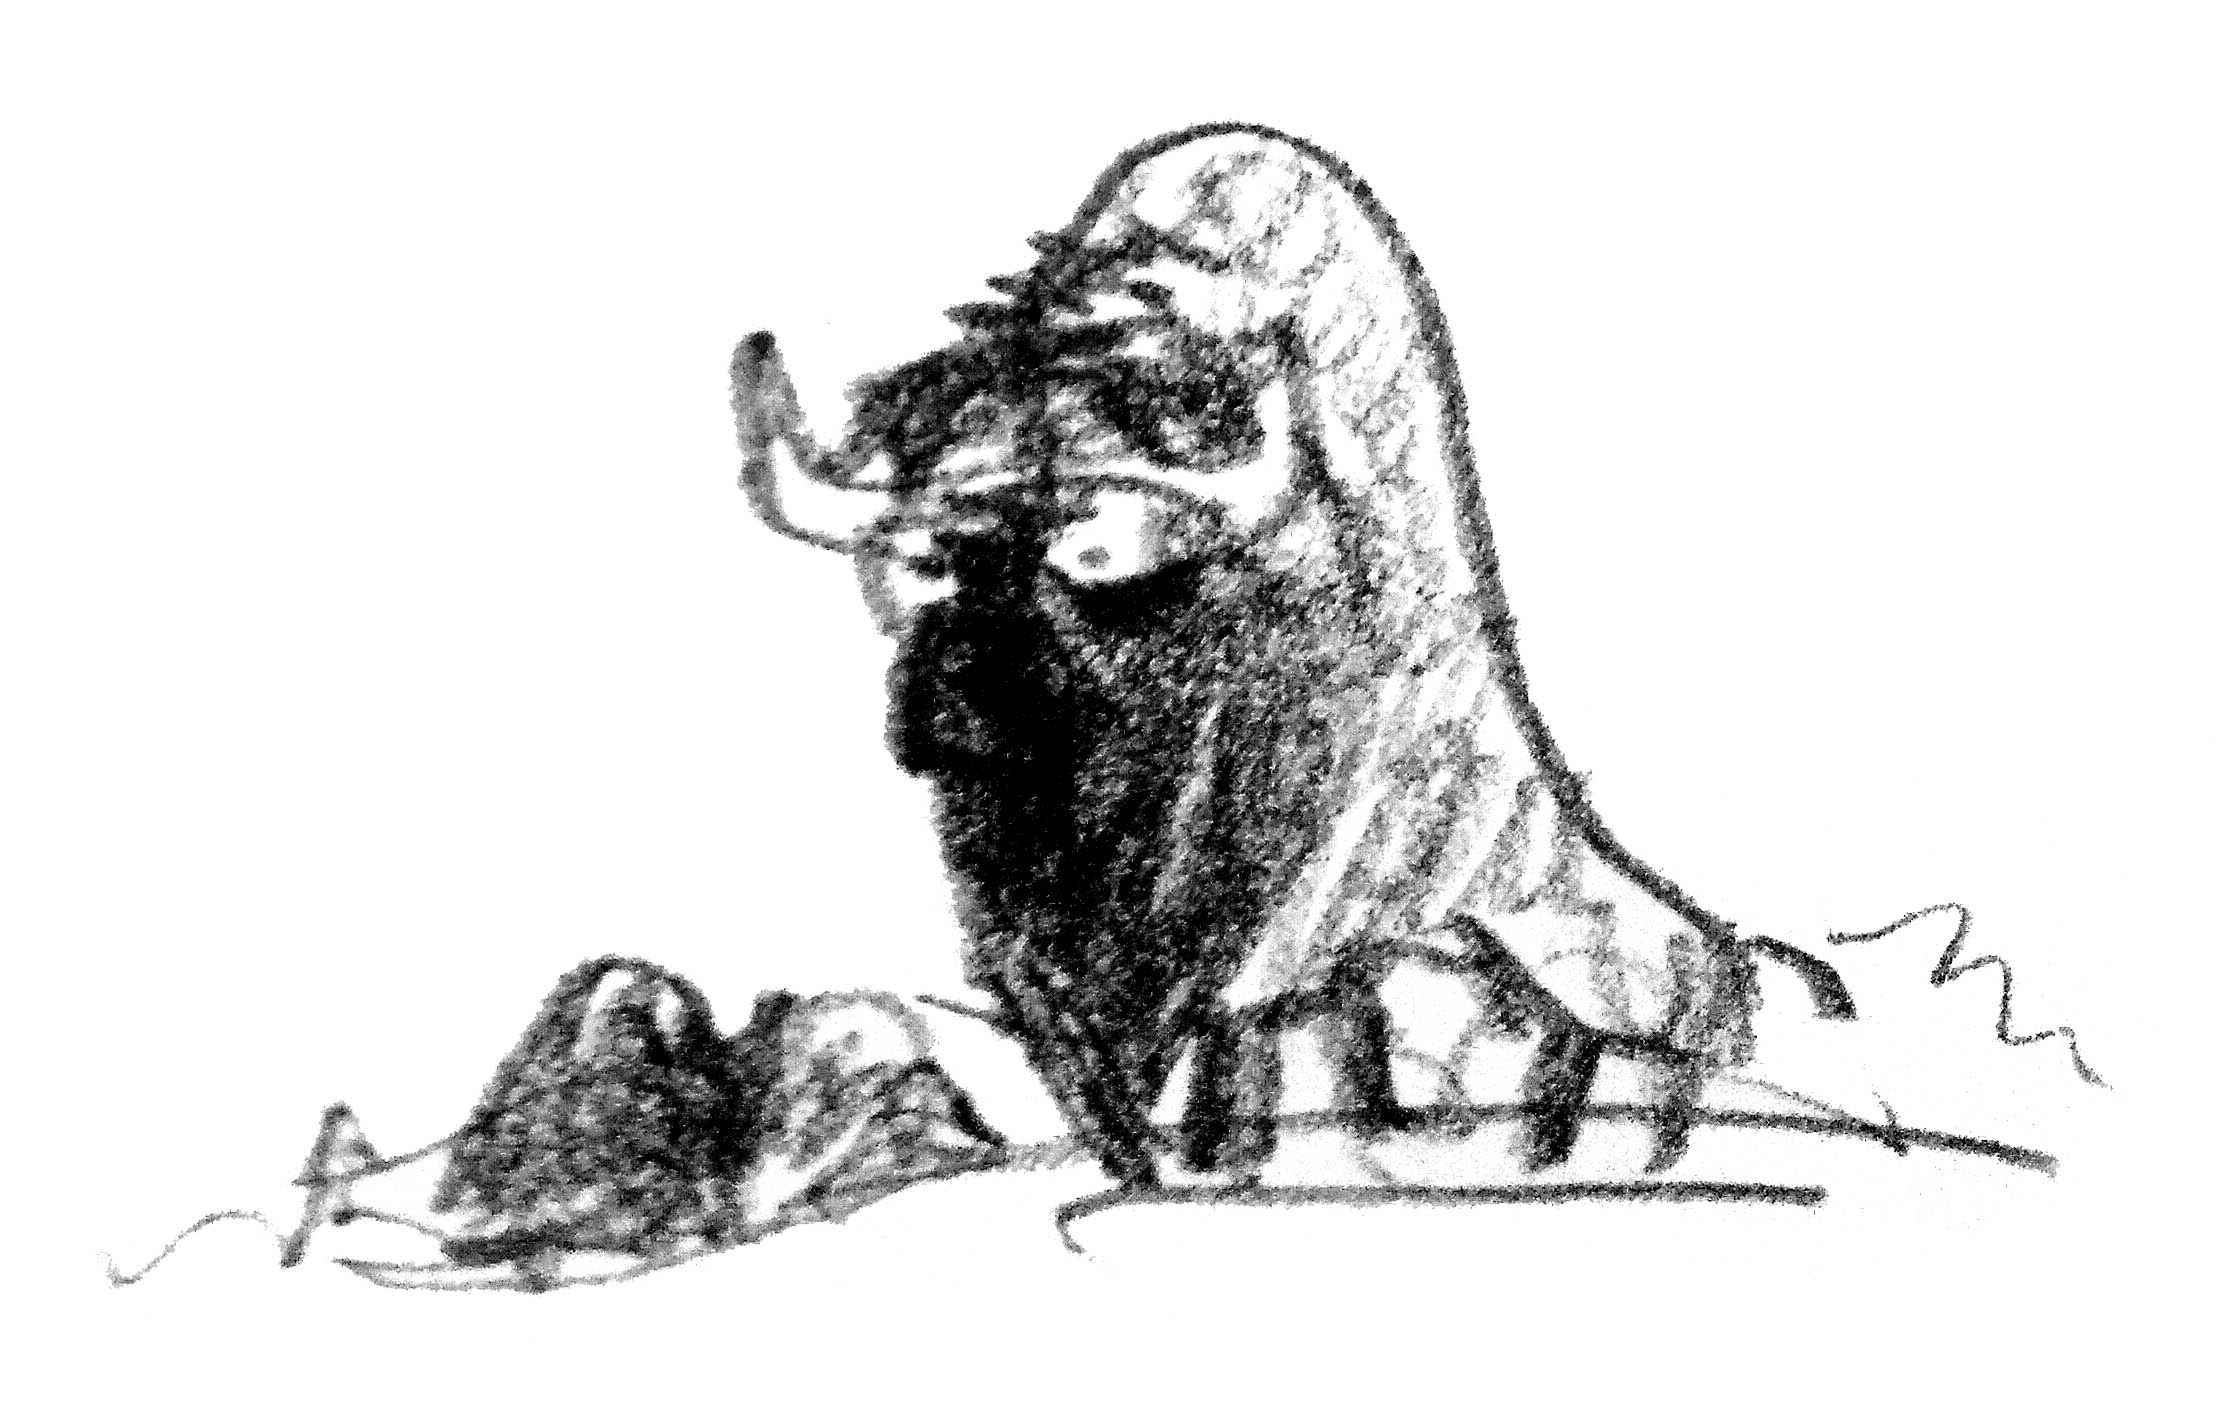
\includegraphics[width=52mm]{bison/bison-logo}\\\footnotesize\hphantom{.}\hfill---Lucas Hartmann}

\vspace*{-\baselineskip}
\newthought{Synopsis}\hspace{1.5em}
Our main contribution is a block cipher instance of the \WSN/ construction which allows us to give a strong bound on the best differential over several rounds of the cipher.
This chapter is based on the paper
\begin{quote}
    \fullfullcite{EC:CLLNW19}.
\end{quote}
All authors contributed equally.

After recalling the \WSN/ construction, we identify inherent restrictions and define a family of \WSN/ instances fulfilling these restrictions.
Subsequently, we discuss the differential cryptanalysis of these \enquote{\bison/-like} instances.
Following this analysis, we give two concrete species of \bison/-like block ciphers: \bison/ (with odd block length) and \wisent/ (with even block length).
For both we report on further cryptanalysis and give some remarks on implementation figures.

\section{Introduction}

In the context of \crefName{prob:cipher_constructions} an interesting result is the construction by \textcite{AC:Tessaro15}.
His construction is based on the Swap-or-Not construction by \textcite{C:HoaMorRog12}, which was designed for the setting where the component functions are secret.
Instead of being based on random permutations, this construction requires only a set of random (Boolean) functions.
Tessaro's construction, coined \WSNf/, requires only two public random (Boolean) functions $f_i$ with $n$-bit input, and can be proven to achieve full security, see \cref{sec:bison:wsn} for more details.

However, and this is the main motivation for our work, \emph{no instance of this construction is known}.
This situation is in sharp contrast to the case of the iterated Even-Mansour construction, where many secure instances are known for a long time already, as discussed in the previous chapter.

Without such a concrete instance, the framework of~\cite{AC:Tessaro15} remains of no avail.
As soon as one wants to use the framework in any way, one fundamentally has to instantiate the Boolean functions modeled as ideal functionalities by efficiently computable functions.
Clearly, the above mentioned bound in the ideal model does not say anything about any concrete instance.
Tessaro phrases this situation as follows:
\begin{quote}
    Heuristically, however, one hopes for even more: Namely, that under a careful implementation of the underlying component, the construction retains the promised security level.
    \hfill{}\cite{AC:Tessaro15}
\end{quote}

There has actually been one instance~\cite{C:HoaMorRog12} of the previous construction, but this has been broken almost instantaneously and completely, as parts of the encryption function were actually linear, see~\cite{C:Vaudenay12rump}.
This failure to securely instantiate the construction points to an important hurdle.
Namely, proving the generic bounds and analysing the security of an instance are technically very different tasks.
The security of any block cipher is with the current state of knowledge always the security against known attacks.
In particular, when designing any concrete block cipher, one has to argue why linear and differential attacks do not threaten the construction.

\newthoughtpar{Our Contribution}
Consequently, we investigate the important, but so far overlooked, aspect of instantiating the \WSN/ construction with a practical secure instance.
Practical secure meaning, just like in the case of \AES/, that the block cipher resists all known attacks.
We denote this instance as \bison/.\footnote{%
    For \enquote{Bent whItened Swap Or Not}
}
Our insights presented here are twofold.

First, we derive some inherent restrictions on the choice of the round function~$f_i$.
In a nutshell, we show that $f_i$ has to be rather strong, in the sense that its output bit has to basically depend on all input bits.
Moreover, we show that using less than $n$ rounds will always result in an insecure construction.
Those, from a cryptanalytic perspective rather obvious, results  are presented in \cref{bison:sec:restrictions}.
Again, but from a different angle, this situation is in sharp contrast to key-alternating ciphers.
In the case of key-alternating ciphers, even with a rather small number of rounds (\eg/~ten in the case of \AES/-128) and rather weak round functions (in case of the \AES/ round function any output bit depends on $32$~input bits only and the whole round function decomposes into four parallel functions on $32$~bits each) we get ciphers that provide, to the best of our knowledge today and after a significant amount of cryptanalysis, full security.

Second, despite those restrictions of the \WSN/ construction, that have significant impact on the performance of any instance, there are very positive aspects of the \WSN/ construction as well.
In \cref{bison:sec:dc}, we first define a family of \WSN/ instances which fulfill our initial restrictions.

As we will show in detail, this allows to argue very convincingly that our instance is secure against differential attacks.
Indeed, under standard assumptions, we can show that the probability of any (non-trivial) \emph{differential} is upper bounded by $2^{-n+1}$ where \(n\) is the block size, a value that is close to the ideal case.
% there exist no high probable {\emph{differential}} for any number of rounds $r\ge n$.
This significantly improves upon what is the state of the art for key-alternating ciphers.
As finding a solution to \crefName{prob:differentials} is notoriously hard, normally one therefore has to restrict to bounding the probability of \emph{differential characteristics} only.
Whereas our results for differential cryptanalysis gives a much simpler solution to \cref{prob:differentials}.
Additionally they can be of independent interest in the analysis of maximally unbalanced Feistel networks or nonlinear feedback shift registers.

We specify our concrete instance as a family of block ciphers for varying input length in \cref{sec:bison:instance}.
In our instance, we attach importance to simplicity and mathematical clarity.
It is making use of bent functions for instantiating $f$ and \LFSRp/ for generating the round keys.
Another advantage of \bison/ is that it defines a whole family of block ciphers, one for any odd block size.
In particular it allows the straightforward definition of small scale variants to be used for experiments.

Finally we discuss various other attacks and argue why they do not pose a threat for \bison/ in \cref{sec:bison:analysis}.
Particularly the discussion on algebraic attacks might be of independent interest.
For this we analyse the growth of the algebraic degree over the rounds.
In contrast to what we intuitively expect -- an exponential growth (until a certain threshold) as in the case for \SPNp/~\cite{FSE:BouCanDeC11} -- the degree of the \WSN/ construction grows linearly in the degree of the round function $f_i$.
This result can also be applied in the analysis of maximally unbalanced Feistel networks or nonlinear feedback shift registers.

Additionally to the results in~\cite{EC:CLLNW19}, we given an even block length instance, \wisent/, of the \WSN/ construction, see \cref{sec:wisent:instance}.
We conclude this section by adjusting our security and implementation analysis to this new instance.


\newthoughtpar{Related Work}
The first cipher, a Feistel structure, that allowed similarly strong arguments against differential attacks was presented by Nyberg and Knudsen~\cite{JC:NybKnu95}, see also~\cite{FSE:Nyberg12} for a nice survey on the topic.
This cipher was named CRADIC, as Cipher Resistant Against DIfferential Cryptanalysis but is often simply referenced as the KN cipher.
However, the cipher has been broken quickly afterwards, with the invention of interpolation attacks~\cite{FSE:JakKnu97}.
Another, technically very different approach to get strong results on resistance against attacks we would like to mention is the decorrelation theory~\cite{STACS:Vaudenay98}.
Interestingly, both previous approaches rely rather on one strong component, \ie/ round function, to ensure security, while the \WSN/ approach, and in particular \bison/, gains its resistance against differential attacks step by step.

Regarding the analysis of differentials, extensive efforts have been expended to evaluate the \MEDP//\MELP/ of \SPN/ ciphers, and in particular of the \AES/.
Some remarkable results were published by~\cite{FSE:PSLL03} and then subsequently improved by~\cite{IETIS:KelSui07} with a sophisticated pruning algorithm.
Interestingly, further work by~\cite{SCN:DaeRij06} and later by~\cite{EC:CanRou15} revealed that such bounds are not invariant under affine transformations.
All these works stress out how difficult it is to evaluate the \MEDP//\MELP/ of \SPNp/, even for a small number of rounds.
On the contrary, and as we are going to elaborate in the remaining of this paper, computing the \MEDP/ of \bison/ is rather straightforward and independent of the exact details of the components.
This can be compared to the wide trail strategy that, making use of the branch number and the superbox argument, allows bounding the probability of any differential characteristic for a large class of \SPNp/.
Our arguments allow to bound the differential probability for a large class of \WSN/ instances.

Before discussing our analysis in detail, we shortly recapitulate the \WSN/ construction.

\section{The Whitened Swap-or-Not construction}\label{sec:bison:wsn}

The \WSN/ construction is defined as follows.
Given two round keys $k_i$, $w_i$, the $i$-th round $R_{k_i,w_i}$ computes
\begin{align*}
    R_{k_i,w_i} : \F_2^n &\to \F_2^n \\
    R_{k_i,w_i}(x) &\coloneqq x + f_{b(i)}(w_i + \max\set{x, x + k_i}) \cdot k_i
\end{align*}
where $f_{0,1} : \F_2^n \to \F_2$ are modeled as two ideal random functions, the $\max$ function returns the lexicographic biggest value in the input set.
The index $b(i)$ equals zero for the first half of the rounds and one for the second half (see \cref{bison:fig:WSN} for a graphical overview of the encryption process).

In the remainder of the paper, we denote by $E_{k,w}^r(x)$ the application of $r$ rounds of the construction to the input $x$ with round keys $k_i$ and $w_i$ derived from the master key $(k,w)$.
Every round is involutory, thus for decryption one only has to reverse the order of the round keys.

\marginpar{%
    \centering
    \begin{tikzpicture}
        \node (input1) {$x$};

        \node (f1) [right=0.5em of input1, yshift=-1.5em] {$f_0$};
        \node (f1left) [left=0.5em of input1, yshift=-1.5em, color=white] {$f_0$};
        \draw [latex-latex] (f1left) edge[out=-45, in=-135, looseness=1.4] (f1);

        \draw (input1)
            -- +(0, -2.5em) node (f1split) {}
            -- +(1em, -3.5em) node [xshift=5pt] (f1_1) {\scriptsize $1$}
            -- +(1em, -5em) node [XOR, scale=0.8] (f1xor) {}
            -- (f1xor.center)
            -- +(0em, -1.5em)
            -- +(-1em, -2.5em) node (f1merge) {}
            -- +(-1em, -4em) node (input2) {};
        \draw [dashed] (f1split.center)
            -- +(-1em, -1em) node [xshift=-5pt] (f1_0) {\scriptsize $0$}
            -- +(-1em, -4em)
            -- (f1merge.center);

        \node (k1) [right=1.5em of f1xor] {$k_1$};
        \draw [-latex] (k1) -- ($(f1xor)+(8pt,0pt)$);


        \node (f2) [below=5.5em of f1] {$f_0$};
        \node (f2left) [below=5.5em of f1left, color=white] {$f_0$};
        \draw [latex-latex] (f2left) edge[out=-45, in=-135, looseness=1.4] (f2);

        \draw (input2.center)
            -- +(0, -0.5em) node (f2split) {};
        \draw [dashed] (f2split.center)
            -- +(1em, -1em) node [xshift=5pt] (f2_1) {\scriptsize $1$}
            -- +(1em, -2.5em) node [XOR, scale=0.8] (f2xor) {}
            -- (f2xor.center)
            -- +(0em, -1.5em)
            -- +(-1em, -2.5em) node (f2merge) {};
        \draw (f2merge.center)
            -- +(0em, -1em) node (output2) {};
        \draw (f2split.center)
            -- +(-1em, -1em) node [xshift=-5pt] (f2_0) {\scriptsize $0$}
            -- +(-1em, -4em)
            -- (f2merge.center);

        \node (k2) [right=1.5em of f2xor] {$k_2$};
        \draw [-latex] (k2) -- ($(f2xor)+(8pt,0pt)$);


        \node (dots) [below=-10pt of output2] {$\vdots$};

        \node (input3) [below=4pt of dots] {};

        \node (f3) [below=7em of f2] {$f_1$};
        \node (f3left) [below=7em of f2left, color=white] {$f_1$};
        \draw [latex-latex] (f3left) edge[out=-45, in=-135, looseness=1.4] (f3);

        \draw ($(input3.north)+(0,0.5em)$)
            -- +(0, -1em) node (f3split) {}
            -- +(1em, -2em) node [xshift=5pt] (f3_1) {\scriptsize $1$}
            -- +(1em, -3.5em) node [XOR, scale=0.8] (f3xor) {}
            -- (f3xor.center)
            -- +(0em, -1.5em)
            -- +(-1em, -2.5em) node (f3merge) {};
        \draw [-latex] (f3merge.center)
            -- +(0em, -1.5em) node (output4) {};
        \draw [dashed] (f3split.center)
            -- +(-1em, -1em) node [xshift=-5pt] (f3_0) {\scriptsize $0$}
            -- +(-1em, -4em)
            -- (f3merge.center);

        \node (k3) [right=1.5em of f3xor] {$k_r$};
        \draw [-latex] (k3) -- ($(f3xor)+(8pt,0pt)$);

        \node [below=-5pt of output4] {$E_{k,w}^r(x)$};
    \end{tikzpicture}
    \captionof{figure}{%
        Schematic view of the \WSNs/ construction.
    }\label{bison:fig:WSN}
}

Note that the usage of the maximum function is not decisive; it can be replaced by any function $\Phi_k$ that returns a unique representative of the set $\set{x, x+k}$, see~\citeonly{AC:Tessaro15}.
In other words it can be replaced by any function such that $\Phi_k(x) = \Phi_k(y)$ if and only if  $y \in \{x,x+k\}$.

The main result given by Tessaro on the security of the \WSN/ is the following (we only cite the informal statement, as our focus is not on the provable security aspect, but on practical instances).
\begin{proposition}[Security of the \WSN/ construction (Informal)~\citeonly{AC:Tessaro15}]
    The \WSN/ construction with $\Theta(n)$ rounds\footnote{%
        \citeauthor{AC:Tessaro15} claims security for $\mathcal{O}(n)$ rounds and notes that $\Omega(n)$ rounds are necessary to achieve information theoretically indistinguishability, as for a single query the internal Boolean function $f$ can only supply at most one bit of randomness.
    } is $(2^{n-\mathcal{O}(\log n)}, 2^{n-\mathcal{O}(1)} )$-secure.
\end{proposition}
Thus, any adversary trying to distinguish the \WSN/ construction from a random permutation and making at most $2^{n-\mathcal{O}(\log n)}$ queries to the block cipher and $2^{n-\mathcal{O}(1)}$ queries to the underlying function has negligible advantage.
Here, the round keys are modeled as independent and uniformly distributed random variables.

While \citeauthor{AC:Tessaro15}'s result gives us a strong security guarantee, the generic construction is not a practical instance.
Any practical block cipher has to provide security arguments against known attacks and, even more important, it has to give concrete details about the building blocks involved -- in this case the key schedule, the Boolean functions $f_0$ and $f_1$, and the actual number of rounds used.
To fill this gap between theory and practice here, we now analyse which generic properties any \WSN/ instance has to fulfill, and then give concrete instances of it.

\section{Inherent Restrictions}\label{bison:sec:restrictions}
In this section we point out two inherent restrictions on any practical secure instance.
Those restrictions result in general conditions on both the minimal number of rounds to be used and general properties of the round functions~$f_{b(i)}$.
In particular, those insights are taken into account for \bison/ and \wisent/.
While these restrictions are rather obvious from a cryptanalytic point of view, they have a severe impact on the performance of any concrete instance.
We discuss performance in more detail in \cref{sec:bison:implementation}.

\subsection{Number of Rounds}
As in every round of the cipher, we simply add (or not) the current round key~$k_i$, the ciphertext can always be expressed as the addition of the plaintext and a (message dependent) linear combination of all round keys $k_i$.
The simple but important observation to be made here is that, as long as the round keys do not span the full space, the block cipher is easily attackable.

Phrased in terms of linear cryptanalysis we start with the following lemma.
\begin{lemma}\label{lem:wsn:prob_one_mask}
    For any number of rounds $r<n$ there exists an element $u \in \F_2^n\setminus\{0\}$ such that
    \begin{equation*}
        \FC{E_{k,w}^r}(u,u)=2^n,
    \end{equation*}
    that is the equation
    \begin{equation*}
        \iprod{u}{x} = \iprod{u}{E_{k,w}^r(x)}
    \end{equation*}
    holds for all $x \in \F_2^n$.
\end{lemma}
\begin{proof}
    Let $k_1, \dots, k_{r}$ be the round keys derived from $k$ and denote by
    \begin{equation*}
        U = \Span{k_1, \dots, k_{r}}^{\perp}
    \end{equation*}
    the dual space of the space spanned by the round keys.
    As $r<n$ by assumption, the dimension of $\Span{k_1, \dots, k_{r}}$ is smaller than $n$ and thus $U \neq \set{0}$.
    Therefore, $U$ contains a non-zero element
    \begin{equation*}
        u \in \Span{k_1, \dots, k_{r}}^{\perp}
    \end{equation*}
    and it holds that
    \begin{equation*}
        \iprod{u}{E_{k,w}^r(x)}
        = \iprod{u}{(x + \sum_{i=1}^{r} \lambda_i k_i)}
        = \iprod{u}{x} + \iprod{u}{\sum_{i=1}^{r} \lambda_i k_i}
        = \iprod{u}{x}
    \end{equation*}
    concluding the proof.
\end{proof}

Even more importantly, this observation leads directly to a known plaintext attack with very low data-complexity.
Given a set of $t$ plaintext/ciphertext $(p_i,c_i)$ pairs, an attacker simply computes
\begin{equation*}
    V = \Span{p_i+c_i \given 1 \leqslant i \leqslant t} \subseteq \Span{k_j \given 1 \leqslant j \leqslant r}.
\end{equation*}
Given $t > r$  slightly more pairs than rounds, and assuming that $p_i+c_i$ is uniformly distributed in $\Span{k_j}$ (otherwise the attack only gets even stronger)\footnote{%
    For example if, with high probability, the $p_i + c_i$ do not depend on one or more $k_j$'s, the described attack can be extended to one or more rounds with high probability.
}
implies that
\begin{equation*}
    V= \Span{k_j}
\end{equation*}
with high probability and $V$ can be efficiently computed.
Furthermore, as above $\dim(\Span{k_j})$ is at most $r$, we have $V^{\perp} \ne \{0\}$.
Given any $u \ne 0$ in $V^\perp$ allows to compute one bit of information on the plaintext given only the ciphertext and particularly distinguish the cipher from a random permutation in a chosen-plaintext setting efficiently.

A similar argument shows the following:
\begin{lemma}\label{lem:wsn:zero_cor}
    For any number of rounds $r$ smaller than $2n-3$ there exist nonzero $\alpha$ and $\beta$, such that
    \begin{equation*}
        \widehat{E_{k,w}^r}(\alpha, \beta) = 0\;.
    \end{equation*}
\end{lemma}
\begin{proof}
    We restrict to the case $r \geqslant n$ as otherwise the statement follows directly from the lemma above.
    Indeed, from Parseval's equality, the fact that $\widehat{E_{k,w}^r}(\alpha, \alpha)=2^n$ implies that $\widehat{E_{k,w}^r}(\alpha, \beta)=0$ for all $\beta \neq \alpha$.
    Let $k_1, \ldots, k_{r}$ be the round keys derived from $k$ and choose non-zero elements $\alpha \ne \beta$ such that
    \begin{equation*}
        \alpha \in \Span{k_1, \dots, k_{n-2}}^{\perp} \qquad
        \text{and} \qquad
        \beta \in \Span{k_{n-1}, \dots, k_{r}}^{\perp}.
    \end{equation*}
    Note that, as $r \le 2n-3$ by assumption such elements always exist.
    Next, we split the encryption function in two parts, the first $n-2$ rounds $E_1$ and the remaining $r-(n-2)<n$ rounds $E_2$, i.e.
    \begin{equation*}
        E_{k,w}^r = E_2 \circ E_1.
    \end{equation*}
    We can compute the Fourier coefficient of $E_{k,w}^r$ as
    \begin{equation*}
        \FC{E_{k,w}^r}(\alpha,\beta)=\sum_{\gamma \in \F_2^n} \frac{\FC{E_1}(\alpha,\gamma)}{2^n} \cdot \frac{\FC{E_2}(\gamma,\beta)}{2^n}.
    \end{equation*}
    Now, the above lemma and the choices of $\alpha$ and $\beta$ imply that $\FC{E_1}(\alpha,\gamma) = 0$ for $\gamma \ne \alpha$ and  $\FC{E_2}(\gamma,\beta) = 0$ for $\gamma \ne \beta$.
    Recalling that $\alpha \ne \beta$ by construction concludes the proof.
\end{proof}

However, as the masks $\alpha$ and $\beta$ depend on the key, and unlike above there does not seem to be an efficient way to compute those, we do not see a direct way to use this observation for an attack.

Summarising the observations above, we get the following conclusion:
\begin{rationale}\label{rat:wsn:one}
    Any practical instance must iterate at least $n$ rounds.
    Furthermore, it is beneficial if any set of $n$ consecutive round keys are linearly independent.\footnote{%
        If (some) round keys are linearly dependent, \cref{lem:wsn:prob_one_mask,lem:wsn:zero_cor} can easily be extended to more rounds.
    }
\end{rationale}

After having derived basic bounds on the number of rounds for any secure instance, we move on to criteria on the round function itself.

\subsection{Round Function}
Here, we investigate a very basic criterion on the round function, namely dependency on all input bits, when the round function of $E^r_{k,w}$ is defined by
\begin{equation*}
    R_{k_i,w_i}(x) = x + f_{b(i)}(w_i + \max\set{x, x + k_i}) \cdot k_i\;.
\end{equation*}
Given the Boolean functions $f_{b(i)}:\F_2^n \to \F_2$, the question we would like to discuss is if it is necessary that the output bit of $f_{b(i)}$ has to depend on all input bits.
The function $f_{b(i)}$ depends on an input bit $j$ if there are two inputs $x,x'$ differing only in the $j$th bit such that $f_{b(i)}(x)\ne f_{b(i)}(x')$.
Otherwise the function is independent of the $j$th bit and we get
\begin{equation*}
    f_{b(i)}(x) = f_{b(i)}(x+e_j)
\end{equation*}
for all $x$.

We denote by $N(x) \coloneqq \set{i \given x[i] = 1}$ the index set of 1-bits in $x$, and by $\nu(x) \coloneqq \max N(x)$ the index of the highest 1-bit in $x$, in other words $\nu(x) = \floor{\log_2(x)}$, when interpreting $x \in \F_2^n$ as an integer.
For the main observation on this criterion, we first need the following lemma.
\begin{lemma}
\label{bison:lem:max_diff}
    Let $x, \delta \in \F_2^n$ and $k$ uniformly randomly drawn from $\F_2^n$.
    Then
    \begin{equation*}
        \Pr\bracket{\max\{x+\delta,x+\delta+k\}=\max\{x,x+k\}+\delta} \geqslant 1-2^{\nu(\delta)-n}.
    \end{equation*}
\end{lemma}
\begin{proof}
    The equality depends on the highest bit of $\delta$ where $x$ and $x + k$ differ, which is basically $\nu(k)$.
    We have
    \begin{equation*}
        \Pr\bracket{\max\{x+\delta,x+\delta+k\}=\max\{x,x+k\}+\delta} = \Pr\bracket{\delta[\nu(k)] = 0},
    \end{equation*}
    which can also be written as
    \begin{equation*}
        \Pr\bracket{\delta[\nu(k)] = 0}
        %= \Pr\bracket{\nu(k) \notin N(\delta)}
        = 1 - \Pr\bracket{\nu(k) \in N(\delta)}
        = 1 - \sum_{i \in N(\delta)} \Pr\bracket{\nu(k) = i}.
    \end{equation*}
    Further we have $\Pr\bracket{\nu(k) = i} = 2^{i-n-1}$ and thus
    \begin{equation*}
        1 - \sum_{i \in N(\delta)} \Pr\bracket{\nu(k) = i} = 1 - \sum_{i \in N(\delta)} 2^{i - n - 1} \geqslant 1 - 2^{\nu(\delta) - n},
    \end{equation*}
    which concludes the proof.
\end{proof}

As we will see next, the functions $f_{b(i)}$ have to depend virtually on all \emph{linear combinations of bits}.
In other words, it is required that the functions $f_{b(i)}$ have no (non-trivial) derivative equal to the all-zero function.

\begin{lemma}
    If there exists a $\delta\in\F_2^n$ such that
    \begin{equation*}
        f_{b(i)}(x) = f_{b(i)}(x+\delta)
    \end{equation*}
    for all $x$ and $i\in \set{0,1}$ then
    \begin{equation*}
        \Pr\bracket{E_{k,w}^r(x)+E_{k,w}^r(x+\delta)=\delta} \geqslant \parens{1-2^{\nu(\delta)-n}}^{r}
    \end{equation*}
    where the probability is over the input $x$ and the keys $k$ and $w$.
\end{lemma}
\begin{proof}
    From \cref{bison:lem:max_diff} we have that
    \begin{equation*}
        \Pr\bracket{\max\{x+\delta,x+\delta+k\}=\max\{x,x+k\}+\delta} \geqslant 1-2^{\nu(\delta)-n}.
    \end{equation*}
    Now, we get for one round
    \begin{equation*}
        R_{k_i,w_i}(x) = x + f_{b(i)}(w_i + \max\set{x, x + k_i}) \cdot k_i
    \end{equation*}
    by the assumption that $f_{b(i)}(x)=f_{b(i)}(x+\delta)$ for all $x$
    \begin{equation*}
        R_{k_i,w_i}(x+\delta)= R_{k_i,w_i}(x)+\delta
    \end{equation*}
    with the same probability.
    Thus, for $r$ rounds and uniformly chosen keys, we get
    \begin{equation*}
        \Pr\bracket{E_{k,w}^r(x)+E_{k,w}^r(x+\delta)=\delta} \geqslant \parens{1-2^{\nu(\delta)-n}}^{r}
    \end{equation*}
    by induction.
\end{proof}

As an example, considering the case $n=128$, $r$ rounds, and both $f_0$ and $f_1$ that do not depend on the most significant byte.
Thus, we can choose $\delta = e_{121}$ as a unit vector with $\nu(\delta)=121$ and get a differential probability of
\begin{equation*}
    \Pr\bracket{E_{k,w}^r(x)+E_{k,w}^r(x+\delta)=\delta} \geqslant \parens{1-2^{121-128}}^{r} \approx \parens{0.36}^{r/n}
\end{equation*}
which would completely compromise the scheme for a reasonable number of rounds.
In general this shows that as long as both $f_{b(i)}$ do not depend on almost all bits, the scheme is immediately broken by differential cryptanalysis.
Now, one might hope that one could craft functions $f_0$ and $f_1$ where, \eg/ $f_0$ depends only on the first $\frac{n}{2}$ bits and $f_1$ on the last $\frac{n}{2}$ bits to overcome this restriction.
However, while such a construction might be secure against basic differential cryptanalysis, it would still be completely broken by boomerang attacks~\cite{FSE:Wagner99}.
The main idea of boomerang attacks is to split the whole block cipher in two parts such that one has a high probable differential for the first part and a second high probable differential for the second part, which is exactly the situation one would end up here.

Thus, both functions independently have to virtually depend on all input bits, and we deduce the following.
\begin{rationale}\label{rat:wsn:two}
    For a practical instance, the functions $f_{b(i)}$ has to depend on all bits.
    Even more, for any $\delta \in \F_2^n$ the probability of
    \begin{equation*}
        f_{b(i)}(x)=f_{b(i)}(x+\delta)
    \end{equation*}
    should be close to $\frac{1}{2}$.
\end{rationale}

It is worth noticing that the analysis leading to this rationale applies to the original round function.
However, as pointed out in~\cite[Section~3.1]{AC:Tessaro15}, in the definition of the round function, we can replace the function
\begin{equation*}
    x \mapsto \max\set{x, x + k}
\end{equation*}
by any function $\Phi_k$ such that $\Phi_k(x)=\Phi_k(x+k)$ for all~$x$.
While the following sections will focus on the case when $\Phi_k$ is linear, we proved that \cref{rat:wsn:two} is also valid in this other setting.

Again, this should be compared to key-alternating ciphers, where usually not all output bits of a single round function depend on all input bits.
For example for \AES/ any output bit after one round depends only on $32$ input bits and for \present/ any output bit only depends on $4$ input bits.
However, while for key-alternating ciphers this does not seem to be problematic, and indeed allows rather weak round functions to result in a secure scheme, for the \WSN/ construction the situation is very different.

Before specifying our exact instance, we want to discuss differential cryptanalysis of a broader family of instances.

\section{Differential Cryptanalysis of \bison/-like instances}\label{bison:sec:dc}
We coin an instance of the \WSN/ construction \enquote{\bison/-like}, if it iterates at least $n$ rounds with linearly independent round keys $k_1, \ldots, k_n$ and applies Boolean functions $f_{b(i)}$ that depend on all bits, \ie/ fulfill \cref{rat:wsn:two}.
As explained in~\cite[Section~3.1]{AC:Tessaro15}, in order to enable decryption it is required that the Boolean functions $f_{b(i)}$ return the same result for both $x$ and $x+k$.
In the original proposition by Tessaro, this is achieved by using the $\max$ function in the definition of the round function.
Using this technique reduces the number of possible inputs for the $f_{b(i)}$ to $2^{n-1}$.
To simplify the analysis and to ease notation, we replace the $\max$ function with a \emph{linear function} $\Phi_k : \F_2^n \to \F_2^{n-1}$ with $\Ker \Phi_k = \set{0,k}$.
From now on, we assume that any \bison/-like instance uses such a $\Phi_k$ instead of the $\max$ function.
The corresponding round function has then the following form
\begin{equation}
  R_{k_i, w_i}(x) \coloneqq x + f_{b(i)} \parens{w_i + \Phi_{k_i}\parens{x}} k_i.\label{bison:eqn:wsn_instance0}
\end{equation}

With the above conditions, any \bison/-like instance of the \WSN/ construction inherits $f$'s resistance to differential cryptanalysis, as we show in the remainder of this section.
%In particular, basing the round function on bent functions together with the fact that any $n$ consecutive round keys are linearly independent by construction nicely adds to this analysis.

For our analysis, we make two standard assumptions in symmetric cryptanalysis as mentioned above: the \emph{independence of whitening round keys} $w_i$ and the \emph{hypothesis of stochastic equivalence} with respect to these round keys.
That is, we assume round keys $w_i$ to be independently uniformly drawn and the resulting \EDP/ to equal the differential probabilities averaged over all $w$.
In the following sections, we will argue why these assumptions do fit to our design and back up the results by practical experiments (see \textsc{Experimental Results} in \cref{subsec:bison-other-attacks} and
\cite[Appendix~B]{EPRINT:CLLNW18}
%\cref{bison:app:figures}
).
For the round keys $k_i$ we do not have to make such assumptions.

We first discuss the simple case of differential behaviour for one round only and then move up to an arbitrary number of rounds and devise the number of possible output differences and their probabilities.

%In all that follows, we are interested in the EDP over all the possible $w_i$ for fixed keys $k_i$.

\subsection{From One-Round Differential Characteristics}
%Let $R_{k,w}$ denote the round function of a \bison/-like instance.
%Then, as the round function is bijective, the possible output differences for any input difference $\alpha \neq 0$ are clearly restricted to either $\alpha$, or $\alpha + k$.
Looking only at one round, we can compute the \DDT/ explicitly:

\begin{proposition}\label{prop:wsn:ddt}
    Let $R_{k_i,w_i} : \F_2^n \to \F_2^n$ be the \WSN/ round function as in \cref{bison:eqn:wsn_instance0}.
    Then its \DDT/ consists of the entries
    \begin{equation}
        \mathrm{\DDTs/}[\alpha,\beta] = \begin{cases*}
            2^{n-1} + \AC{f}(\Phi_k(\alpha)) & if $\beta = \alpha$  \\
            2^{n-1} - \AC{f}(\Phi_k(\alpha)) & if $\beta = \alpha+k$\\
                    0                        & otherwise
            \end{cases*}\;.
    \end{equation}
    \marginpar{\vspace{-4.5\baselineskip}\footnotesize$\AC{f}(\cdot)$ denotes the autocorrelation of $f$.}
    Most notably, if $f$ is bent, we have
    \begin{equation*}
        \mathrm{\DDTs/}[\alpha,\beta] = \begin{cases*}
            2^n     & if $\alpha = \beta = k$ or $\alpha = \beta = 0$ \\
            2^{n-1} & if $\beta \in \set{\alpha, \alpha + k}$ and $\alpha \not \in \Span{k}$\\
            0       & otherwise
        \end{cases*}\;.
    \end{equation*}
\end{proposition}
\begin{proof}
    We have to count the number of solutions of $R(x) + R(x + \alpha) = \beta$:
    \begin{align*}
        \mathrm{\DDTs/}[\alpha,\beta] & = \abs{\set{x \in \F_2^n \given R(x) + R(x + \alpha) = \beta}}\\
                                      & = \abs{\set{x \in \F_2^n \given \alpha + \left[f( w + \Phi_k(x)) + f( w + \Phi_k(x + \alpha))\right] \cdot k = \beta}}
    \end{align*}
    Since $f$ takes its values in $\F_2$, the only output differences $\beta$ such that $\text{\DDTs/}[\alpha,\beta]$ may differ from~$0$ are $\beta=\alpha$ and $\beta=\alpha +k$.
    When $\beta=\alpha$, we have
    %Thus we need to show that the number of $x$ for which $\Delta_\alpha(f)(x) = 0$, this is the case of $\alpha = \beta$, is either $2^n$ if $\Phi_k(\alpha) = 0$, or $2^{n-1}$ else.
    %Then the second part, there are exactly $2^{n-1}$ many $x$ for which the derivative is one and thus $\beta = \alpha + k$, follows directly.
    %f(w + \Phi_k(x)) + f(w + \Phi_k(x + \alpha)) = 0$
    \begin{align*}
        \mathrm{\DDTs/}[\alpha,\alpha] & = \abs{\set{x \in \F_2^n \given f( w + \Phi_k(x)) + f( w + \Phi_k(x + \alpha)) = 0}} \\
                                       & = \abs{\set{x \in \F_2^n \given f( w + \Phi_k(x)) + f( w + \Phi_k(x) + \Phi_k(\alpha)) = 0}} \\
                                       & = 2 \cdot \abs{\set{x^\prime \in \F_2^{n-1} \given f(x^\prime) + f(x^\prime + \Phi_k(\alpha)) = 0}} \\
                                       & = 2 \parens{2^{n-2} + \frac{1}{2} \widehat{\Delta_{\Phi_k(\alpha)}(f)}(0)} = 2^{n-1} + \AC{f}(\Phi_k(\alpha))\;.
    \end{align*}
    Similarly,
    \begin{align*}
        \mathrm{\DDTs/}[\alpha,\alpha+k] & = \abs{\set{x \in \F_2^n \given f( w + \Phi_k(x)) + f( w + \Phi_k(x + \alpha)) = 1}} \\
                                         & = 2 \parens{2^{n-2} - \frac{1}{2} \widehat{\Delta_{\Phi_k(\alpha)}(f)}(0)} = 2^{n-1} - \AC{f}(\Phi_k(\alpha))\;.
    \end{align*}
    Most notably, when $\alpha \in \set{0,k}$, $\AC{f}(\Phi_k(\alpha)) = \AC{f}(0) = 2^{n-1}$.
    Moreover, when $f$ is bent, $\AC{f}(\Phi_k(\alpha)) = 0$ for all other values of $\alpha$.
\end{proof}

\subsection{To Differentials over more Rounds}
As previously explained, it is possible to estimate the probability of a differential characteristic over several rounds, averaged over the round keys, when the cipher is a Markov cipher.
We now show that this assumption holds for any \bison/-like instance of the \WSN/ construction.

\begin{lemma}
    Let $R_{k,w} : \F_2^n \to \F_2^n$ be the \WSN/ round function as in \cref{bison:eqn:wsn_instance0}.
    For any fixed $k \in \F_2^n$ and any differential $\propDiff{\alpha}{}{\beta}$, we have that
    \begin{equation*}
        \Prob_w \left[R_{k,w}(x+\alpha) + R_{k,w}(x) =\beta\right]
    \end{equation*}
    is independent of~$x$.
    More precisely
    \begin{equation*}
        \Prob_w \left[R_{k,w}(x+\alpha) + R_{k,w}(x) =\beta\right] = \Prob_x \left[R_{k,w}(x+\alpha) + R_{k,w}(x) =\beta\right]\;.
    \end{equation*}
\end{lemma}
\begin{proof}
    We have
    \begin{align*}
           &\set{w \in \F_2^{n-1} \given \Delta_\alpha (R_{k,w})(x)=\beta} \\
        =\ &\set{w \in \F_2^{n-1} \given \parens{\Delta_{\Phi_k(\alpha)}(f)(w+\Phi_k(x))} \cdot k = \alpha + \beta}\\
        =\ &\begin{cases*}
            \emptyset & if $\beta \not \in \set{\alpha, \alpha+k}$\\
            \Phi_k(x) + \supp{\Delta_{\Phi_k(\alpha)}(f)} & if $\beta=\alpha + k$\\
            \Phi_k(x) + \parens{\F_2^{n-1} \setminus \supp{\Delta_{\Phi_k(\alpha)}(f)}} & if $\beta=\alpha$
        \end{cases*}\;.
    \end{align*}
    Clearly, the cardinality of this set does not depend on $x$. Moreover, this cardinality, divided by $2^{n-1}$, corresponds to the value of
    \begin{equation*}
        \Prob_x \bracket{R_{k,w}(x+\alpha) + R_{k,w}(x) =\beta}
    \end{equation*}
    computed in the previous proposition.
\end{proof}
By induction on the number of rounds, we then directly deduce that any \bison/-like instance of the \WSN/ construction is a Markov cipher in the sense of the following corollary.
\begin{corollary}\label{bison:coro:Markov}
    Let $E_{k,w}^i$ denote $i$~rounds of a \bison/-like instance of the \WSN/ construction with round function $R_{k_i,w_i}$.
    For any number of rounds~$r$ and any round keys $(k_1, \ldots, k_r)$, the probability of an $r$-round characteristic $\theta$ satisfies
    \begin{gather*}
            \Prob_{w}\bracket{E^i_{k,w}(x) + E^i_{k,w}(x+\theta_0)=\theta_i, \forall 1 \leqslant i \leqslant r} \\
            = \quad \prod_{i=1}^r \Prob_{x} \bracket{R_{k_i,w_i}(x) + R_{k_i,w_i}(x+\theta_{i-1}) = \theta_i}\;.
    \end{gather*}
\end{corollary}
%\ac{Maybe this proof is not needed since it is clear from the lemma?}
%\begin{proof}
%  By induction on~$r$. The case $r=1$ corresponds to the previous lemma. Let us now assume that the formula holds for any $(r-1)$-round characteristic $\delta$. The probability of the characteristic $(\delta, \delta_r)$ over $r$~rounds, $P(\delta, \delta_r)$, is given by
%  \begin{eqnarray*}
%    P(\delta, \delta_r) & = & \Prob_w \left[R_{k_r,w_r}(x_r) + R_{k_r,w_r}(x_r+\delta_{r-1})=\delta_r | x_r = E_{k,w}^{r-1}(x) \right.\\
%      & & \left.\quad \mbox{ and } E_{k,w}^{i}(x) + E_{k,w}^i(x+\delta_0) = \delta_i \forall 1 \leq i < r \right] \times P(\delta)\\
%        & = & \Prob_{w_r} \left[R_{k_r,w_r}(x_r) + R_{k_r,w_r}(x_r+\delta_{r-1})=\delta_r \right] \times P(\delta)\\
%         & = & \Prob_x \left[R_{k_r,w_r}(x) + R_{k_r,w_r}(x+\delta_{r-1})=\delta_r \right] \times P(\delta)\\
%  \end{eqnarray*}
%  where we use the fact that the probability over~$w_r$ of a one-round differential does not depend on~$x_r$.
%  \end{proof}

For many ciphers several differential characteristics can cluster in a \emph{differential} over more rounds.
This is the main reason why bounding the probability of differentials is usually very difficult if possible at all.
For \bison/-like instances the situation is much nicer; we can actually compute the \EDP/, \ie/ the probabilities of the differentials averaged over all whitening key sequences $(w_1, \ldots, w_r)$.
This comes from the fact that any differential for less than $n$ rounds contains at most one differential characteristic with non-zero probability.
To understand this behaviour, let us start by analysing the \EDP/ (averaged over the $w_i$) and by determining the number of possible output differences.

In the following, we assume that the input difference $\alpha$ is fixed, and we calculate the number of possible output differences.
We show that this quantity depends on the relation between $\alpha$ and the $k_i$.

\begin{lemma}\label{bison:lem:number_diffs}
    Let us consider $r$~rounds of  a \bison/-like instance of the \WSN/ construction with round function involving Boolean functions $f_{b(i)}$ having no (non-trivial) constant derivative.
    Assume that the first $n$ round keys $k_1, \dots, k_n$ are linearly independent, and that $k_{n+1}=k_1 + \sum_{i=2}^n \gamma_i k_i$ for $\gamma_i \in \F_2$.
    For any non-zero input difference $\alpha$, the number of possible output differences $\beta$ such that
    \begin{equation*}
        \Prob_{w,x}\bracket{E_{k,w}^r(x+\alpha) + E_{k,w}^r(x)=\beta} \neq 0
    \end{equation*}
    is
    \begin{equation*}
        \begin{cases*}
            2^r              & if $\alpha \notin \Span{k_i}$ and $r < n$, \\
            2^r - 2^{r-\ell} & if $\alpha = k_\ell + \sum_{i=1}^{\ell-1} \lambda_i^\alpha k_i$ and $r \leqslant n$, \\
            %2^n - 2^{n-\ell} &\qquad& \text{if $r > n$ and all round keys $k_{j > n}$ do not depend on $k_{i \leqslant \ell}$}, \\
            2^n-1            & if $r >n$.
        \end{cases*}
    \end{equation*}
%    where $\ell$ marks the last round key $k_\ell$ on which $\alpha$ depends.
\end{lemma}
\begin{proof}
    By combining \cref{bison:coro:Markov} and \cref{prop:wsn:ddt}, we obtain that the average probability of a characteristic $(\theta_0, \theta_1, \ldots, \theta_{r-1}, \theta_r)$ can be non-zero only if $\theta_i \in \set{\theta_{i-1}, \theta_{i-1}+k_i}$ for all $1 \leqslant i \leqslant r$.
    Therefore, the output difference $\theta_r$ must be of the form
    $\theta_r= \theta_0 + \sum_{i=1}^r \lambda_i k_i$ with $\lambda_i \in \F_2$.
    Moreover, for those characteristics, the average probability is non-zero unless there exists $1 \leqslant i < r$ such that $\abs{\AC{f_{b(i)}}(\Phi_{k_i}(\theta_i))} = 2^{n-1}$, \ie/ $\Delta_{\Phi_{k_i}(\theta_i)}(f_{b(i)})$ is constant.
    By hypothesis, this only occurs when $\theta_i \in \{0,k_i\}$, and the impossible characteristics correspond to the case when either $\theta_i=0$ or $\theta_{i+1}=0$.
    It follows that the valid characteristics are exactly the characteristics of the form
    \begin{equation*}
        \theta_i = \theta_0 + \sum_{j=1}^i \lambda_j k_j
    \end{equation*}
    where none of the $\theta_i$ vanishes.
\begin{itemize}
    \item When the input difference $\alpha \not \in \Span{k_i}$, for any given output difference $\beta = \alpha + \sum_{i=1}^r \lambda_i k_i$, the $r$-round characteristic
          \begin{equation*}
              (\alpha, \alpha + \lambda_1 k_1, \alpha+ \lambda_1 k_1+ \lambda_2 k_2, \ldots, \alpha + \sum_{i=1}^r \lambda_i k_i)
          \end{equation*}
          is valid since none of the intermediate differences vanishes.
    \item When $r \leqslant n$ and $\alpha = k_\ell + \sum_{i=1}^{\ell-1} \lambda_i^\alpha k_i$, the only possible characteristic from $\alpha$ to $\beta = \alpha + \sum_{i=1}^r \lambda_i k_i$ satisfies
          \begin{equation*}
              \theta_j = \begin{cases*}
                  \sum_{i=1}^{j} (\lambda_i + \lambda_i^\alpha)k_i + \sum_{i=j+1}^\ell \lambda_i^\alpha k_i & if $j \leqslant \ell$\\
                  \sum_{i=1}^{\ell} (\lambda_i + \lambda_i^\alpha)k_i + \sum_{i=\ell+1}^j \lambda_i k_i & if $j > \ell$\;.
              \end{cases*}
          \end{equation*}
          Since the involved round keys are linearly independent, we deduce that $\theta_j=0$ only when $j=\ell$ and $\lambda_i = \lambda_i^\alpha$ for all $1 \leqslant i \leqslant \ell$.
          It then follows that there exists a valid characteristic from $\alpha$ to $\beta$ unless $\lambda_i = \lambda_i^\alpha$ for all $1 \leqslant i \leqslant \ell$.
          The number of possible outputs $\beta$ is then
          \begin{equation*}
              (2^\ell-1)2^{r-\ell}= 2^r - 2^{r-\ell}.
          \end{equation*}
    \item If we increase the number of rounds to more than $n$, we have $\alpha = k_\ell + \sum_{i=1}^{\ell-1} \lambda_i^\alpha k_i$ for some $\ell \leqslant n$.
          If $\beta = \alpha + \sum_{i=1}^n \lambda_i k_i$ with $\sum_{i=1}^\ell \lambda_i k_i \neq \alpha$, then we can obviously extend the previous $n$-round characteristic to
          \begin{equation*}
              (\alpha, \alpha+\lambda_1 k_1, \ldots, \alpha + \sum_{i=1}^{n-1}\lambda_i k_i, \beta, \beta, \ldots, \beta).
          \end{equation*}
          If $\sum_{i=1}^\ell \lambda_i k_i = \alpha$, $\beta$ cannot be the output difference of an $n$-round characteristic.
          However, the following $(n+1)$-round characteristic starting from $\theta_0=\alpha$ is valid:
          \begin{equation*}
              \theta_j = \begin{cases*}
                k_1 + \sum_{i=2}^j \gamma_i k_i + \sum_{i=j+1}^\ell \lambda_i^\alpha k_i & if $j \leqslant \ell$\\
                k_1 + \sum_{i=2}^j \gamma_i k_i + \sum_{i=\ell+1}^j \lambda_i k_i & if $\ell < j \leqslant n$\\
                \beta & if $j=n+1$
              \end{cases*}
          \end{equation*}
          Indeed, $\theta_n = \beta+k_n$ implying that the last transition is valid.
          Moreover, it can be easily checked that none of these $\theta_j$ vanishes, unless $\beta=0$.
          This implies that all non-zero output differences $\beta$ are valid.
\end{itemize}
\vspace{-1.5\baselineskip}
\end{proof}

%In other words, the second case occurs, because for $r \leqslant n$ there is only one decomposition of $\alpha$ in the basis of the $k_i$ and thus only one branch in the tree of differences can collapse, see also the following \cref{fig:possible_output_diffs}.

The last case in the above lemma is remarkable, as it states any output difference is possible after $n+1$ rounds.
To highlight this, we restate it as the following corollary.
\begin{corollary}\label{bison:cor:no_impossible_diffs}
    For \bison/-like instances with more than $n$ rounds whose round keys $k_1, \ldots, k_{n+1}$ satisfy the hypothesis of \cref{bison:lem:number_diffs}, and for any non-zero input difference, every non-zero output difference is possible.
\end{corollary}

We now focus on a reduced version of the cipher limited to exactly $n$ rounds and look at the probabilities for every possible output difference.
Most notably, we exhibit in the following lemma an upper-bound on the \MEDP/ which is minimised when $n$ is odd and the involved Boolean functions $f_{b(i)}$ are bent.
In other words, \cref{rat:wsn:two} which was initially motivated by the analysis in \cref{bison:sec:restrictions} for the original round function based on $x \mapsto \max(x,x+k)$~\cite{AC:Tessaro15} is also valid when a linear function $\Phi_k$ is used.

%In the case of linearly independent round keys, every difference can be expressed as a linear combination of the keys.
\begin{lemma}\label{lem:bison:diff_prob}
    Let us consider $n$~rounds of a \bison/-like instance of the \WSN/ construction with round function involving Boolean functions $f_{b(i)}$.
    Let $k_1, \dots, k_n$ be any linearly independent round keys.
    Then, for any input difference $\alpha \ne 0$ and any $\beta$, we have
    \begin{align*}
        \mathrm{\EDP/}(\alpha, \beta) &= \Prob_{w,x}\bracket{E_{k,w}(x+\alpha) + E_{k,w}(x)=\beta}\\
                                    &\leqslant \parens{\frac{1}{2} + 2^{-n} \max_{1 \leqslant i \leqslant n} \absoluteindicator{f_{b(i)}}}^{n-1}\;.
    \end{align*}
    \marginpar{\vspace{-4em}\footnotesize$\absoluteindicator{f}$ denotes the absolute indicator of $f$.}
    More precisely, if all $f_{b(i)}$ are {\em bent},
    \begin{empheq}[left={\mathrm{\EDP/}(\alpha, \beta) =\empheqbiglbrace~}]{align}
            &0        &\hspace{-1cm}& \text{if $\beta = \sum_{i=\ell+1}^n \lambda_i k_i$}, \label{bison:eqn:impossible_output}\\
            &2^{-n+1} &\hspace{-1cm}& \text{if $\beta = k_\ell + \sum_{i=\ell+1}^n \lambda_i k_i$,} \label{bison:eqn:collapsed_output}\\
            &2^{-n}   &\hspace{-1cm}& \text{otherwise}, \label{bison:eqn:other_output}
    \end{empheq}
    where $\ell$ denotes as previously the latest round key that appears in the decomposition of $\alpha$ into the basis $(k_1, \ldots, k_n)$, that is $\alpha = k_\ell + \sum_{i=1}^{\ell-1} \lambda_i k_i$.
\end{lemma}
\begin{figure}[t]
    \begin{sidecaption}[Tree of possible output differences]{%
        Probabilities of output differences for three rounds and the cases of the input difference $\alpha = k_1 + k_2$, thus $\ell = 2$.
        Dotted transitions are impossible.
    }[bison:fig:possible_output_diffs]
    \centering
    \begin{forest}
        for tree={grow=east},
        [$\alpha$
            [{$\alpha$}, edge label={node[midway,below,font=\scriptsize] {$\frac{1}{2}$}}, tikz={\node[draw,gray!20,inner sep=0,fit to=tree]{};}
                [{$\alpha$}
                    [{$\alpha$}]
                    [{$\alpha + k_3$}]
                ]
                [{$\alpha + k_2$}
                    [{$\alpha + k_2$}]
                    [{$\alpha + k_2 + k_3$}]
                ]
            ]
            [{$\alpha + k_1$}, edge label={node[midway,above,font=\scriptsize] {$\frac{1}{2}$}}
                [{$\alpha + k_1$}, edge={thick}, edge label={node[midway,below,xshift=-1mm,font=\scriptsize] {$1$}}, tikz={\node[draw,gray!20,inner sep=0,fit to=tree]{};}
                    [{$\alpha + k_1$}]
                    [{$\alpha + k_1 + k_3$}]
                ]
                [{$\alpha + k_1 + k_2$}, edge={dotted}, edge label={node[midway,above,xshift=-1mm,font=\scriptsize] {$0$}}, tikz={\node[draw,gray!20,inner sep=0,fit to=tree]{};}
                    [{$\alpha + k_1 + k_2$}, edge={dotted}]
                    [{$\alpha + k_1 + k_2 + k_3$}, edge={dotted}]
                ]
            ]
        ]
        \draw[] (forest cs:l=75mm,s=22.5mm) node[right]{\cref{bison:eqn:impossible_output}};
        \draw[] (forest cs:l=75mm,s=7.5mm) node[right]{\cref{bison:eqn:collapsed_output}};
        \draw[] (forest cs:l=75mm,s=-12.5mm) node[right]{\cref{bison:eqn:other_output}};
    \end{forest}
    \end{sidecaption}
\end{figure}
The case of bent functions is visualised in \cref{bison:fig:possible_output_diffs}, where we give an example of the three possibilities for three rounds.
\begin{proof}
    As proved in \cref{bison:lem:number_diffs}, $(\alpha, \beta)$ is an impossible differential if and only if $\beta = \sum_{i=\ell + 1}^n \lambda_i k_i$.
    For all other values of $\beta = \alpha + \sum_{i=1}^n \lambda_i k_i$, we have
    \begin{equation*}
        \mathrm{\EDP/}(\alpha, \beta) = \prod_{i=1}^n \parens{\frac{1}{2} + \parens{-1}^{\lambda_i} 2^{-n} \AC{f_{b(i)}}(\Phi_{k_i}(\theta_i))}
    \end{equation*}
    where $\theta_i = \alpha + \sum_{j=1}^i \lambda_j k_j$.
    The $i$-th term in the product is upper bounded by
    \begin{equation*}
        \frac{1}{2} + 2^{-n} \max_{1 \leqslant i \leqslant n} \absoluteindicator{f_{b(i)}}
    \end{equation*}
    except if $\Phi_{k_i}(\theta_i) =0$, \ie/ $\theta_i \in \{0, k_i\}$.
    As seen in \cref{bison:lem:number_diffs}, the case $\theta_i=0$ cannot occur in a valid characteristic.
    The case $\theta_i=k_i$ occurs if and only if $i=\ell$ and $\beta = k_\ell + \sum_{j=\ell + 1}^n \lambda_j k_j$.
    In this situation, the $\ell$-th term in the product equals one.
    In the tree of differences this is visible as the collapsing of the two branches from two possible succeeding differences into only one, which then of course occurs with probability one, see upper branch of \cref{bison:fig:possible_output_diffs}.

    Most notably, all $f_{b(i)}$ are bent if and only if
    \begin{equation*}
        \max_{1 \leqslant i \leqslant n} \absoluteindicator{f_{b(i)}} = 0\;,
    \end{equation*}
    leading to the result.

    This can be seen on \cref{bison:fig:possible_output_diffs}: the $2^{n-\ell}$ possible differences coming from the collapsed branch have a transition of probability one in that round, resulting in an overall probability of $2^{-n+1}$, see \cref{bison:eqn:collapsed_output}.
    For the lower part of \cref{bison:fig:possible_output_diffs}, all the other differences are not affected by this effect and have a probability of $2^{-n}$, see \cref{bison:eqn:other_output}.
\end{proof}

Because they allow us to minimise the \MEDP/, we now concentrate on the case of bent functions for the sake of simplicity, which implies that the block size is odd.
However, for implementation reasons an even block size is typically preferred.
We discuss our \bison/-like instance with even block sizes, \wisent/, at the end of this chapter, see \cref{sec:wisent:instance}.
%However, if an even block size is more appropriate for implementation reasons, we could also define \bison/-like instances based on maximally nonlinear functions.

It would be convenient to assume in differential cryptanalysis that the \EDP/ of a differential does not increase when adding more rounds, while this does not hold in general.
However, this argument can easily be justified for \bison/-like instances using bent functions, when averaging over the whitening keys $w$.
\begin{proposition}
    Let us consider $r \geqslant n$~rounds of a \bison/-like instance of the \WSN/ construction with bent functions $f_{b(i)}$.
    Let $k_1, \dots, k_n$ be any linearly independent round keys.
    Then the probability of any non-trivial differential, averaged over all whitening key sequences $w$ is upper bounded by $2^{-n + 1}$.

    In other words, the \MEDP/ of \bison/-like instances with bent $f_{b(i)}$ for $r \geqslant n$ rounds is $2^{-n+1}$.
\end{proposition}
\begin{proof}
    By induction over $r$.
    The base case for $r=n$ rounds comes from \cref{lem:bison:diff_prob}.
    In the induction step, we first consider the case when the output difference $\beta$ after $r$~rounds differs from~$k_{r}$.
    Then the output difference $\theta_{r} = \beta$ can be reached if and only if the output difference after $(r-1)$~rounds $\theta_{r-1}$ belongs to $\{\beta, \beta + k_{r}\}$.
    Then,
    \begin{align*}
        \mathrm{\EDP/}^r(\alpha, \beta) =\ &  \Prob_{w_r} \bracket{R_{k_{r},w_r}(x_r)+ R_{k_{r},w_r}(x_r+\beta) = \beta} \mathrm{\EDP/}^{r-1}(\alpha, \beta) \\
                                         & + \Prob_{w_r} \bracket{R_{k_{r},w_r}(x_r)+ R_{k_{r},w_r}(x_r+\beta+k_r) = \beta} \mathrm{\EDP/}^{r-1}(\alpha, \beta+k_r) \\
                                      =\ & \frac{1}{2} \parens{\mathrm{\EDP/}^{r-1}(\alpha, \beta) + \mathrm{\EDP/}^{r-1}(\alpha, \beta+k_r)} \leqslant 2^{-n+1}\;.
    \end{align*}
    When the output difference $\beta$ after $r$~rounds equals~$k_r$, it results from $\theta_{r-1}=k_r$ with probability~$1$.
    In this case
    \begin{equation*}
        \mathrm{\EDP/}^r(\alpha, \beta) = \mathrm{\EDP/}^{r-1}(\alpha, \beta) \leqslant 2^{-n+1}
    \end{equation*}
    as required.
\end{proof}
This bound is close to the ideal case, in which each differential has probability $1/(2^{n}-1)$.

We now give a detailed description of our instance \bison/.

\section{Specification of \bison/}\label{sec:bison:instance}
As \bison/ should obviously be a specialisation of \bison/-like instances, this concrete instance inherits the already specified parts.
Thus \bison/, replaces the $\max$ function by $\Phi_k$, and uses a key schedule that generates round keys, where all $n$ consecutive round keys are linearly independent.
Further, as assumed at the end of the prior section, \bison/ uses two bent functions $f_{b(i)}$.
The resulting instance for $n$ bits iterates the \WSN/ round function as defined below over $3 \cdot n$~rounds.
The chosen number of rounds mainly stems from the analysis of the algebraic degree that we discuss in \cref{sec:bison:analysis}.

\subsection{Round function}
For any nonzero round key $k$, we define $\Phi_{k} : \F_2^{n} \to \F_2^{n-1}$ as
\begin{equation}\label{bison:eqn:phi}
    \Phi_{k}(x) \coloneqq (x_{i(k)} \cdot k + x)[1,\ldots,i(k)-1,i(k)+1,\ldots,n],
\end{equation}
where $i(k)$ denotes the index of the lowest bit set to 1 in $k$, and the notation $x[1,\ldots,j-1,j+1,\ldots,n]$ returns the $(n-1)$-bit vector, consisting of the bits of $x$ except the $j$th bit.

\begin{lemma}\label{bison:lem:phi_prop}
    The function $\Phi_k : \F_2^{n} \to \F_2^{n-1}$ is linear and satisfies
    \begin{equation*}
        \Ker \Phi_{k} = \set{0,k}.
    \end{equation*}
\end{lemma}
The proof can be done by simply computing both outputs for $x$ and $x+k$.

For the preimage of $y \in \F_2^{n-1}$ and $j = i(k)$ we have
\begin{equation}\label{bison:eqn:phi_preimage}
    \Phi_k^{-1}(y) \in \left\{
        \begin{aligned}
            &\parens{y[1\colon\!j-1], 0, y[j\colon\!n-1]} + k[1\colon\!n], \\
            &\parens{y[1\colon\!j-1], 0, y[j\colon\!n-1]}
        \end{aligned}
    \right\}.
\end{equation}

Due to the requirement for the $f_{b(i)}$ being bent, we are limited to functions taking an even number of bits as input.
The simplest example of a bent function is the inner product.

Eventually we end up with the following instance of the \WSN/ round.

\begin{center}
\begin{minipage}{\textwidth}
    \centering
    \textbf{\bison/'s Round Function}\\[0.5\baselineskip]
\begin{tikzpicture}
    \node[draw, rectangle, minimum width=0.95\textwidth, rounded corners=5pt, thick] {%
        \centering
        \begin{minipage}{0.90\textwidth}
            \vspace{0.5\baselineskip}
            For round keys $k_i\in \F_2^n$ and $w_i\in \F_2^{n-1}$ the round function computes
            \begin{equation}
                R_{k_i, w_i}(x) \coloneqq x + f_{b(i)} \parens{w_i + \Phi_{k_i}\parens{x}} k_i.\label{bison:eqn:wsn_instance}
            \end{equation}
            where
            \begin{itemize}
                \item $\Phi_{k_i}$ is defined as in \cref{bison:eqn:phi},
                \item $f_{b(i)}$ is defined as
                        \begin{align*}
                            f_{b(i)} : \F_2^{n-1} &\to \F_2 \\
                            f_{b(i)}(x) &\coloneqq \iprod{x[1 : (n-1)/2]}{x[(n+1)/2 : n-1]} + b(i),
                        \end{align*}
                \item and $b(i)$ is $0$ if $i \leqslant \frac{r}{2}$ and $1$ otherwise.
            \end{itemize}
            \vspace{-0.25\baselineskip}
        \end{minipage}
        };
\end{tikzpicture}
\end{minipage}
\end{center}

\begin{secclaim}[\bison/]
  We claim $n$-bit security for \bison/ in the single-key model.
  We emphasise that we do not claim any security in the related-key, chosen-key or known-key model.
\end{secclaim}

\subsection{Key schedule}
In the $i$-th round, the key schedule has to compute two round keys: $k_i \in \F_2^n$ and $w_i \in \F_2^{n-1}$.
We compute those round keys as the states of \LFSR/s after $i$ clocks, where the initial states are given by a master key $K$.
The master key consists of two parts of $n$ and $n-1$ bits, \ie/
\begin{equation*}
    K=(k,w) \in \F_2^n \times \F_2^{n-1}.
\end{equation*}
As the all-zero state is a fixed point for any \LFSR/, we \emph{exclude the zero key} for both $k$ and $w$.
In particular $k=0$ is obviously a weak key that would result in a ciphertext equal to the plaintext $p = E_{0,w}^r(p)$ for all $p$, independently of $w$ or of the number of rounds $r$.

It is well-known that choosing a feedback polynomial of an \LFSR/ to be primitive results in an \LFSR/ of maximal period.
Clocking the \LFSR/ then corresponds to multiplication of its state with the companion matrix of this polynomial.
Interpreted as elements from the finite field, this is the same as multiplying with a primitive element.

In order to avoid structural attacks, \eg/ invariant attacks~\citeonly{C:LAAZ11,AC:TodLeaSas16,ToSC:GraRecRon16}, as well as the propagation of low-weight inputs, we add round constants $c_i$ to the round key $w_i$.

These round constants are also derived from the state of an \LFSR/ with the same feedback polynomial as the $w_i$~\LFSR/, initialised to the unit vector with the least significant bit set.
To avoid synchronization with the $w_i$~\LFSR/, the $c_i$~\LFSR/ clocks backwards.
\begin{center}
    \begin{minipage}{\textwidth}
        \centering
    \textbf{\bison/'s Key Schedule}\\[0.5\baselineskip]
\begin{tikzpicture}
    \node[draw, rectangle, minimum width=0.95\textwidth, rounded corners=5pt, thick] {%
        \centering
        \begin{minipage}{0.90\textwidth}
            \vspace{0.5\baselineskip}
            For two primitive polynomials $p_w(x),\, p_k(x) \in \F_2[x]$ with degrees $\deg(p_w) = n-1$ and $\deg(p_k) = n$ and the master key $K=(k,w) \in \F_2^n\times \F_2^{n-1}$, $k,w \ne 0$
            the key schedule computes the $i$-th round keys as
            \begin{align*}
                \mathrm{KS}_i : \F_2^n \times \F_2^{n-1} &\to \F_2^n \times \F_2^{n-1} \\
                \mathrm{KS}_i(k, w) &\coloneqq ({C(p_k)}^i k, {C(p_w)}^{-i} e_1 + {C(p_w)}^i w) = (k_i, c_i + w_i)
            \end{align*}
            where $C(\cdot)$ is the companion matrix of the corresponding polynomial, and $0 \leqslant i < r$.

            In
            \citeonly[Appendix~A]{EPRINT:CLLNW18}
            %\cref{bison:app:polys}
            we give concrete polynomials for $5 \leqslant n \leqslant 129$-bit block sizes.
            \vspace{0.5\baselineskip}
        \end{minipage}
        };
\end{tikzpicture}
\end{minipage}
\end{center}

As discussed above, this key schedule has the following property, see also \cref{rat:wsn:one}.
\begin{lemma}\label{bison:lem:ks}
    For \bison/'s key schedule, the following property holds:
    Any set of $n$ consecutive round keys $k_i$ are linearly independent.
    Moreover there exist coefficients $\lambda_i$ such that
        \begin{equation*}
            k_{n+i} = k_i + \sum_{j=i+1}^{n+i-1} \lambda_j k_j.
        \end{equation*}
\end{lemma}
\begin{proof}
    To prove this, we start by showing that the above holds for the first $n$ round keys, the general case then follows from a similar argumentation.

    We need to show that there exists no non-trivial $\lambda_i \in \F_2$, $1 \leqslant i \leqslant n$, so that
    \begin{align*}
        \sum_{i=1}^{n} \lambda_i k_i = &\sum_{i=1}^{n} \lambda_i C\parens{p_{k}}^i k = 0\;, \\
        \intertext{which is equivalent to showing that there exists no non-trivial $\lambda_i \in \F_2$ such that}
        &\sum_{i=0}^{n-1} \lambda_i C\parens{p_{k}}^i k = 0\;.
    \end{align*}
    In this regard, we recall the notion of \emph{minimal polynomial of $k$ with respect to $C(p_{k})$}, defined as the monic polynomial of smallest degree $Q_L(k)(x) = \sum_{i=0}^{d} q_i x^i \in \F_2[x]$  such that $\sum_{i=0}^{d} q_i C\parens{p_{k}}^i k = 0$.
    Referring to a discussion that has been done for instance in~\cite{C:BCLR17}, we know that the minimal polynomial of $k$ is a divisor of the minimal polynomial of $C(p_{k})$.
    Since in our case our construction has been made so that this later is equal to $p_k$ which is a primitive polynomial, we deduce that the minimal polynomial of $k \ne 0$ is $p_{k}$ itself.
    Since the degree of $p_{k}$ is equal to $n$, this prove that the first $n$ keys are linearly independent.

    The equation holds, since $p_k(0) = 1$.
\end{proof}

\section{Security Analysis of \bison/}\label{sec:bison:analysis}
As we have already seen, \bison/ is resistant to differential cryptanalysis.
We next argue why \bison/ is also resistant to other known attacks.
In particular we bound the potential of any linear trail over $r$ rounds, analyse and bound the algebraic degree, discuss resistance against impossible differentials, zero correlation and invariant attacks, and analyse the related-key behaviour.

\subsection{Linear Cryptanalysis}
For linear cryptanalysis, given the fact that \bison/ is based on a bent function, \ie/ a maximally non-linear function, arguing that no linear characteristic with high correlation exist is rather easy.
Again, we start by looking at the Fourier coefficients for one round.

\newthoughtpar{From one Round}
Using the properties of $f$ being bent, we get the following.
\begin{restatable}{proposition}{probalinearcharacteristic}\label{prop:bison:lat}
    Let $R_{k,w} : \F_2^n \to \F_2^n$ be the round function as defined in \cref{bison:eqn:wsn_instance}.
    Then its \LAT/ consists of the entries
    \begin{align}\label{bison:eqn:fc_round}
        &\hphantom{=}\ \widehat{R_{k,w}}(\alpha,\beta) \nonumber \\
        &= \begin{cases*}
            2^n                    & if $\alpha = \beta$ and $\iprod{\beta}{k} = 0$ \\
            \pm2^{\frac{n+1}{2}} & if $\iprod{\alpha}{k} = 1$ and $\iprod{\beta}{k} = 1$ \\
                                        % the same as <a + b, k> = 0 and <b, k> = 1
            0                      & if $\iprod{(\alpha + \beta)}{k} = 1$ or $(\alpha \neq \beta$ and $\iprod{\beta}{k} = 0)$
        \end{cases*}.
    \end{align}
\end{restatable}
\begin{proof}
    First, we show the upper part, that is the values of the diagonal.
    Then
    \begin{align*}
        &\hphantom{=}\ \ \widehat{R_{k,w}}(\alpha, \beta)
         = \sum_{x \in \F_2^{n}} \parens{-1}^{\iprod{(\alpha + \beta)}{x} + \iprod{\beta}{k}\cdot f(w + \Phi_k(x))} \\
        &= \sum_{\tower{y \in \F_2^{n-1}}{\Phi_k^{-1}(y) \in \set{x_0, x_1}}} \parens{-1}^{\iprod{(\alpha + \beta)}{x_0} + \iprod{\beta}{k}\cdot f(w + y)} + \parens{-1}^{\iprod{(\alpha + \beta)}{x_1} + \iprod{\beta}{k}\cdot f(w + y)}
    \end{align*}
    As we look at the diagonal elements, $\alpha = \beta$, we have
    \begin{align*}
    \widehat{R_{k,w}}(\alpha, \alpha)
    = 2 \cdot \sum_{y} \parens{-1}^{\iprod{\beta}{k} \cdot f(w + y)}
    = 2 \cdot \sum_{y^\prime \in \F_2^{n-1}} \parens{-1}^{\iprod{\beta}{k} \cdot f(y^\prime)}\;.
    \end{align*}
    Two possibilities remain:
    If $\iprod{\beta}{k} = 0$, the exponent is always zero and thus $\widehat{R_{k,w}}(\alpha, \alpha) = 2^n$.
    In the other case, $\iprod{\beta}{k} = 1$ and
    \begin{equation}\label{eqn:bison:lat_proof_adjust1}
        \widehat{R_{k,w}}(\alpha, \alpha) = 2 \cdot \sum_{y^\prime \in \F_2^{n-1}} \parens{-1}^{f(y^\prime)} = \pm 2 \cdot 2^{\frac{n-1}{2}}\;,
    \end{equation}
    since Parseval's relation implies that all Fourier coefficients of an $(n-1)$-variable bent function have the same magnitude, namely $2^{\frac{n-1}{2}}$.

    Now for the second part we have $\alpha \neq \beta$.
    \begin{align}
        &\hphantom{=}\ \ \widehat{R_{k,w}}(\alpha, \beta) \nonumber\\
        &= \sum_{\tower{y \in \F_2^{n-1}}{\Phi_k^{-1}(y) \in \set{x_0, x_1}}} \parens{-1}^{\iprod{(\alpha + \beta)}{x_0} + \iprod{\beta}{k}\cdot f(w + y)} + \parens{-1}^{\iprod{(\alpha + \beta)}{x_1} + \iprod{\beta}{k}\cdot f(w + y)} \nonumber\\
        \intertext{By definition of $\Phi_k$, we saw in \cref{bison:eqn:phi_preimage} that the preimages $x_0$ and $x_1$ of $y$ are equal to $y^\prime$ and $y^\prime + k$, where $y^\prime$ is the same as $y$ with an additional bit set to zero injected at position $i(k)$.
                   Thus, using the bilinearity of the scalar product,}
        \widehat{R_{k,w}}(\alpha, \beta) &= \parens{1 + \parens{-1}^{\iprod{(\alpha + \beta)}{k}}} \sum_y \parens{-1}^{\iprod{(\alpha + \beta)}{y^\prime} + \iprod{\beta}{k} \cdot f(w + y)} \nonumber\\
        \intertext{and this is equal to zero, if $\iprod{(\alpha + \beta)}{k} = 1$ or $\iprod{\beta}{k} = 0$.
                   In the other case, $\iprod{(\alpha + \beta)}{k} = 0$ and $\iprod{\beta}{k} = 1$, we have}
        \widehat{R_{k,w}}(\alpha, \beta) &= 2 \cdot \sum_y \parens{-1}^{\iprod{(\alpha + \beta)}{y^\prime} + f(w + y)} = 2 \cdot \sum_x \parens{-1}^{\iprod{(\alpha + \beta)}{(x^\prime + w^\prime)} + f(x)} \nonumber \\
        &= 2 \cdot \parens{-1}^{\iprod{(\alpha + \beta)}{w^\prime}} \cdot \sum_x \parens{-1}^{\iprod{(\alpha + \beta)}{x^\prime} + f(x)} \nonumber \\
        & = 2 \cdot \parens{-1}^{\iprod{(\alpha + \beta)}{w^\prime}} \cdot \widehat{f}(\Phi_k(\alpha + \beta)) \label{eqn:bison:lat_proof_adjust2} \\
        \intertext{Finally, again because $f$ is bent, we get}
        \widehat{R_{k,w}}(\alpha, \beta) &= 2 \cdot \parens{-1}^{\iprod{(\alpha + \beta)}{w^\prime}} \cdot (\pm 2^{\frac{n-1}{2}}) = \pm 2^{\frac{n+1}{2}}\;. \nonumber
        &\hspace*{-15pt}
    \end{align}

    Note that the sign of the \LAT/ entries is uniformly distributed and thus, when averaging over the $w$'s, the non-diagonal entries cancel out.
\end{proof}

\newthoughtpar{To more Rounds}
When we look at more than one round, we try to approximate the linear hull by looking at the strongest linear trail.
As already discussed in \cref{lem:wsn:prob_one_mask}, for $r < n$ there are trails with probability one.
We now show that any trail's correlation for $r \geqslant n$ rounds is actually upper bounded by $2^{-\frac{n-1}{2}}$:
\begin{proposition}\label{prop:bison:lc_long}
    For $r \geqslant n$ rounds, the absolute correlation of any non-trivial linear trail for \bison/ is upper bounded by $2^{-\frac{n-1}{2}}$.
\end{proposition}
\begin{proof}
    It is enough to show the above for any $n$-round trail.
    By contradiction, assume there exists a non-trivial trail $\theta = (\theta_0, \ldots, \theta_n)$ with correlation one.
    Following \cref{prop:bison:lat}, for every round $i$ the intermediate mask $\theta_i$ has to fulfill $\iprod{\theta_i}{k_i} = 0$.
    Further $\theta_i = \theta_{i+1}$ for $0 \leqslant i < n$.
    Because all $n$ round keys are linearly independent, this implies that $\theta_i = 0$, which contradicts our assumption.
    Thus, in at least one round the second or third case of \cref{bison:eqn:fc_round} has to apply.
\end{proof}
It would be nice to be able to say more about the linear hull, analogously to the differential case.
However, for the linear cryptanalysis this looks much harder, due to the denser \LAT/.
In our opinion developing a framework where bounding linear hulls is similarly easy as it is for \bison/ with respect to differentials is a fruitful future research topic.

\subsection{Higher-Order Differentials and Algebraic Attacks.}
High-order differential attacks, cube attacks, algebraic attacks and integral attacks all make use of non-random behaviour of the ANF of parts of the encryption function.
In all these attacks the algebraic degree of (parts of) the encryption function is of particular interest.
In this section, we argue that those attacks do not pose a threat to \bison/.

We next elaborate in more detail on the algebraic degree of the \WSN/ construction.
In particular, we are going to show that the algebraic degree increases at most linearly with the number of rounds.
More precisely, if the round function is of degree $d$, the algebraic degree after $r$ rounds is upper bounded by $r(d-1)+1$.

Actually, we are going to consider a slight generalization of the \WSN/ construction and prove the above statement for this generalization.

\newthoughtpar{General Setting}
Consider an initial state of $n$ bits given as $x=(x_0,\dots,x_{n-1})$ and a sequence of Boolean functions
\begin{equation*}
    f_i :\F_2^{n+i} \to \F_2
\end{equation*}
for $0 \leqslant i < r$. We define a sequence of values $y_i$  by setting $y_0=f_0(x)$ and
\begin{equation*}
    y_i=f_i(x_0,\dots,x_{n-1},y_0, \dots, y_{i-1}),
\end{equation*}
for $1 \leqslant i < r$.
Independently of the exact choice of $f_i$ the degree of any $y_\ell$, as a function of $x$ can be upper bounded as stated in the next proposition.
\begin{proposition}\label{bison:prop:degree}
    Let $f_i$ be a sequence of functions as defined above, such that $\deg(f_i)\leqslant d$.
    The degree of $y_\ell$ at step $\ell$ seen as a function of the bits of the initial state $x_0,\dots,x_{n-1}$ satisfies
    \begin{equation*}
        \deg(y_\ell)\leqslant (d-1)(\ell+1)+1.
    \end{equation*}
    Moreover, for any $I \subseteq \{0,\dots, \ell\}$,
    \begin{equation*}
        \deg(\prod_{i \in I} y_i)\leqslant (d-1)(\ell+1)+ |I|.
    \end{equation*}
\end{proposition}
\begin{proof}
The first assertion is of course a special case of the second one, but we add it for the sake of clarity.
We prove the second, more general, statement by induction on~$\ell$.

Starting with $\ell=0$, we have to prove that $\deg(y_0)\leqslant d$, which is obvious, as
\begin{equation*}
    y_0=f_0(x_0,\dots,x_{n-1})
\end{equation*}
and $\deg(f_0) \le d$.

Now, we consider some $I \subseteq \{0, \ldots, \ell\}$ and show that
\begin{equation*}
    \deg(\prod_{i \in I} y_i)\leqslant (d-1)(\ell+1) +|I| \;.
\end{equation*}
We assume that $\ell \in I$, otherwise the result directly follows the induction hypothesis.

Since $f_\ell$ depends both on $y_0, \ldots, y_{\ell-1}$ and $x$, we decompose it as follows:
\begin{equation*}
    y_\ell=f_\ell(y_0, \ldots, y_{\ell-1},x) = \sum_{\tower{J \subseteq \set{0, \ldots, \ell-1}}{0 \leqslant \abs{J} \leqslant \min(d,\ell)}} \parens{\prod_{j \in J} y_j} g_J(x)
\end{equation*}
with $\deg(g_J) \leqslant d - \abs{J}$ for all $J$ since $\deg(f_\ell) \leqslant d$.

Then, for $I = \{\ell\} \cup I'$, we look at
\begin{equation*}
    y_\ell \parens{\prod_{i \in I'} y_i} = \sum_{\tower{J \subseteq \set{0, \ldots, \ell-1}}{0 \leqslant \abs{J} \leqslant \min(d,\ell)}} \parens{\prod_{j \in J \cup I^\prime} y_j}  g_J(x)\;.
\end{equation*}
From the induction hypothesis, the term of index~$J$ in the sum has degree at most
\begin{align*}
(d-1)\ell+|J \cup I'| + \deg(g_J) & = (d-1) \ell + \abs{J \cup I^\prime} + d - \abs{J} \\
                                  & \leqslant (d-1) (\ell+1) + \abs{J \cup I^\prime} - \abs{J} +1\\
                                  & \leqslant (d-1) (\ell+1) + \abs{J} + \abs{I^\prime} - \abs{J} + 1\\
                                  & \leqslant (d-1) (\ell+1) + \abs{I}
\end{align*}
concluding the proof.
\end{proof}

\newthoughtpar{Special case of \bison/}
In the case of \bison/, we make use of quadratic functions, and thus \cref{bison:prop:degree} implies that after $r$ rounds the degree is upper bounded by $r+1$ only.
Thus, it will take at least $n-2$ rounds before the degree reaches the maximal possible degree of $n-1$. Moreover, due to the construction of \WSN/,
if all component functions of $E_{k,w}^r$ are of degree at most $d$, there will be at least one component function of $E_{k,w}^{r+n-1}$ of degree at most $d$.
That is, there exist a vector $\beta\in\F_2^n$ such that
\begin{equation*}
    \iprod{\beta}{E_{k,w}^{r+n-1}(x)}
\end{equation*}
has degree at most $d$.
Namely, for
\begin{equation*}
    \beta \in \Span{k_r, \dots, k_{r+s}}^{\perp}
\end{equation*}
it holds that
\begin{align*}
    \deg\left(\iprod{\beta}{E_{k,w}^{r+s}(x)} \right)
    &= \deg\left(\iprod{\beta}{E_{k,w}^r(x)} + \sum_{i=r}^{r+s} \lambda_i \parens{\iprod{\beta}{k_i}}\right) \\
    &= \deg\left(\iprod{\beta}{E_{k,w}^r(x)}\right)\;.
\end{align*}
We conclude there exists a component function of $E_{k,w}^{r+s}$ of non-maximal degree, as long as $0 \leqslant r \leqslant n-2$ and $0\leqslant s \leqslant n-1$.
Thus for \bison/ there will be at least one component function of degree less than $n-1$ for any number of rounds $0\leqslant r\leqslant 2n-3$.
However, similarly to the case of zero-correlation properties as described in \cref{lem:wsn:zero_cor}, the vector $\beta$ is key dependent and thus this property does not directly lead to an attack.

Finally, so far we only discussed upper bounds on the degree, while for arguing security, lower bounds on the degree are more relevant.
As it seems very hard (just like for any cipher) to prove such lower bounds, we investigated experimentally how the degree increases in concrete cases.
As can be seen in \cref{bison:fig:degree_ks} the maximum degree is reached for almost any instance for $n+5$ rounds.
Most importantly, the fraction of instances where it takes more than $n+2$ rounds decreases with increasing block length $n$.
Moreover, the round function in \bison/ experimentally behaves with this respect as a random function, as can be seen on \cref{bison:fig:degrees_rnd}.
Thus, as the number of rounds is $3n$, we are confident that attacks exploiting the algebraic degree do not pose a threat for \bison/.

\marginpar{%
    \centering
    \vspace{-20\baselineskip}
    \begin{tikzpicture}
        \pgfplotsset{%
            legend style={font=\footnotesize, draw=none, fill=none},
            label style={font=\footnotesize},
            every tick label/.append style={font=\footnotesize},
        }
        \pgfplotstableread{bison/degrees_random_seed23.dat} \degreesRandom
        \pgfplotstableread{bison/degrees_ks_seed23.dat} \degreesKs
        \begin{axis}[%
            xlabel = {Rounds},
            xmin = 0,
            xmax = 9,
            xtick = {0, 1, ..., 9},
            xticklabels = {$n\vphantom{+1}$, , $+2$, , $+4$, , $+6$, , $+8$, },
            ylabel = {\# Keys},
            ymin = 0,
            ymax = 2500,
            ytick = {0, 500, ..., 2000},
            no marks,
            height=70mm,
            width=50mm,
        ]
            \addplot+[solid, red] table[y=n5] from \degreesRandom;
            \addlegendentry{$n=5$}
            \addplot+[solid, blue] table[y=n7] from \degreesRandom;
            \addlegendentry{$n=7$}
            \addplot+[solid, green] table[y=n9] from \degreesRandom;
            \addlegendentry{$n=9$}
            \addplot+[solid, yellow] table[y=n11] from \degreesRandom;
            \addlegendentry{$n=11$}
            \addplot+[solid, orange] table[y=n13] from \degreesRandom;
            \addlegendentry{$n=13$}
            \addplot+[solid, brown] table[y=n15] from \degreesRandom;
            \addlegendentry{$n=15$}
            \addplot+[solid, black] table[y=n17] from \degreesRandom;
            \addlegendentry{$n=17$}

            \addplot+[dashed, red] table[y=n5] from \degreesKs;
            \addplot+[dashed, blue] table[y=n7] from \degreesKs;
            \addplot+[dashed, green] table[y=n9] from \degreesKs;
            \addplot+[dashed, yellow] table[y=n11] from \degreesKs;
            \addplot+[dashed, orange] table[y=n13] from \degreesKs;
            \addplot+[dashed, brown] table[y=n15] from \degreesKs;
            \addplot+[dashed, black] table[y=n17] from \degreesKs;
        \end{axis}
    \end{tikzpicture}
    \captionof{figure}[Number of \bison/ rounds needed to achieve full degree]{%
        Number of rounds more than $n$ needed to achieve full degree.
        Solid lines for random round keys, dashed lines for round keys derived from \bison/'s key schedule.
    }\label{bison:fig:degree_ks}
}

\marginpar{%
    \centering
    %\vspace{-4\baselineskip}
    \begin{tikzpicture}
        \pgfplotsset{%
            label style={font=\footnotesize},
            every tick label/.append style={font=\footnotesize},
        }
        \pgfplotstableread{bison/transposed_degrees_random_n17_seed42_bison.dat} \degrees
        \pgfplotstableread{bison/transposed_degrees_random_n17_seed42_rndK_rndF.dat} \degreesRounds
        \begin{axis}[%
            xlabel = {Rounds},
            xmin = 0,
            xmax = 9,
            xtick = {0, 1, ..., 9},
            xticklabels = {$n\vphantom{+1}$, , $+2$, , $+4$, , $+6$, , $+8$, },
            ylabel = {\# Keys},
            ymin = 0,
            %ymax = 2500,
            ytick = {0, 500, ..., 2500},
            no marks,
            height=70mm,
            width=50mm,
        ]
            %\foreach \i in {1, ..., 50} {%
            %    \addplot+[solid, gray] table[y=f\i] from \degrees;
            %}
            \foreach \i in {0, ..., 99} {%
                \addplot+[solid, gray] table[y=f\i] from \degreesRounds;
            }
            \addplot+[solid, red, very thick] table[y=f0] from \degrees;
        \end{axis}
    \end{tikzpicture}
    \captionof{figure}[Behaviour of \bison/'s algebraic degree]{%
        Behaviour of \bison/'s $f$ function (red thick solid) versus random $f$ (gray solid) with algebraic degree~2 for $n=17$.
    }\label{bison:fig:degrees_rnd}
}

Besides the \WSN/ construction, a special case of the above proposition worth mentioning is a non linear feedback generator (NLFSR).

\newthoughtpar{Degree of NLFSR}
One well-known special case of the above general setting is an NLFSR or, equivalently a maximally unbalanced Feistel cipher, depicted in the margin, see \cref{fig:bison:nlfsr}.
\marginpar{%
    %\vspace{-50pt}
    \centering
    \begin{tikzpicture}
    \node[%
            scale=0.75,
            thick,
            regular polygon,
            regular polygon sides=3,
            shape border rotate=270,
            draw,
        ] (f) {$f_{i}$};

        \node[%
            thick,
            rectangle,
            minimum width=7em,
            minimum height=3em,
            rounded corners,
            draw,
            right = 1em of f
        ] (shift-reg) {$\gg$};

        \draw[thick,-latex] ($(f.east)+(-0.1em,0em)$) -- (shift-reg.west);
        \draw[thick,-latex] ($(shift-reg.east)$) -| +(1em,2.5em) -| ($(f.west)+(-1em,2.5em)$) |- (f.west);
    \end{tikzpicture}
    \captionof{figure}{%
        Non-Linear Feedback Shift Register
    }\label{fig:bison:nlfsr}
}
\cref{bison:prop:degree} implies that the degree of any NLFSR increases linearly with the number of rounds.
To the best of our knowledge, this is the first time this have been observed in this generality.
We like to add that this is in sharp contrast to how the degree increases for \SPN/ ciphers.
For \SPN/ ciphers the degree usually increases exponentially until a certain threshold is reached~\cite{FSE:BouCanDeC11}.

\subsection{Other attacks}
\label{subsec:bison-other-attacks}
We briefly discuss other cryptanalytic attacks.

\newthoughtpar{Impossible Differentials}
In \cref{bison:lem:number_diffs,bison:cor:no_impossible_diffs}, we discuss that every output difference is possible after more than $n$~rounds.
Consequently, there are no impossible differentials for \bison/.

\newthoughtpar{Truncated Differentials}
Due to our strong bounds on differentials it seems very unlikely that any strong truncated differential exists.

\newthoughtpar{Zero Correlation Linear Cryptanalysis}
In \cref{lem:wsn:zero_cor} we already discussed generic zero correlation linear hulls for the \WSN/ construction.
Depending on the actual key used, this technique may be used to construct a one-round-longer zero-correlation trail.
For this, we need two \emph{distinct} elements $\alpha \in \Span{k_1, \dots, k_{n-1}}^\perp$, $\beta \in \Span{k_n, \dots, k_{2n-2}}^\perp$, and construct the trail analogously to \cref{lem:wsn:zero_cor} (which may not exist, due to the key dependency).

\newthoughtpar{Invariant Attacks}
For an invariant attack, we need a Boolean function $g$, such that $g(x) + g(E_{k,w}^r(x))$ is constant \emph{for all} $x$ and some \emph{weak keys} $(k,w)$.
As the encryption of any message is basically this message with some of the round keys added, key addition is the only operation which is performed.
It has been shown in~\cite[Proposition~1]{C:BCLR17} that any $g$ which is invariant for a linear layer followed by the addition of the round key $k_i$ as well as for the same up to addition of a different $k_j$, has a linear space containing $k_i + k_j$.
In the case of the linear layer being the identity, the linear space actually contains also the $k_i$ and $k_j$ (by definition).

Thus, the linear space of any invariant for our construction has to contain $\Span{k_1, \ldots, k_{3n}}$ which is obviously the full space $\F_2^n$.
Following the results of~\cite{C:BCLR17}, there are thus no invariant subspace or nonlinear invariant attacks on \bison/.

\newthoughtpar{Related-Key Attacks}
In generic related-key attacks, the attacker is also allowed to exploit encryptions under a related, that is $k^\prime = f(k)$, key -- in the following, we restrict our analysis to the case where $f$ is the addition with a constant.
That is, the attacker cannot only request $E_{k,w}(x)$, and $E_{k,w}(x + \alpha)$, but also $E_{k+\beta,w+\beta^\prime}(x)$ or $E_{k+\beta,w+\beta^\prime}(x + \alpha)$, for $\alpha$ (difference in the input $x$), $\beta$ (difference in the key $k$) and $\beta^\prime$ (difference in the key $w$) of her choice.
As $\beta = \beta^\prime = 0$ would result in the standard differential scenario, we exclude it for the remainder of this discussion.
Similar, $\beta = k$ results in $\Phi_{k+\beta} = \Phi_0$, which we did not define, thus we also skip this case and refer to the fact that if an attacker chooses $\beta = k$, she basically already has guessed the secret key correctly.

First note that, for any input difference $(\alpha, \beta, \beta^\prime)$, the possible output differences after one round are
\begin{align*}
    &\alpha                                      \quad &&\text{if $(u, v) = (0, 0)$,} \\
    &\alpha + \beta + k                          \quad &&\text{if $(u, v) = (0, 1)$,} \\
    &\alpha \hphantom{+ \beta\hspace{4.5pt}} + k \quad &&\text{if $(u, v) = (1, 0)$, and} \\
    &\alpha + \beta                              \quad &&\text{if $(u, v) = (1, 1)$,}
\end{align*}
where
\begin{align}
u &= f(w + \Phi_{k}(x)), \label{bison:eqn:u}\\
v &= f(w + \beta^\prime + \Phi_{k + \beta}(x + \alpha)). \label{bison:eqn:v}
\end{align}

Our aim is to bound both the probability that $u+v=0$ and that $u+v=1$ by $3/4$.
This implies that the probability for any related-key differential characteristic for one round is at most $3/4$.
Thus the probability for any $r$-round related-key differential characteristic is bounded by $\parens{3/4}^r$.
For this, we need the following lemma.
\begin{lemma}
\label{bison:lem:rank_phi}
    Let us consider the linear function $\Phi_k$ defined by \cref{bison:eqn:phi}.
    Given $k$ and $\beta \notin \set{0,k}$.
    Then the dimension of the image of the linear function $x \mapsto \Phi_k(x) + \Phi_{k+\beta}(x)$ is either one or two.
\end{lemma}
\begin{proof}
    For the sake of simplicity, we instead consider $\Phi^\prime_k(x) + \Phi^\prime_{k+\beta}(x)$, where $\Phi^\prime$ is the same as $\Phi$ but does not truncate its output.
    Basically the same argumentation then holds for $\Phi$ as well.
    This function can also be written as
    \begin{align*}
        \Phi^\prime_k(x) + \Phi^\prime_{k+\beta}(x)
        &= x + x_{i(k)}k + x + x_{i(k+\beta)}(k+\beta) \\
        &= (x_{i(k)} + x_{i(k+\beta)})k + x_{i(k+\beta)}\beta.
    \end{align*}
    Thus
    \begin{equation*}
        \Phi^\prime_k(x) + \Phi^\prime_{k+\beta}(x) \in \Span{k, \beta}
    \end{equation*}
    for all $x$, which upper bounds the dimension of the image by two.
    As \eg/ $x=e_{i(k+\beta)}$ is not mapped to zero, the dimension of the image is at least one, completing the proof.
\end{proof}
By the rank-nullity theorem (see \cref{thm:rank-nullity}), this implies that
\begin{equation*}
    \dim {\Ker {\Phi_k + \Phi_{k+\beta}}} \in \{n-1,n-2\}.
\end{equation*}

We can now show the following proposition.

\begin{proposition}\label{bison:prop:rk}
    For $r$ rounds, the probability of any related-key differential characteristic for \bison/, averaged over all whitening key sequences $(w_1, \ldots, w_r)$, is upper bounded by $\parens{\frac{3}{4}}^r$.
\end{proposition}

\begin{proof}
First, let us introduce the set $A_{x,k}^{\alpha, \beta, \beta'}$ defined as:
\begin{equation*}
    A_{x,k}^{\alpha, \beta, \beta'} \coloneqq \set{w \in \F_2^{n-1} \given f(w + \Phi_{k}(x)) + f(w + \beta^\prime + \Phi_{k + \beta}(x + \alpha)) = 0},
\end{equation*}
that is the set of all round keys $w$, for which $x$, $k$, $\alpha$, $\beta$, and $\beta^\prime$ result in $u+v = 0$ (where $u$ and $v$ are as at the beginning of this section).
In case that
\begin{equation*}
    \Phi_{k}(x) = \beta^\prime + \Phi_{k + \beta}(x + \alpha),
\end{equation*}
the size of $A_{x,k}^{\alpha, \beta, \beta'}$ is $2^{n-1}$, while if the equality does not hold the set is of size $2^{n-2}$ since $f$ is bent.

For $k$, $\alpha$, $\beta$ and $\beta'$ fixed, the number of $x$ such that the size of $A_{x,k}^{\alpha, \beta, \beta'}$ is $2^{n-1}$, is just the size of the preimage of $\Phi_{k+\beta}(\alpha) + \beta^\prime$ under the linear mapping $x \mapsto \Phi_k(x) + \Phi_{k+\beta}(x)$.
The size of this preimage is either $0$ or $\abs{\Ker {\Phi_k + \Phi_{k+\beta}}}$.
Denote by
\begin{equation*}
    B = \abs{\Ker {\Phi_k + \Phi_{k+\beta}}},
\end{equation*}
which, by \cref{bison:lem:rank_phi}, is bounded by $2^{n-1}$.

Then, the probability over $x$ and $w$ for having an output difference of $\alpha$ or $\alpha + \beta$ is:
\begin{align*}
    &\Prob_{x, w}[u + v = 0 \ \text{for fixed}\ k,\ \alpha,\ \beta,\ \beta^\prime] \\
    &\quad \leqslant \frac{{B}}{2^n} + \frac{2^{n-2}}{2^{n-1}} \cdot \frac{2^{n} - {B}}{2^{n}}
           \leqslant \frac{{B}}{2^n} + \frac{1}{2} \parens{1-\frac{{B}}{2^n}}
           \leqslant \frac{1}{2} + \frac{{B}}{2^{n+1}} \\
    &\quad \leqslant \frac{1}{2} + \frac{1}{4} = \frac{3}{4}.
\end{align*}

The other case, $u+v=1$, follows with the same argument.
Thus, the probability for each of the four possible cases $(u, v) \in \F_2 \times \F_2$ can be upper bounded by $\parens{3/4}$, which concludes the proof.
\end{proof}

\newthoughtpar{Further Observations}
During the design process, we observed the following interesting point:
For sparse master keys $k$ and $w$ and message $m$, \eg/ $k = w = m = 1$, in the first few rounds, nothing happens.
This is mainly due to the choice of sparse key schedule polynomials $p_w$ and $p_k$ and the fact that $f_0$ outputs $0$ if only one bit in its input is set (as $\iprod{0}{x} = 0$ for any $x$).

% Second, due to discarding the most significant bit of the master key to initialise the $w_i$ \LFSR/, the master key $k = 2^{n-1}$ results in all zero $w_i$'s. In this case, the round constants prevent the round function to become the identity function for many inputs.

To the best of our knowledge, this observation cannot be exploited in an attack.

\newthoughtpar{Experimental Results}
We conducted experiments on small-scale versions of \bison/ with $n=5$.
\marginpar{%
    \centering
    \begin{tikzpicture}
        \pgfplotsset{%
            legend style={font=\footnotesize},
            label style={font=\footnotesize},
            every tick label/.append style={font=\footnotesize},
        }
        \begin{groupplot}[%
            group style = {%
                group size = 1 by 2,
                vertical sep = 7mm,
            },
        ]
        \nextgroupplot[%
            small,
            tick align=outside,
            minor tick num=5,
            width=60mm,
            %
            xlabel=$\beta$,
            xticklabel pos=right,
            xlabel near ticks,
            xmin=-1, xmax=32,
            xtick={0, 5, ..., 31},
            %
            ylabel=$\alpha$,
            ylabel style={rotate=-90},
            ymin=-1, ymax=32,
            ytick={0, 5, ..., 31},
            %
            point meta min=0,
            point meta max=32,
            point meta=explicit,
            %
            %colorbar sampled line,
            %colorbar style={%
            %    ytick={-32,-16,0,16,32},
            %    %ylabel={$\mathrm{DDT}[\alpha,\beta]$},
            %},
            colormap name=WhiteRedBlack,
            scale mode=scale uniformly,
        ]
        \draw (axis description cs:0,0) -- (axis description cs:1,0);
        \addplot[matrix plot, mesh/cols=32] table[meta=C] {bison/ddt_5bit_k13_avg_w_rounds_1.dat};
        \nextgroupplot[%
            small,
            tick align=outside,
            minor tick num=5,
            width=60mm,
            %
            %xlabel=$\beta$,
            xticklabel pos=right,
            xlabel near ticks,
            xmin=-1, xmax=32,
            xtick={0, 5, ..., 31},
            %
            ylabel=$\alpha$,
            ylabel style={rotate=-90},
            ymin=-1, ymax=32,
            ytick={0, 5, ..., 31},
            %
            point meta min=0,
            point meta max=32,
            point meta=explicit,
            %
            colorbar sampled line,
            colorbar horizontal,
            colorbar style={%
                ytick={-32,-16,0,16,32},
                %ylabel={$\mathrm{DDT}[\alpha,\beta]$},
            },
            colormap name=WhiteRedBlack,
            scale mode=scale uniformly,
        ]
        \draw (axis description cs:0,0) -- (axis description cs:1,0);
        \addplot[matrix plot, mesh/cols=32] table[meta=C] {bison/ddt_5bit_k13_w13_rounds_1.dat};
        \end{groupplot}
    \end{tikzpicture}
    \captionof{figure}[\bison/'s \DDTs/ for $n=5$]{%
        \bison/'s \DDTs/ for $n=5$, $k=13$ averaged over $w$ (upper) resp.\ fixed $w = k$ (lower).
    }\label{fig:bison:ddt-1round}
}
The \DDTp/ and \LATp/, depicted using the \enquote{Jackson Pollock representation}~\cite{C:BirPer15}, for one (see also \cref{fig:bison:ddt-1round} in the margin) to ten rounds are listed in
\cite[Appendix~B]{EPRINT:CLLNW18}%
%\cref{bison:app:figures}
.
In
\cite[Appendix~B]{EPRINT:CLLNW18}
%\cref{bison:app:ddt}
one can see that the two cases of averaging over all possible $w_i$ and choosing a fixed $w_i$ result in very similar differential behaviours.
Additionally, after $n = 5$ rounds, the plots do not change much.

The results in the linear case, see
also \cite[Appendix~B]{EPRINT:CLLNW18}%
%\cref{bison:app:lat}
, are quite similar.
The major difference here, is the comparable bigger entries for a fixed $w_i$.
Nonetheless, most important is that there are no high entries in the average \LAT/ which would imply a strong linear approximation for many keys.
Additionally one also expects for a random permutation not too small \LAT/ entries.
Note that one can well observe the probability-one approximation for $4 = n-1$ rounds (lower right corner of the corresponding plot).

\section{Implementation Aspects of \bison/}\label{sec:bison:implementation}
As the round function is involutory, we do not need to implement a separate decryption, but instead can just use the encryption implementation with reversed round keys.

To implement the two \LFSRp/ for the key schedule, we need two primitive polynomials of degree $n$ and $n-1$.
Clocking an \LFSR/ with feedback polynomial $p(x)$ corresponds to multiplying the state by $x \in \F_2[x]/p(x)$.
This can be implemented by a simple left shift and a conditional addition of the polynomial, if a modulo reduction is necessary.
To keep this addition as efficient as possible it is advantageous to have all non-leading monomials of the polynomial of degree less than the word size of the implementation's underlying \textsc{cpu}, since in this case, we only need to add a term to the least significant word of the state.
Appropriate polynomials can easily be found by enumerating possible candidates and test if the candidate is primitive.
See
\cite[Appendix~A]{EPRINT:CLLNW18}
%\cref{bison:app:polys}
for possible, good-to-implement, choices for $p_w(x)$ and $p_k(x)$.

For comparison and test reasons we also provide test vectors in
\cite[Appendix~C]{EPRINT:CLLNW18}
%\cref{bison:app:tv}
and a \sage/ implementation, see
\cite[Appendix~E]{EPRINT:CLLNW18}%
%\cref{bison:app:sage_impl}.
.
We implemented the $129$-bit instance in $\textsc{c}$ on a $64$-bit \textsc{Intel Core i7-8700 cpu} (\textsc{Coffee Lake} architecture) running at 3.7~\textsc{GHz}.
The corresponding source code can be found in
\cite[Appendix~G]{EPRINT:CLLNW18}%
%\cref{bison:app:c_impl}
.

Utilising the \textsc{cpu}'s \texttt{popcount} instruction, this implementation consumes a size of 701~bytes when compiled with \texttt{-Os}.
The same implementation needs a bit more then 3\,000 cycles per byte for the encryption of one 129-bit block.\footnote{%
    For comparison: exploiting \texttt{AES-NI} instructions on modern \textsc{cpu}s results in $4.375$ cycles per byte for encrypting one \AES/-128 block, excluding the key-schedule.
    When parallelism can be exploited, the speed can be even further increased, eventually tending to less than one cycle per byte.
    Implementing a full \AES/-128 encryption with \texttt{AES-NI} instructions including the key schedule uses 394 bytes.
}
\cref{bison:tab:perf} summarises these results.
While this might be obvious, we nevertheless want to note that it is important for reliable benchmarks to turn off advanced performance capabilities of modern \textsc{cpu}s.

\marginpar{%
%\begin{table}[t]
    \captionof{table}[Benchmarking \bison/]{%
        Performance of our 129-bit \bison/ implementation on an \textsc{Intel Core i7-8700 cpu}, running at 3.7~\textsc{GHz}.
        Cycles per byte are measured for 1\,000\,000 runs, \textsc{Hyper-Threading} and \textsc{Turbo-Boost} were disabled.
    }\label{bison:tab:perf}
%    \begin{sidecaption}[Benchmarking \bison/]{%
%        Performance of our 129-bit implementation on an \textsc{Intel Core i7-8700 cpu}, running at 3.7~\textsc{GHz}.
%        Cycles per byte are measured for 1\,000\,000 runs, \textsc{Hyper-Threading} and \textsc{Turbo-Boost} were disabled.
%    }[bison:tab:perf]
    \centering
    \footnotesize
    \tabcolsep=5pt
    \begin{tabular}{ccc}
        \toprule
        Block size &    129\hphantom{.00} & (bit) \\
        Code size  &    701\hphantom{.00} & (byte) \\
        \midrule
        \multicolumn{3}{c}{Cycles per byte} \\
        median &    mean   & $\sigma$ \\
        %3\,021 & 3\,064.08 &  102.56  \\
        25\,124 & 25\,044.51 & 1\,392.39 \\
        \bottomrule
    \end{tabular}
%    \end{sidecaption}
%\end{table}
}

Regarding cycles per byte, this is six orders of magnitude slower than optimised implementations of \AES/\@.
Even if the reference implementation is not optimised, we do not believe to come close to a competitive speed.
Another point which can be seen in \cref{bison:tab:perf} is the deviating runtime of our implementation.
The reference implementation is clearly not constant time. %, see \eg/ \crefrange{bison:line:phi_begin}{bison:line:phi_end} or \cref{bison:line:round_if} in \cref{bison:app:c_impl}.
For any secure implementation this and other side channels have of course to be taken into account.
Nevertheless, a side channel-resistant implementation is out of scope of this work but is certainly an interesting research direction.
We expect the simplicity of our design to support side-channel countermeasures.

While \bison/ results in a, from the cryptanalysis perspective, elegant design, the restriction on odd block length is from an implementation perspective unpleasant.
Nevertheless, our analysis for \bison/-like ciphers is generic enough to easily apply it to other \bison/-like instances.
Thus we turn our attention now to an instance with even block length: \wisent/.

\section{Specification of \wisent/}\label{sec:wisent:instance}

In order to exploit our analysis of \bison/-like instances, especially \cref{lem:bison:diff_prob}, in a helpful way, we need to find $f_0$, $f_1$ with a low absolute indicator.
Then we can use these to give good bounds on the \EDP/.
Due to the $\Phi_k$ function, the $f_i$ have to operate on $n-1$ bits, with $n-1$ odd and thus we cannot use bent functions.

Recall from the previous chapter that finding Boolean functions with good absolute indicator is an interesting problem.
It is actually not even clear what a meaningful lower bound on the absolute indicator is when bent functions are not considered.
%In 1996 \textcite{JUCS:ZhaZhe96} conjectured that the absolute indicator of $f$ is lower bounded by $2^{(n+1)/2}$ if $f$ is balanced and has degree at least three.
%This conjecture was later disproven.
%In particular, for the case $n$ odd, see \textcite{TIT:KavMaiYuc07} for $n \in \set{9, 11}$, \textcite{TIT:MaiSar02} for $n = 15$, and \textcite{DM:GanKesMai06,DAM:Kavut16} for $n=21$, for the case $n$ even \textcite{TIT:TanMai18} give a construction for Boolean functions with absolute indicator strictly less than $2^{\frac{n}{2}}$.
%However, we are not aware of a generic construction for odd input lengths (that is, for any $n-1$ odd) with such a low absolute indicator.
Additionally, the currently known constructions (for $n-1$ even) that reach very low autocorrelations are highly non trivial and thus quite complex to implement.

Thus, and because as long as we do not know a lower bound for $n$ odd and a construction reaching this lower bound, we cannot give an optimal instance for \wisent/ anyway, we take a different approach.
Instead, to get a family of Boolean functions $f_i$ that we can use for \wisent/ with any even block length, we use the direct sum construction.

That is, our $f_0$, $f_1$ are of the form $f_i(x,y) = g_i(x) + h(y)$ with $g_i : \F_2^5 \to \F_2$ and $h : \F_2^{n-6} \to \F_2$.\footnote{%
    The reason why we choose this splitting of $n-1 = 5 + n-6$ bits is that it is still feasible for $5$ bits to search for functions with very good absolute indicator.
}
For the even length part $h$ of $f$, we utilise the same bent function as for \bison/:
\begin{align*}
    h : \F_2^{n-6} &\to \F_2 \\
    h(x) &\coloneqq \iprod{x[1 : (n-6)/2]}{x[(n-6)/2 + 1 : n-6]}\;.
\end{align*}
For the odd length part, we use $g_0 : \F_2^5 \to \F_2$ with
\begin{align*}
    g_0(x_1, \ldots, x_5) % &\coloneqq x_1x_2x_3x_4 + x_2x_3x_5 + x_1x_2 + x_3x_4 + x_2
                          &\coloneqq x_1x_2x_3x_4 + x_1x_2x_3x_5 + x_1x_2x_4x_5 + x_1x_3x_4x_5 + x_2x_3x_4x_5 \\
                          &\qquad    + x_1x_2x_5 + x_1x_3x_4 + x_1x_4x_5 + x_2x_3x_4 + x_2x_3x_5 \\
                          &\qquad    + x_1x_4 + x_1x_5 + x_2x_3 + x_2x_5 + x_3x_4 \\
                          &\qquad    + x_1 + x_2 + x_3 + x_4 + x_5\;,
\end{align*}
or as truth table in hexadecimal form $\mathtt{00071356}$, and we choose $g_1$ as the complement of $g_0$.

The $n$-bit instance of \wisent/ iterates $3n$ rounds of the above specified round function, using the same key schedule as \bison/.

\begin{center}
\begin{minipage}{\textwidth}
    \centering
    \textbf{\wisent/'s Round Function}\\[0.5\baselineskip]
\begin{tikzpicture}
    \node[draw, rectangle, minimum width=0.95\textwidth, rounded corners=5pt, thick] {%
        \centering
        \begin{minipage}{0.90\textwidth}
            \vspace{0.5\baselineskip}
            Let $n \geqslant 6$ be even.
            For round keys $k_i\in \F_2^n$ and $w_i\in \F_2^{n-1}$ the round function computes
            \begin{equation}
                R_{k_i, w_i}(x) \coloneqq x + f_{b(i)} \parens{w_i + \Phi_{k_i}\parens{x}} k_i.\label{eqn:wisent:wsn_instance}
            \end{equation}
            where
            \begin{itemize}
                \item $\Phi_{k_i}$ is defined as in \cref{bison:eqn:phi},
                \item $f_{b(i)}$ is defined as
                    \begin{align*}
                        f_{b(i)} : \F_2^{n-1} &\to \F_2 \\
                        f_{b(i)}(x_1, \ldots, x_{n-1}) &\coloneqq g_{b(i)}(x_1, \ldots, x_5) + h(x_6, \ldots, x_{n-1})
                    \end{align*}
                \item $g_0$ is defined by its truth table in hexadecimal form:\\
                      $\mathtt{00071356}$, and $g_1$ as $g_0 + 1$,
                \item $h$ is defined as
                        \begin{align*}
                            h : \F_2^{n-6} &\to \F_2 \\
                            h(x_1, \ldots, x_{n-6}) &\coloneqq \iprod{x[1 : n/2-3]}{x[n/2-2 : n-6]}\;.
                        \end{align*}
                \item and $b(i)$ is $0$ if $i \leqslant \frac{r}{2}$ and $1$ otherwise.
            \end{itemize}
            \vspace{-0.25\baselineskip}
        \end{minipage}
        };
\end{tikzpicture}
\end{minipage}
\end{center}

\begin{secclaim}[\wisent/]
  We claim $n$-bit security for \wisent/ in the single-key model.
  We emphasise that we do not claim any security in the related-key, chosen-key or known-key model.
\end{secclaim}

Several of the cryptanalysis results of \bison/ directly translate to \wisent/, as we discuss in the following section.

\subsection{Security Analysis of \wisent/}\label{sec:wisent:analysis}

We first use \cref{lem:bison:diff_prob} for a bound regarding differential cryptanalysis and then discuss other attacks.
The only difference for these other attacks occur for linear cryptanalysis, which we thus discuss at the end of this section.

\newthoughtpar{Differential Cryptanalysis}
For \cref{lem:bison:diff_prob} we need to bound the absolute indicator of $f_i$.
We can adapt \cref{lem:fc:direct_sum} to autocorrelation properties.
\begin{lemma}[Autocorrelation coefficients of direct sums]\label{lem:ac:direct_sum}
    Let $f : \F_2^n \times \F_2^m \to \F_2$ be of the form $f(x, y) = g(x) + h(y)$.
    Then for $f$'s autocorrelation coefficients and absolute indicator it holds that
    \begin{equation*}
        \AC{f}(\alpha, \beta) = \AC{g}(\alpha) \cdot \AC{h}(\beta)\;,
        \quad\text{and}\quad
        \absoluteindicator{f} = \max \set{2^n \cdot \absoluteindicator{h}, 2^m \cdot \absoluteindicator{g}}\;.
    \end{equation*}
\end{lemma}
\begin{proof}
    The first part follows analogously to the proof of \cref{lem:fc:direct_sum}.

    However, for the second part note that, for any $f$, $\AC{f}(0) \geqslant \absoluteindicator{f}$.
    Thus for the absolute indicator of a direct sum $f$ the critical autocorrelation coefficients are those at point $(0,\beta), (\alpha, 0) \neq (0, 0)$.
\end{proof}

Applying \cref{lem:ac:direct_sum} to the $f_i$'s, we get
\begin{equation*}
    \absoluteindicator{f_i} = 2^{n-6} \cdot \absoluteindicator{g_i} = 2^{n-6} \cdot 2^3 = 2^{n-3}\;.
\end{equation*}

From \cref{lem:bison:diff_prob} the \EDP/ of \wisent/ with $r=n$ rounds is bounded by
\begin{align*}
    \mathrm{\EDP/}(\alpha, \beta)
    &\leqslant \parens{\frac{1}{2} + 2^{-n} \max_{1 \leqslant i \leqslant n} \absoluteindicator{f_{b(i)}}}^{n-1} \\
    \intertext{which in the case of \wisent/ is}
    &= \parens{\frac{1}{2} + 2^{-n} \cdot 2^{n-3}}^{n-1} = \parens{\frac{1}{2} + \frac{1}{8}}^{n-1}\;.
\end{align*}

Experimental results show the expected behaviour for \wisent/'s \DDT/, see \cref{fig:wisent:ddt-1round}.

\marginpar{%
    \centering
    \begin{tikzpicture}
        \pgfplotsset{%
            legend style={font=\footnotesize},
            label style={font=\footnotesize},
            every tick label/.append style={font=\footnotesize},
        }
        \begin{groupplot}[%
            group style = {%
                group size = 1 by 2,
                vertical sep = 7mm,
            },
        ]
        \nextgroupplot[%
            small,
            tick align=outside,
            minor tick num=5,
            width=60mm,
            %
            xlabel=$\beta$,
            xticklabel pos=right,
            xlabel near ticks,
            xmin=-1, xmax=64,
            xtick={0, 5, ..., 63},
            xticklabels={0, , 10, , 20, , 30, , 40, , 50, , 60},
            %
            ylabel=$\alpha$,
            ylabel style={rotate=-90},
            ymin=-1, ymax=64,
            ytick={0, 5, ..., 63},
            yticklabels={0, , 10, , 20, , 30, , 40, , 50, , 60},
            %
            point meta min=0,
            point meta max=64,
            point meta=explicit,
            %
            %colorbar sampled line,
            %colorbar style={%
            %    ytick={-32,-16,0,16,32},
            %    %ylabel={$\mathrm{DDT}[\alpha,\beta]$},
            %},
            colormap name=WhiteRedBlack,
            scale mode=scale uniformly,
        ]
        \draw (axis description cs:0,0) -- (axis description cs:1,0);
        \addplot[matrix plot, mesh/cols=64] table[meta=C] {bison/ddt_6bit_k13_avg_w_rounds_1.dat};
        \nextgroupplot[%
            small,
            tick align=outside,
            minor tick num=5,
            width=60mm,
            %
            %xlabel=$\beta$,
            xticklabel pos=right,
            xlabel near ticks,
            xmin=-1, xmax=64,
            xtick={0, 5, ..., 63},
            xticklabels={0, , 10, , 20, , 30, , 40, , 50, , 60},
            %
            ylabel=$\alpha$,
            ylabel style={rotate=-90},
            ymin=-1, ymax=64,
            ytick={0, 5, ..., 63},
            yticklabels={0, , 10, , 20, , 30, , 40, , 50, , 60},
            %
            point meta min=0,
            point meta max=64,
            point meta=explicit,
            %
            colorbar sampled line,
            colorbar horizontal,
            colorbar style={%
                ytick={-60,-50,-40,-30,-20,-10,0,10,20,30,40,50,60},
                %ylabel={$\mathrm{DDT}[\alpha,\beta]$},
            },
            colormap name=WhiteRedBlack,
            scale mode=scale uniformly,
        ]
        \draw (axis description cs:0,0) -- (axis description cs:1,0);
        \addplot[matrix plot, mesh/cols=64] table[meta=C] {bison/ddt_6bit_k13_w13_rounds_1.dat};
        \end{groupplot}
    \end{tikzpicture}
    \captionof{figure}[\wisent/'s \DDTs/ for $n=6$]{%
        \wisent/'s \DDTs/ for $n=6$, $k=13$ averaged over $w$ (upper) resp.\ fixed $w = k$ (lower).
    }\label{fig:wisent:ddt-1round}
}

\newthoughtpar{Higher-Order Differentials and Algebraic Attacks}
Our analysis of the algebraic degree of \bison/ does not exploit any details of the Boolean functions $f_i$, but is independent of the exact choice for them.
Thus, our results also apply to \wisent/, which is why we also choose $3n$ rounds for this instance.

\newthoughtpar{Impossible Differentials and Zero Correlation Attacks}
Analogously, the generic analysis of the \WSN/ construction and \bison/-like instances show that there are no impossible differentials for more than $n$ rounds, and no zero correlation attacks for $2n$ or more rounds.

\newthoughtpar{Invariant Attacks}
Here, too, our argument does not depend on the exact choice of the Boolean functions $f_i$, and thus the argument by \citeauthor{C:BCLR17}~\citeonly{C:BCLR17} holds again.

\newthoughtpar{Linear Cryptanalysis}
While we can follow the same strategy as for \bison/ (bounding the Fourier coefficient of a single trail by first computing the one round coefficients and then using \cref{prop:bison:lc_long} for more rounds), we need to slightly adjust the proof for the new Boolean functions.

\begin{proposition}
    Let $R_{k,w} : \F_2^n \to \F_2^n$ be \wisent/'s round function as defined in \cref{eqn:wisent:wsn_instance}.
    Then its \LAT/ entries are bounded by
    \begin{equation*}%\label{eqn:wisent:lat}
        \FC{R_{k,w}}(\alpha, \beta) \leqslant \begin{cases*}
            2^n                   & if $\alpha = \beta$ and $\iprod{\beta}{k} = 0$ \\
            \pm 2^{\frac{n}{2}+2} & \parbox[c]{0.6\textwidth}{%
                                        if $\alpha = \beta$ and $\iprod{\beta}{k} = 1$ or\\[-2.5pt]
                                        if $\alpha \neq \beta$, $\iprod{(\alpha + \beta)}{k} = 0$, and $\iprod{\beta}{k} = 1$
                                    }\\
            0                     & otherwise
        \end{cases*}\;.
    \end{equation*}
\end{proposition}
\begin{proof}
    The proof is analogous to \cref{prop:bison:lat}, with two small changes in \cref{eqn:bison:lat_proof_adjust1,eqn:bison:lat_proof_adjust2}.

    First, for the case $\alpha = \beta$ and $\iprod{\beta}{k} = 1$, we have
    \begin{align*}
        \FC{R_{k,w}}(\alpha, \alpha)
        &= 2 \cdot \sum_{y^\prime \in \F_2^{n-1}}\parens{-1}^{f(y^\prime)} = 2 \cdot \FC{f}(0) \\
        \intertext{due to \cref{lem:fc:direct_sum} this is}
        &= 2 \cdot \pm 2^{\frac{n-6}{2}} \cdot \FC{g}(0) = \pm 2^{\frac{n}{2}-2} \cdot 12 < \pm 2^{\frac{n}{2}+2}\;.
    \end{align*}

    Second, for the case $\alpha \neq \beta$, $\iprod{(\alpha + \beta)}{k} = 0$, and $\iprod{\beta}{k} = 1$, it is
    \begin{align*}
        \FC{R_{k,w}}(\alpha, \beta)
        &= 2 \cdot \parens{-1}^{\iprod{(\alpha + \beta)}{w^\prime}} \cdot \FC{f}(\Phi_k(\alpha + \beta)) \\
        \intertext{which can be bounded, with $\gamma = \Phi_k(\alpha + \beta)[1 : 5]$, by}
        \FC{R_{k,w}}(\alpha, \beta)
        &= 2 \cdot \parens{-1}^{\iprod{(\alpha + \beta)}{w^\prime}} \cdot \FC{f}(\Phi_k(\alpha + \beta)) \\
        &= \pm 2^{\frac{n}{2} - 2} \cdot \FC{g}(\gamma) \leqslant \pm 2^{\frac{n}{2} - 2} \cdot 12 < \pm 2^{\frac{n}{2}+2}\;.
    \end{align*}

    The other cases are as in \cref{prop:bison:lat}.
\end{proof}

To use this for an upper bound for the absolute correlation of any non-linear trail over more rounds, we can simply adjust \cref{prop:bison:lc_long} with the new bound for one round, resulting in $2^{-\frac{n}{2}+2}$ as the maximal absolute correlation.

\subsection{Implementation Aspects of \wisent/}\label{sec:wisent:implementation}

\marginpar{%
%\begin{table}[t]
    \centering
    \footnotesize
    \vspace*{-7\baselineskip}
    \captionof{table}[Benchmarking \wisent/]{%
        Performance of our 128-bit \wisent/ implementation on an \textsc{Intel Core i7-8700 cpu}, running at 3.7~\textsc{GHz}.
        Cycles per byte are measured for 1\,000\,000 runs, \textsc{Hyper-Threading} and \textsc{Turbo-Boost} were disabled.
    }\label{tab:wisent:perf}
%    \begin{sidecaption}[Benchmarking \bison/]{%
%        Performance of our 129-bit implementation on an \textsc{Intel Core i7-8700 cpu}, running at 3.7~\textsc{GHz}.
%        Cycles per byte are measured for 1\,000\,000 runs, \textsc{Hyper-Threading} and \textsc{Turbo-Boost} were disabled.
%    }[bison:tab:perf]
    \tabcolsep=5pt
    \begin{tabular}{ccc}
        \toprule
        Block size &    128\hphantom{.00} & (bit) \\
        Code size  &    683\hphantom{.00} & (byte) \\
        \midrule
        \multicolumn{3}{c}{Cycles per byte} \\
        median  &    mean    & $\sigma$ \\
        23\,920 & 24\,392.32 & 1\,482.97 \\
        \bottomrule
    \end{tabular}
%    \end{sidecaption}
%\end{table}
}

Basically the same points as for \bison/'s implementation also apply to \wisent/.
Its round function is involutory, the key schedule is the same as for \bison/ (thus, the same polynomials can be used), and the same high number of rounds lead to a very slow implementation, see also \cref{tab:wisent:perf}.
Again, for comparison and test reasons, we provide test vectors, see
\cite[Appendix~D]{EPRINT:CLLNW18}%
%\cref{app:wisent:tv}.
.
We implemented \wisent/ in \sage/ (%
\cite[Appendix~F]{EPRINT:CLLNW18}%
%\cref{app:wisent:sage_impl}%
) and \textsc{c} (%
\cite[Appendix~H]{EPRINT:CLLNW18}%
%\cref{app:wisent:c_impl}%
).


\section{Conclusion}
Efficiency of symmetric ciphers have been significantly improved further and further, in particular within the trend of lightweight cryptography.
However, when it comes to arguing about the security of ciphers, the progress is rather limited and the arguments basically did not get easier nor stronger since the development of the \AES/.
In our opinion it might be worth shifting the focus to improving security arguments for new designs rather than (incrementally) improving efficiency.
We see \bison/ and \wisent/ as a first step in this direction.

With our instance for the \WSN/ construction and its strong resistance to differential cryptanalysis, this framework emerges as an interesting possibility to design block ciphers.
Unfortunately, we are not able to give better than normal arguments for the resistance to linear cryptanalysis.
It is thus an interesting question, if one can find a similar instance of the \WSN/ construction for which comparable strong arguments for the later type of cryptanalysis exist.

Alternative designs might also be worth looking at.
For example many constructions for bent functions are known and could thus be examined as alternatives for the scalar product used in \bison/.
One might also look for a less algebraic design -- but we do not yet see how this would improve or ease the analysis or implementation of an instance.

Especially for \wisent/, alternatives to the used Boolean function might be an interesting future research direction.
Our construction is far from optimal with regard to its absolute indicator -- mainly due to the fact that neither an optimal function nor a (tight) lower bound on the absolute indicator is known today.
Thus, finding either a lower bound or -- as the known constructions or examples with good absolute indicator, see \eg/ \citeonly{TIT:KavMaiYuc07,TIT:TanMai18}, are quite complex from an implementation point of view -- finding simpler constructions would be a valuable result.

Another line of future work is the in-depth analysis of implementation optimizations and side channel-resistance of \bison/ and \wisent/.


\begin{fullwidth}
\part{Echo-aware Application}
\end{fullwidth}

% \chapter{Heuristics for XOR counts}\label{ch:slp}
\openepigraph{\mbox{Premature optimization is the root of all evil}}{Donald Knuth}

\vspace*{-\baselineskip}
\newthought{Synopsis}\hspace{1.5em}
This chapter discusses heuristics for XOR count optimisations and the application of these to previously published results.
It is based on the article
\begin{quote}
    \fullfullcite{ToSC:KLSW17}.
\end{quote}
All authors contributed equally.

We start by recalling the notion of an \MDSs/ matrix and several special types of matrix constructions.
Then we examine the different XOR count metrics discussed in the literature and discuss heuristic approaches published in another line of research.
Finally we report on improvements on previously published results from the application of these heuristics.
We conclude the chapter with a statistical evaluation of different matrix constructions and a summary of follow up work.

\section{Introduction}
In the context of lightweight cryptography, several researchers started to tackle \crefName{prob:optimise_bb}, with a special focus on the linear layers more recently and even more specifically the implementation of \MDS/ matrices.
That is, linear layers with an optimal branch number.

The first line of work focused solely on minimising the chip area of the implementation.
This started with the block cipher \textsc{Present}~\cite{CHES:BKLPPR07} and goes over to many more designs, such as \textsc{Led}~\cite{CHES:GPPR11} and the hash function \textsc{Photon}~\cite{C:GuoPeyPos11}, where in the latter \MDS/ matrices were constructed that are especially optimised for chip area by allowing a serialised implementation.
However, there seem to be only a few practical applications where a small chip area is the only optimization goal and for those applications very good solutions are already available by now.

Later, starting with~\cite{CHES:KPPY14}, researchers focused on round-based implementations with the goal of finding \MDS/ constructions that minimise the number of XOR operations needed for their implementation.
Initially, the number of XOR operations needed was bounded by the number of ones in the binary representation of the matrix.

However, as the number of ones only gives an upper bound on the number of required XORs, several papers started to deviate from this conceptually easier but less accurate definition of XOR count and started to consider more efficient ways of implementing \MDS/ matrices.
Considering an $n\times n$ \MDS/ matrix over a finite field $\F_{2^k}$ given as $M=(m_{i,j})$ the aim was to choose the elements $m_{i,j}$ in such a way that implementing all of the multiplications $x \mapsto m_{i,j} x$ in parallel becomes as cheap as possible.
In order to compute the matrix $M$ entirely, those partial results have to be added together, for which an additional amount of XORs is required.
It became common to denote the former cost as the overhead and the later cost, \ie/ the cost of combining the partial results as a fixed, incompressible part.
A whole series of papers~\citeonly{FSE:SKOP15,C:BeiKraLea16,FSE:LiuSim16,FSE:LiWan16,AFRICACRYPT:SarSim16,ToSC:SarSye16,ToSC:JPST17,ToSC:LiWan17,ACISP:SarSye17,EPRINT:ZhoWanSun17} managed to reduce the overhead.

From a different viewpoint, what happened was that parts of the matrix, namely the cost of multiplication with the $m_{i,j}$, were extensively optimised, while taking the overall part of combining the parts as a given.
That is, researchers have focused on local optimization instead of global optimization.

Indeed the task of globally optimising is far from trivial, and thus the local optimization is a good step forward.

Interestingly, the task to optimise the cost of implementing the multiplication with a relatively large, \eg/, $32 \times 32$ binary matrix, is another extensively studied line of research.
It is known that the problem is NP-hard~\cite{JC:BoyMatPer13,MFCS:BoyMatPer08} and thus renders quickly infeasible for increasing matrix dimension.
However, quite a number of heuristic algorithms for finding the shortest linear straight-line program, which exactly corresponds to minimising the number of XORs, have been proposed in the literature~\citeonly{ISIT:Paar97,MFCS:BoyMatPer08,SEA:BoyPer10,IWIL:FuhSch10,SAT:FuhSch10,JC:BoyMatPer13,BFA:BoyFinPer17,EPRINT:VisSchPer17}.
Those algorithms produce very competitive results with a rather reasonable running time for arbitrary binary matrices of dimension up to at least 32.

Thus, the natural next step in order to optimise the cost of implementing \MDS/ matrices is to combine those two approaches.
This is exactly what we are doing in our work.

\newthoughtpar{Our contribution}
By applying the heuristic algorithms to find a short linear straight-line program to the case of \MDS/ matrices, we achieve the following.

First, we use several well-locally-optimised \MDS/ matrices from the literature and apply the known algorithms to all of them.
This is conceptually easy, with the main problem being the implementation of those algorithms.
In order to simplify this for follow-up works, we make our implementation publicly available.

This simple application leads immediately to significant improvements.
For instance, we get an implementation of the \AES/ MixColumn matrix that outperforms all implementations in the literature, \ie/ we use 97~XORs while the best implementation before used 103~XORs (\cite{CHES:JMPS17}).
In the case of applying it to the other constructions, we often get an implementation using \emph{less XOR operations than what was considered fixed costs before}.
That is, when (artificially) computing it, the overhead would actually be negative.
This confirms our intuition that the overhead was already very well optimised in previous work, such that now optimising globally is much more meaningful.

Second, we took a closer look at how the previous constructions compare when being globally optimised.
Interestingly, the previous best construction, \ie/ the \MDS/ matrix with smallest overhead, was most of the time \emph{not the one with the fewest XORs}.
Thus, with respect to the global optimum, the natural question was, which known construction actually performs best.
In order to analyze that, we did extensive experimental computations to compare the distribution of the optimised implementation cost for the various constructions.
The, somewhat disappointing, result is that all known constructions behave basically the same.
The one remarkable exception is the subfield construction for \MDS/ matrices, first introduced in \textsc{Whirlwind}~\cite{DCC:BNNRT10}.

Third, we looked at finding matrices that perform exceptionally well with respect to the global optimization, \ie/ which can be implemented with an exceptional low \emph{total} number of XORs.
Those results are summarised in \cref{slps:tab:best-mds}.
Compared to previous known matrices, ours improve on all -- with the exception of one, where the best known matrix is the already published matrix from~\cite{ToSC:SarSye16}.

Finally, we like to point out two restrictions of our approach.
First, we do not try to minimise the amount of temporary registers needed for the implementation.
Second, in line with all previous constructions, we do not minimise the circuit depth.
The later restriction is out of scope of the current work but certainly an interesting task for the future.

\section{MDS Matrices and Matrix Constructions}
\label{slps:sec:prelims}

\MDS/ matrices are related to a \MDSl/ code, hence their name, and  play an important role in the design of block ciphers.
From the diffusion point of view, such matrices are optimal and thus a natural choice for linear layers.
We recall now if and when a matrix is \MDS/ and what kind of constructions for \MDS/ matrices there are.
Additionally we discuss other popular constructions for matrices.

\subsection{\MDS/ matrices}
\label{slps:subsec:prelim1}

Following the importance of \MDS/ matrices for the diffusion in block cipher constructions, we define an \MDS/ matrix as follows.
\begin{definition}
\label{slps:def:MDS}
    An $n \times n$ matrix M is \emph{\MDSf/} if and only if $\mathrm{bn}(M) = n+1$.
\end{definition}
It has been shown that a matrix is \MDS/ if and only if all its square submatrices are invertible~\cite[page 321, Theorem 8]{error_correcting_codes}.
\MDS/ matrices do not exist for every choice of $n,k$.
The exact parameters for which \MDS/ matrices do or do not exist are investigated in the context of the famous \MDS/ conjecture which was initiated in~\cite{Segre1955}.

For binary matrices, we need to modify \cref{slps:def:MDS}.
\begin{definition}
    A binary matrix $B \in \F_2^{nk \times nk}$ is \emph{\MDS/} (for $k$-bit words) if and only if $\mathrm{bn}_k(M) = n+1$.
\end{definition}
\MDS/ matrices have a common application in linear layers of block ciphers, due to the wide trail strategy proposed for the \AES/, see~\cite{PhD:Daemen95,rijndael_book}.
We typically deal with $n \times n$ \MDS/ matrices over $\F_2^k$ respectively binary $\F_2^{nk \times nk}$ matrices that are \MDS/ for $k$-bit words where $k \in \{4,8\}$ is the size of the S-box.
In either case, when we call a matrix \MDS/, the size of $k$ will always be clear from the context when not explicitly mentioned.

It is easy to see that, if $M \in \F_{2^k}^{n \times n}$ is \MDS/, then also $\binarymatrix{M}$ is \MDS/ for $k$-bit words.
On the other hand, there might also exist binary \MDS/ matrices for $k$-bit words that do not have an according representation over~$\F_2^k$.

Other, non-\MDS/, matrices are also common in cipher designs.
To name only a few examples: \present/'s permutation matrix~\citeonly{CHES:BKLPPR07}, lightweight implementable matrices from \prince/~\citeonly{AC:BCGKKK12}, or \pride/~\citeonly{C:ADKLPY14}, or recently, \eg/ in \midori/~\citeonly{AC:BBISHA15}, or \qarma/~\citeonly{ToSC:Avanzi17}, almost-\MDS/ matrices.

\subsection{\MDS/ Constructions}
Cauchy and Vandermonde matrices are two famous constructions for building \MDS/ matrices.
They have the advantage of being provably \MDS/.

However, as known from the \MDS/ conjecture, for some parameter choices, \MDS/ matrices are unlikely to exist.
For example, we do not know how to construct \MDS/ matrices over $\F_{2^2}$ of dimension $4 \times 4$.

\begin{definition}[Cauchy matrix]
    Given two disjoint sets of $n$ elements of a field $\F_{2^k}$, $A = \set{a_1, \ldots, a_n}$, and $B = \set{b_1, \ldots, b_n}$.
    Then the matrix $M = \cauchy(A, B)$ consists of the entries $m_{i,j}$ with
    \begin{equation*}
        m_{i,j} \coloneqq \frac{1}{a_i - b_j}, \qquad \text{with}\ 1 \leq i,j \leq n
    \end{equation*}
    and is called a \emph{Cauchy} matrix.
\end{definition}

Every Cauchy matrix is \MDS/, \eg/ see~\cite[Lemma 1]{AFRICACRYPT:GupRay13}.

\begin{definition}[Vandermonde matrix]
    Given an $n$-tuple $(a_1,\ldots,a_n)$ with $a_i \in \F_{2^k}$.
    Then the matrix $M = \vandermonde(a_1, \ldots, a_n)$ is defined by the entries
    \begin{equation*}
        m_{i,j} \coloneqq a_i^{j-1}, \qquad \text{with}\ 1 \leq i,j \leq n
    \end{equation*}
    and is called \emph{Vandermonde} matrix.
\end{definition}

Given two Vandermonde matrices $A$ and $B$ with pairwise different $a_i$, $b_j$, then the matrix $AB^{-1}$ is \MDS/, see~\cite[Theorem 2]{CL:LacFim04}.
Furthermore, if $a_i = b_i + \Delta$ for all $i$ and an arbitrary nonzero $\Delta$, then the matrix $AB^{-1}$ is also involutory~\cite{CL:LacFim04,DCC:SDMO12}.

\subsection{Specially Structured Matrix Constructions}

Other constructions, such as circulant, Hadamard, or Toeplitz, are not per se \MDS/, but they have the advantage that they greatly reduce the search space by restricting the number of submatrices that appear in the matrix.
For circulant matrices, this was \eg/ already noted by \textcite{FSE:DaeKnuRij97}.

In order to generate a random \MDS/ matrix with one of these constructions, we can choose random elements for the matrix and then check for the \MDS/ condition.
Because of many repeated submatrices, the probability to find an \MDS/ matrix is much higher then for a fully random matrix.

\begin{definition}[Circulant matrices]
    A \emph{right circulant} $n \times n$ matrix is defined by the elements of its first row $a_1, \ldots, a_n$ as
    \begin{equation*}
        M = \circmatr_r(a_1, \ldots, a_n) \coloneqq \begin{pmatrix}
            a_1    & a_2    & \cdots & a_n     \\
            a_n    & a_1    & \cdots & a_{n-1} \\
            \vdots &        & \ddots & \vdots  \\
            a_2    & \cdots & a_n    & a_1     \\
        \end{pmatrix}.
    \end{equation*}
    A \emph{left circulant} $n \times n$ matrix is analogously defined as
    \begin{equation*}
        M = \circmatr_{\ell}(a_1, \ldots, a_n) \coloneqq \begin{pmatrix}
            a_1    & a_2    & \cdots & a_n     \\
            a_2    & a_3    & \cdots & a_1     \\
            \vdots &        & \ddots & \vdots  \\
            a_n    & a_1    & \cdots & a_{n-1} \\
        \end{pmatrix}.
    \end{equation*}
\end{definition}

While in the literature circulant matrices are almost always right circulant, left circulant matrices are equally fine for cryptographic applications.
The often noted advantage of right circulant matrices, the ability to implement the multiplication serialised and with shifts in order to save XORs, of course also applies to left circulant matrices.
Additionally, it is easy to see that the branch number of left and right circulant matrices are equal, $\mathrm{bn}(\circmatr{r}(a_1, \ldots, a_n)) = \mathrm{bn}(\circmatr_{\ell}(a_1, \ldots, a_n))$, since the matrices only differ in a permutation of the rows. Thus, for cryptographic purposes, it does not matter if a matrix is right circulant or left circulant and we will therefore simply talk about circulant matrices in general.
The common practice of restricting the matrix entries to elements from a finite field comes with the problem that circulant involutory \MDS/ matrices over finite fields do not exist, see~\cite{IJNSEC:NakAbr09}.
But \textcite{FSE:LiWan16} showed that this can be avoided by taking the matrix elements from the general linear group.

\begin{definition}[Hadamard matrix]
    A \emph{(finite field) Hadamard} matrix $M$ is of the form
    \begin{equation*}
        M = \begin{pmatrix} M_1 & M_2 \\ M_2 & M_1 \end{pmatrix},
    \end{equation*}
    where $M_1$ and $M_2$ are either Hadamard matrices themselves or one-dim\-en\-sio\-nal.
\end{definition}

The biggest advantage of Hadamard matrices is the possibility to construct involutory matrices.
If we choose the elements of our matrix such that the first row sums to one,\footnote{%
    Or to the identity matrix, if the elements are from the general linear group.
} the resulting matrix is involutory, see~\cite{AFRICACRYPT:GupRay13}.

\begin{definition}[Toeplitz matrix]
    An $n \times n$ \emph{Toeplitz} matrix $M$ is defined by the elements of its first row $a_1, \ldots, a_n$ and its first column $a_1, a_{n+1}, \ldots, a_{2n-1}$ as
    \begin{equation*}
        M = \toep(a_1, \ldots, a_n, a_{n+1}, \ldots, a_{2n-1}) \coloneqq \begin{pmatrix}
            a_1      & a_2      & \cdots & a_n     \\
            a_{n+1}  & a_1      & \ddots & a_{n-1} \\
            \vdots   & \ddots   & \ddots & \vdots  \\
            a_{2n-1} & a_{2n-2} & \cdots & a_1     \\
        \end{pmatrix},
    \end{equation*}
    that is, every element defines one minor diagonal of the matrix.
\end{definition}

To the best of our knowledge, \textcite{ToSC:SarSye16} were the first to scrutinise Toeplitz matrices in the context of XOR counts.

Finally, the subfield construction was first used to construct lightweight linear layers in the \whirlwind/ hash function~\cite[Section~2.2.2]{DCC:BNNRT10} and later used in~\citeonly{AFRICACRYPT:CYKGPP12,C:ADKLPY14,CHES:KPPY14,FSE:SKOP15,ToSC:JPST17}.
As its name suggests, the subfield construction was originally defined only for matrices over finite fields: a matrix with coefficients in $\F_{2^k}$ can be used to construct a matrix with coefficients in $\F_{2^{2k}}$.
Here, we use the natural extension to binary matrices.
\begin{definition}[Subfield matrix]
    \label{slps:def:subfield}
    Given an $n \times n$ matrix $M$ with entries $m_{i,j} \in \mathbb{F}_2^{k \times k}$.
    The subfield construction of $M$ is then an $n \times n$ matrix $M^\prime$ with
    \begin{equation*}
        M^\prime = \subfield(M) \coloneqq \parens{m_{i,j}^\prime},
    \end{equation*}
    where each $m_{i,j}^\prime = \parens{\begin{smallmatrix}m_{i,j} & 0 \\ 0 & m_{i,j}\end{smallmatrix}} \in \mathbb{F}_2^{2k \times 2k}$.
\end{definition}
In other words, for \cref{slps:def:subfield} we interpret the elements with which we multiply $M^\prime$ as elements of the product ring $\F_2^k \times \F_2^k$ and the linear layer acts as multiplying one copy of $M$ with the first parts of the input and another copy of $M$ with the second parts of the input.
This definition is straightforward to extend for more than one copy of the matrix $M$.

The subfield construction has some very useful properties, see~\citeonly{DCC:BNNRT10,CHES:KPPY14,FSE:SKOP15,ToSC:JPST17}.
\begin{lemma}\label{slps:lem:subfield}
    For the subfield construction, the following properties hold:
    \begin{enumerate}
        \item Let $M$ be a matrix that can be implemented with $m$ XORs.
            Then the matrix $M^\prime = \subfield(M)$ can be implemented with $2m$ XORs.
        \item Let $M$ be an \MDS/ matrix for $k$-bit words.
            Then $M^\prime = \subfield(M)$ is \MDS/ for $2k$-bit words.
        \item Let $M$ be an involutory matrix.
            Then $M^\prime = \subfield(M)$ is also involutory.
    \end{enumerate}
\end{lemma}
\begin{proof}
\begin{itemize}
\item[] \hphantom{.}
\item[(1)] Due to the special structure of the subfield construction, we can split the multiplication by $M^\prime$ into two multiplications by $M$, each on one half of the input bits.
           Hence, the XOR count doubles.
\item[(2)] We want to show that $\mathrm{hw}_{2k}(u) + \mathrm{hw}_{2k}(M^\prime u) \geq n+1$ for every nonzero $u$.
           We split $u$ into two parts $u_1$ and $u_2$, each containing alternating halves of the elements of $u$.
           As described in~\cite{CHES:KPPY14}, the multiplication of $M^\prime$ and $u$ is the same as the multiplication of the original matrix $M$ and each of the two $u_i$, if we combine the results according to our splitting.
           Let $t = \mathrm{hw}_{2k}(u) > 0$.
           Then, we have $t \geq \mathrm{hw}_k(u_1)$ and $t \geq \mathrm{hw}_k(u_2)$.
           Without loss of generality, let $\mathrm{hw}_k(u_1) > 0$.
           Since $M$ is \MDS/ for $k$-bit words, we have $\mathrm{hw}_k(M u_1) \geq n-t+1$ which directly leads to $\mathrm{hw}_{2k}(M^\prime u) \geq n-t+1$.
\item[(3)] As in the above proof, this property is straightforward to see.
           We want to show that $M^\prime M^\prime u = u$ for any vector $u$.
           Again, we split $u$ into two parts, $u_1$ and $u_2$, each containing alternating halves of the elements of $u$.
           Now, we need to show that $M M u_i = u_i$.
           This trivially holds, as $M$ is involutory.
\end{itemize}
\end{proof}

With respect to cryptographic designs, this means the following: assume we have an implementation with $m$ XORs for an (involutory) $n \times n$ \MDS/ matrix and $k$-bit S-boxes.
By applying the subfield construction we then easily find an implementation with $2m$ XORs for an (involutory) $n \times n$ \MDS/ matrix and $2k$-bit S-boxes.

We now turn to the XOR count metric and related work on it.

\section{XOR counts and Optimisation Strategies}

In 2014, \textcite{CHES:KPPY14} introduced the notion of XOR count as a metric to compare the area-efficiency of matrix multiplications.
Following that, there has been a lot of work~\citeonly{FSE:SKOP15,C:BeiKraLea16,FSE:LiuSim16,FSE:LiWan16,AFRICACRYPT:SarSim16,ToSC:SarSye16,ACISP:SarSye17,ToSC:JPST17,ToSC:LiWan17,EPRINT:ZhoWanSun17} on finding \MDS/ matrices that can be implemented with as few XOR gates as possible in the round-based scenario.

In an independent line of research, the problem of implementing binary matrix multiplications with as few XORs as possible was extensively studied~\citeonly{ISIT:Paar97,MFCS:BoyMatPer08,SEA:BoyPer10,IWIL:FuhSch10,SAT:FuhSch10,JC:BoyMatPer13,BFA:BoyFinPer17,EPRINT:VisSchPer17}.

In this section, we depict these two fields of research and show how they can be combined.

\subsection{The XOR count metric}
Let us first recall the scenario. In a round-based implementation the matrix is implemented as a fully unrolled circuit.
Thus, in the XOR count metric, the goal is to find a matrix that can be implemented with a circuit of as few (2-input) XOR gates as possible.
Basically every paper on this topic defines the XOR count as a property of the according matrix $M$.
But we will see in the remainder of this chapter that the actual XOR count highly depends on the \emph{implementation} of $M$.
To reflect this, we use the following definition.
\begin{definition}[XOR count]\label{def:xor-count}
    For a given a matrix $M$ denote by $\impl{M}$ an implementation that computes the map $x \mapsto M \cdot x$.
    The \emph{XOR count} of $\impl{M}$ is then defined as the number of XOR operations this implementation needs.
\end{definition}
Obviously, the implementation of a matrix, and thus the matrix' XOR count, is not unique.
If we want to highlight that an implementation was derived under some specific heuristic $H$, we denote this by $\implop_H(\cdot)$.
Of course, the matrix, or its implementation, has to fulfill some criteria, typically the matrix is \MDS/.
For finding matrices with a low XOR count, the question of how to create a circuit for a given matrix must be answered.

\subsection{Local Optimisations}
\label{slps:subsec:xor1}
The usual way for finding an implementation of $n \times n$ matrices over $\F_{2^k}$ was introduced in~\cite{CHES:KPPY14}.
As each of the $n$ output components of a matrix-vector multiplication is computed as a sum over $n$ products, the implementation is divided into two parts.
Namely the single multiplications on the one hand and addition of the products on the other hand.
As $\F_{2^k} \cong \F_2^k$, an addition of two elements from $\mathbb{F}_2^k$ requires $k$ XORs and thus adding up the products for all rows requires $n(n-1)k$ XORs in the case of an \MDS/ matrix where every element is nonzero.
If one implements the matrix like this, these $n(n-1)k$ XORs are a fixed part that cannot be changed.
Accordingly, many papers~\citeonly{C:BeiKraLea16,FSE:LiuSim16,FSE:LiWan16,EPRINT:ZhoWanSun17,ToSC:JPST17} just state the number of XORs for the single field multiplications when presenting results.
The other costs are regarded as inevitable.
The goal then boils down to constructing matrices with elements for which multiplication can be implemented with few XORs.
Thus, the original goal of finding a global implementation for the matrix is approached by locally looking at the single matrix elements.

To count the number of XORs for implementing a single multiplication with an element $\alpha \in \F_{2^k}$, the multiplication matrix $T_\alpha \in \F_2^{k \times k}$ is considered.
Such a matrix can be implemented in a straightforward way with $\mathrm{hw}(T_\alpha)-k$ XORs by simply implementing every XOR of the output components.
We call this the \emph{na\"ive} implementation of a matrix and when talking about the na\"ive XOR count of a matrix, we mean the $\mathrm{hw}(T_\alpha)-k$ XORs required for the na\"ive implementation.
In~\cite{ToSC:JPST17}, this is called d-XOR\@.
It is the easiest and most frequently used method of counting XORs.
Of course, in the same way we can also count the XORs of other matrices over $\F_2^{k \times k}$, \ie/ also matrices that were not originally defined over finite fields.

For improving the XOR count of the single multiplications, two methods have been introduced.
First, if the matrix is defined over some finite field, one can consider different field representations that lead to different multiplication matrices with potentially different Hamming weights, see~\citeonly{FSE:SKOP15,C:BeiKraLea16,AFRICACRYPT:SarSim16}.
Second, by reusing intermediate results, a $k \times k$ binary matrix might be implemented with less than $\mathrm{hw}(M)-k$ XORs, see~\citeonly{C:BeiKraLea16,ToSC:JPST17}.
In~\cite{ToSC:JPST17}, this is called s-XOR\@.
The according definitions from~\cite{ToSC:JPST17} and~\cite{C:BeiKraLea16} require that all operations must be carried out on the input registers.
If we want to compute an s-XOR count for a matrix, we are thus looking for an implementation that is constrained to use no temporary registers.
However, as we consider round-based hardware implementations, there is no need to avoid temporary registers since these are merely wires between gates.

Nowadays, the XOR count of implementations is mainly dominated by the $n(n-1)k$ XORs for putting together the locally optimised multiplications.
Lastly, we seem to hit a threshold and new results often improve existing results only by very few XORs.
The next natural step is to shift the focus from local optimisation of the single elements to the global optimisation of the whole matrix.
This was also formulated as future work in~\cite{ToSC:JPST17}.
As described in \cref{slps:sec:prelims}, we can use the binary representation to write an $n \times n$ matrix over $\F_{2^k}$ as a binary $nk \times nk$ matrix.
First we note, that the na\"ive XOR count of the binary representation is exactly the na\"ive XOR count of implementing each element multiplication and finally adding the results.
But if we look at the optimisation technique of reusing intermediate results for the whole $nk \times nk$ matrix, we now have many more degrees of freedom.
For the MixColumn matrix there already exists some work that goes beyond local optimisation.
An implementation with 108 XORs has been presented in~\citeonly{AC:SMTM01,INDOCRYPT:BanBogReg16,EPRINT:BanBogReg16b} and an implementation with 103 XORs in~\cite{CHES:JMPS17}.
A first step to a global optimisation algorithm was done in~\cite{EPRINT:ZWZZ16}.
However, their heuristic did not yield very good results and they finally had to go back to optimising submatrices.

Interestingly, much better algorithms for exactly this problem are already known from a different line of research.

\subsection{Global Optimisations}
\label{slps:subsec:xor2}
Implementing binary matrices with as few XOR operations as possible is also known as the problem of finding the \emph{shortest linear \SLP/}~\cite{SAT:FuhSch10,JC:BoyMatPer13} over the finite field with two elements.
Although this problem is NP-hard~\cite{MFCS:BoyMatPer08,JC:BoyMatPer13}, attempts have been made to find exact solutions for the minimum number of XORs.
Fuhs and Schneider-Kamp~\cite{IWIL:FuhSch10,SAT:FuhSch10} suggested to reduce the problem to satisfiability of Boolean logic.
They presented a general encoding scheme for deciding if a matrix can be implemented with a certain number of XORs.
Now, for finding the optimal implementation, they repeatedly use SAT solvers for a decreasing number of XORs.
Then, when they know that a matrix can be implemented with $\ell$ XORs, but cannot be implemented with $\ell - 1$ XORs, they are able to present $\ell$ as the optimal XOR count.
They used this technique to search for the minimum number of XORs necessary to compute a binary matrix of size $21 \times 8$, which is the first linear part of the \AES/ S-box, when it is decomposed into two linear parts and a minimal non-linear core.
While it worked to find a solution with 23 XORs and to show that no solution with 20 XORs exists, it turned out to be infeasible to prove that a solution with 22 XORs does not exist and that 23 is therefore the minimum.
In general, this approach quickly becomes infeasible for larger matrices.
\textcite{FSE:Stoffelen16} applied it successfully to a small $7 \times 7$ matrix, but did not manage to find a provably minimal solution with a specific matrix of size $19 \times 5$.
However, there do exist heuristics to efficiently find short linear \SLPp/ also for larger binary matrices.

Back in 1997, \textcite{ISIT:Paar97} studied how to optimise the arithmetic used by Reed-Solomon encoders.
Essentially, this boils down to reducing the number of XORs that are necessary for a constant multiplier over the field $\F_{2^k}$.
Paar described two algorithms that find a local optimum.
Intuitively, the idea of the algorithms is to iteratively eliminate \emph{common subexpressions}.
Let $T_{\alpha}$ be the multiplication matrix, to be applied to a variable field element $x = \left( x_1, \dotsc, x_k \right) \in \F_2^k$.
The first algorithm for computing $\impl{T_{\alpha}}$, denoted \textsc{Paar1} in the rest of this work, finds a pair $(i,j)$, with $i \neq j$, where the bitwise AND between columns $i$ and $j$ of $T_\alpha$ has the highest Hamming weight.
In other words, it finds a pair $(x_i, x_j)$ that occurs most frequently as subexpression in the output bits of $T_{\alpha}x$.
The XOR between those is then computed, and $T_{\alpha}$ and $\impl{T_{\alpha}}$ are updated accordingly, with $x_i + x_j$ as newly available variable.
This is repeated until there are no common subexpressions left.

The second algorithm, denoted \textsc{Paar2}, is similar, but differs when multiple pairs are equally common.
Instead of just taking the first pair, it recursively tries all of them.
The algorithm is therefore much slower, but can yield slightly improved results.
Compared to the na\"ive XOR count, Paar noted an average reduction in the number of XORs of 17.5\% for matrices over $\F_{2^4}$ and 40\% for matrices over $\F_{2^8}$.

In 2009,~\textcite{SPEEDCC:Ber09} presented an algorithm for efficiently implementing linear maps modulo 2.
Based on this and on~\cite{ISIT:Paar97}, a new algorithm was presented in~\cite{SAC:BerCho14}.
However, the algorithms from~\cite{SPEEDCC:Ber09,SAC:BerCho14} have a different framework in mind and yield a higher number of XORs compared to~\cite{ISIT:Paar97}.

Paar's algorithms lead to so-called \emph{cancellation-free} implementations. This means that for every XOR operation $u + v$, none of the input bit variables $x_i$ occurs in both $u$ and $v$.
Thus, the possibility that two variables cancel each other out is never taken into consideration, while this may in fact yield a more efficient solution in terms of the total number of XORs.
In 2008, \textcite{MFCS:BoyMatPer08} showed that cancellation-free techniques can often not be expected to yield optimal solutions for non-trivial inputs.
They also showed that, even under the restriction to cancellation-free programs, the problem of finding an optimal \SLP/ is NP-complete.

Around 2010, \textcite{SEA:BoyPer10} came up with a heuristic that is not cancellation-free and that improved on Paar's algorithms in most scenarios.
Their idea was to keep track of a distance vector that contains, for each targeted expression of an output bit, the minimum number of additions of the already computed intermediate values that are necessary to obtain that target.
To decide which values will be added, the pair that minimises the sum of new distances is picked.
If there is a tie, the pair that maximises the Euclidean norm of the new distances is chosen.
Additionally, if the addition of two values immediately leads to a targeted output, this can always be done without searching further.
This algorithm works very well in practice, although it is slower compared to \textsc{Paar1}.

Next to using the Euclidean norm as tie breaker, they also experimented with alternative criteria.
For example, choosing the pair that maximises the Euclidean norm minus the largest distance, or minus the difference between the two largest distances.
The results were then actually very similar.
Another tie-breaking method is to flip a coin and choose a pair randomly.
The algorithm is now no longer deterministic and can be run multiple times.
The lowest result can then be used.
This performed slightly better, but of course processing again takes longer.

The results of~\cite{MFCS:BoyMatPer08,SEA:BoyPer10} were later improved and published in the journal of cryptology~\cite{JC:BoyMatPer13}.

In early 2017, \textcite{EPRINT:VisSchPer17} explored the special case where the binary matrix is dense.
They improved the heuristic on average for dense matrices by first computing a \emph{common path}, an intermediate value that contains most variables.
The original algorithm then starts from this common path.
At BFA 2017, \citeauthor{BFA:BoyFinPer17} presented an improvement that simultaneously reduces the number of XORs and the depth of the resulting circuit, see~\cite{BFA:BoyFinPer17}.

We refer to this family of heuristics~\cite{MFCS:BoyMatPer08,SEA:BoyPer10,JC:BoyMatPer13,BFA:BoyFinPer17,EPRINT:VisSchPer17} as the \textsc{BP} heuristics.

\section{Application and Evaluation of the Heuristics}
\label{slps:sec:results}

Using the techniques described above, we now give XOR counts for optimised implementations of published matrices.
Next, we analyze the statistical behaviour of different matrix constructions.
Finally we summarise the to date best known matrices.

\subsection{Improved Implementations of Matrices}

Using the heuristic methods that are described in the previous section, we can easily and significantly reduce the XOR counts for many matrices that have been used in the literature.
The running times for the optimisations are in the range of seconds to minutes.
\Cref{slps:tab:mds_comparison} at the end of this chapter lists results for matrices that have been suggested in previous works where it was an explicit goal to find a lightweight \MDS/ matrix.
While the constructions themselves will be compared in \cref{slps:sec:comparison}, this table deals with the suggested instances.

A number of issues arise from this that are worth highlighting.
First of all, it should be noted that without any exception, the XOR count for every matrix could be reduced with little effort.
Second, it turns out that there are many cases where the $n(n-1)k$ XORs for summing the products for all rows is not even a correct lower bound.
In fact, all the $4 \times 4$ matrices over $\GL{4}$ that we studied can be implemented in \emph{at most} $4 \cdot 3 \cdot 4 = 48$ XORs.

What may be more interesting, is whether the XOR count, as it was used previously, is in fact a good predictor for the actual implementation cost as given by the heuristic methods.
Here we see that there are some differences.
For example,~\cite{FSE:LiWan16}'s circulant $4 \times 4$ matrices over $\GL{8}$ first compared very favorably, but we now find that the subfield matrix of~\cite{ToSC:JPST17} requires fewer XORs.

Regarding involutory matrices, it was typically the case that there was an extra cost involved to meet this additional criterion.
However, the heuristics sometimes find implementations with even fewer XORs than the non-involutory matrix that was suggested.
See for example the matrices of~\cite{ToSC:SarSye16} in the table.

Aside from these matrices, we also looked at \MDS/ matrices that are used by various ciphers and hash functions.
\Cref{slps:tab:ciphers} lists their results, it can be found at the end of this chapter, too.
Not all \MDS/ matrices that are used in ciphers are incorporated here.
In particular, \led/~\cite{CHES:GPPR11}, \photon/~\cite{C:GuoPeyPos11}, and \primates/~\cite{CAESAR:primates} use efficient serialised \MDS/ matrices.
Comparing these to our \enquote{unrolled} implementations would be somewhat unfair.

The implementation of the \MDS/ matrix used in \AES/ with 97 XORs is, to the best of our knowledge, the most efficient implementation so far and improves on the previous implementation of 103 XORs, reported by~\citeonly{CHES:JMPS17}.
As a side note, cancellations do occur in this implementation, we thus conjecture that such a low XOR count is not possible with cancellation-free programs.

\subsection{Statistical Analysis}
\label{slps:sec:comparison}
Several constructions for building \MDS/ matrices are known.
But it is not clear which one is the best when we want to construct matrices which can yield an implementation with a low XOR count.
In this section, we present experimental results on different constructions and draw conclusions for the designer.
We also examine the correlation between na\"ive and heuristically improved XOR counts.
When designing \MDS/ matrices with a low XOR count, we are faced with two major questions.
First, which construction is preferable?
Our intuition in this case is a better construction has better statistical properties compared to an inferior construction.
We are aware that the statistical behaviour of a construction might not be very important for a designer who only looks for a single, very good instance.
Nevertheless we use this as a first benchmark.
Second, is it a good approach to choose the matrices as sparse as possible?
In order to compare the listed constructions, we construct random instances of each and then analyze their implementations with statistical means.

Building Cauchy and Vandermonde matrices is straightforward as we only need to choose the defining elements randomly from the underlying field.
For the other constructions, we use the following backtracking method to build random \MDS/ constructions of dimension $4 \times 4$.
Choose the new random elements from $\mathrm{GL}(k, \F_2)$ that are needed for the matrix construction in a step-by-step manner.
In each step, construct all new square submatrices. If any of these is not invertible, discard the chosen element and try a new one. In the case that no more elements are left, go one step back and replace that element with a new one, then again check the according square submatrices, and so on.
Eventually, we end up with an \MDS/ matrix because we iteratively checked that every square submatrix is invertible.
The method is also trivially derandomisable, by not choosing the elements randomly, but simply enumerating them in any determined order.

Apart from applying this method to the above mentioned constructions, we can also use it to construct an \emph{arbitrary}, \ie/ unstructured, matrix that is simply defined by its $16$ elements.
This approach was already described in~\cite{ToSC:JPST17}.

In this manner, we generated 1\,000 matrices for each construction and computed the XOR count distributions for the na\"ive, the optimised \textsc{Paar1}, and \textsc{BP} implementations.
\Cref{slps:tab:stats} lists the statistical parameters of the resulting distributions and \cref{slps:fig:distributions} (at the end of the chapter) depicts them (the sample size $N$ is the same for \cref{slps:tab:stats}, \cref{slps:fig:distributions,slps:fig:hadamard_correlation}, and
\cite[Appendix~A, Figures~3 to~6]{ToSC:KLSW17}%
%\cref{slps:fig:correlations_naive_paar1_random,slps:fig:correlations_naive_paar1_enum,slps:fig:correlations_naive_bp_random,slps:fig:correlations_naive_bp_enum}
).

\begin{table}
    \begin{sidecaption}[XOR count distributions for optimised implementations]{%
        Distributions for differently optimised implementations.
        By $\mu$ we denote the mean and $\sigma^2$ is the variance.
        The sample size $N$ for all distributions is $N = 1000$.
    }[slps:tab:stats]
    \centering
    \begin{threeparttable}
    \renewcommand{\arraystretch}{1.2}
    \begin{tabular}{lrrcrrcrr}
        \toprule
                          & \multicolumn{2}{c}{Na\"ive} & & \multicolumn{2}{c}{\textsc{Paar1}} & & \multicolumn{2}{c}{\textsc{BP}} \\
        Construction      & $\mu$ &$\sigma^2$& & $\mu$ &$\sigma^2$& &$\mu$&$\sigma^2$\\
        \midrule
        \multicolumn{9}{c}{$4 \times 4$ matrices over $\GL{4}$}                      \\ \rowcolor{gray!10}
        \midrule
        Cauchy            & 120.7 &   77.3   & &  62.9 &   11.0  & & 53.1 &    4.0   \\
        Circulant         & 111.8 &  117.1   & &  60.4 &   19.2  & & 52.1 &    7.1   \\ \rowcolor{gray!10}
        Hadamard          & 117.5 &   99.6   & &  60.2 &   17.8  & & 52.4 &    6.9   \\
        Toeplitz          & 112.8 &   39.9   & &  59.9 &    7.4  & & 51.3 &    3.9   \\ \rowcolor{gray!10}
        Vandermonde       & 120.6 &   87.6   & &  62.2 &    8.1  & & 52.9 &    3.1   \\
        \bottomrule
        \toprule
        \multicolumn{9}{c}{enumerated $4 \times 4$ matrices over $\GL{4}$}           \\ \rowcolor{gray!10}
        \midrule
        Circulant         &  82.9 &   53.0   & &  54.9 &   13.5  & & 50.1 &    6.7   \\
        Hadamard          & 102.1 &   76.0   & &  56.7 &   20.6  & & 50.6 &    8.0   \\ \rowcolor{gray!10}
        Toeplitz          &  86.1 &   43.9   & &  55.3 &    8.3  & & 49.4 &    3.9   \\
        Arbitrary         &  80.5 &    8.3   & &  49.7 &    3.2  & & 44.5 &    1.8   \\
        \bottomrule
        \toprule
        \multicolumn{9}{c}{$4 \times 4$ matrices over $\GL{8}$}                      \\ \rowcolor{gray!10}
        \midrule
        Cauchy            & 454.1 &  467.2   & & 215.1 &   39.6  & & ---  &   ---    \\
        Vandermonde       & 487.3 &  597.4   & & 220.2 &   44.3  & & ---  &   ---    \\
        \bottomrule
        \toprule
        \multicolumn{9}{c}{$4 \times 4$ subfield matrices over $\GL{4}$}             \\ \rowcolor{gray!10}
        \midrule
        Cauchy            & 241.1 &  312.1   & & 125.8 &   44.2  & & ---  &   ---    \\
        Vandermonde       & 240.6 &  452.8   & & 121.8 &   47.1  & & ---  &   ---    \\
        \bottomrule
    \end{tabular}
    %\begin{tablenotes}
    %\end{tablenotes}
    \end{threeparttable}
    \end{sidecaption}
\end{table}

The most obvious characteristic of the statistical distributions is that the means~$\mu$ do not differ much for all randomised constructions.
The variance~$\sigma^2$ on the contrary differs much more.
This is most noticeable for the na\"ive implementation, while the differences get much smaller when the implementation is optimised with the \textsc{Paar1} or \textsc{BP} heuristic.
One might think that the construction with the lowest optimised average XOR count, which is for matrices over $\mathrm{GL}(4, \mathbb{F}_2)$ the arbitrary construction with enumerated elements, yields the best results.
However, the best matrix we could find for this dimension was a Hadamard matrix.
An explanation for this might be that the higher variance leads to some particularly bad and some particularly good results.

The graphs in \cref{slps:fig:distributions} convey a similar hypothesis.
Looking only at the na\"ive implementation, we can notice some differences.
For example circulant matrices seem to give better results than, \eg/, Hadamard matrices.
Additionally, the na\"ive XOR count increases step-wise as not every possible count occurs.
But when optimising the implementation, the distributions get smoother and more similar.

We conclude that all constructions give similarly good matrices when we are searching for the matrix with the lowest XOR count, with one important exception.
For randomly generated matrices the XOR count increases by a factor of four, if we double the parameter $k$.
\Cref{slps:tab:stats} covers this for Cauchy and Vandermonde matrices.
We do not compute the statistical properties for Circulant, Hadamard and Toeplitz matrices with elements of $\mathrm{GL}(8, \F_2)$, as the probability to find a random \MDS/ instance for these constructions is quite low.
Thus, generating enough instances for a meaningful statistical comparison is computationally tough and -- as we deduce from a much smaller sample size -- the statistical behaviour looks very similar to that of the Cauchy and Vandermonde matrices.
Instead, and as already mentioned in \cref{slps:lem:subfield}, the subfield construction has a much more interesting behaviour.
Its implementation simply doubles the XOR count.
The lower half of \cref{slps:tab:stats} confirms this behaviour.

Thus, when it is computationally infeasible to exhaustively search through all possible matrices, it seems to be a good strategy to use the subfield construction with the best known results from smaller dimensions.
This conclusion is confirmed by the fact that our best results for matrices over $\mathrm{GL}(8, \mathbb{F}_2)$ are always subfield constructions based on matrices over $\mathrm{GL}(4, \mathbb{F}_2)$.

Next, we want to approach the question if choosing \MDS/ matrices with low Hamming weight entries is a good approach for finding low XOR count implementations.
To give a first intuition of the correlation between na\"ive and optimised implementations, we plot the na\"ive XOR count against the optimised one.
For one exemplary plot see \cref{slps:fig:hadamard_correlation}, which corresponds to the construction that we used to find the best $4 \times 4$ \MDS/ matrix for $k = 4$.
The remaining plots
can be found in the paper, see~\cite[Appendix~A, Figures~3 to~6]{ToSC:KLSW17}.
%are in the appendix, see \cref{slps:fig:correlations_naive_paar1_random,slps:fig:correlations_naive_paar1_enum,slps:fig:correlations_naive_bp_random,slps:fig:correlations_naive_bp_enum}.

%\begin{figure}
\marginpar{%
    \centering
    \vspace*{-16\baselineskip}
    \begin{tikzpicture}
        \pgfplotsset{%
            legend style={font=\footnotesize, draw=none, fill=none},
            label style={font=\footnotesize},
            every tick label/.append style={font=\footnotesize},
        }
        \begin{axis}[height=55mm, width=55mm, ymin=35, ymax=60, xmin=65, xmax=120, xlabel={Na\"ive}, ylabel={BP}]
            \addplot+[only marks, mark size=0.5pt] table[x index=1, y index=3] {slp/enum_hadamard_4x4_4.dat};
        \end{axis}
    \end{tikzpicture}
    \captionof{figure}[Correlations between na\"ive and \textsc{BP} XOR counts]{%
        Correlations between na\"ive and \textsc{BP} XOR counts for enumerated Hadamard matrices.
    }\label{slps:fig:hadamard_correlation}
%    \begin{sidecaption}[Correlations between na\"ive and \textsc{BP} XOR counts]{%
%        Correlations between na\"ive (x-axis) and \textsc{BP} (y-axis) XOR counts for enumerated Hadamard matrices.
%    }[slps:fig:hadamard_correlation]
%    \end{sidecaption}
%\end{figure}
}

In \cref{slps:fig:hadamard_correlation} one can see that several options can occur.
While there is a general tendency of higher na\"ive XOR counts leading to higher optimised XOR counts, the contrary is also possible.
For example, there are matrices which have a low na\"ive XOR count (left in the plot), while still having a somewhat high optimised XOR count (top part of the plot).
But there are also matrices where a higher na\"ive XOR count results in a much better optimised XOR count.
The consequence is that we cannot restrict ourselves to very sparse matrices when searching for the best XOR count, but also have to take more dense matrices into account.
A possible explanation for this behaviour is that the heuristics have more possibilities for optimisations, when the matrix is not sparse.

\begin{table}[t]
    \begin{sidecaption}[\MDSs/ matrices with lowest known XOR count]{%
        \MDSs/ matrices with the lowest known XOR count.
        Matrices in the lower half are involutory.
    }[slps:tab:best-mds]
    \centering
    {
    \begin{threeparttable}
    \renewcommand{\arraystretch}{1.2}
    \begin{tabular}{lrlrl}
        \toprule
        Type                                           & \multicolumn{2}{c}{Previously Best Known}    &    \multicolumn{2}{c}{New Best Known}                      \\
        \midrule
        ${\mathrm{GL}(4, \F_2)}^{4 \times 4}$          &  $58$ & \citeonly{ToSC:SarSye16,ToSC:JPST17} &  36\tnote{*}    & Eq.~\eqref{slps:eq:mds_matrix_4x4_4}     \\ \rowcolor{gray!10}
        ${\mathrm{GL}(8, \F_2)}^{4 \times 4}$          & $106$ & \citeonly{FSE:LiWan16}               &  72             & Eq.~\eqref{slps:eq:mds_matrix_4x4_8}     \\
        $\parens{\F_2[x]/\mathtt{0x 13}}^{8 \times 8}$ & $384$ & \citeonly{FSE:SKOP15}                & 196\tnote{\dag} & Eq.~\eqref{slps:eq:mds_matrix_8x8_4}     \\ \rowcolor{gray!10}
        ${\mathrm{GL}(8, \F_2)}^{8 \times 8}$          & $640$ & \citeonly{FSE:LiuSim16}              & 392             & Eq.~\eqref{slps:eq:mds_matrix_8x8_8}     \\
        \midrule
        $\parens{\F_2[x]/\mathtt{0x 13}}^{4 \times 4}$ &  $63$ & \citeonly{ToSC:JPST17}               &  42\tnote{*}    & \citeonly{ToSC:SarSye16}                 \\ \rowcolor{gray!10}
        ${\mathrm{GL}(8, \F_2)}^{4 \times 4}$          & $126$ & \citeonly{ToSC:JPST17}               &  84             & Eq.~\eqref{slps:eq:mds_inv_matrix_4x4_8} \\
        $\parens{\F_2[x]/\mathtt{0x 13}}^{8 \times 8}$ & $424$ & \citeonly{FSE:SKOP15}                & 212\tnote{\dag} & Eq.~\eqref{slps:eq:mds_inv_matrix_8x8_4} \\ \rowcolor{gray!10}
        ${\mathrm{GL}(8, \F_2)}^{8 \times 8}$          & $736$ & \citeonly{ToSC:JPST17}               & 424             & Eq.~\eqref{slps:eq:mds_inv_matrix_8x8_8} \\
        \bottomrule
    \end{tabular}
    \begin{tablenotes}
    \footnotesize
    \item[*] Computed with heuristic from~\citeonly{JC:BoyMatPer13}.
    \item[\dag] Computed with heuristic from~\citeonly{ISIT:Paar97}.
    \end{tablenotes}
    \end{threeparttable}
    }
    \end{sidecaption}
\end{table}

\subsection{Best results}
Let us conclude by specifying the \MDS/ matrices with the currently best implementations.
The notation $M_{n,k}$ denotes an $n \times n$ matrix with entries from $\GL{k}$, an involutory matrix is labeled with the superscript $i$.
\Cref{slps:tab:best-mds} covers non-involutory and involutory matrices of dimension $4 \times 4$ and $8 \times 8$ over $\GL{4}$ and $\GL{8}$.
$M_{8,4}$ and $M^i_{8,4}$ are defined over $\F_2[x] /\mathtt{0x13}$.

The matrices mentioned are the following:
\begin{align}
    M_{4,4} &= \hadamard(\parens{\begin{smallmatrix}
        0 & 0 & 0 & 1 \\
        0 & 0 & 1 & 0 \\
        0 & 1 & 0 & 0 \\
        1 & 0 & 0 & 0 \\
    \end{smallmatrix}},
    \parens{\begin{smallmatrix}
        0 & 0 & 1 & 1 \\
        1 & 0 & 0 & 1 \\
        1 & 1 & 0 & 0 \\
        0 & 1 & 0 & 0 \\
    \end{smallmatrix}},
    \parens{\begin{smallmatrix}
        1 & 1 & 0 & 1 \\
        1 & 1 & 0 & 0 \\
        0 & 1 & 0 & 1 \\
        0 & 0 & 1 & 0 \\
    \end{smallmatrix}},
    \parens{\begin{smallmatrix}
        1 & 1 & 0 & 0 \\
        0 & 1 & 0 & 1 \\
        1 & 0 & 1 & 1 \\
        0 & 0 & 0 & 1 \\
    \end{smallmatrix}}) \label{slps:eq:mds_matrix_4x4_4} \\
    M_{4,8} &= \subfield(M_{4,4}) \label{slps:eq:mds_matrix_4x4_8} \\
    M_{8,4} &= \cauchy\parens{%
        \begin{multlined}
            \scriptstyle
            x^3 + x^2, x^3, x^3 + x + 1, x + 1, 0, x^3 + x^2 + x + 1, x^2, x^2 + x + 1, \\
            \scriptstyle
            1, x^2 + 1, x^3 + x^2 + x, x^3 + 1, x^3 + x^2 + 1, x^2 + x, x^3 + x, x
        \end{multlined}}\label{slps:eq:mds_matrix_8x8_4} \\
    M_{8,8} &= \subfield(M_{8,4}) \label{slps:eq:mds_matrix_8x8_8} \\
    M^i_{4,8} &\ \text{is the subfield construction applied to~\citeonly[Example~3]{ToSC:SarSye16}} \label{slps:eq:mds_inv_matrix_4x4_8} \\
    M^i_{8,4} &= \vandermonde\parens{%
        \begin{multlined}
            \scriptstyle
            x^3 + x + 1, x + 1, x^3 + x^2 + x, x^3 + x^2 + 1, x^3 + 1, x^3, 0, x^3 + x \\
            \scriptstyle
            x^2 + x + 1, x^3 + x^2 + x + 1, x, 1, x^2 + 1, x^2, x^3 + x^2, x^2 + x
        \end{multlined}}\label{slps:eq:mds_inv_matrix_8x8_4} \\
    M^i_{8,8} &= \subfield(M^i_{8,4}) \label{slps:eq:mds_inv_matrix_8x8_8}
\end{align}

All these matrices improve over the previously known matrices, with the only exception being the involutory matrix from~\cite{ToSC:SarSye16} of dimension $4 \times 4$ over $\GL{4}$.
$M_{4,4}$ was found after enumerating a few thousand Hadamard matrices, while $M_{8,4}$ and $M^i_{8,4}$ are randomly generated and were found after a few seconds.
Every best matrix over $\GL{8}$ uses the subfield construction.

With these results we want to highlight that, when applying global optimisations, it is quite easy to improve (almost) all currently best known results.
We would like to emphasise that our results should not be misunderstood as an attempt to construct matrices which cannot be improved.

All our implementations are publicly available online.\footnote{
    \url{https://github.com/rub-hgi/shorter_linear_slps_for_mds_matrices}
}

\section{Further work}
Our work mainly highlights that in order to get a tighter estimate on how few XORs are really needed for a given matrix $M$, we have to take optimisation strategies for its implementation into account.
As already mentioned, this implementation can be subject to several constraints which we did not further investigate.
One important aspect in this direction is the depth of the critical path of an implementation.
The depth is an important factor for the latency of an implementation and thus subject to a different optimisation goal.
There is some related work, which already takes the depth of the critical path into consideration, \eg/~\cite{BFA:BoyFinPer17}.

A recent work by \textcite{ToSC:DuvLeu18} also compares proposed matrices with implementation depth in mind.
Additionally, \citeauthor{ToSC:DuvLeu18} propose a graph-based search algorithm to find optimal implementations that yield an \MDS/ matrix.
Using their algorithm, the authors are able to find matrices with cheaper and less deep implementations.
Especially when taking the circuit depth into account, their approach is obviously favourable to ours.
For example, the best implementations for $4 \times 4$ matrices over $\mathrm{GL}(4, \F_2)$ of~\cite{ToSC:DuvLeu18} need 35, 37, resp.\ 41 XORs (with a depth of five, four, resp.\ three), while our implementation of $M_{4,4}$ has depth six, see~\cite[Table~1]{ToSC:DuvLeu18}.

An interesting observation is that their implementations can be further optimised by synthesis tools like Yosys\footnote{%
    \url{http://www.clifford.at/yosys}
} -- this indicates, and is also discussed by the authors, that the XOR count is not necessarily a good metric of the actual implementation cost in silicon.
The example \citeauthor{ToSC:DuvLeu18} give are \FPGAp/, where the XORs are implemented using internal programmable \LUTp/.
These \LUTp/ can implement not only 2-input XORs, but also 3- or 4-input or even 6- or 8-input XORs with almost no overhead compared to a simple 2-input XOR.
This can of course greatly improve existing implementations.
\citeauthor{ToSC:DuvLeu18} further argue that the costs for different XOR gates in \ASIC/ synthesis differ more and thus not so big improvements can be expected.

In our opinion, this is not true.
Standard cell libraries for \ASIC/ design often offers 2-input and 3-input XORs and the area cost for 3-input XOR gates might be cheap enough that it pays out to use these gates in an optimised implementation.
For example in the \texttt{UMCL18G212T3} library, see \eg/~\cite[Table~2.1]{PhD:Poschmann09}, the 2-input XOR costs 2.67 GE (gate equivalents), while a 3-input XOR gate costs 4.67 GE which is $\approx 87\%$ of the cost for two 2-input XOR gates.
A recent work by \textcite{IWSEC:BanFunIso19} explores these differences; one of their main findings is that different matrices are optimal for different libraries.

The observation that it is crucial to take library gate costs into account was also already made by \textcite{TCHES:ReyTahAsh18} in the context of S-box implementation optimisations.
Here the authors noted that the theoretical best implementations are in practice \emph{worse} than less optimised implementations -- due to the fact that the less optimised implementation uses cheaper standard cell gates than the optimised ones.
\citeauthor{TCHES:ReyTahAsh18} thus suggest that either directly the synthesis tools or the information these tools use during synthesis, that is the individual costs and characteristics (\eg/ delay) of the available gates, have to be included in the theoretical optimisation process.

The more problematic (obvious) point in our opinion then is that the resulting implementations are highly dependent on the targeted cell library and, see~\cite{IWSEC:BanFunIso19}, different matrices are optimal for different cell libraries.
On the other hand it is questionable how problematic it is if the area requirements for a matrix implementation differs by a handful of gate equivalents.

An other interesting research question is how the existing heuristics can be improved.
The already mentioned work by \textcite{TCHES:ReyTahAsh18} proposes some improvements for the BP heuristics, but evaluate their improvements only in the setting of S-box optimisations.
\textcite{ToSC:LSLWH19} also improves the BP heuristics, to make them depth aware.
They are also able to find new involutory matrices with cheaper implementations.

%We now turn away from automated methods in the area of implementations and discuss applications in the area of cryptanalysis.

\begin{table}
    \begin{sidecaption}[Comparison of $4 \times 4$ and $8 \times 8$ \MDSs/ matrices]{%
        Comparison of $4 \times 4$ and $8 \times 8$ \MDSs/ matrices over $\GL{4}$ and $\GL{8}$.
        Bold entries in the Literature column are matrices with up to now lowest XOR counts, bold entries in the BP column are the matrices with now lowest XOR count.
        The matrix constructions are Circulant~(C), Hadamard~(H), Involutory~(I), Subfield~(S), and Toeplitz~(T).
    }[slps:tab:mds_comparison]
    \centering
    \begin{threeparttable}
    \renewcommand{\arraystretch}{1.2}
    \begin{tabular}{lrrrrr}
        \toprule
        Matrix                                           & Na\"ive & Literature & \textsc{Paar1} &    \textsc{Paar2} & \textsc{BP} \\
        \midrule
        \multicolumn{6}{c}{$4 \times 4$ matrices over $\GL{4}$}                                                  \\
        \midrule
        \citeonly{FSE:SKOP15} (H)                 &  68   &  $20+48$   &      50        &       48\tnote{*} &  48 \\ \rowcolor{gray!10}
        \citeonly{FSE:LiuSim16} (C)               &  60   &  $12+48$   &      49        &       46\tnote{*} &  44 \\
        \citeonly{FSE:LiWan16} (C)\tnote{\dag}    &  60   &  $12+48$   &      48        &       47\tnote{*} &  44 \\ \rowcolor{gray!10}
        \citeonly{C:BeiKraLea16} (C)\tnote{\dag}  &  64   &  $12+48$   &      48        &       47          &  \textbf{42} \\
        \citeonly{ToSC:SarSye16} (T)              &  58   &  $\mathbf{10+48}$   &      46        &       45\tnote{*} &  43 \\ \rowcolor{gray!10}
        \citeonly{ToSC:JPST17}                    &  61   &  $\mathbf{10+48}$   &      48        &       47          &  43 \\
        \midrule
        \citeonly{FSE:SKOP15} (H, I)              &  72   &  $24+48$   &      52        &       48\tnote{*} &  48 \\ \rowcolor{gray!10}
        \citeonly{FSE:LiWan16} (C, I)             &  68   &  $20+48$   &      48        &       48          &  48 \\
        \citeonly{ToSC:SarSye16} (I)              &  64   &  $16+48$   &      50        &       48          &  \textbf{42} \\ \rowcolor{gray!10}
        \citeonly{ToSC:JPST17} (I)                &  68   &  $\mathbf{15+48}$   &      51        &       47\tnote{*} &  47 \\ %\rowcolor{gray!10}
        \bottomrule
        \toprule
        \multicolumn{6}{c}{$4 \times 4$ matrices over $\GL{8}$}                                                  \\
        \midrule
        \citeonly{FSE:SKOP15} (S)                 &  136  & $40+96$ & 100       &      98\tnote{*}  & 100 \\ \rowcolor{gray!10}
        \citeonly{FSE:LiuSim16} (C)               &  128  & $28+96$\tnote{1} & 116       &     116           & 112 \\
        \citeonly{FSE:LiWan16}                            &  106  & $\mathbf{10+96}$ & 102       &     102           & 102 \\ \rowcolor{gray!10}
        \citeonly{C:BeiKraLea16} (C)              &  136  & $24+96$ & 116       &     112\tnote{*}  & 110 \\
        \citeonly{ToSC:SarSye16} (T)              &  123  & $24+96$\tnote{1} & 110       &     108           & 107 \\ \rowcolor{gray!10}
        \citeonly{ToSC:JPST17} (S)                &  122  & $20+96$ &  96       &      95\tnote{*}  &  \textbf{86} \\
        \midrule
        \citeonly{FSE:SKOP15} (S, I)              &  144  & $40+96$\tnote{1} & 104       &     101\tnote{*}  & 100 \\ \rowcolor{gray!10}
        \citeonly{FSE:LiWan16} (H, I)             &  136  & $40+96$ & 101       &      97\tnote{*}  &  \textbf{91} \\
        \citeonly{ToSC:SarSye16} (I)              &  160  & $64+96$ & 110       &     109\tnote{*}  & 100 \\ \rowcolor{gray!10}
        \citeonly{ToSC:JPST17} (S, I)             &  136  & $\mathbf{30+96}$ & 102       &     100\tnote{*}  &  \textbf{91} \\ %\rowcolor{gray!10}
        \bottomrule
        \toprule
        \multicolumn{6}{c}{$8 \times 8$ matrices over $\GL{4}$}                                                  \\
        \midrule
        \citeonly{FSE:SKOP15} (H)                 &  432  & $\mathbf{160+224}\tnote{1}$ & 210    &     209\tnote{*}  & \textbf{194} \\ \rowcolor{gray!10}
        \citeonly{ACISP:SarSye17} (T)             &  410  & $170+224$          & 212    &     212\tnote{*}  & 204 \\
        \midrule
        \citeonly{FSE:SKOP15} (H, I)              &  512  & $\mathbf{200+224}\tnote{1}$ & 222    &     222\tnote{*}  & \textbf{217} \\
        \bottomrule
        \toprule
        \multicolumn{6}{c}{$8 \times 8$ matrices over $\GL{8}$}                                                  \\ \rowcolor{gray!10}
        \midrule
        \citeonly{FSE:SKOP15} (H)                 &  768  & $256+448\tnote{1}$ & 474    &     ---           & 467 \\
        \citeonly{FSE:LiuSim16} (C)               &  688  & $\mathbf{192+448}\tnote{1}$ & 464    &     ---           & 447 \\ \rowcolor{gray!10}
        \citeonly{C:BeiKraLea16} (C)              &  784  & $208+448\tnote{1}$ & 506    &     ---           & 498 \\
        \citeonly{ACISP:SarSye17} (T)             &  680  & $232+448$          & 447    &     ---           & \textbf{438} \\ \rowcolor{gray!10}
        \midrule
        \citeonly{FSE:SKOP15} (H, I)              &  816  & $320+448\tnote{1}$ & 430    &     ---           & \textbf{428} \\
        \citeonly{ToSC:JPST17} (H, I)             & 1152  & $\mathbf{288+448}$ & 620    &     ---           & 599 \\
        \bottomrule
    \end{tabular}
    \begin{tablenotes}
    \footnotesize
    \item[*] Stopped algorithm after three hours runtime.
    \item[\dag] The authors of~\citeonly{C:BeiKraLea16,FSE:LiWan16} did not only give one matrix,
                but instead whole classes of \MDSs/ matrices.
                For~\citeonly{C:BeiKraLea16}, we chose the canonical candidate from its class.
                For~\citeonly{FSE:LiWan16}, we chose the matrix presented as an example in the paper.
        \vspace{0.75em}
    \item[1] Reported by~\citeonly{ToSC:JPST17}.
    \end{tablenotes}
    \end{threeparttable}
    \end{sidecaption}
\end{table}

\begin{fullwidth}
\begin{table}
    \caption[Comparison of matrices used in ciphers or hash functions]{%
        Matrices used in ciphers or hash functions.
        Note that matrices in the lower part of the table, marked with $^{\|}$, are not \MDSs/.
        Additionally these matrices are commonly not a target for \enquote{XOR count}-based implementation optimisations, as they are per se very efficiently implementable.
        The matrix constructions are Circulant~(C), Hadamard~(H), Involutory~(I), and Subfield~(S).
    }\label{slps:tab:ciphers}
    \centering
    \begin{threeparttable}
    \renewcommand{\arraystretch}{1.2}
    \begin{tabular}{llrrrrr}
        \toprule
        Cipher                                                                                       &             Type                               & Na\"ive &     Literature     & \textsc{Paar1} & \textsc{Paar2} &      \textsc{BP}      \\
        \midrule
        \AES/~\citeonly{rijndael_book}\tnote{\ddag}\hphantom{\ddag} (C)      & $\parens{\F_2[x]/\mathtt{0x11b}}^{4 \times 4}$ &  152  & $  7+ 96$\tnote{1} &      108       &   108\tnote{*} &  97\tnote{\dag} \\ \rowcolor{gray!10}
        \anubis/~\citeonly{NESSIE:anubis} (H, I)                             & $\parens{\F_2[x]/\mathtt{0x11d}}^{4 \times 4}$ &  184  & $ 80+ 96$\tnote{2} &      122       &   121\tnote{*} & 113           \\
        \clefia/ $\mathrm{M}_0$~\citeonly{FSE:SSAMI07} (H)                   & $\parens{\F_2[x]/\mathtt{0x11d}}^{4 \times 4}$ &  184  &       ---\tnote{5} &      121       &   121\tnote{*} & 106           \\ \rowcolor{gray!10}
        \clefia/ $\mathrm{M}_1$~\citeonly{FSE:SSAMI07} (H)                   & $\parens{\F_2[x]/\mathtt{0x11d}}^{4 \times 4}$ &  208  &       ---\tnote{5} &      121       &   121\tnote{*} & 111           \\
        \fox/ \textsc{mu4}~\citeonly{SAC:JunVau04b}                          & $\parens{\F_2[x]/\mathtt{0x11b}}^{4 \times 4}$ &  219  &       ---\tnote{5} &      144       &   143\tnote{*} & 137           \\ \rowcolor{gray!10}
        \twofish/~\citeonly{AES:twofish}                                     & $\parens{\F_2[x]/\mathtt{0x169}}^{4 \times 4}$ &  327  &       ---\tnote{5} &      151       &   149\tnote{*} & 129           \\
        \midrule
        \fox/ \textsc{mu8}~\citeonly{SAC:JunVau04b}                          & $\parens{\F_2[x]/\mathtt{0x11b}}^{8 \times 8}$ & 1257  &       ---\tnote{5} &      611       &         ---    &      594      \\ \rowcolor{gray!10}
        \grostl/~\citeonly{SHA3:grostl} (C)                                  & $\parens{\F_2[x]/\mathtt{0x11b}}^{8 \times 8}$ & 1112  & $504+448$\tnote{2} &      493       &         ---    &      475      \\ %\rowcolor{gray!10}
        \khazad/~\citeonly{NESSIE:khazad} (H, I)                             & $\parens{\F_2[x]/\mathtt{0x11d}}^{8 \times 8}$ & 1232  & $584+448$\tnote{2} &      488       &         ---    &      507      \\ \rowcolor{gray!10}
        \whirlpool/~\citeonly{NESSIE:whirlpool}\tnote{\S}\hphantom{\S} (C)   & $\parens{\F_2[x]/\mathtt{0x11d}}^{8 \times 8}$ &  840  & $304+448$\tnote{2} &      481       &         ---    &      465      \\ %\rowcolor{gray!10}
        \midrule
        \joltik/~\citeonly{CAESAR:joltik} (H, I)                             & $\parens{\F_2[x]/\mathtt{0x13}}^{4 \times 4}$  &   72  & $ 20+ 48$\tnote{2} &       52       &          48    &       48      \\ \rowcolor{gray!10}
        \smallscaleaes/~\citeonly{FSE:CidMurRob05} (C)                       & $\parens{\F_2[x]/\mathtt{0x13}}^{4 \times 4}$  &   72  &       ---\tnote{5} &       54       &          54    &       47      \\ %\rowcolor{gray!10}
        \midrule
        \whirlwind/ $\mathrm{M}_0$~\citeonly{DCC:BNNRT10} (H, S)             & $\parens{\F_2[x]/\mathtt{0x13}}^{8 \times 8}$  &  488  & $168+224$\tnote{2} &      218       &   218\tnote{*} &      212      \\ \rowcolor{gray!10}
        \whirlwind/ $\mathrm{M}_1$~\citeonly{DCC:BNNRT10} (H, S)             & $\parens{\F_2[x]/\mathtt{0x13}}^{8 \times 8}$  &  536  & $184+224$\tnote{2} &      246       &   244\tnote{*} &      235      \\ %\rowcolor{gray!10}
        \bottomrule
        \toprule
        \qarma/128~\citeonly{ToSC:Avanzi17}\tnote{$\|$}\hphantom{$\|$} (C)   & $\parens{\F_2[x]/\mathtt{0x101}}^{4 \times 4}$ &   64  &       ---\tnote{5} &       48       &          48    &       48      \\ \rowcolor{gray!10}
        \midrule
        \aria/~\citeonly{ICISC/KKPSSS03}\tnote{$\|$}\hphantom{$\|$} (I)      & $\parens{\F_2}^{128 \times 128}$               &  768  &       480\tnote{3} &      416       &         ---    &      ---      \\ %\rowcolor{gray!10}
        \midori/~\citeonly{AC:BBISHA15}\tnote{$\|$,\P}\hphantom{$\|$,\P} (C) & $\parens{\F_{2^4}}^{4 \times 4}$               &   32  &       ---\tnote{5} &       24       &          24    &       24      \\ \rowcolor{gray!10}
        \prince/ $\widehat{\mathrm{M}}_0$, $\widehat{\mathrm{M}}_1$~\citeonly{AC:BCGKKK12}\tnote{$\|$} & $\parens{\F_2}^{16 \times 16}$               &   32  &       ---\tnote{5} &       24       &          24    &       24      \\ %\rowcolor{gray!10}
        \pride/ $\mathrm{L}_0$--$\mathrm{L}_3$~\citeonly{C:ADKLPY14}\tnote{$\|$} & $\parens{\F_2}^{16 \times 16}$                 &   32  &       ---\tnote{5} &       24       &          24    &       24      \\ \rowcolor{gray!10}
        \qarma/64~\citeonly{ToSC:Avanzi17}\tnote{$\|$}\hphantom{$\|$} (C)    & $\parens{\F_2[x]/\mathtt{0x11}}^{4 \times 4}$  &   32  &       ---\tnote{5} &       24       &          24    &       24      \\ %\rowcolor{gray!10}
        \skinny/64~\citeonly{C:BJKLMP16}\tnote{$\|$}\hphantom{$\|$}          & $\parens{\F_{2^4}}^{4 \times 4}$               &   16  &        12\tnote{4} &       12       &          12    &       12      \\ %\rowcolor{gray!10}
        \bottomrule
    \end{tabular}
    \begin{tablenotes}
    \footnotesize
    \item[*] Stopped algorithm after three hours runtime.
    \item[\dag] For the implementation see our \textsc{GitHub} repository.
    \item[\ddag] Also used in other primitives, \eg/ its predecessor \square/~\citeonly{FSE:DaeKnuRij97}, and \mugi/~\citeonly{FSE:WFYTP02}.
    \item[\S] Also used in \maelstrom/~\citeonly{SBSEG:FilBarRij06}.
    \item[\P] Also used in other ciphers, \eg/ \mantis/~\citeonly{C:BJKLMP16}, and \fides/~\citeonly{CHES:BBKMW13}.
    \item[$\|$] Not an \MDSs/ matrix.
        \vspace{0.75em}
    \item[1] Reported by~\citeonly{CHES:JMPS17}.
    \item[2] Reported by~\citeonly{ToSC:JPST17}.
    \item[3] Reported by~\citeonly{ETRI:BCLOP04}.
    \item[4] Reported by the designers.
    \item[5] We are not aware of any reported results for this matrix.
    \end{tablenotes}
    \end{threeparttable}
\end{table}
\end{fullwidth}

\begin{figure}
\begin{sidecaption}[XOR count distributions for $4 \times 4$ \MDSs/ matrices over $\GL{4}$]{%
    XOR count distributions for $4 \times 4$ \MDSs/ matrix constructions over $\GL{4}$.
}[slps:fig:distributions]
    \centering
\begin{tikzpicture}
    \begin{axis}[
        no markers,
        xmin=35,
        xmax=165,
        ymin=0,
        %ymax=0.05,
        height=6cm,
        width=\textwidth,
        xlabel={Na\"ive implementation},
        yticklabels={},
        legend style={at={(0.5,1.4)}, anchor=north, font=\footnotesize, legend columns=3},
    ]
        \addplot+[color=RoyalBlue!75!Black, very thick, solid] table {slp/cauchy_4x4_4_naive.dat};
        \addlegendentry{Cauchy}
        \addplot+[color=yellow, very thick, solid] table {slp/circulant_left_4x4_4_naive.dat};
        \addlegendentry{Circulant}
        \addplot+[color=yellow, very thick, dashed] table {slp/enum_circulant_left_4x4_4_naive.dat};
        \addlegendentry{Circulant (enum.)}
        \addplot+[color=linkgreen, very thick, solid] table {slp/hadamard_4x4_4_naive.dat};
        \addlegendentry{Hadamard}
        \addplot+[color=linkgreen, very thick, dashed] table {slp/enum_hadamard_4x4_4_naive.dat};
        \addlegendentry{Hadamard (enum.)}
        \addplot+[color=orange, very thick, solid] table {slp/toeplitz_4x4_4_naive.dat};
        \addlegendentry{Toeplitz}
        \addplot+[color=orange, very thick, dashed] table {slp/enum_toeplitz_4x4_4_naive.dat};
        \addlegendentry{Toeplitz (enum.)}
        \addplot+[color=alertred, very thick, solid] table {slp/vandermonde_4x4_4_naive.dat};
        \addlegendentry{Vandermonde}
        \addplot+[color=black, very thick, dashed] table {slp/enum_4x4_4_naive.dat};
        \addlegendentry{Arbitrary (enum.)}
    \end{axis}
\end{tikzpicture}
\vspace{2em}

\begin{tikzpicture}
    \begin{axis}[
        no markers,
        xmin=35,
        xmax=85,
        ymin=0,
        %ymax=0.125,
        height=6cm,
        width=\textwidth,
        xlabel={\textsc{Paar1} implementation},
        yticklabels={},
        %legend pos=outer north east,
    ]
        \addplot+[color=RoyalBlue!75!Black, very thick, solid] table {slp/cauchy_4x4_4_paar1.dat};
        %\addlegendentry{Cauchy}
        \addplot+[color=yellow, very thick, solid] table {slp/circulant_left_4x4_4_paar1.dat};
        %\addlegendentry{Circulant}
        \addplot+[color=yellow, very thick, dashed] table {slp/enum_circulant_left_4x4_4_paar1.dat};
        %\addlegendentry{Circulant (enum.)}
        \addplot+[color=linkgreen, very thick, solid] table {slp/hadamard_4x4_4_paar1.dat};
        %\addlegendentry{Hadamard}
        \addplot+[color=linkgreen, very thick, dashed] table {slp/enum_hadamard_4x4_4_paar1.dat};
        %\addlegendentry{Hadamard (enum.)}
        \addplot+[color=orange, very thick, solid] table {slp/toeplitz_4x4_4_paar1.dat};
        %\addlegendentry{Toeplitz}
        \addplot+[color=orange, very thick, dashed] table {slp/enum_toeplitz_4x4_4_paar1.dat};
        %\addlegendentry{Toeplitz (enum.)}
        \addplot+[color=alertred, very thick, solid] table {slp/vandermonde_4x4_4_paar1.dat};
        %\addlegendentry{Vandermonde}
        \addplot+[color=black, very thick, dashed] table {slp/enum_4x4_4_paar1.dat};
        %\addlegendentry{Arbitrary (enum.)}
    \end{axis}
\end{tikzpicture}
\vspace{2em}

\begin{tikzpicture}
    \begin{axis}[
        no markers,
        xmin=35,
        xmax=85,
        ymin=0,
        %ymax=0.125,
        height=6cm,
        width=\textwidth,
        xlabel={\textsc{BP} implementation},
        yticklabels={},
        %legend pos=outer north east,
    ]
        \addplot+[color=RoyalBlue!75!Black, very thick, solid] table {slp/cauchy_4x4_4_bmp.dat};
        %\addlegendentry{Cauchy}
        \addplot+[color=yellow, very thick, solid] table {slp/circulant_left_4x4_4_bmp.dat};
        %\addlegendentry{Circulant}
        \addplot+[color=yellow, very thick, dashed] table {slp/enum_circulant_left_4x4_4_bmp.dat};
        %\addlegendentry{Circulant (enum.)}
        \addplot+[color=linkgreen, very thick, solid] table {slp/hadamard_4x4_4_bmp.dat};
        %\addlegendentry{Hadamard}
        \addplot+[color=linkgreen, very thick, dashed] table {slp/enum_hadamard_4x4_4_bmp.dat};
        %\addlegendentry{Hadamard (enum.)}
        \addplot+[color=orange, very thick, solid] table {slp/toeplitz_4x4_4_bmp.dat};
        %\addlegendentry{Toeplitz}
        \addplot+[color=orange, very thick, dashed] table {slp/enum_toeplitz_4x4_4_bmp.dat};
        %\addlegendentry{Toeplitz (enum.)}
        \addplot+[color=alertred, very thick, solid] table {slp/vandermonde_4x4_4_bmp.dat};
        %\addlegendentry{Vandermonde}
        \addplot+[color=black, very thick, dashed] table {slp/enum_4x4_4_bmp.dat};
        %\addlegendentry{Arbitrary (enum.)}
    \end{axis}
\end{tikzpicture}
\end{sidecaption}
\end{figure}

% \chapter{Propagating Truncated Differentials}\label{ch:st}
\openepigraph{He that would perfect his work\\must first sharpen his tools.}{Confucius}

\vspace*{-\baselineskip}
\newthought{Synopsis}\hspace{1.5em}
We propose an algorithm for propagating probability-one-subspace trails, and as a generalisation probability-one-truncated differentials, through an iterated function.
Subsequently we discuss two applications.
The first application of this algorithm, is an automated way to prove the resistance of an \SPN/ cipher to subspace trail cryptanalysis.
This is based on the article
\begin{quote}
    \fullfullcite{ToSC:LeaTezWie18}.
\end{quote}
All authors contributed equally.

The second application of our propagation algorithm is about the automation of the key recovery part of a cryptanalytic attack on block ciphers, covered in \cref{ch:key_rec}.

After defining subspace trails and truncated differential attacks, we develop the propagation algorithm for subspace trails.
Additionally to the generic algorithm from~\cite{ToSC:LeaTezWie18}, we here give an improved algorithm for round functions of degree two.
The following sections then describe a method to use this algorithm to prove the absence of subspace trails in an \SPN/ construction.

\section{Introduction}

Truncated differentials have been introduced by Knudsen~\cite{FSE:Knudsen94} more than 20~years ago and since then been used in the analysis of many symmetric primitives, \eg/~\citeonly{C:KnuRobWag99,EC:BloNyb14,ICISSP:Tezcan16,EPRINT:Grassi17}.
Informally, for truncated differentials, instead of trying to understand the exact behaviour of the output difference, one restricts to understand certain patterns that appear in the differences with an unusual high probability.
Surprisingly, even the case of truncated differentials with probability one is not fully understood yet, as this work shows.

Recently, new interest in truncated differentials has been triggered by~\cite{ToSC:GraRecRon16} where the notion of subspace trail cryptanalysis has been defined and used to derive new interesting properties of the \AES/.
As subspace trails are closely related to truncated differentials with probability one, those recent works again highlight that it is important to finally completely understand this topic.

A one round subspace trail can be captured as follows: Given a function $F$ on $n$ bit strings, a subspace trail is specified by two subspaces $U,V \subseteq \F_2^n$, such that any coset of $U$ is mapped to a coset of $V$, that is
\begin{equation*}
    \forall a\in \F_2^n \quad \exists b \in \F_2^n \ \text{such that}\ F(U+a) \subseteq V+b
\end{equation*}
and we denote this by $U \rightarrow V$.

Extending this concept to $r$ rounds of an iterated block cipher with round function $F$, we consider subspace trails given by a tuple of vector spaces $(U_0, \ldots, U_r)$ such that for all $i$ we have
\begin{equation*}
    U_i \rightarrow U_{i+1}.
\end{equation*}

The important question, both for the design as well as for the analysis of block ciphers, is how to identify the most powerful subspace trails, where most powerful basically corresponds to covering as many rounds as possible.
In the case of truncated differentials, several heuristics have been used to solve this problem so far.
For \SPN/ ciphers, where each round function consists of a layer of parallel S-boxes followed by a linear mapping, the two most common ones are to ignore the details of the S-box and to restrict to the cases where $U_0$ only activates one S-box.
While intuitively this approach seems to cover the best subspace trails, it seems hard to exclude the existence of better subspace trails outside those special cases.
Indeed, to underline that the heuristic of activating a single S-box is not sufficient in general we provide several examples (see \cref{st:sec:examples}) where the best subspace trails actually activate more than one S-box.

For the designers of block ciphers it would be very convenient to exclude the existence of subspace trails without making any restrictions and thus to avoid having to base the security arguments of a cipher upon heuristics.

For attackers it is interesting to see if attacks could be improved by avoiding those restrictions.
As an example, the subspace trail used in~\cite{EC:GraRecRon17} does not make use of any specific properties of the \AES/ S-box.
Thus, one important question raised is if those results on \AES/ could actually be improved by taking the specific structure of the \AES/ S-box into account.

\newthoughtpar{Our Contribution}
In this work we rigorously analyse subspace trails for \SPN/ ciphers.
As a result of our considerations, we provide efficient and generic algorithms that can be applied to any \SPN/ cipher and compute the longest subspace trails without any heuristics or restrictions.
Thus, we are able to give a solution to \crefName{prob:alg_res_attack} for subspace trails.

As a first step in \cref{sec:st:prelim}, we recall that it is actually possible to efficiently compute the entire subspace trail for any number of rounds efficiently, \emph{given the starting subspace $U_0$}.
Thus, the task of finding the best solution actually boils down to choosing the best starting spaces $U_0$.
However, a priori there is a huge choice of possible starting spaces and it is clearly inefficient to simply try all possible $U_0$.
We thus have to exhibit a way to reduce the choice of $U_0$ to a suitable number in such a way that we are \emph{guaranteed} to not exclude the best choices.
Our consideration here show an interesting difference depending on whether the S-box used in the cipher has linear structures or not.\footnote{%
    We like to note that both situations, that is S-boxes with and without linear structures occur in actual cipher designs.
}
\textcite{LIGHTSEC:MakTez14} already observed an influence of linear structures on truncated differentials, but restricted themselves to linear structures in the coordinate functions of S-boxes.
By considering all linear structures of an S-box, we are able to fully understand its influence on subspace trails.

More precisely, if the S-box used in the cipher does not have any linear structures (see \cref{sec:st:algorithm1}), we can prove that the approach sketched above, that is to ignore the details of the S-box and to only consider the case where $U_0$ activates a single S-box, always results in the strongest subspace trail.
More technically, we show that in this case for any subspace trail the subspaces $U_i$ are without loss of generality direct products of subspaces that are aligned with the S-box layer.
Note that the \AES/ S-box does not have any linear structures.
In particular, this shows that an attacker cannot hope to improve the work of~\cite{EC:GraRecRon17} by taking the details of the \AES/ S-box into account.

In the case when the S-box actually does have linear structures (see \cref{sec:st:algorithm2}), the situation is slightly more complicated and the choice for $U_0$ remains huge.
However, we show that simply switching from the input subspace of the first S-box layer to the output subspace of the first S-box layer results in a simple and efficient workaround.
Here, we can prove that it is sufficient to consider a very limited choice of at most $k2^n$ choices for the output subspace of the first S-box layer, where $k$ is the number of parallel S-boxes and $n$ is the input size of a single S-box.
The price to pay for this switch is that it is in general unclear if any of those trails can actually be extended backwards through the first S-box layer.
However, using this approach we are able to provably bound the longest subspace trail.
More precisely, our bound is either tight (in the case where we can actually extend trails backwards) or off by at most one round (in the case where we cannot).

All our algorithms are efficient for any concrete instance of a block cipher we are aware of.
We run the algorithms on a number of ciphers and report on the results in the respective parts of \cref{sec:st:algorithm1,sec:st:algorithm2}.
Note that while our results will most likely not lead to new attacks on the ciphers we have been investigating, the main point is that we can now provably exclude the existence of such attacks.

We implemented all algorithms in \textsc{c} and \sage/; the \sage/ the source code is listed in
\cite[Appendix~A]{ToSC:LeaTezWie18}%
%\cref{st:app:impl}
.

\newthoughtpar{Related Work}
Besides the subspace trail on \AES/~\cite{EC:GraRecRon17}, subspace trail cryptanalysis has been applied to \textsc{Prince} in~\cite{INDOCRYPT:GraRec16}.
A paper that is technically related, but focuses on invariant subspaces instead of subspace trails is~\cite{EPRINT:LiuRij17}.

\textcite{ToSC:GraRecRon16} noted the strong connection between subspace trails and truncated differentials with probability one.
Actually subspace trails are a special case of the latter.
Truncated differentials are commonly used for impossible differential cryptanalysis, developed by \textcite{AES:deal} and \citeauthor{EC:BihBirSha99,FSE:BihBirSha99}~\citeonly{EC:BihBirSha99,FSE:BihBirSha99}.
Indeed, truncated differentials with probability one, and thus subspace trails as a special case, can be used to construct impossible differentials, \eg/ by looking for two trails that miss in the middle.

Several automatic tools were proposed for finding impossible differentials.
However, none of them is able to \emph{provably} find the best impossible differential efficiently.

The majority of these do not consider S-box details~\citeonly{INDOCRYPT:KHSLL03,EPRINT:LWLG09,INDOCRYPT:WuWan12,ISCI:LLWG14,EC:SLGRL16,IET-IFS/CJZCZ17}.
Only few attempts were done to understand the influence of the S-box layer.
\textcite{DCC:WanJin17} improve on~\cite{EC:SLGRL16} by analysing this influence in the case of the \AES/.
An attempt to partially cover the S-box influence is the notion of undisturbed bits, developed in the context of probability one truncated differentials~\cite{CAM:Tezcan14}.
\textcite{LIGHTSEC:MakTez14} started to describe undisturbed bits with linear structures of coordinate functions of S-boxes.
Exploiting these bits results in the best known impossible differentials for some block ciphers~\citeonly{CAM:Tezcan14,SIN:TezTasDem14,ICISSP:Tezcan16}.

\textcite{C:DerFou16} and \textcite{EC:SasTod17} tackle the influence of an S-box without restricting to a special one.
The first develop a generic algorithm working on a system of equations which describes the algorithm under scrutiny.
While this in principle allows to handle a very large class of block ciphers, it comes at the cost of an increased runtime.
To solve this problematic long runtime, the authors revert to handling (parts of) the S-box as a black box.
Moreover, the truncated differentials considered are restricted to the case where state bits may be active or passive, while more general subspaces are not handled.
The second use a different approach, namely mixed integer linear programming (MILP).
Due to size constraints, the MILP model is not able to handle 8-bit S-boxes and also block sizes of 256~or~512~bits seem to be out of reach with this technique.
Additionally, the authors did not consider all possible starting differences, but focused on activating only single S-boxes.

\section{Subspace Trails and Truncated Differentials}\label{sec:st:prelim}

Here, we continue our discussion started in \cref{sec:prelim:st}.
Based on \cref{st:def:subspace-trail}, some trivial subspace trails can be observed.
In order to exclude these from our further investigation, we define essential subspace trails.
Furthermore we recapitulate truncated differentials and then show that subspace trails are actually a special case of them.

\subsection{Subspace Trails}

We can identify some trivial subspace trails:
\begin{itemize}
    \item $U = \set{0}$, $V = \set{0}$
    \item pick any $U \subseteq \F_2^n$, $V = \F_2^n$
\end{itemize}
Besides these, if $\propDiff{U}{F}{}{V}$, then for all $U^\prime \subseteq U$ and $V^\prime \supseteq V$ we have $\propDiff{U^\prime}{F}{}{V^\prime}$.
The intuition here is that decreasing $U$ will never result in a bigger $V$ and increasing $V$ does of course also not change the possible output differences in the trail.
This leads to the following definition.

\begin{definition}[Essential Subspace Trail]\label{st:def:essential}
    Let $F : \F_2^n \to \F_2^m$ and $U \subseteq \F_2^n$, $V \subseteq \F_2^m$.
    If $\propDiff{U}{F}{}{V}$ forms a subspace trail, \ie/ $F(U + a) \subseteq V + b$, and if for all subspaces $U^\prime$ and $V^\prime$ of $\F_2^n$ the two properties~\eqref{st:eqn:inc_U} and~\eqref{st:eqn:dec_V} hold, we call $\propDiff{U}{F}{}{V}$ an \emph{essential subspace trail}:
    \begin{alignat}{3}
        \forall U^\prime \supset U &:&\ \nsubspacetrail{U^\prime}{F}{V} \label{st:eqn:inc_U} \\
        \forall V^\prime \subset V &:&\ \nsubspacetrail{U}{F}{V^\prime} \label{st:eqn:dec_V}
    \end{alignat}
\end{definition}
The two properties above ensure that we cannot increase $U$, nor decrease $V$ without destroying the subspace trail property.
Essential subspace trails are clearly the most interesting ones from an attacker perspective.
Another important observation is the following.
\begin{corollary}\label{st:cor:one_dim_trails}
    Let $\propDiff{U_1}{F}{}{U_{2}}$ be a subspace trail through $F$ and
    $V_1 \subseteq U_1$ a subspace contained in $U_1$.
    Then there exists a subspace $V_2 \subseteq U_2$, such that $\propDiff{V_1}{F}{}{V_{2}}$ is also a subspace trail:
    \begin{equation}
    \begin{aligned}
        & U_1 & \propDiff{}{F}{}{}\ &\ U_2 \\
        & \rotatebox[origin=c]{90}{$\subseteq$} & &\ \rotatebox[origin=c]{90}{$\subseteq$} \\
        & V_1 & \propDiff{}{F}{}{}\ &\ V_2
    \end{aligned}
    \end{equation}
\end{corollary}
In other words, it is actually enough to consider one dimensional starting subspaces only, when trying to identify the longest possible subspace trail.
That is, the effect of reducing the initial dimension of the starting subspace can only cause longer subspace trails, not shorter ones.
Thus when we are using this to bound the subspace trail lengths we are potentially only overestimating the length.
%But this overestimation is at most one round.
However, as even in this case the number of starting spaces to consider grows exponentially with the block size, this is still clearly unfeasible for most common block sizes.

We next elaborate on the relation between subspace trails and truncated differentials with probability one.

\subsection{Truncated Differentials}

The following lemma is the key observation that links subspace trails to truncated differentials.
 \begin{lemma}\label{st:lem:st_trunc_diff}
    Given the subspace trail $\propDiff{U}{F}{}{V}$.
    Then
    \begin{equation*}
        \forall u \in U: \Im{\derive{u}{F}} \subseteq V.
    \end{equation*}
    Moreover, for any subspace $U \subset \F_2^n$ it holds that
    \begin{equation*}
        \propDiff{U}{F}{}{\Span{\bigcup_{u \in U} \Im{\derive{u}{F}}}}
    \end{equation*}
\end{lemma}

\cref{fig:st:lemma:image} depicts the intuition of this lemma.
\marginpar{%
    \centering
    %\hspace*{-4.5pt}
    \begin{tikzpicture}[scale=0.7]
        \tikzstyle{every node}=[transform shape];

        \node (left2-space) [draw,rectangle,thick,rounded corners,minimum width=3cm,minimum height=4cm,fill=white] at (1,0) {};
        \draw[thick] (left2-space.west)+(0,1.125cm) -- node[above, yshift=1.5mm] {$\coset{U}{a_s}$} +(3cm,1.125cm);
        \draw[thick] (left2-space.west)+(0,-0.25cm) -- node[above, yshift=5mm] {\dots} +(3cm,-0.25cm);
        \draw[thick] (left2-space.west)+(0,-1.125cm) -- node[below, yshift=-1.5mm] {$U$} +(3cm,-1.125cm);

        \node (right2-space) [draw,rectangle,thick,rounded corners,minimum width=3cm,minimum height=4cm,fill=white] at (5,0) {};
        \draw[thick] (right2-space.north)+(0pt,-0.5pt) -- node[above, yshift=0.5mm, rotate=45] {$\coset{V}{b_t}$} +(-1.5cm,-1.5cm);
        \draw[thick] (right2-space.east)+(-0.5pt,1cm) -- node[above, yshift=10mm, rotate=45] {\dots} +(-3cm+1.25pt,-2cm+1.25pt);
        \draw[thick] (right2-space.east)+(-0.5pt,-5mm) -- node[below, yshift=-0.5mm, rotate=45] {$V$} +(-1.5cm,-2cm);

        \node[xshift=-20pt, yshift=-18pt] (x1) at (left2-space) {$\cdot$};
        \node[above] (x1-label) at (x1) {$x$};

        \node[xshift=32pt, yshift=-4pt] (y1) at (right2-space) {$\cdot$};
        \node[above] (y1-label) at (y1) {$F(x)$};

        \draw[-latex] (x1) to [bend left] node[below,xshift=-2pt,yshift=-10pt] {$F$} (y1);

        \node[xshift=25pt, yshift=-24pt] (x2) at (left2-space) {$\cdot$};
        \node[above] (x2-label) at (x2) {$x+u$};

        \node[xshift=-12pt, yshift=-42pt] (y2) at (right2-space) {$\cdot$};
        \node[below] (y2-label) at (y2) {$F(x+u)$};

        \draw[-latex] (x1) -- node[below,draw,fill=white,inner sep=1pt,circle] (u-label) {$u$} (x2);
        \node[xshift=17pt, yshift=-23pt] at (u-label) (u) {$\cdot$};

        \draw[-latex] (u-label) -- (u);

        \draw[-latex] (x2) to [bend left] (y2);

        \draw[-latex] (y1) -- node[below,xshift=2pt,draw,fill=white,inner sep=1pt,circle] (v-label) {$v$} (y2);
        \node[xshift=22pt, yshift=-9pt] at (v-label) (v) {$\cdot$};

        \draw[-latex] (v-label) -- (v);
    \end{tikzpicture}
    \captionof{figure}{Graphical representation of \cref{st:lem:st_trunc_diff}.}\label{fig:st:lemma:image}
}

\begin{proof}
    Let $u \in U$.
    Because $\propDiff{U}{F}{}{V}$ is a subspace trail for $F$, for any $x \in \F_2^n$: both, $x$ and $x + u$, are in a coset $U + x$ of $U$.
    Due to the subspace trail, they get mapped to a coset of $V$: $F(x), F(x+u) \in V + b$.
    Therefore their sum is again in $V$: $F(x) + F(x + u) \in V$.
\end{proof}

\cref{st:lem:st_trunc_diff} also confirms the intuition that subspace trail attacks and truncated differentials with probability one are closely related.
\textcite{ToSC:GraRecRon16} already discussed this, but we want to state this explicitly:

\begin{corollary}[Link between Subspace Trails and Truncated Differentials]
    Given $\propDiff{U}{F}{}{V}$.
    Then $U$ and $V$ determine a truncated differential with \emph{linear} subspaces that holds with probability one: $\propDiff{\coset{U}{0}}{F}{}{\coset{V}{0}}$.
\end{corollary}

Thus, while subspace trails are included in truncated differentials (as linear subspaces are a special case of affine subspaces), the converse is not true in general.
In other words, using truncated differentials we obtain a bit more information on the actual structure of the investigated function.
This is depicted in the following example.
\begin{example}\label{st:example:present}
We choose a single \present/ S-box, see~\cite{CHES:BKLPPR07}, as $F$ and compute the subspace trail, resp.\ truncated differential, in terms of linear and affine subspaces for the starting difference $\mathtt{0x1}$:
\begin{align*}
    \set{\mathtt{0x0}, \mathtt{0x1}} &\propDiff{}{F}{}{} \set{\mathtt{0x0}, \mathtt{0x3}, \mathtt{0x4}, \mathtt{0x7}, \mathtt{0x9}, \mathtt{0xa}, \mathtt{0xd}, \mathtt{0xe}} \\
    \coset{\set{\mathtt{0x0}}}{\mathtt{0x1}} &\propDiff{}{F}{}{} \coset{\set{\mathtt{0x0}, \mathtt{0x4}, \mathtt{0xa}, \mathtt{0xe}}}{\mathtt{0x9}}
\end{align*}
The affine subspaces we obtain are one dimension smaller than the linear subspaces.
\end{example}
Therefore truncated differentials are rather a generalisation of subspace trails than vice versa.
For the remainder of this work, we focus on the search for subspace trails.

\section{Algorithmic Propagation of Differences}\label{sec:st:compute_trail}

A starting point for finding subspace trails is: Given an initial subspace, how to compute the resulting trail?
One approach is based on \cref{st:lem:st_trunc_diff}.
In order to compute $V$, we have to compute the images of the derivatives of $F$ in direction $U$.
To speed this up, we can exploit two facts.
First, when choosing $x \in_\mathrm{R} \F_2^n$, assuming a random behaviour, it is sufficient to take slightly more than $n$ many $x$ to compute the subspace spanned by the image.
Second, we do not need to compute the image of every element in $U$; instead it is enough to take a basis of $U$, see the following lemma.
\begin{lemma}\label{st:lem:2}
Given $U \subseteq \F_2^n$ and a basis $\Basis{U} = \set{b_1, \ldots, b_k}$ of $U$, then
\begin{equation*}
    \Span{\bigcup_{u \in U} \Im{\derive{u}{F}}} = \Span{\bigcup_{1 \leqslant i \leqslant k} \Im{\derive{b_i}{F}}}\;.
\end{equation*}
\end{lemma}
\begin{proof}
    It is clear that the set on the right side is a subset of the set on the left side of the equation.
    Thus, we are left with showing that the left side is a subset of the right side.
    Moreover, as we consider the linear span on both sides, it suffices to show that any
    \begin{equation*}
        v \in \bigcup_{u \in U} \Im{\derive{u}{F}}
    \end{equation*}
    is contained in
    \begin{equation*}
        \Span{\bigcup_{1 \leqslant i \leqslant k} \Im{\derive{b_i}{F}}}\;.
    \end{equation*}

    We will prove this by induction over the dimension of $U$.
    The case $\dim U =1$ is trivial.
    Now assume that the statement is correct for any $U^\prime$ of dimension smaller than $k$.

    We consider
    \begin{equation*}
        v \in \Im{\derive{u}{F}}
    \end{equation*}
    for $u \in U$.
    That is, there exists an element $x\in \F_2^n$ such that
    \begin{equation*}
        v= \derive{u}{F}(x)= F(x) + F(x + u)\;.
    \end{equation*}
    As the $b_i$ form a basis of $U$, we can express $u$ as a linear combination of the $b_i$, that is
    \begin{equation*}
        u= \sum_{i=1}^k  \lambda_i b_i
    \end{equation*}
    for suitable $\lambda_i \in \F_2$.
    Thus
    \begin{equation*}
        v=F(x) + F(x + \sum_{i=1}^k \lambda_i b_i)\;.
    \end{equation*}
    By defining $x'=x+\lambda_k b_k$ we get
    \begin{align*}
                v= &\ F(x) + F(x + \sum_{i=1}^k \lambda_i b_i) \\
                = &\ F(x^\prime + \lambda_k b_k) +F (x^\prime + \sum_{i=1}^{k-1} \lambda_i b_i) \\
                = &\ F(x^\prime + \lambda_k b_k) + F(x^\prime) + F(x^\prime)+ F(x^\prime + \sum_{i=1}^{k-1} \lambda_i b_i) \\
                = &\ \lambda_k \derive{b_k}{F}(x') + \lambda^\prime \derive{u^\prime}{F}(x')
    \end{align*}
    where
    \begin{equation*}
        \lambda^\prime = \bigvee_{i=1}^{k-1} \lambda_i, \qquad u^\prime = \sum_{i=1}^{k-1} \lambda_i b_i\;.
    \end{equation*}
    Thus
    \begin{equation*}
        v \in \Span{\Im{\derive{b_k}{F}}\cup \Im{\derive{u^\prime}{F}}}\;,
    \end{equation*}
    and the lemma follows by induction as $u'$ is contained in a $(k-1)$ dimensional subspace
    \begin{equation*}
        U^\prime = \Span{b_1,\dots,b_{k-1}}\;.
    \end{equation*}
\end{proof}

Assembling the above observations, we get the recursive \cref{st:alg:compute_trail} to compute the optimal subspace trail for a given starting subspace $U$.
\begin{algorithm}
\caption{Computation of subspace trails}\label{st:alg:compute_trail}
\begin{algorithmic}[1]
    \Require{A nonlinear function $F : \F_2^n \to \F_2^n$, a subspace $U$.}
    \Ensure{A subspace trail $\propDiff{U}{F}{}{\propDiff{\cdots}{F}{}{V}}$.}
    \Statex{}
    \Function{Compute Trail}{$F$, $U$}
    \If{$\dim U = n$}
        \State{}\Return{$U$}
    \EndIf{}
    \State{}$V \leftarrow \emptyset$
    \For{$u_i$ basis vectors of $U$}
        \For{enough $x \in_\mathrm{R} \F_2^n$}\label{st:alg:compute_trail_1line}
            \Let{$V$}{$V \cup \derive{u_i}{F}(x)$}\label{st:alg:compute_trail_2line}
        \EndFor{}
    \EndFor{}
    \State{}$V \leftarrow \Span{V}$
    \State{}\Return{$\propDiff{U}{F}{}{\textsc{Compute Trail}(F, V)}$}
    \EndFunction{}
\end{algorithmic}
\end{algorithm}
% https://math.stackexchange.com/questions/564603/probability-that-a-random-binary-matrix-will-have-full-column-rank
In \cref{st:alg:compute_trail_1line,st:alg:compute_trail_2line} we are sampling random elements of the subspace $V$.
To get the full subspace we are looking for, when computing the span, we have to test enough random~$x$.
Assuming $V$ is a random subspace of $\F_2^n$ and upper bounding its dimension by $n$, we are interested in the probability that $m$~random vectors of length $n$ form a matrix with full rank~$n$.
The probability for the $i$-th vector to be linearly independent of the previous $i-1$ vectors is $1-2^{i-1-m}$.
Thus the probability for all $m$~vectors to be linearly independent is $\prod_{i=0}^{n-1}(1-2^{i-m})$.
This is also known as ${(2^{-m}; 2)}_n$, the 2-Pochhammer symbol or 2-shifted factorial.
Computing ${(2^{-m}; 2)}_n$ shows that it is \enquote{enough} to sample \eg/ $m = n+100$ random $x$ to compute the full subspace $V$ with overwhelming probability.\footnote{%
    With $m = n+100$ we obtain an error probability of $2^{-100}$, and $m=n+20$ results in roughly $2^{-20}$.
}

Note that in the case where $F$ has algebraic degree two, its derivative~$\derive{u_i}{F}$ is linear in all possible directions $u_i$ and thus we can compute $V$ in \cref{st:alg:compute_trail} deterministically.
In this case, similar to the linear layer case below, $V$ has to contain the image of every derivative.
Applying this optimisation yields \cref{st:alg:compute_trail_deg2}.
\begin{algorithm}
\caption{Computation of subspace trails for degree-two functions}\label{st:alg:compute_trail_deg2}
\begin{algorithmic}[1]
    \Require{A nonlinear function $F : \F_2^n \to \F_2^n$ with algebraic degree two, a subspace $U$.}
    \Ensure{A subspace trail $\propDiff{U}{F}{}{\propDiff{\cdots}{F}{}{V}}$.}
    \Statex{}
    \Function{Compute Trail Degree Two}{$F$, $U$}
    \If{$\dim U = n$}
        \State{}\Return{$U$}
    \EndIf{}
    \State{} $\displaystyle V \leftarrow \Span{\bigcup_{u \in \Basis{U}} \Im{\derive{u}{F}}}$
    \State{}\Return{$\propDiff{U}{F}{}{\textsc{Compute Trail Degree Two}(F, V)}$}
    \EndFunction{}
\end{algorithmic}
\end{algorithm}

Unfortunately this still does not reduce the number of possible starting differences.
Thus let us now take a more detailed look at the parts of an \SPN/.
The influence of the linear layer on subspace trails is straightforward.
\begin{proposition}[Subspace trails through linear layers]\label{st:prop:llayer_st}
    Let $L : \F_2^n \to \F_2^n$ be a bijective linear function.
    Then every $U \subseteq \F_2^n$ defines a subspace trail of the form $\propDiff{U}{L}{}{L(U)}$.
    $U$ and $L(U)$ have the same dimension.
    Moreover, any essential subspace trail for $L$ is of this form.
\end{proposition}

\begin{proof}
    Recall that for a subspace trail $\propDiff{U}{L}{}{V}$ it holds that
    \begin{equation*}
        V \supseteq \bigcup_{u \in U} \Im{\derive{u}{L}}.
    \end{equation*}
    For any bijective linear function
    \begin{equation*}
        \Im{\derive{u}{L}} = \set{L(x) + L(x + u)} = \set{L(x) + L(x) + L(u)} = \set{L(u)}.
    \end{equation*}
    As $L$ is bijective, for any pairwise different $u_1$, $u_2 \in U$, $L(u_1)$ and $L(u_2)$ are also different.
    Thus, $V = L(U)$ and $\dim U = \dim V$.
\end{proof}

The S-box layer exhibits a more interesting behaviour.
Here, we need to distinguish between S-boxes without non-trivial linear structures and ones with linear structures.
The first case is covered in \cref{sec:st:algorithm1}, the second in \cref{sec:st:algorithm2}.

Before we study the S-box layer, we will next motivate why the problem of finding the best subspace trail is not as easy as it might seem.


\section{Proving Resistance against Subspace Trail Attacks}
\subsection{Activating Only Single S-boxes}\label{st:sec:examples}

As mentioned in the introduction, one common heuristic used in finding long truncated differentials, is to activate only a single S-box in the input difference.
Due to the close relation of truncated differentials and subspace trails discussed above it seems natural to use the same heuristic for the latter.
Intuitively it may seem that using starting spaces $U$ that contain non-zero values only for a single S-box performs the best.

In this section we argue that this is not always the best approach.
This is done by considering two examples.
The first one is a toy example based on the \present/ S-box, while the second one is the cryptographic permutation \keccak/-f.

\begin{example}\label{st:ex:motivation}
We choose again the \present/ S-box, $F : \F_2^4 \to \F_2^4$, and a block size of 16~bits, so the S-box layer applies four S-boxes in parallel, $F^4 : \F_2^{16} \to \F_2^{16}$.
The round function $R : \F_2^{16} \to \F_2^{16}$ is then $R(x) \coloneqq L \cdot F^4(x)$, where as the linear layer $L$ we choose $L = L^\prime \cdot B^{-1}$, with $L$, $L^\prime$, and $B$ as given in the margin.
\marginpar{%
    \footnotesize
    \vspace{-15em}
    \begin{equation*}
        \setcounter{MaxMatrixCols}{16}
        L = \begin{psmallmatrix}
            0 & 0 & 0 & 1 & 1 & 0 & 1 & 0 & 0 & 0 & 0 & 1 & 1 & 0 & 1 & 0 \\
            1 & 0 & 1 & 1 & 1 & 0 & 1 & 1 & 1 & 0 & 1 & 1 & 1 & 0 & 1 & 1 \\
            0 & 0 & 0 & 0 & 0 & 0 & 0 & 1 & 1 & 0 & 1 & 0 & 1 & 0 & 1 & 1 \\
            0 & 0 & 0 & 1 & 1 & 0 & 1 & 1 & 1 & 0 & 1 & 0 & 0 & 0 & 0 & 0 \\
            1 & 0 & 1 & 0 & 0 & 0 & 0 & 1 & 1 & 0 & 1 & 1 & 1 & 0 & 1 & 1 \\
            0 & 0 & 0 & 1 & 1 & 0 & 1 & 1 & 0 & 0 & 0 & 0 & 0 & 0 & 0 & 1 \\
            0 & 0 & 0 & 1 & 0 & 0 & 0 & 1 & 1 & 0 & 1 & 0 & 1 & 0 & 1 & 0 \\
            0 & 0 & 1 & 1 & 1 & 0 & 1 & 1 & 0 & 0 & 0 & 0 & 1 & 0 & 1 & 0 \\
            1 & 1 & 1 & 0 & 0 & 0 & 0 & 0 & 1 & 0 & 1 & 1 & 0 & 0 & 0 & 1 \\
            1 & 0 & 1 & 1 & 0 & 0 & 1 & 0 & 1 & 0 & 1 & 0 & 1 & 0 & 1 & 0 \\
            1 & 0 & 1 & 1 & 0 & 1 & 0 & 0 & 0 & 0 & 0 & 0 & 0 & 0 & 0 & 0 \\
            0 & 0 & 0 & 0 & 1 & 0 & 1 & 0 & 1 & 0 & 0 & 0 & 0 & 0 & 0 & 0 \\
            1 & 0 & 1 & 1 & 1 & 0 & 1 & 1 & 0 & 1 & 0 & 0 & 1 & 0 & 1 & 1 \\
            0 & 0 & 0 & 0 & 1 & 0 & 1 & 0 & 0 & 0 & 0 & 0 & 1 & 0 & 0 & 0 \\
            1 & 0 & 1 & 1 & 0 & 0 & 0 & 0 & 0 & 0 & 0 & 1 & 1 & 1 & 1 & 0 \\
            0 & 0 & 0 & 1 & 0 & 0 & 0 & 1 & 0 & 0 & 0 & 0 & 1 & 0 & 1 & 0 \\
        \end{psmallmatrix}
    \end{equation*}
    \begin{equation*}
        \setcounter{MaxMatrixCols}{17}
        L^\prime = \begin{psmallmatrix}
            0 & 0 & 0 & 0 & 0 & 0 & 0 & 0 & 0 & & 1 & 1 & 1 & 1 & 1 & 1 & 1 \\
            0 & 0 & 0 & 0 & 0 & 0 & 0 & 0 & 0 & & 1 & 1 & 1 & 0 & 1 & 0 & 1 \\
            0 & 0 & 0 & 0 & 0 & 0 & 0 & 0 & 0 & & 0 & 1 & 0 & 1 & 0 & 0 & 0 \\
            0 & 0 & 0 & 0 & 0 & 0 & 0 & 0 & 0 & & 1 & 0 & 1 & 1 & 0 & 0 & 0 \\
            0 & 0 & 0 & 0 & 0 & 0 & 0 & 0 & 0 & & 0 & 0 & 0 & 0 & 0 & 1 & 0 \\
            0 & 0 & 0 & 0 & 0 & 0 & 0 & 0 & 0 & & 0 & 0 & 1 & 0 & 0 & 0 & 1 \\
            0 & 0 & 0 & 0 & 0 & 0 & 0 & 0 & 0 & & 1 & 1 & 0 & 0 & 1 & 1 & 1 \\
            1 & 0 & 0 & 0 & 0 & 0 & 0 & 0 & 0 & & 1 & 0 & 0 & 1 & 1 & 0 & 1 \\
            0 & 1 & 0 & 0 & 0 & 0 & 0 & 0 & 0 & & 0 & 0 & 1 & 0 & 0 & 1 & 0 \\
            0 & 0 & 1 & 0 & 0 & 0 & 0 & 0 & 0 & & 1 & 1 & 1 & 1 & 1 & 0 & 0 \\
            0 & 0 & 0 & 1 & 0 & 0 & 0 & 0 & 0 & & 0 & 1 & 1 & 0 & 1 & 1 & 0 \\
            0 & 0 & 0 & 0 & 1 & 0 & 0 & 0 & 0 & & 1 & 0 & 0 & 1 & 0 & 0 & 0 \\
            0 & 0 & 0 & 0 & 0 & 1 & 0 & 0 & 0 & & 0 & 1 & 1 & 0 & 0 & 0 & 0 \\
            0 & 0 & 0 & 0 & 0 & 0 & 1 & 0 & 0 & & 0 & 0 & 1 & 1 & 1 & 0 & 1 \\
            0 & 0 & 0 & 0 & 0 & 0 & 0 & 1 & 0 & & 1 & 0 & 1 & 0 & 1 & 1 & 0 \\
            0 & 0 & 0 & 0 & 0 & 0 & 0 & 0 & 1 & & 0 & 0 & 1 & 1 & 0 & 1 & 0 \\
        \end{psmallmatrix}
    \end{equation*}
    \begin{equation*}
        \setcounter{MaxMatrixCols}{17}
        B = \begin{psmallmatrix}
            1 & 0 & 0 & 0 & 0 & 0 & 0 & 0 & 1 & & 1 & 0 & 0 & 1 & 0 & 1 & 0 \\
            0 & 1 & 0 & 0 & 0 & 0 & 0 & 0 & 0 & & 1 & 1 & 1 & 0 & 0 & 0 & 1 \\
            1 & 0 & 0 & 0 & 0 & 0 & 0 & 0 & 0 & & 1 & 0 & 1 & 1 & 0 & 1 & 1 \\
            0 & 0 & 0 & 0 & 0 & 0 & 0 & 0 & 1 & & 1 & 1 & 1 & 1 & 0 & 1 & 1 \\
            0 & 0 & 1 & 0 & 0 & 0 & 0 & 0 & 1 & & 1 & 0 & 1 & 0 & 1 & 0 & 0 \\
            0 & 0 & 0 & 1 & 0 & 0 & 0 & 0 & 0 & & 1 & 0 & 1 & 1 & 1 & 0 & 0 \\
            0 & 0 & 1 & 0 & 0 & 0 & 0 & 0 & 0 & & 1 & 0 & 1 & 1 & 0 & 0 & 0 \\
            0 & 0 & 0 & 0 & 0 & 0 & 0 & 0 & 1 & & 1 & 0 & 1 & 0 & 0 & 1 & 0 \\
            0 & 0 & 0 & 0 & 1 & 0 & 0 & 0 & 1 & & 1 & 0 & 0 & 0 & 1 & 0 & 0 \\
            0 & 0 & 0 & 0 & 0 & 1 & 0 & 0 & 0 & & 0 & 0 & 0 & 0 & 0 & 1 & 1 \\
            0 & 0 & 0 & 0 & 1 & 0 & 0 & 0 & 0 & & 0 & 1 & 1 & 1 & 0 & 0 & 1 \\
            0 & 0 & 0 & 0 & 0 & 0 & 0 & 0 & 1 & & 0 & 1 & 1 & 1 & 0 & 1 & 1 \\
            0 & 0 & 0 & 0 & 0 & 0 & 1 & 0 & 1 & & 0 & 0 & 1 & 0 & 0 & 0 & 1 \\
            0 & 0 & 0 & 0 & 0 & 0 & 0 & 1 & 0 & & 0 & 1 & 1 & 0 & 1 & 0 & 0 \\
            0 & 0 & 0 & 0 & 0 & 0 & 1 & 0 & 0 & & 0 & 1 & 0 & 0 & 0 & 1 & 0 \\
            0 & 0 & 0 & 0 & 0 & 0 & 0 & 0 & 1 & & 0 & 1 & 1 & 0 & 1 & 0 & 0 \\
        \end{psmallmatrix}
    \end{equation*}
}

Let us first observe which subspace trails this round function exhibits.
Almost all subspace trails starting with only one active S-box are of the form
\begin{equation*}
    \mathrm{dim}\ 1 \rightrightarrows \mathrm{dim}\ 4 \rightrightarrows \mathrm{dim}\ 16.
\end{equation*}
Thus reaching the full dimension after two rounds.
In contrast to this, the subspace trail with a $\mathtt{0x1}$ difference on every S-box input, more precisely the starting subspace is $\set{\mathtt{0x0000}, \mathtt{0x1111}}$ -- which is one dimensional but activates all four S-boxes in the beginning, has the following form:
\begin{equation}\label{st:eqn:example1}
    \mathtt{0x1111} :\quad \mathrm{dim} 1 \rightrightarrows \mathrm{dim} 9 \rightrightarrows \mathrm{dim} 11 \rightrightarrows \mathrm{dim} 16,
\end{equation}
effectively lasting for a full additional round.
This is of course due to the special structure of the linear layer.
The left part of the chosen basis $B$ consists of exactly the vectors spanning the space of dimension nine after the first round.
In combination with the given $L^\prime$, all these vectors are then mapped to only activating the rightmost three S-boxes (with a $\mathtt{0x1}$ difference on the third S-box), leaving the last S-box passive.

Still, there are four subspace trails, with only one active S-box, that also reach three rounds:
\begin{align*}
    \mathtt{0x1000} &:\quad \mathrm{dim}\ 1 \rightrightarrows \mathrm{dim}\ 3 \rightrightarrows \mathrm{dim}\ 14 \rightrightarrows \mathrm{dim}\ 16 \\
    \mathtt{0x0001} &:\quad \mathrm{dim}\ 1 \rightrightarrows \mathrm{dim}\ 3 \rightrightarrows \mathrm{dim}\ 15 \rightrightarrows \mathrm{dim}\ 16 \\
    \mathtt{0x0f00} &:\quad \mathrm{dim}\ 1 \rightrightarrows \mathrm{dim}\ 3 \rightrightarrows \mathrm{dim}\ 14 \rightrightarrows \mathrm{dim}\ 16 \\
    \mathtt{0x000f} &:\quad \mathrm{dim}\ 1 \rightrightarrows \mathrm{dim}\ 3 \rightrightarrows \mathrm{dim}\ 15 \rightrightarrows \mathrm{dim}\ 16
\end{align*}
But note that all these subspace trails are worse, as the last dimension, before reaching the full dimension, is higher than eleven.
In this example it is thus not the best choice, to activate only one S-box.
Also note that the resulting linear layer $L$ looks sufficiently random, \st/ its hidden structure might be hard to find.
Of course it is very unlikely that such an effect occurs, when the design of the linear layer follows \eg/ the wide trail strategy.
\end{example}

\begin{example}
A real-world example of the above observation is the SHA-3 hash function, more precisely \keccak/-f~\cite{keccak,FIPS:SHA3}.
Starting with any subspace trail of dimension one that has only one active S-box gives us a three round trail with final dimension 1139 in the best case.
But instead starting with an other one dimensional subspace trail with \emph{two} active S-boxes results in a different three round trail that has dimension 949 -- a huge reduction compared to the initial trail.
The exact dimensions are the following:
\begin{align*}
    1\times \mathtt{0x4} &:\quad \mathrm{dim}\ 1 \rightrightarrows \mathrm{dim}\ 3 \rightrightarrows \mathrm{dim}\ 65 \rightrightarrows \mathrm{dim}\            1139 \rightrightarrows \mathrm{dim}\ 1600 \\
    2\times \mathtt{0x4} &:\quad \mathrm{dim}\ 1 \rightrightarrows \mathrm{dim}\ 5 \rightrightarrows \mathrm{dim}\ 49 \rightrightarrows \mathrm{dim}\ \hphantom{0}949 \rightrightarrows \mathrm{dim}\ 1600
\end{align*}
\end{example}

The big advantage of looking only at possible input spaces with one active S-box is the huge reduction in starting points we need to analyse.
But as we have just seen, we cannot rely on these special inputs, when we want to prove the absence of subspace trails.
While we can argue with \cref{st:cor:one_dim_trails} that it is enough to look at trails starting with a one dimensional subspace, we are still facing the problem to cope with exponentially many possible subspace trails.
In the next sections, we develop arguments and algorithms to again reduce this complexity.

\subsection{S-box layers without Linear Structures}\label{sec:st:algorithm1}

The distinction of S-boxes based on their linear structures is based on the following lemma that explains the link.
Recall that $\mathrm{L}_u(F)$ is defined as the set of all $\alpha$ such that for a fixed $ c \in \F_2$
\begin{equation*}
    \iprod{\alpha}{\derive{u}{F}(x)} = c \quad \forall x \in \F_2^n\;.
\end{equation*}

Let us start by considering a single S-box $F:\F_2^n \to \F_2^n$ only.
\begin{lemma}\label{st:lem:vperp_subtrail}
    Given an essential subspace trail $\propDiff{U}{F}{}{V}$.
    Then $V^\perp = \displaystyle\bigcap_{u \in U} \mathrm{L}_{u}(F)$.
\end{lemma}

\begin{proof}
    According to \cref{st:lem:st_trunc_diff} it holds that
    \begin{equation*}
        \forall x \in \F_2^n \ \forall u \in U: \derive{u}{F}(x) \in V\;.
    \end{equation*}
    Now, for an arbitrary element $\alpha \in V^{\perp}$ this implies that
    \begin{equation*}
        \forall x \in \F_2^n \ \forall u \in U: \iprod{\alpha}{\derive{u}{F}(x)} = 0\;.
    \end{equation*}
    Thus
    \begin{equation*}
        V^\perp = \bigcap_{u \in U} \mathrm{L}_{u}(F)
    \end{equation*}
    and, as the trail is essential, the statement follows.
\end{proof}

In particular we have \cref{st:cor:trivial_st} as a direct consequence.
\begin{corollary}\label{st:cor:trivial_st}
    If $F$ has no non-trivial linear structure, then there are only two essential subspace trails: $\propDiff{\set{0}}{}{}{\set{0}}$ and $\propDiff{\F_2^n}{}{}{\F_2^n}$.
\end{corollary}

The most important observation is that, in the case of $F$ without linear structures, a similar observation holds for the entire S-box layer consisting of $k$ parallel S-boxes.
Namely, in this case any essential subspace trail is \emph{the direct product of subspace trails of the single S-box}.
This implies with the \cref{st:cor:trivial_st} that any essential subspace trail through an S-box layer can simply be characterised by active and passive S-boxes.
The following proposition covers exactly this.
\begin{proposition}[Subspace trails through S-box layers]\label{st:prop:no_ls}
    Let $F^k$ be an S-box layer, and $\propDiff{U}{F^k}{}{V}$ an essential subspace trail.
    If $F$ has no non-trivial linear structures, then
    \begin{equation*}
        U = V = U_1 \times \cdots \times U_k
    \end{equation*}
    where for $1 \leqslant i \leqslant k$ it holds that $U_i \in \{ \{0\}, \F_2^n\}$.
\end{proposition}
\begin{proof}
    Let $\propDiff{U}{F^k}{}{V}$ be essential.
    Then $\forall \alpha = (\alpha_1, \ldots, \alpha_k) \in V^\perp$ the following holds
    \begin{align*}
        \iprod{\alpha}{\derive{u}{F^k}(x)}
        = \iprod{\begin{pmatrix}\alpha_1 \\ \vdots \\ \alpha_k\end{pmatrix}}{\begin{pmatrix} \derive{u_1}{F}(x_1) \\ \vdots \\ \derive{u_k}{F}(x_k)\end{pmatrix}}
        = \sum_{i=1}^k \iprod{\alpha_i}{\derive{u_i}{F}(x_i)} = 0
    \end{align*}
    for all $x_i \in \F_2^n$.
    Thus every term $\iprod{\alpha_i}{\derive{u_i}{F}(x_i)}$ is constant.
    As $F$ has no non-trivial linear structures, this implies that either $\alpha_i$ or $u_i$ is zero.
    But then, in both cases, if one of the two is zero, the other can take any value and still has to be in the corresponding subspace, because the trail is by assumption essential.
\end{proof}
It is important to note that not only \cref{st:cor:trivial_st} does not hold for $F$ with linear structures, but more fundamentally (and maybe counterintuitively) the statement that any essential subspace trail is a direct product of subspace trails of the single S-box \emph{does not hold in the case of $F$ with linear structures}.
A particular case of this is given by the subspace trail in \cref{st:ex:motivation} (see \cref{st:eqn:example1}).
We come back to this case in \cref{sec:st:algorithm2}.

Let us give a specific notation for the particular structure of the above subspaces.
If $U = U_1 \times \cdots \times U_k$ with $U_i \in \set{\set{0}, \F_2^n}$, we write $U = \set{\set{0}, \F_2^n}^u$ if and only if $U_i = \F_2^n \Leftrightarrow u_i = 1$ where $u_i$ is the $i$-th bit of the binary depiction of $u$.

Now a direct consequence of the proposition is the following corollary.
\begin{corollary}\label{st:cor:trivial_st_sboxlayer}
    If $F$ has no non-trivial linear structures, there are only $2^k$ possible $U \in \set{\set{0}, \F_2^n}^k$, such that $\exists V \subseteq \parens{\F_2^n}^k : \propDiff{U}{F^k}{}{V}$ is essential.
\end{corollary}
In other words, and we would like to stress this, an S-box without non-trivial linear structures behaves like any generic S-box.
Particularly the only important property of such an S-box layer is if the S-box is \enquote{activated} or not.
As, \eg/ the \AES/ S-box does not have any linear structures (and neither does its inverse has any), this means that \emph{we cannot improve} the subspace trail attacks given in~\cite{EC:GraRecRon17} by taking details of the S-box into account.

With the above we can construct \cref{st:alg:no_ls} to compute a list of all one round subspace trails.
This list is enough to construct all possible subspace trails.
To iterate the rounds we just have to look up the next subspace in it.
After reaching a subspace with full dimension, the actual trail cannot be iterated further.

\begin{algorithm}
\caption{No Non-Trivial Linear Structures}\label{st:alg:no_ls}
\begin{algorithmic}[1]
    \Require{A linear layer matrix $M : \F_2^{n \cdot k \times n \cdot k}$.}
    \Ensure{A list with all one round subspace trails.}
    \Statex{}
    \Function{One Round Subspace Trails}{$M$}
    \State{}empty list $L$
    \For{possible initial subspaces represented by $u \in \set{0, 1}^k$}
        \State{}$U = \set{\set{0}, \F_2^n}^u$
        \State{}$U^\prime = \set{M \cdot u_i \given u_i \ \text{basis vectors of}\ U}$
        \State{}$V = (V_1, \ldots, V_k) = \set{\set{0}, \F_2^n}^v$, \st/
        \State{}$\qquad
            V_i = \begin{cases*}
                \set{0} & if $U^\prime_i = \set{0}$ \\
                \F_2^n  & else
            \end{cases*}$ \quad with respective% \qquad
        \State{}$\qquad
            v_i = \begin{cases*}
                0 & if $U^\prime_i = \set{0}$ \\
                1  & else
            \end{cases*}$
        \State{}append $\propDiff{U}{}{}{V}$ to $L$
    \EndFor{}
    \State{}\Return{$L$}
    \EndFunction{}
\end{algorithmic}
\end{algorithm}

\newthoughtpar{Results}
Besides the normal round function, we also have to take the inverse into account, as an S-box and its inverse do not necessarily have the same linear structures.
It may even be the case that an S-box has no non-trivial linear structures, while its inverse has some.
Examples for such S-boxes are the ones from \safer/~\citeonly{FSE:Massey93}, \sc2000/~\citeonly{FSE:SYYTIYTT01}, and \fides/~\citeonly{CHES:BBKMW13}.
Moreover, the inverse of the linear layer might be weaker than the linear layer itself.

\textcite{PhD:Perrin17} collected a list of S-boxes used or discussed in the literature.
From this list of over 200 S-boxes, we filtered those designs that are generic \SPNp/ and applied \cref{st:alg:no_ls} to them, if the corresponding S-box has no non-trivial linear structures.
The resulting lengths of the longest subspace trails are listed in \cref{st:tab:results1}.
To the best of our knowledge, all these trails are not better than what is already known in the literature.

\begin{table}
    \begin{sidecaption}[Lengths of longest subspace trails without 1-linear structures]{%
        Lengths of the longest subspace trails in various \SPN/ ciphers with S-boxes that do not have any non-trivial linear structures.
        $r_e$ denotes the number of encryption rounds covered, $r_d$ the number of decryption rounds, and $d$ the final dimension.
    }[st:tab:results1]
    \centering
    \begin{threeparttable}
    \renewcommand{\arraystretch}{1.2}
    \begin{tabular}{lrrrr}
        \toprule
                                                 & \multicolumn{4}{c}{\cref{st:alg:no_ls}} \\
        Cipher                                   & $r_e$ & $d$ & $r_d$ & $d$ \\
        \midrule
        \AES/~\citeonly{rijndael_book}           &  2  &  32 &     2    &  32 \\ \rowcolor{gray!10}
        \anubis/~\citeonly{NESSIE:anubis}        &  2  & 104 &    ---\tnote{\dag}   & ---\tnote{\dag} \\
        \klein/~\citeonly{RFID:GonNikLaw11}      &  3  &  60 &     2    &  32 \\ \rowcolor{gray!10}
        \kuznyechik/~\citeonly{FED:kuznyechik}   &  1  &   8 &     1    &   8 \\
        \prince/~\citeonly{AC:BCGKKK12}          &  2  &  16 &     2    &  16 \\ \rowcolor{gray!10}
        \qarma/~\citeonly{ToSC:Avanzi17}\tnote{*}&  2  &  36 &     2    &  36 \\
        \bottomrule
    \end{tabular}
    \begin{tablenotes}
    \footnotesize
    \item[*] \qarma/ comes with three S-boxes, two of these do not exhibit linear structures.
             The given results are thus for \qarma/ instantiated with either $\sigma_1$, or $\sigma_2$.
    \item[\dag] \anubis/ uses involutional operations, so we only give the encryption trails.
    \end{tablenotes}
    \end{threeparttable}
    \end{sidecaption}
\end{table}

Note that this algorithm works for any generic S-box that has no non-trivial linear structures.
Regarding its runtime, there are $2^k$ possible initial subspaces.
For each we have to compute the corresponding output subspace, which boils down to a matrix multiplication with every basis vector of the input subspace.
Altogether this results in an overall runtime that is exponential in the number of S-boxes and linear in the dimension of the linear layer.
A non-optimised \textsc{c} implementation takes seconds to finish the computations for the tested ciphers on a single \textsc{cpu} core of a standard laptop.

From a designers perspective this maintains the ability to independently choose the linear and S-box layer, with respect to subspace trails.
Nevertheless, we might not want to use such a decoupled design approach, \eg/ in the design process of lightweight cryptography, we often aim for vigorous optimised designs.
During such an optimisation process, we might decide to trade strong security properties for more efficient parts by carefully matching the components of the whole design.
A recent proposal, which does exactly this, is~\cite{CHES:BPPSST17}.

Thus we also have to cover the other case, involving S-boxes with non-trivial linear structures.


\subsection{S-box layers with Linear Structures}\label{sec:st:algorithm2}

As mentioned above, the core observation in the case of an S-box layer with an S-box without linear structures is that any essential subspace trail is the direct product of subspace trails for the single S-boxes.
Unfortunately, this does not hold when moving to S-boxes that actually do have linear structures.
An example of this has been presented in \cref{sec:st:algorithm1}.

However, without a significant reduction of the possible starting subspaces that have to be considered, we do not have the possibility to guarantee the non-existence of long subspace trails.
To overcome this problem, we move from considering the input subspace to the first S-box layer to the output subspace of the first S-box layer.
The key point is that even though we cannot restrict the input subspaces in a meaningful way, we can actually do so for the output subspaces.
Namely, we will show below that the output space of the first S-box layer always contains a subspace that (again) activates only one S-box.
\Cref{st:fig:generic_approach} depicts this approach.

%\begin{figure}
\marginpar{%
    \centering
%    %\begin{sidecaption}{%
%    %    How \cref{st:cor:one_dim_trails} is used to upper bound the length of subspace trails.
%    %}[st:fig:generic_approach]
    \footnotesize
    \begin{tikzpicture}
        \node (u1) {$U_1$};
        \node[below=2em of u1] (u1p) {$U_1^\prime$};
        \node[below=2em of u1p] (u2) {$U_2$};
        \node[below=2em of u2] (dots) {\raisebox{5pt}{\vdots}};
        \node[below=2em of dots] (uk) {$U_k$};

        \node[right=1.5em of u1p] (w1) {$W_1 = \set{W}$} edge [draw=white] node[midway] {$\supseteq$} (u1p);
        \node[below=2em of w1] (w2) {$W_2$};
        \node[below=2em of w2, part/.style={align=center}] (dots2) {\raisebox{5pt}{\vdots}};
        \node[below=2em of dots2] (wl) {$W_\ell$};

        \draw (u1.south) edge [color=white] node[midway,xshift=-2.5pt] {\textcolor{black}{$S$\rotatebox[origin=c]{-90}{$\rightrightarrows$}}} (u1p.north);
        \draw (u1p.south) edge [color=white] node[midway,xshift=-2.5pt] {\textcolor{black}{$L$\rotatebox[origin=c]{-90}{$\rightrightarrows$}}} (u2.north);
        \draw (u2.south) edge [color=white] node[midway,xshift=-2.5pt] {\textcolor{black}{$S$\rotatebox[origin=c]{-90}{$\rightrightarrows$}}} (dots.north);
        \draw (dots.south) edge [color=white] node[midway,xshift=-2.5pt] {\textcolor{black}{$L$\rotatebox[origin=c]{-90}{$\rightrightarrows$}}} (uk.north);

        \draw (w1.south) edge [color=white] node[midway,xshift=-2.5pt] {\textcolor{black}{$L$\rotatebox[origin=c]{-90}{$\rightrightarrows$}}} (w2.north);
        \draw (w2.south) edge [color=white] node[midway,xshift=-2.5pt] {\textcolor{black}{$S$\rotatebox[origin=c]{-90}{$\rightrightarrows$}}} (dots2.north);
        \draw (dots2.south) edge [color=white] node[midway,xshift=-2.5pt] {\textcolor{black}{$L$\rotatebox[origin=c]{-90}{$\rightrightarrows$}}} (wl.north);

        \draw[-latex, color=black!50!green, thick] ($(u1.north)+(0.4,0)$) -- +(0,-0.75) -- +(1.75,-0.75) -- +(1.75,-1.5);

    \end{tikzpicture}
%    %\end{sidecaption}
    \captionof{figure}[Invariant subspaces vs.\ Subspace Trails]{%
        How \cref{st:cor:one_dim_trails} is used to upper bound the length of subspace trails.
    }\label{st:fig:generic_approach}
}
%\end{figure}

More precisely, as it is too expensive to check the trail length of every possible $U_1$, we look at the output spaces $U_1^\prime$ after the first S-box layer.
Applying \cref{st:cor:one_dim_trails} results still in a subspace trail starting from $W_1 \subseteq U_1^\prime$, and we additionally restrict ourselves to one dimensional $W_1$.
Eventually, we use the length $\ell$ of the subspace trail $\propDiff{W_1}{}{}{W_\ell}$ to provably bound the length $k$ of the longest subspace trail.
Note that it stays uncertain at this point if any of those trails can actually be extended backwards through the first S-box layer, thus $k = \ell$ if the trail cannot be backward extended, or $k = \ell+1$ else.
However, using this approach we are able to provably bound the longest subspace trail.
Moreover our bound is either tight or off by at most one round.

The remaining problems are:
What is the problem with backward extension?
Why does the length of $\propDiff{W_1}{}{}{W_\ell}$ actually gives a meaningful bound on the longest subspace trail?
And third, we have to find a (small) set $\mathbb{W}$ of all possible $W_1$, such that \emph{every possible} $U_1$ contains at least one element from it after the first S-box layer.

\newthoughtpar{Backward extension}
Admittedly it is easy, given any $W_1$, to find an $U_1$, such that $U_1$ is a starting point for a subspace trail that contains $W_1$ after the S-box layer.
But the real problem is that we want to backward extend $W_1$ in such a way that both trails continue with the same dimensions.
This can either happen if $\propDiff{U_1}{}{}{W_1}$ is essential and $\dim U_1 = \dim W_1 = 1$, but then $U_1$ would be a probability one differential characteristic for the S-box layer, or if $\propDiff{W_1}{}{}{W_2}$ is not essential.
In the latter case, it is not clear how to extend~$W_1$ backwards, as we are missing the information what else $U_1^\prime$ contains and is missing in~$W_1$ to make the trail essential.

\newthoughtpar{Bounding the length}
Assume the longest subspace trail starting from an element in $\mathbb{W}$ covers $\ell$ rounds.
From \cref{st:fig:generic_approach} it is clear that $\ell \geqslant k$, and we can either backward extend $W_1$ or we cannot.
If $\ell = k$ and backward extension is possible, our bound $\ell$ is off by one round compared to the actual longest subspace trail.
On the other side, if we cannot backward extend the trail, our bound is tight.
If $\ell > k$ (this is possible, because $W_1$ is a subset of $U_1^\prime$ and thus might cover more rounds), we effectively found a longer trail, we can directly use this as the longest subspace trail, and our bound is tight.

\newthoughtpar{The set $\mathbb{W}$}
For $\mathbb{W}$, we look at all possible ways to activate one S-box after the first S-box layer.
As the choices for activating one S-box are very limited and typically the number of S-boxes is small compared to the overall block size,~$\mathbb{W}$ is also small compared to all possible starting points.
Thus we need to show that~$\mathbb{W}$ is an appropriate set in the sense of our above requirement -- that is, for every possible $U_1$ there is one element $W$, such that $W \in U_1^\prime$ after the first S-box layer.
Before stating the main proposition, we need the following lemma.
\begin{lemma}\label{st:lem:ls_dim}
    Let $F$ be an S-box with differential uniformity $\delta_F < 2^n$, \ie/ for all $\alpha, \beta \in \F_2^n$, the cardinality of $\set{x \in \F_2^n \given F(x) + F(x + \alpha) = \beta}$ is smaller than $2^n$.
    Then
    \begin{equation*}
        \forall u \in \F_2^n \setminus \set{0} : \mathrm{L}_u(F) \ne \F_2^n.
    \end{equation*}
\end{lemma}
\begin{proof}
    Assume $\delta_F < 2^n$ and there is an $u$, such that $\mathrm{L}_u(F) = \F_2^n$.
    Let $\set{e_i}$ be the canonical basis for $\mathrm{L}_u(F)$.
    For every $e_i$ the following holds:
    \begin{equation*}
        \iprod{e_i}{\derive{u}{F}(x)} = c_{e_i} \qquad \forall x \in \F_2^n, c_{e_i} \in \F_2
    \end{equation*}
    But then the differential characteristic $u = (u_1, \ldots, u_n)$ to $v = (c_{e_1}, \ldots, c_{e_n})$ holds with probability one and thus $\delta_F = 2^n$, which is a contradiction.
\end{proof}

We construct the set $\mathbb{W}$ of subspaces as follows:
\begin{equation*}
    \mathbb{W} \coloneqq \set{W_{i,\alpha} \coloneqq \set{0}^{i-1} \times \set{0,\alpha} \times \set{0}^{k-i} \given \alpha \in \F_2^n, 1 \leqslant i \leqslant k}.
\end{equation*}
The following proposition shows that any output subspace after the S-box layer actually has to contain at least one element $W \in \mathbb{W}$.
\begin{proposition}\label{st:prop:w_i_alpha}
    Let $F : \F_2^n \to \F_2^n$ be an S-box with differential uniformity $\delta_F < 2^n$, and $\propDiff{U}{F^k}{}{V}$ a non-trivial subspace trail.
    Then there exists a $W \in \mathbb{W}$ such that
    \begin{equation*}
        W \subseteq V
    \end{equation*}
\end{proposition}
\begin{proof}
As $U$ is non-trivial, it contains at least one non-zero element $u=(u_1,\dots, u_k)$.
For an arbitrary element $\beta \in V^{\perp}$ and all $x \in \F_2^n$ we get
\begin{equation*}
    \iprod{\beta}{\derive{u}{F}(x)} = 0
\end{equation*}
which implies that $\beta \in L^0_u(F^k)$ and thus
\begin{equation*}
    V^{\perp} \subseteq L^0_u(F^k)
\end{equation*}
Furthermore,
\begin{equation*}
    \mathrm{L}^0_u(F^k) \subseteq \mathrm{L}_{u_1}(F) \times \mathrm{L}_{u_2}(F) \times \cdots \times \mathrm{L}_{u_k}(F).
\end{equation*}
As $u$ is non-zero, at least one of its components $u_i$ is non-zero.
According to \cref{st:lem:ls_dim}, $\mathrm{L}_{u_i}(F) \ne \F_2^n$, which implies that there exists an $\alpha \in \F_2^n$ such that
\begin{equation*}
    \mathrm{L}_{u_i} \subseteq \set{0,\alpha}^{\perp}
\end{equation*}
Putting things together we conclude that
\begin{equation*}
    V^{\perp} \subseteq L^0_u(F^k) \subseteq \parens{\F_2^n}^{i-1} \times \set{0,\alpha}^{\perp} \times \parens{\F_2^n}^{k-i}.
\end{equation*}
By looking at the orthogonal complement of both sides we finally get
\begin{equation*}
    \parens{\parens{\F_2^n}^{i-1} \times \set{0,\alpha}^{\perp} \times \parens{\F_2^n}^{k-i}}^{\perp} = \set{0}^{i-1} \times \set{0,\alpha} \times \set{0}^{k-i} \subseteq V,
\end{equation*}
which concludes the proof.
\end{proof}

We can now build \cref{st:alg:generic}, which simply applies the algorithm in \cref{sec:st:compute_trail} to every element in $\mathbb{W}$ to complete the corresponding trail.
Because $\abs{\mathbb{W}}$ is small and \cref{st:alg:compute_trail} is efficient, this will allow us to compute the longest subspace trail that starts after the first layer of S-boxes, and its trail bounds the longest possible subspace trail.
\begin{algorithm}
\caption{Generic Subspace Trail Search}\label{st:alg:generic}
\begin{algorithmic}[1]
    \Require{A linear layer matrix $M : \F_2^{n \cdot k \times n \cdot k}$, an S-box $F : \F_2^n \to \F_2^n$.}
    \Ensure{An upper bound on the length of any subspace trail.}
    \Statex{}
    \Function{Generic Subspace Trail Length}{$M$, $F$}
    \State{}empty list $L$
    \For{possible initial subspaces represented by $W_{i,\alpha} \in \mathbb{W}$}
        \State{}$L.\mathrm{append}(\textsc{Compute Trail}(F^k \circ M, (\set{0}, W_{i,\alpha})))$
    \EndFor{}
    \State{}\Return{$\max{\set{\mathrm{len}(t) \given t \in L}}$}
    \EndFunction{}
\end{algorithmic}
\end{algorithm}

\newthoughtpar{Results}
We again filtered the list of S-boxes by \textcite{PhD:Perrin17} for \SPN/ constructions and S-boxes that exhibit 1-linear structures.
The runtime of \cref{st:alg:generic} is similar to the one of the previous algorithm.
Here, we have to compute trails for $\abs{\mathbb{W}} = k \cdot 2^n$ many initial subspaces.
Computing trails for a given~$U_0$ is dominated by Gaussian eliminations for the basis reductions of the corresponding subspaces.
Thus, the runtime mainly depends on the block size, length of trails and number and size of the S-box.
Although our reference \textsc{c} implementation has room for optimisations, it takes only a few seconds to find the trails of 64-bit block ciphers and a few minutes to find the trails of 128-bit block ciphers using a single \textsc{cpu} core on a standard laptop.

\begin{table}
    \begin{sidecaption}[Lengths of longest subspace trails with 1-linear structures]{%
        Lengths of the longest subspace trails in various \SPN/ ciphers with 1-linear structures.
        $r_e$ denotes the number of rounds covered for encryption, $r_d$ the number of rounds covered for decryption, and $d$ the final dimension.\\
        %
        \cref{st:alg:no_ls,st:alg:generic} are compared, where the algorithm taking the influence of linear structures into account (\cref{st:alg:generic}) finds better results, that is longer trails and/or lower dimensions.
    }[st:tab:results2]
    \centering
    \begin{threeparttable}
    \renewcommand{\arraystretch}{1.2}
    \setlength{\tabcolsep}{5pt}
    \begin{tabular}{lcrcrm{5pt}crcr}
        \toprule
                                                  & \multicolumn{4}{c}{\cref{st:alg:generic}} & & \multicolumn{4}{c}{\cref{st:alg:no_ls}} \\
        Cipher                                    & $r_e$   &   $d$   &    $r_d$   &  $d$  & & $r_e$ &  $d$  &   $r_d$   &    $d$   \\
        \midrule
        \ascon/~\citeonly{CAESAR:ascon}           &   3     &   298   &      1     &  125  & &   3   &  310  &     1     &    155   \\ \rowcolor{gray!10}
        \clyde/~\citeonly{LWC:Spook}              &   2     &    44   &      2     &   41  & &   2   &   68  &     2     &     64   \\
        \gift/~\citeonly{CHES:BPPSST17}           &   3     &    60   &      3     &   60  & &   2   &   16  &     2     &     16   \\ \rowcolor{gray!10}
        \keccak/~\citeonly{keccak}                &   2     &   546   &      1     &  169  & &   2   & 1290  &     1     &    270   \\
        \present/~\citeonly{CHES:BKLPPR07}        &   3     &    43   &      3     &   63  & &   2   &   16  &     2     &     16   \\ \rowcolor{gray!10}
        \pride/~\citeonly{C:ADKLPY14}             &   2     &    31   &      2     &   34  & &   2   &   56  &     1     &     40   \\
        \qarma/~\citeonly{ToSC:Avanzi17}\tnote{*} &   2     &    36   &      2     &   36  & &   2   &   36  &     2     &     36   \\ \rowcolor{gray!10}
        \serpent/~\citeonly{FSE:BihAndKnu98}      &   2     &    88   &      2     &   62  & &   2   &  100  &     2     &     68   \\ %\rowcolor{gray!10}
        \shadow/~\citeonly{LWC:Spook}             &   4     &   384   &            &       & &  ---\tnote{\dag}  &  ---\tnote{\dag}  &    ---\tnote{\dag}    &    ---\tnote{\dag}   \\ \rowcolor{gray!10}
        \skinny/64~\citeonly{C:BJKLMP16}          &   5     &    48   &      5     &   48  & &   4   &   48  &     4     &     48   \\ %\rowcolor{gray!10}
        \skinny/128~\citeonly{C:BJKLMP16}         &   5     &    96   &      5     &   96  & &   5   &   96  &     5     &     96   \\ %\rowcolor{gray!10}
        \bottomrule
    \end{tabular}
    \begin{tablenotes}
    \footnotesize
    \item[*] The given results are for \qarma/ instantiated with $\sigma_0$.
    \item[\dag] Computational infeasible
    \end{tablenotes}
    \end{threeparttable}
    \end{sidecaption}
\end{table}

In \cref{st:tab:results2}, we upper bound the length of subspace trails for several \SPN/ ciphers.
To the best of our knowledge, no subspace trails for any of these ciphers is known in the literature at the time of writing.
We give the resulting trail lengths of \cref{st:alg:generic} with the corresponding dimensions of the final subspace.
Note that for a subspace trail of length $r$ the actual upper bound is $r+1$.
But as already mentioned above, we might be able to backward extend the trail for one more round.

One example, where exactly this happens, is \skinny/128.
The best impossible differential known is given in~\cite[Section~4.3]{C:BJKLMP16} and exploits a six round differential in the encryption direction that misses another five round differential in decryption direction.
\Cref{st:alg:generic} finds a five round subspace trail, thus in this case the known differential reaches the $5+1$ bound.

As a comparison to \cref{st:alg:no_ls}, we also give the resulting longest subspace trails for the case of an S-box without linear structures in the second part of \cref{st:tab:results2}.
Here again \skinny/64 is a nice example, because it highlights the influence of the linear structures in its S-box.
The bound of four rounds by \cref{st:alg:no_ls} is too low compared to the actual best trail.

This concludes our security argument against subspace trail attacks.

\section{Open Problems}\label{st:sec:conclusion}
Before discussing a second application of our \textsc{ComputeTrail} algorithm, let us discuss some open problems related to subspace trails.
%We presented efficient algorithms to identify (or bound the length of) subspace trails for any \SPN/.
%We like to mention some interesting possibilities for future research.

There are basically two directions to generalise our results.
First, it would be interesting to not only focus on \SPN/ ciphers but also cover Feistel structures.
A technically related problem to the generalisation is the following: For a subspace trail $\propDiff{U}{F^k}{}{V}$ the joint space of inputs and outputs $U \times V \subseteq \F_2^{2n}$ is (obviously) a direct product of subspaces.
A question that appears when studying Feistel structures, is if there exists a meaningful generalisation where one considers more general subspaces of $\F_2^{2n}$ for the joint input and output spaces.
An answer to this question could not only be useful for the case of Feistel ciphers, but be of independent interest as well.
However, although our results for \SPN/ ciphers do not directly apply to Feistel ciphers, our algorithms can be used to obtain probability one subspace trails for them.
We observe that the longest subspace trails our algorithms can find are compatible with the longest probability one truncated differentials that are used in the literature for obtaining impossible differentials via the miss-in-the-middle technique.
Moreover, since we take into account the S-box properties and we focus on the dimensions instead of non-indeterminate bit differences, the dimensions we find are most of the time better than the ones used in the literature.
These reductions in the dimensions can provide more freedom to the attacker and may lead to better attacks.
We provide the longest subspace trails that our search algorithms find in \cref{st:tab:feistel}.

%In order to compare our results with the distinguishers in the literature, we give input difference to a single S-box and for ciphers that do not use an S-box like \simon/, we considered possible differences to words.
To obtain our results, we search for the longest subspace trail starting with a single active S-box only.
For ciphers like \simon/ that do not use an S-box, we consider differences in one word only.
Although we obtain a 13-round subspace trail for \skipjack/, we cannot use it to extend the 24-round impossible differential of~\citeonly{EC:BihBirSha99,JC:BhBirSha05} to 25~or 26~rounds, because \skipjack/ does not use identical round functions for all rounds.
The limitations of our algorithms should also be considered when constructing impossible differentials using probability one subspace trails:
\begin{itemize}
\item A subspace trail with full dimension may still be useful for constructing impossible differentials via the miss-in-the-middle technique.
        Even if it reaches full dimension, it may still contain exploitable information like, \eg/ an S-box output difference being nonzero.
\item Unlike \SPN/, for Feistel ciphers it may be possible to obtain $(r_e+r_d+1)$-round impossible differentials (instead of $r_e+r_d$) by using properties of the round function.
\item This direct application of our search algorithms to Feistel ciphers of course do not prove the resistance against subspace trail attacks.
\end{itemize}

\begin{table}
    \begin{sidecaption}[Lengths of longest truncated differentials for Feistel Ciphers]{%
        Lengths of the longest truncated differentials used in the best  known impossible differentials in various Feistel ciphers.
        $r$ denotes the number of rounds covered by the differential, and $d$ the dimension at the miss-in-the-middle-point.
        Our results are obtained via subspace trails.
    }[st:tab:feistel]
    \centering
    \begin{threeparttable}
    \renewcommand{\arraystretch}{1.2}
    \begin{tabular}{lrrlcrr}
        \toprule
                             & \multicolumn{3}{c}{Literature}                    && \multicolumn{2}{c}{Our Results} \\
            Cipher           & $r$ &   $d$            &  Source                  && $r$ &  $d$          \\
        \midrule
            \camellia/       &   4 & 128\tnote{\dag}  & \citeonly{ISPEC:BaiLi12}     &&   4 &  105          \\ \rowcolor{gray!10}
            \clefia/         &   5 & 128\tnote{\dag}  & \citeonly{FSE:TTSSSK08}      &&   5 &  112          \\ %\rowcolor{gray!10}
            \lblock/         &   7 & ---\tnote{\ddag} & \citeonly{ACNS:WuZha11}      &&   7 &   58          \\ \rowcolor{gray!10}
            \piccolo/        &   4 &  64\tnote{\dag}  & \citeonly{INDOCRYPT:WuWan12} &&   3 &   48          \\ %\rowcolor{gray!10}
            \simon/32/64     &   6 &  29              & \citeonly{C:DerFou16}        &&   6 &   30\tnote{*} \\ \rowcolor{gray!10}
            \simon/64/128    &   8 & ---\tnote{\ddag} & \citeonly{AC:BouNaySud14}    &&   8 &   62          \\ %\rowcolor{gray!10}
            \simon/128/256   &  12 & ---\tnote{\ddag} & \citeonly{AC:BouNaySud14}    &&  12 &  126          \\ \rowcolor{gray!10}
            \skipjack/       &  12 &  48              & \citeonly{EC:BihBirSha99,JC:BhBirSha05} &&   13   &   48          \\ %\rowcolor{gray!10}
        \bottomrule
    \end{tabular}
    \begin{tablenotes}
    \footnotesize
    \item[*] Moving to affine subspaces reduces this dimension to 29.
             Thus, this is an another example to show the differences between subspace trails and truncated differentials.
    \item[\dag] %And some of them assumed to reach full dimension because the contradiction in the miss-in-the-middle technique does not come from the differences in bits but it is observed that the output of the round function cannot match the truncated differential from the decryption direction due to the some properties of the round function.
                The contradiction for the miss-in-the-middle is caused by exploiting special properties of the round function.
    \item[\ddag] The truncated differential is not explicitly given in the literature, so we do not know its exact dimension.
    \end{tablenotes}
    \end{threeparttable}
    \end{sidecaption}
\end{table}

The second way to generalise our results is to consider truncated differential trails with probability one instead of subspace trails.
As mentioned in \cref{sec:st:prelim}, the only difference is that one moves from subspaces to affine subspaces.
Indeed, in the case of S-boxes without linear structures, our results are directly applicable to truncated differential trails as well.
However, in the case of S-boxes with linear structures, the situation is quite different.
Here, the main task is to find a suitable reduction in the possible offsets of the affine spaces used, which seems non-trivial.

Finally, we like to mention two points related to invariant subspaces (see \eg/~\cite{EC:LeaMinRon15}).
First, they behave very differently, compared to subspace trails.
It is actually not trivial to understand the possible invariant subspaces of an S-box layer, even in the case of an S-box without linear structures (see~\cite{EPRINT:LiuRij17} for interesting partial results along those lines).
In particular, it is not the case that an invariant subspace for an S-box layer is always the direct product of invariant subspaces of the single S-boxes.
An easy counterexample is the following: Consider two parallel application of an S-box.
If the two inputs are identical, so are the outputs.
That is, the space
\begin{equation*}
    U=\set{x,x}
\end{equation*}
is an invariant subspace for any S-box and is clearly not a direct product.
Hence, an efficient classification of all invariant subspaces for an S-box layer is a non-trivial but interesting open problem as well.

And second, a generalisation of subspace trails, to fit the notion of invariant subspaces, might be of interest.
This is based on the preprint
\begin{quote}
    \fullfullcite{EPRINT:GLRTW19}.
\end{quote}
The underlying idea becomes clearer, when comparing subspace trail and invariant subspace attacks.
Two obvious but important differences can be observed.
First, subspace trails are more general as they allow different spaces in the domain and co-domain of the round function $F$.
But second, subspace trails are also more restrictive, as not only one coset of the subspace has to be mapped to one coset of (a potentially different) subspace, but rather all cosets have to be mapped to cosets.
The later fact is the main reason that subspace trails work with arbitrary round keys.
One possible generalisation of subspace trails, to capture this observation, is the following.

The main idea for so called \emph{weak-key subspace trails} is to stick to the property of invariant subspace attacks where only few (or even just one) cosets of a subspace are mapped to other cosets of a subspace.
Here, invariant subspace are defined as
\begin{definition}[Invariant subspace trail]\label{st:def:invariant-subspace}
    Let $F : \F_2^n \to \F_2^n$ be the round function of a key-alternating cipher, denote by $F_k(x) = F(x) + k$ the round including the addition of the round key, and let $K \subseteq \parens{\F_2^n}^r$ be a set of keys, where for $k \in K$ we denote by $k_i$ the $i$-th round key.

    For a subspace $U \subset \F_2^n$, its cosets $\coset{U}{a_i}$ form an \emph{invariant subspace trail} (of length $r$) through $F$, denoted $\propIS{\coset{U}{a_1}}{}{}{\propIS{\cdots}{}{}{\coset{U}{a_r}}}$, if for all $k \in K$
    \begin{equation*}
        \forall 1 \leqslant i < r : \quad F_{k_i}(\coset{U}{a_i}) = F(\coset{U}{a_i}) + k_i = \coset{U}{a_{i+1}}\;.
    \end{equation*}
    The keys in $K$ are called \emph{weak keys}.
\end{definition}
However, borrowing from subspace trails, we allow those subspaces to be different for each round.
As this will again restrict the choice of round keys that will keep this property invariant to a class of weak keys we call this combination \emph{weak-key subspace trails}.\footnote{%
    In fact one could argue that this is what subspace trails should have been named in the first place, as a generalisation of invariant subspaces.
}
The formal definition is the following.
\begin{definition}[Weak-key subspace trails]\label{def:wkst}
    Let $F : \F_2^n \to \F_2^n$ be the round function of a key-alternating cipher, denote by $F_k(x) = F(x) + k$ the round including the addition of the round key, and let $K \subseteq \parens{\F_2^n}^r$ be a set of keys, where for $k \in K$ we denote by $k_i$ the $i$-th round key.

    Further let $(U_0, U_1, \ldots , U_{r})$ denote a set of $r + 1$ subspaces, $U_i \subseteq \F_2^n$, with $\dim U_i \leqslant \dim U_{i+1}$.
    We call $(U_1, U_2, \ldots , U_{r+1})$ a \emph{weak-key subspace trail} (WKST) of length $r$ through $F$ if for each $1 \leqslant i < r$ there exists a non-empty set $A_i \subseteq U_i^c$ for which the following property holds:
    \begin{equation*}
        \forall a_i \in A_i : \quad \exists! a_{i+1} \in A_{i+1} : \quad F_{k_i}(\coset{U_i}{a_i}) = F(\coset{U_i}{a_i}) + {k_i} \subseteq \coset{U_{i+1}}{a_{i+1}}\;.
    \end{equation*}
    The keys in $K$ are called \emph{weak keys}.
\end{definition}

Usually, the set $A_i \subseteq U_i^c$ reduces to a single element $a_i$, that is $A_i = \set{a_i}$.
Moreover, we can easily see that \cref{def:wkst} is a generalisation of both \cref{st:def:subspace-trail,st:def:invariant-subspace}:
\begin{itemize}
\item if $K$ is equal to the whole set of keys and if $A_i = U_i^c$, then it corresponds to subspace trails;
\item if $U_i = U_{i+1}$ for all $i$, then it corresponds to invariant subspace trails.
\end{itemize}

In comparison to invariant subspace attacks, WKSTs have the potential of being better applicable to block ciphers with a non trivial key schedule.
At the same time, with respect to subspace trails it is not necessary for WKSTs to hold for all possible keys.
However, finding an example WKST that improves on previous results seems to be a hard problem.
We thus do not follow this path further.

\section{Further work}
By now, the results from this chapter are used in two ways.
For the NIST lightweight candidate \saturnin/, \textcite{LWC:Saturnin} proved resistance against subspace trails by exploiting the structure of the trails we exhibited in \cref{sec:st:algorithm1}.

A recent application of the \textsc{ComputeTrail} algorithm is due to \textcite{ToSC:BouCanCog19}.
Here the authors provide a new framework to prove the properties described by \citeauthor{ToSC:GraRecRon16}~\citeonly{ToSC:GraRecRon16,EC:GraRecRon17} and apply them to other ciphers.
For this, they need to find subspace trails of a specific structure, which they do by using \cref{st:alg:compute_trail}.

% \chapter{Towards Automated Key Recovery Attacks}\label{ch:key_rec}
\openepigraph{Algorithms are the computational\\content of proofs}{Robert Harper}

\vspace*{-\baselineskip}
\newthought{Synopsis}\hspace{1.5em}
We discuss an application of the \textsc{Compute Trail} algorithm.
This is based on unpublished work together with Patrick Derbez, Phil Hebborn, Virginie Lallemand, and Gregor Leander; all authors contributed equally.

The main goal is to automate the key recovery part of a cryptanalytic attack.
That is, given a (differential) distinguisher over some rounds for a block cipher, the developed method should turn this into a key recovery attack.

\section{Key Recovery Techniques}
Let us first recall the general approach of turning a distinguisher into a key recovery and the common ways of doing so.
In the following, we only discuss the appending of rounds to a distinguisher; note that prepending rounds works basically in the same way, see also our initial discussion in \cref{sec:dist-to-keyrec}, but we leave it out here for simplicity.

\newthoughtpar{Counting Keys}
\citeauthor{C:BihSha90} proposed the \emph{counting} technique for key recoveries in their seminal paper on differential cryptanalysis, see~\cite[End of Section~3]{C:BihSha90}.
Given a differential distinguisher on $r$ rounds of our cipher under scrutiny, the counting technique appends $s$ rounds on the ciphertext side.
Assuming the distinguisher requires the input difference $\alpha$, output difference $\beta$ and has probability $p$, an attacker asks for $c \cdot p^{-1}$ encryptions of message pairs $m_i$ and $m_i^\prime = m_i + \alpha$.
Denote these encryptions after $r+s$ rounds by $c_i$ and $c_i^\prime$.
Running the below \cref{alg:counting_key_rec}, the adversary learns the most probable key $k = \textsc{Counting Key Recovery}(F, \propDiff{\alpha}{}{}{\beta}, K, S)$, \ie/ the candidate in $K$ which most probable was used by the encryption oracle.
\begin{algorithm}
    \caption{Basic Counting Key Recovery}\label{alg:counting_key_rec}
\begin{algorithmic}[1]
    \Require{
        \Statex{}
        \begin{itemize}
            \item[] the round function $F : \F_2^n \to \F_2^n$,
            \item[] a distinguisher $\propDiff{\alpha}{F^r_k}{}{\beta}$,
            \item[] a set $K$ of involved key bits for the last $s$ rounds,
            \item[] a set of plaintext/ciphertext pairs $S = \set{(m_i, m_i^\prime), (c_i, c_i^\prime)}$.
        \end{itemize}
            }
    \Ensure{A key candidate $k \in K$}
    \Statex{}
    \Function{Counting Key Recovery}{$F$, $\propDiff{\alpha}{F^r_k}{}{\beta}$, $K$, $S$}
        \Let{$\forall k^\prime \in K : \mathrm{cnt}_{k^\prime}$}{$0$}
        \Comment{Set up a key counter for each candidate key.}
        \ForAll{$k^\prime \in K$}
            \ForAll{$(m_i, m_i^\prime), (c_i, c_i^\prime) \in S$}
                \Let{$\beta^\prime$}{$F^{-s}(c_i,k^\prime) + F^{-s}(c_i^\prime, k^\prime)$}\label{line:cnt_key_rec:filter}
                \If{$\beta = \beta^\prime$}
                    \Let{$\mathrm{cnt}_{k^\prime}$}{$\mathrm{cnt}_{k^\prime}+1$}
                    \Comment{Increase corresponding key counter.}
                \EndIf{}
            \EndFor{}
        \EndFor{}
    \State{}\Return{key candidate $k$ such that $\forall k^\prime \in K : \mathrm{cnt}_k \geqslant \mathrm{cnt}_{k^\prime}$}
    \EndFunction{}
\end{algorithmic}
\end{algorithm}
The fundamental idea for this approach is that for a correct key guess the number of right pairs, \ie/ the number of plaintext/ciphertext pairs following the distinguisher, is proportional to the probability $p$ of the distinguisher.
Note however that wrong pairs also exists for correct key guesses, as we are exploiting non-deterministic distinguishers.

Example key recovery attacks following this strategy are \citeonly{FSE:ALLW14,INDOCRYPT:LalRas17}.
Several extensions can improve this basic counting approach.
The main idea for these extensions is to filter out wrong plaintext/ciphertext pairs suggesting wrong key candidates.
Before reviewing those, we first discuss an alternative approach, due to \citeauthor{FSE:AlbCid09}~\citeonly{FSE:AlbCid09}, applied in~\citeonly{INSCRYPT:ACDFP10,ACISP:WSMP11} and later generalised by \citeauthor{SAC:Dinur14}~\citeonly{SAC:Dinur14}.

Note that the efficiency of the counting key recovery, \ie/ how many rounds~$s$ we can additionally cover, crucially relies on two facts.
First, the set of key candidates $K$ must be much smaller than $2^n$, and second the applied filters must be strong enough, \ie/ not suggest to many wrong keys.
For counting based key recoveries, these filters are typically linear conditions on the plain- or ciphertext, as we see below.
While such linear conditions have the advantage that we can handle these well in terms of precise mathematical models and understand their behaviour well, their main disadvantage is that the resulting key recovery may be weaker than with non-linear filters.
On the other side, the main advantage of the enumeration technique is exactly that it handles non-linear filters.

\newthoughtpar{Enumerating Keys}
The basic idea in~\cite{FSE:AlbCid09} for the enumeration framework was to combine statistical attacks with algebraic based techniques, \ie/ solving non-linear systems of equations with tools like Gr\"{o}bner bases.
\textcite{SAC:Dinur14} generalised this framework to allow for different techniques then algebraic ones.
For this, the cipher is split into two parts: the one covered by the distinguisher and a second part, \enquote{sub-cipher}, covered by the key recovery.
The attack then enumerates, hence the name, all possible keys for this sub-cipher, until an event occurs that determines the correctness of the current key candidate.
The initial proposal by \citeauthor{FSE:AlbCid09} used the already mentioned algebraic techniques to solve this, \citeauthor{SAC:Dinur14} applies a guess-and-determine technique and the attack on \zorro/ by \textcite{EC:BDDLKT15} can also be viewed in this framework.

However, \textcite[4]{SAC:Dinur14} states that the enumeration technique often becomes too expensive when covering too many rounds~$s$.
Let us thus look at a natural improvement to the counting technique.

\newthoughtpar{Early Abort}
\textcite{RSA:LKKD08} proposed the \emph{early abort} technique which is based on the simple idea of finding conditions which can be checked during partial en- or decryption of plaintext/ciphertext pairs, based on a subset of the guessed key-bits.
These conditions are then used to discard pairs that cannot follow our distinguisher as early as possible, thus reducing the number of used wrong pairs.
Typical conditions determine bit-values of intermediate differences or similar -- thus, such conditions are \emph{linear}.

Besides the reduction of wrong pairs, using this early checks also comes with the advantage of splitting the key material into smaller chunks that need to be guessed.
A natural assumption is that this splitting allows for a (possible great) reduction in runtime.

In all what follows, we concentrate on key recovery attacks which are based on a differential cryptanalysis distinguisher and only use a basic counting technique with linear filtering.
For other types of distinguishers and advanced key recovery strategies, other techniques may be needed.
Eventually, our goal is to provide a solution for \crefName{prob:key_rec}.

\section{Key Recovery by Example}

As stated in the introduction, our goal is to produce an algorithm that, given a differential distinguisher and a fixed number of rounds, returns the corresponding best key recovery step and its complexities.

This section introduces our aim and the necessary notations by illustrating them on a toy example.
We consider a cipher with a four branch Feistel Network structure, see \cref{fig:key-rec:ex}, and look for a key recovery that covers the last two rounds that separate the ciphertext from the end of a fixed differential.
Thus, the state of the cipher consists of four words of $n$-bit each, round keys are $k_i = (k_{i,1}, k_{i,2})$ with $k_{i,j} \in \F_2^n$ and the round function uses the S-box $S : \F_2^n \to \F_2^n$ to compute
\begin{equation*}
    F_{k_{i,1}, k_{i,2}} : (x_1, x_2, x_3, x_4) \mapsto (x_4, x_1 + S(x_2 + k_{i,1}), x_2, x_3 + S(x_4 + k_{i,2}))\;.
\end{equation*}
To be more specific about the round function, we instantiate $S$ with the $4$-bit \present/ S-box, see~\cref{tab:present-sbox}
\marginpar{%
    \centering
    \footnotesize
    \vspace*{-4\baselineskip}
    \captionof{table}{The $4$-bit S-box used in \present/.}\label{tab:present-sbox}
    \begin{tabular}{cc}
        \toprule
                 $x$  &       $S(x)$ \\
        \midrule
         $\mathtt{0}$ & $\mathtt{c}$ \\
         $\mathtt{1}$ & $\mathtt{5}$ \\
         $\mathtt{2}$ & $\mathtt{6}$ \\
         $\mathtt{3}$ & $\mathtt{b}$ \\
         $\mathtt{4}$ & $\mathtt{9}$ \\
         $\mathtt{5}$ & $\mathtt{0}$ \\
         $\mathtt{6}$ & $\mathtt{a}$ \\
         $\mathtt{7}$ & $\mathtt{d}$ \\
         $\mathtt{8}$ & $\mathtt{3}$ \\
         $\mathtt{9}$ & $\mathtt{e}$ \\
         $\mathtt{a}$ & $\mathtt{f}$ \\
         $\mathtt{b}$ & $\mathtt{8}$ \\
         $\mathtt{c}$ & $\mathtt{4}$ \\
         $\mathtt{d}$ & $\mathtt{7}$ \\
         $\mathtt{e}$ & $\mathtt{1}$ \\
         $\mathtt{f}$ & $\mathtt{2}$ \\
        \bottomrule
    \end{tabular}
}
In our example, we suppose that the differential only has one active word (second word from left, in red in \cref{fig:key-rec:ex}).
In particular, our distinguisher ends in, and our starting subspace is thus,
\begin{equation*}
    U_0 = \set{0} \times \F_2^4 \times \set{0} \times \set{0}\;.
\end{equation*}

\begin{figure}[t]
    \begin{sidecaption}[Example Key Recovery]{%
            Example of a 2-round key recovery associated to differential distinguisher.
            $U_0$ is the output difference of the distinguisher, the start of our key recovery.
            The key recovery captures two further rounds of encryption.
            The red state blocks mark active words in the distinguisher, the hatched blocks words on which we have conditions to check during the partial decryption.
    }[fig:key-rec:ex]
    \centering
    \begin{tikzpicture}
        \node (state00i) [draw,circle,thick,fill=white] {$c_0$};
        \begin{scope}[on background layer]
            \node (state00) [draw,rectangle,fit={(state00i)},thick,rounded corners,minimum width=1cm,minimum height=1cm,pattern=north west lines,pattern color=black] {};
        \end{scope}
        \node (state01) [right=5em of state00,draw,rectangle,thick,rounded corners,minimum width=1cm,minimum height=1cm,fill=alertred] {};
        \node (state02) [right=5em of state01,draw,rectangle,thick,rounded corners,minimum width=1cm,minimum height=1cm] {};
        \node (state03) [right=5em of state02,draw,rectangle,thick,rounded corners,minimum width=1cm,minimum height=1cm] {};

        \node (input0) [above=1em of state00] {$x_1$};
        \node (input1) [above=1em of state01] {$x_2$};
        \node (input2) [above=1em of state02] {$x_3$};
        \node (input3) [above=1em of state03] {$x_4$};

        \node (state10i) [below=7em of state00,draw,circle,thick,fill=white] {$c_1$};
        \begin{scope}[on background layer]
            \node (state10) [draw,rectangle,fit={(state10i)},thick,rounded corners,minimum width=1cm,minimum height=1cm,pattern=north west lines,pattern color=black] {};
        \end{scope}
        \node (state11) [right=5em of state10,draw,rectangle,thick,rounded corners,minimum width=1cm,minimum height=1cm,fill=alertred] {};
        \node (state12) [right=5em of state11,draw,rectangle,thick,rounded corners,minimum width=1cm,minimum height=1cm,fill=alertred] {};
        \node (state13) [right=5em of state12,draw,rectangle,thick,rounded corners,minimum width=1cm,minimum height=1cm] {};

        \draw[thick] (state00.south) -- +(0,-3em) -- ($(state11.north)+(0,1em)$) -- (state11.north);
        \draw[thick] (state01.south) -- +(0,-3em) -- ($(state12.north)+(0,1em)$) -- (state12.north);
        \draw[thick] (state02.south) -- +(0,-3em) -- ($(state13.north)+(0,1em)$) -- (state13.north);
        \draw[thick] (state03.south) -- +(0,-3em) -- ($(state10.north)+(0,1em)$) -- (state10.north);

        \node (XOR00) [below=1em of state00,XOR,scale=1.2] {};
        \node (XOR02) [below=1em of state02,XOR,scale=1.2] {};

        \node (S00) [right=1em of XOR00,draw,rectangle,thick,rounded corners,minimum width=0.75cm,minimum height=0.75cm] {$S$};
        \node (S02) [right=1em of XOR02,draw,rectangle,thick,rounded corners,minimum width=0.75cm,minimum height=0.75cm] {$S$};

        \node (XOR01) [right=1em of S00,XOR,scale=1.2] {};
        \node (XOR03) [right=1em of S02,XOR,scale=1.2] {};

        \node (k1) [above=1em of XOR01] {$k_{0,1}$};
        \node (k0) [above=1em of XOR03] {$k_{0,2}$};

        \draw[thick,-latex] (k1) edge (XOR01);
        \draw[thick,-latex] (XOR01) edge (S00);
        \draw[thick,-latex] (S00) edge (XOR00);
        \draw[thick,-latex] (state01) |- (XOR01);

        \draw[thick,-latex] (k0) edge (XOR03);
        \draw[thick,-latex] (XOR03) edge (S02);
        \draw[thick,-latex] (S02) edge (XOR02);
        \draw[thick,-latex] (state03) |- (XOR03);


        \node (state20i) [below=7em of state10,draw,circle,thick,fill=white] {$c_2$};
        \begin{scope}[on background layer]
            \node (state20) [draw,rectangle,fit={(state20i)},thick,rounded corners,minimum width=1cm,minimum height=1cm,pattern=north west lines,pattern color=black] {};
        \end{scope}
        \node (state21) [right=5em of state20,draw,rectangle,thick,rounded corners,minimum width=1cm,minimum height=1cm,fill=alertred] {};
        \node (state22) [right=5em of state21,draw,rectangle,thick,rounded corners,minimum width=1cm,minimum height=1cm,fill=alertred] {};
        \node (state23) [right=5em of state22,draw,rectangle,thick,rounded corners,minimum width=1cm,minimum height=1cm,fill=alertred] {};

        \draw[thick] (state10.south) -- +(0,-3em) -- ($(state21.north)+(0,1em)$) -- (state21.north);
        \draw[thick] (state11.south) -- +(0,-3em) -- ($(state22.north)+(0,1em)$) -- (state22.north);
        \draw[thick] (state12.south) -- +(0,-3em) -- ($(state23.north)+(0,1em)$) -- (state23.north);
        \draw[thick] (state13.south) -- +(0,-3em) -- ($(state20.north)+(0,1em)$) -- (state20.north);

        \node (XOR10) [below=1em of state10,XOR,scale=1.2] {};
        \node (XOR12) [below=1em of state12,XOR,scale=1.2] {};

        \node (S10) [right=1em of XOR10,draw,rectangle,thick,rounded corners,minimum width=0.75cm,minimum height=0.75cm] {$S$};
        \node (S12) [right=1em of XOR12,draw,rectangle,thick,rounded corners,minimum width=0.75cm,minimum height=0.75cm] {$S$};

        \node (XOR11) [right=1em of S10,XOR,scale=1.2] {};
        \node (XOR13) [right=1em of S12,XOR,scale=1.2] {};

        \node (k3) [above=1em of XOR11] {$k_{1,1}$};
        \node (k2) [above=1em of XOR13] {$k_{1,2}$};

        \draw[thick,-latex] (k3) edge (XOR11);
        \draw[thick,-latex] (XOR11) edge (S10);
        \draw[thick,-latex] (S10) edge (XOR10);
        \draw[thick,-latex] (state11) |- (XOR11);

        \draw[thick,-latex] (k2) edge (XOR13);
        \draw[thick,-latex] (XOR13) edge (S12);
        \draw[thick,-latex] (S12) edge (XOR12);
        \draw[thick,-latex] (state13) |- (XOR13);

        \node (u0) [right=2em of state03] {$U_0$};
        \node (u1) [right=2em of state13] {$U_1$};
        \node (u2) [right=2em of state23] {$U_2$};
    \end{tikzpicture}
    \end{sidecaption}
\end{figure}
% nb: this 4 branch Feistel structure looks like the one used in Clefia

\newthoughtpar{Step 1: Forward Propagation}
The first step an adversary can do, is to append rounds to the distinguisher.
For this, we have to trace how the output differences of the distinguisher evolves through these additional rounds.
In our example two cases occur: \begin{inparaenum}
\item the active word is shifted to a new position, then this new position is active in the next round, or
\item the active word is fed into an S-box.
\end{inparaenum}
We could either not consider any details of the S-box here, then we just assume an active S-box translates to an active output word, or compute the actual influence of the S-box.
Using this two propagation criteria, we can propagate the initial active word through the two rounds to three active words in the actual output of the cipher.
We denote these possible intermediate differences $U_0$, $U_1$ and $U_2$.

For our example, the subspaces are
\begin{align*}
    U_0 &= \set{0} \times \F_2^4 \times \set{0} \times \set{0}\;\text{(as before)},\\
    U_1 &= \set{0} \times \F_2^4 \times \;\F_2^4\; \times \set{0}\;\text{and}\\
    U_2 &= \set{0} \times \F_2^4 \times \;\F_2^4\; \times \;\F_2^4\;.
\end{align*}

As we capture all possible difference-transitions with this propagation, we know for sure that a right ciphertext pair has to fulfill these differences.
A first observation we can make is that every right pair's difference has to be passive in the left most word.
This gives us the first conditions, depicted $c_2$ in \cref{fig:key-rec:ex}, we can use for filtering wrong pairs.
Next we look at how to get further such conditions.

\newthoughtpar{Step 2: Backward Propagation and Determination of Conditions}
As we now know with which ciphertext pairs we have to work, we can simply reverse the approach and propagate the possible differences backwards.

Starting with a difference $\alpha$ in $U_2$ we are thus interested in all possible differences that $\alpha$ could originate from.
Note that, in order to introduce some structure, we are actually working with subspaces spanned by the possible intermediate differences.
While computing the span of the differences introduce impossible differences, \ie/ differences that can not occur for a right pair, we use the following conditions, to filter out such impossible differentials and corresponding wrong pairs.

Reversing the approach gives us now subspaces $V_1$ and $V_0$, corresponding to $U_1$ and $U_0$, such that we have the following properties
\begin{inparaenum}
    \item propagating a difference in $U_i$ forward, gives a difference in $U_{i+1}$,
    \item propagating a difference in $U_i$ backward, gives a difference in $V_{i-1}$, and
    \item $U_i$ is contained in $V_i$.
\end{inparaenum}
The goal of this backward propagation is to determine conditions with which we can partially check and discard wrong pairs early where possible.
Thus, during the key recovery phase we will partially decrypt a ciphertext pair and check if the differences follow the possible intermediate ones, \ie/ lay in the $U_i$'s.
If they do, we continue with partial decryption.
If they do not lay in $U_i$, they will instead be in $V_i$.
Hence, the conditions we have to check during partial decryption is if we are in $V_i$ but not in~$U_i$ and if so, discard the pair.
From this information we then deduce the conditions~$c_i$.

In our case, we get
\begin{align*}
    V_0 &= \F_2^4 \times \F_2^4 \times \set{0} \times \set{0}\;\text{and}\\
    V_1 &= \F_2^4 \times \F_2^4 \times \;\F_2^4\; \times \set{0}\;,
\end{align*}
the corresponding conditions are
\begin{equation*}
    c_0 = c_1 = c_2 = \F_2^4 \times \set{0} \times \set{0} \times \set{0}\;.
\end{equation*}

We now have a basic key recovery strategy, consisting of a distinguisher (predefined), possible right intermediate differences ($U_i$) and possible wrong intermediate differences ($c_i$ deduced from $U_i$ and $V_i$).
The next step is to compute these information algorithmically.

\section{Algorithms for Key Recovery}

Following the above example, we discuss algorithmic ways to solve each of the needed tasks, \ie/ forward and backward propagation, condition determination, and building the key recovery strategy.

\newthoughtpar{Forward and Backward Propagation}
Propagating the difference subspaces can be done with the \textsc{Compute Trail} \cref{st:alg:compute_trail}.
The forward propagation is based on computing the trail starting in $U_0$ over iterations of the round function $F$:
\begin{align*}
    \textsc{Compute Trail}(F, U_0) &= \propDiff{U_0}{F}{}{\propDiff{\cdots}{F}{}{U_s}}\;.
    \intertext{For the backward propagation and the computation of the $V_i$ subspaces, we simply use the same approach with the inverse round function $F^{-1}$, but stop the propagation after one iteration:}
    \textsc{Compute Trail}(F^{-1}, U_i) &= \propDiff{U_i}{F^{-1}}{}{V_{i-1}} \quad \forall 1 \leqslant i \leqslant s\;.
\end{align*}
We only compute one propagation here, because we check the intermediate differences in each round.

\newthoughtpar{Switching to affine subspaces}
Similar to the case of subspace trails, we can actually get some more information on the involved subspace when we turn from linear subspaces to affine subspaces.
While for the security argument against subspace trails\footnote{%
    Recall that the problem there is to find a suitable reduction in starting points.
} the propagation of affine subspaces is not much helpful, there are no such problems for this application.
A modified \textsc{Compute Trail} algorithm which handles affine subspaces is the following.
\begin{algorithm}
    \caption{Computation of truncated differentials}\label{alg:affine_propagation}
\begin{algorithmic}[1]
    \Require{A nonlinear function $F : \F_2^n \to \F_2^n$, an affine subspace $\coset{U}{a}$.}
    \Ensure{A truncated differential trail $\propDiff{\coset{U}{a}}{F}{}{\propDiff{\cdots}{F}{}{\coset{V}{b}}}$.}
    \Statex{}
    \Function{Compute Affine Trail}{$F$, $\coset{U}{a}$}
    \If{$\dim(U) = n$}
        \State{}\Return{$\coset{U}{a}$}
    \EndIf{}
    \Let{$V$}{$\emptyset$}
    \Let{$b$}{$\derive{a}{F}(0)$}
    \For{$u_i \in \Basis{U} \cup \set{0}$}\label{line:forall_affine_basis}
        \For{enough $x \in_R \F_2^n$}
            \Let{$V$}{$V \cup \derive{u_i + a}{F}(x)+b$}
        \EndFor{}
    \EndFor{}
    \Let{$V$}{$\Span{V}$}
    \State{}\Return{$\propDiff{\coset{U}{a}}{F}{}{\textsc{Compute Affine Trail}(F, \coset{V}{b})}$}
    \EndFunction{}
\end{algorithmic}
\end{algorithm}

Compared to \cref{st:alg:compute_trail}, we now have to also propagate the displacement vector $a$ through the round function and consider the zero vector in \cref{line:forall_affine_basis} of \cref{alg:affine_propagation}.
Apart from this minor changes, the runtime analysis stays the same.

\newthoughtpar{Determining Conditions}
Next, we have to determine the conditions, the ciphertext pairs have to follow in order to be valid for the exploited distinguisher, based on the $U_i$'s and $V_i$'s computed in the previous step.

The conditions are of the following kind.
With probability one, the difference moves from $U_{i+1}$ to $V_i$, while we actually want the difference to be in $U_{i} \subseteq V_{i}$.

We thus want to identify a minimal set of conditions $\set{\alpha}$ such that
\begin{equation*}
    x \in U_i \Leftrightarrow \iprod{\alpha}{x} = 0\;.
\end{equation*}
This is obviously fulfilled for all $\alpha \in {U_i}^\perp$.
But, as from $U_i \subseteq V_i$ it follows that ${V_i}^\perp \subseteq {U_i}^\perp$, see \cref{st:lem:subset_complements}, and we already know that $x$ is going to be in $V_i$, parts of these conditions are already fulfilled.
More precisely, write
\begin{equation*}
    {U_i}^\perp = {V_i}^\perp \oplus W\;.
\end{equation*}
Then $\alpha \in {U_i}^\perp$ can be written as $\alpha = \beta + \gamma$ with $\beta \in {V_i}^\perp$ and $\gamma \in W$.
Further
\begin{equation*}
    \alpha \in {U_i}^\perp
    \quad \Leftrightarrow \quad
    \iprod{\alpha}{x} = 0 \quad \forall x \in U
    \quad \Leftrightarrow \quad
    \iprod{\beta}{x} + \iprod{\gamma}{x} = 0\;,
\end{equation*}
with $\beta \in {V_i}^\perp$, and $\gamma \in W$.
From $x \in V_i$ we can now deduce $\iprod{\beta}{x} = 0$ and thus the only condition that is left to check, is
\begin{equation*}
    \iprod{\gamma}{x} = 0\;.
\end{equation*}
It is thus enough to check all $\gamma \in W$.

Returning to our example, the resulting conditions $C_i$ are computed as this direct sum ${U_i}^\perp = {V_i}^\perp \oplus C_i$:
\begin{equation*}
    {U_1}^\perp = {V_1}^\perp \oplus C_1, \qquad {U_0}^\perp = {V_0}^\perp \oplus C_0\;.
\end{equation*}

\newthoughtpar{Switching to affine conditions}
When working with affine subspaces $\coset{U_{i+1}}{a_{i+1}}$, the resulting backward propagated subspaces are $\coset{V_i}{b_i}$.
In other words, for every input difference in $\coset{U_{i+1}}{a_{i+1}}$ we then know that it will be propagated through the round to an $x \in \coset{V_i}{b_i}$, where we want to check, if $x \in \coset{U_i}{a_i}$.
Note that first, as~$\coset{U_i}{a_i}$ is contained in $\coset{V_i}{b_i}$, we can change the translation vector $b_i$ to be~$a_i$; and then second $x + a_i \in V$.
Again, the obvious conditions are then of the form $\alpha \in U_i^\perp$ and
\begin{equation*}
    x \in \coset{U_i}{a_i} \Leftrightarrow \iprod{\alpha}{(x + a_i)} = 0
\end{equation*}
Following a similar argument as above, we have
\begin{equation*}
    \alpha \in {U_i}^\perp
    \quad \Leftrightarrow \quad
    \iprod{\alpha}{(x + a_i)} = 0 \quad \forall x \in U
    \quad \Leftrightarrow \quad
    \iprod{\beta}{(x + a_i)} + \iprod{\gamma}{(x + a_i)} = 0\;,
\end{equation*}
with $U_i^\perp = V_i^\perp + C_i$, $\beta \in V_i^\perp$, $\gamma \in C_i$ as above, and thus
\begin{equation*}
    \iprod{\gamma}{(x + a_i)} = 0
\end{equation*}
is the actual condition we need to check.

\subsection{Influencing Conditions}
So far, we have computed the intermediate differences and conditions we want to check when validating a ciphertext pair.
However, until now, we have not covered the role of the round keys in this process.
In order to partially decrypt a ciphertext, we of course have to guess (parts of) the involved round keys.
The efficiency of a key recovery strategy is greatly influenced by this key guessing part.
We thus now study the influence of the round keys.

\begin{definition}[Key bits influencing a condition]
    Given a round function $F : \F_2^n \to \F_2^n$, subspaces $U$, $C$, and $K$ (input differences, conditions, and keys).
    We say \emph{the linear combination $\delta_k \in K$ of key bits influences the condition $\alpha \in C$}, if and only if for all $x$ and $k$
    \begin{equation*}
        \exists \delta_x \in U\ :\ \iprod{\alpha}{\derive{(\delta_x, 0)}{\derive{(0, \delta_k)}{F}}(x, k)}\; \text{is not constant.}
    \end{equation*}
    Conversely, the linear combination \emph{does not influence} the condition, if and only if
    \begin{equation*}
        \forall \delta_x \in U\ :\ \iprod{\alpha}{\derive{(\delta_x, 0)}{\derive{(0, \delta_k)}{F}}(x, k)}\; \text{is constant.}
    \end{equation*}

    We define the set of independences, \ie/ the set of all linear combinations that do not influence a given condition $\alpha$, as
    \begin{equation*}
        I(\alpha) \coloneqq \set{\delta_k \given \text{$\delta_k$ does not influence the condition $\alpha$}}
    \end{equation*}
\end{definition}

\begin{lemma}\label{lem:Ialpha-subspace}
    $I(\alpha)$ is a subspace.
\end{lemma}
\begin{proof}
    To show that $I(\alpha)$ is a subset of $\F_2^n$ we need to prove that it contains $0$ and that it is closed under summation.
    The first point is easy to prove since for all $\delta_x$ and $\alpha \in \F_2^n$:
    \begin{equation*}
        \iprod{\alpha}{\derive{(\delta_x, 0)}{\derive{(0, 0)}{F}}(x, k)} = 0.
    \end{equation*}

    Second, assume that $\delta_{k_1}$ and $\delta_{k_2}$ are in $I(\alpha)$.
    From the definition, it implies that
    \begin{equation*}
        \forall \delta_x \in U\ :\ \iprod{\alpha}{(F(x+\delta_x, k+\delta_{k_1})+F(x+\delta_x, k)+F(x, k+\delta_{k_1})+F(x, k))}
    \end{equation*}
    is constant and
    \begin{equation*}
        \forall \delta_x \in U\ :\ \iprod{\alpha}{(F(x+\delta_x, k+\delta_{k_2})+F(x+\delta_x, k)+F(x, k+\delta_{k_2})+F(x, k))}
    \end{equation*}
    is constant.

    Since $K$ is a subspace and contains both $\delta_{k_1}$ and $\delta_{k_2}$, we can introduce $k^\prime \in K$ defined by $k^\prime = k +\delta_{k_1}$.
    By simple manipulations of the two previous relations we obtain that
    \begin{equation*}
        \forall \delta_x \in U\ :\ \iprod{\alpha}{%
            \parens{%
            \begin{multlined}
                F(x+\delta_x, k^\prime+\delta_{k_1}+\delta_{k_2}) + F(x+\delta_x, k^\prime)\\
                + F(x, k^\prime+\delta_{k_1}+\delta_{k_2}) + F(x, k^\prime)
            \end{multlined}
            }
            }
    \end{equation*}
    is constant, which concludes the proof.
\end{proof}

Now, for every condition, we need to find the key bits which influence it.
The na\"ive way to compute this dependencies is the following \cref{alg:dep-check}.
\begin{algorithm}
    \caption{Na\"ive Dependencies Check}\label{alg:dep-check}
\begin{algorithmic}[1]
    \Require{\Statex{}
        \begin{itemize}
            \item[] A round function $F : \F_2^n \to \F_2^n$,
            \item[] a subspace $U$ of input differences,
            \item[] a subspace $C$ of conditions, and
            \item[] a set $K$ of key differences.
        \end{itemize}
    }
    \Ensure{The set of independences $I(\alpha)$ for any $\alpha \in C$.}
    \Statex{}
    \Function{Check Dependencies}{$F$, $U$, $C$, $K$}
    \ForAll{$\alpha \in C$}
        \ForAll{$\delta_k \in K$}
            \For{enough $x \in_R \F_2^n$, $k \in_R \F_2^n$, and $\delta_x \in_R U$}
                \Let{$\beta$}{$F(x, k) + F(x + \delta_x, k) + F(x, k + \delta_k) + F(x + \delta_x, k + \delta_k)$}
                \If{$\iprod{\alpha}{\beta}$ is not constant for all $x$ and $k$}
                    \State{}$\delta_k$ influences the condition $\alpha$
                \EndIf{}
            \EndFor{}
        \EndFor{}
    \EndFor{}
    \State{}\Return{all $\delta_k$ which do or do not influence any condition}
    \EndFunction{}
\end{algorithmic}
\end{algorithm}

Next, when we want to check if condition $\alpha$ holds, we have to guess only keys {\emph{up to elements in $I(\alpha)$}}.
This is because if two keys $k$ and $k^\prime$ differ by some elements in $I(\alpha)$ they either are both good or both bad, because the condition is independent of the difference.
So we have to make key guesses actually in
\begin{equation*}
    \F_2^n / I(\alpha)
\end{equation*}
that is the quotient space.
In practice, we have to pick some representative for this space and we can do this simply by extending a basis for $I(\alpha)$ to a basis of $\F_2^n$ and our key guesses are then linear combinations of the extended part of the basis.
In other words, we pick some (arbitrary) space ${I(\alpha)}^c$ such that
\begin{equation*}
    \F_2^n = I(\alpha) \oplus {I(\alpha)}^c
\end{equation*}
and do key guesses in ${I(\alpha)}^c$.
Note that it might not be possible to take the dual of $I(\alpha)$ as ${I(\alpha)}^c$ but if possible this is probably the nicest choice.

Let us conclude with an example comparing linear and affine subspace propagations.
\begin{example}[Linear vs.\ affine subspaces]
    We again use the generalised Feistel structure depicted in \cref{fig:key-rec:ex}, but with a different distinguisher end point $U_0$.
    Here, we assume a standard differential distinguisher, thus ending in one possible output difference $\begin{psmallmatrix}0 & \mathtt{8} & 0 & 0\end{psmallmatrix}$.
    In the following, we give the bases of the respective subspaces.
    \begin{description}
        \item[Step~1] Using linear subspaces, we end up with the following extension over three rounds.\footnote{%
                Stopping the extension after three rounds is somewhat arbitrary to not lengthen the example too much.
            }
            \begin{center}
            \begin{tabular}{ccccc}
                $U_0$ & $\rightrightarrows$ & $U_1$ & $\rightrightarrows$ & $U_2$ \\
                $\begin{Bsmallmatrix}
                    0 & \mathtt{8} & 0 & 0
                \end{Bsmallmatrix}$
                & $\rightrightarrows$ &
                $\begin{Bsmallmatrix}
                    0 & \mathtt{8} & \mathtt{0} & 0\\
                    0 & \mathtt{4} & \mathtt{0} & 0\\
                    0 & \mathtt{2} & \mathtt{0} & 0\\
                    0 & \mathtt{1} & \mathtt{8} & 0\\
                \end{Bsmallmatrix}$
                & $\rightrightarrows$ &
                $\begin{Bsmallmatrix}
                    0 & \mathtt{8} & \mathtt{0} & \mathtt{0}\\
                    0 & \mathtt{4} & \mathtt{0} & \mathtt{0}\\
                    0 & \mathtt{2} & \mathtt{0} & \mathtt{0}\\
                    0 & \mathtt{1} & \mathtt{0} & \mathtt{0}\\
                    0 & \mathtt{0} & \mathtt{8} & \mathtt{0}\\
                    0 & \mathtt{0} & \mathtt{4} & \mathtt{0}\\
                    0 & \mathtt{0} & \mathtt{2} & \mathtt{0}\\
                    0 & \mathtt{0} & \mathtt{1} & \mathtt{8}\\
                \end{Bsmallmatrix}$
            \end{tabular}
            \end{center}
            Comparing to affine subspaces, we save one dimension in each round.
            \begin{center}
            \hspace*{-25pt}
            \begin{tabular}{ccccc}
                $\coset{U_0}{a_0}$ & $\rightrightarrows$ & $\coset{U_1}{a_1}$ & $\rightrightarrows$ & $\coset{U_2}{a_2}$ \\
                $\coset{\begin{Bsmallmatrix}
                    0 & \mathtt{0} & 0 & 0
                \end{Bsmallmatrix}}{\begin{psmallmatrix} 0 & \mathtt{8} & 0 & 0 \end{psmallmatrix}}$
                & $\rightrightarrows$ &
                $\coset{\begin{Bsmallmatrix}
                    0 & \mathtt{8} & \mathtt{0} & 0 \\
                    0 & \mathtt{4} & \mathtt{0} & 0 \\
                    0 & \mathtt{2} & \mathtt{0} & 0 \\
                \end{Bsmallmatrix}}{\begin{psmallmatrix} 0 & \mathtt{1} & \mathtt{8} & 0 \end{psmallmatrix}}$
                & $\rightrightarrows$ &
                $\coset{\begin{Bsmallmatrix}
                    0 & \mathtt{8} & \mathtt{0} & \mathtt{0} \\
                    0 & \mathtt{4} & \mathtt{0} & \mathtt{0} \\
                    0 & \mathtt{2} & \mathtt{0} & \mathtt{0} \\
                    0 & \mathtt{1} & \mathtt{0} & \mathtt{0} \\
                    0 & \mathtt{0} & \mathtt{8} & \mathtt{0} \\
                    0 & \mathtt{0} & \mathtt{4} & \mathtt{0} \\
                    0 & \mathtt{0} & \mathtt{2} & \mathtt{0} \\
                \end{Bsmallmatrix}}{\begin{psmallmatrix} 0 & \mathtt{0} & \mathtt{1} & \mathtt{8} \end{psmallmatrix}}$
            \end{tabular}
            \end{center}
        \item[Step~2] Next we compute the backward propagated $V_i$, \resp/ $\coset{V_i}{b_i}$.
            \begin{center}
            \begin{tabular}{ccccccc}
                $V_0$ & $\leftleftarrows$ & $U_1$ & & $V_1$ & $\leftleftarrows$ & $U_2$ \\
                $\begin{Bsmallmatrix}
                    \mathtt{8} & 0 & 0 & 0 \\
                    \mathtt{4} & 0 & 0 & 0 \\
                    \mathtt{2} & 0 & 0 & 0 \\
                    \mathtt{1} & 0 & 0 & 0 \\
                    0 & \mathtt{8} & 0 & 0
                \end{Bsmallmatrix}$
                & $\leftleftarrows$ &
                $\begin{Bsmallmatrix}
                    0 & \mathtt{8} & \mathtt{0} & 0\\
                    0 & \mathtt{4} & \mathtt{0} & 0\\
                    0 & \mathtt{2} & \mathtt{0} & 0\\
                    0 & \mathtt{1} & \mathtt{8} & 0\\
                \end{Bsmallmatrix}$
                & &
                $\begin{Bsmallmatrix}
                    \mathtt{8} & 0 & 0 & 0 \\
                    \mathtt{4} & 0 & 0 & 0 \\
                    \mathtt{2} & 0 & 0 & 0 \\
                    \mathtt{1} & 0 & 0 & 0 \\
                    0 & \mathtt{8} & 0 & 0 \\
                    0 & \mathtt{4} & 0 & 0 \\
                    0 & \mathtt{2} & 0 & 0 \\
                    0 & \mathtt{1} & \mathtt{8} & 0
                \end{Bsmallmatrix}$
                & $\leftleftarrows$ &
                $\begin{Bsmallmatrix}
                    0 & \mathtt{8} & \mathtt{0} & \mathtt{0}\\
                    0 & \mathtt{4} & \mathtt{0} & \mathtt{0}\\
                    0 & \mathtt{2} & \mathtt{0} & \mathtt{0}\\
                    0 & \mathtt{1} & \mathtt{0} & \mathtt{0}\\
                    0 & \mathtt{0} & \mathtt{8} & \mathtt{0}\\
                    0 & \mathtt{0} & \mathtt{4} & \mathtt{0}\\
                    0 & \mathtt{0} & \mathtt{2} & \mathtt{0}\\
                    0 & \mathtt{0} & \mathtt{1} & \mathtt{8}\\
                \end{Bsmallmatrix}$
            \end{tabular}
            \end{center}
            Again, we save one dimension in the affine case.
            \begin{center}
            \begin{tabular}{ccc}
                $\coset{V_0}{b_0}$ & $\leftleftarrows$ & $\coset{U_1}{a_1}$ \\
                $\coset{\begin{Bsmallmatrix}
                    \mathtt{8} & \mathtt{0} & 0 & 0 \\
                    \mathtt{4} & \mathtt{0} & 0 & 0 \\
                    \mathtt{2} & \mathtt{0} & 0 & 0 \\
                    \mathtt{1} & \mathtt{0} & 0 & 0 \\
                \end{Bsmallmatrix}}{\begin{psmallmatrix}\mathtt{0} & \mathtt{8} & 0 &  0 \end{psmallmatrix}}$
                & $\leftleftarrows$ &
                $\coset{\begin{Bsmallmatrix}
                    0 & \mathtt{8} & \mathtt{0} & 0 \\
                    0 & \mathtt{4} & \mathtt{0} & 0 \\
                    0 & \mathtt{2} & \mathtt{0} & 0 \\
                \end{Bsmallmatrix}}{\begin{psmallmatrix} 0 & \mathtt{1} & \mathtt{8} & 0 \end{psmallmatrix}}$ \\[5mm]
                $\coset{V_1}{b_1}$ & $\leftleftarrows$ & $\coset{U_2}{a_2}$ \\
                $\coset{\begin{Bsmallmatrix}
                    \mathtt{8} & 0 & 0 & 0 \\
                    \mathtt{4} & 0 & 0 & 0 \\
                    \mathtt{2} & 0 & 0 & 0 \\
                    \mathtt{1} & 0 & 0 & 0 \\
                    0 & \mathtt{8} & 0 & 0 \\
                    0 & \mathtt{4} & 0 & 0 \\
                    0 & \mathtt{2} & 0 & 0 \\
                \end{Bsmallmatrix}}{\begin{psmallmatrix} 0 & \mathtt{1} & \mathtt{8} & \mathtt{0} \end{psmallmatrix}}$
                & $\leftleftarrows$ &
                $\coset{\begin{Bsmallmatrix}
                    0 & \mathtt{8} & \mathtt{0} & \mathtt{0} \\
                    0 & \mathtt{4} & \mathtt{0} & \mathtt{0} \\
                    0 & \mathtt{2} & \mathtt{0} & \mathtt{0} \\
                    0 & \mathtt{1} & \mathtt{0} & \mathtt{0} \\
                    0 & \mathtt{0} & \mathtt{8} & \mathtt{0} \\
                    0 & \mathtt{0} & \mathtt{4} & \mathtt{0} \\
                    0 & \mathtt{0} & \mathtt{2} & \mathtt{0} \\
                \end{Bsmallmatrix}}{\begin{psmallmatrix} 0 & \mathtt{0} & \mathtt{1} & \mathtt{8} \end{psmallmatrix}}$
            \end{tabular}
            \end{center}
        \item[Step~3] Computing the conditions gives the same $C_i$'s for the linear subspace case as for the first example:
            \begin{equation*}
                C_0 = C_1 = \begin{Bsmallmatrix}
                    \mathtt{8} & \mathtt{0} & 0 & 0 \\
                    \mathtt{4} & \mathtt{0} & 0 & 0 \\
                    \mathtt{2} & \mathtt{0} & 0 & 0 \\
                    \mathtt{1} & \mathtt{0} & 0 & 0 \\
                \end{Bsmallmatrix}\;.
            \end{equation*}
            Recall that for affine subspaces, the conditions are of the form $(C_i, a_i)$ as we have to check $\iprod{\gamma}{(x+a_i)} = 0$ for every $\gamma \in C_i$.
            Here, $a_i$ is the translation vector of the corresponding affine subspace $\coset{U_i}{a_i}$.
            The conditions are thus
            \begin{align*}
                C_0,\ a_0 &= \begin{Bsmallmatrix}
                    \mathtt{8} & \mathtt{0} & 0 & 0 \\
                    \mathtt{4} & \mathtt{0} & 0 & 0 \\
                    \mathtt{2} & \mathtt{0} & 0 & 0 \\
                    \mathtt{1} & \mathtt{0} & 0 & 0 \\
                \end{Bsmallmatrix},\ 
                \begin{psmallmatrix} 0 & \mathtt{8} & 0 & 0 \end{psmallmatrix}
                \intertext{and}
                C_1,\ a_1 &= \begin{Bsmallmatrix}
                    \mathtt{8} & \mathtt{0} & 0 & 0 \\
                    \mathtt{4} & \mathtt{0} & 0 & 0 \\
                    \mathtt{2} & \mathtt{0} & 0 & 0 \\
                    \mathtt{1} & \mathtt{0} & 0 & 0 \\
                \end{Bsmallmatrix},\ 
                \begin{psmallmatrix} 0 & \mathtt{1} & \mathtt{8} & 0 \end{psmallmatrix}\;.
            \end{align*}
        \item[Step~4] For the sake of brevity, we only compute the independences for the first round here, \ie/ we concentrate on $F_{k_{0,1},k_{0,2}}$ and thus independences of $k_0 = (k_{0,1}, k_{0,2}) \in \F_2^{4+4}$.
            For each of the 15 elements $\alpha_i = \mathtt{i} \in C_0$ (we ignore the trivial condition $\alpha_0 = 0$), we compute $I(\alpha_i)$ as given in \cref{tab:ex-ialpha}.
            Two obvious observations are \begin{inparaenum}
            \item every condition $\alpha_i$ is independent of all bits in $k_{0,2}$, which is directly clear from \cref{fig:key-rec:ex}, as the second round key $k_{0,2}$ only influences the right most nibble $x_4$, and
            \item the conditions for the affine subspace case are the same, as $\iprod{\alpha_i}{\begin{psmallmatrix} 0 & \mathtt{8} & 0 & 0 \end{psmallmatrix}} = 0$ for all $\alpha_i$ and thus the affine part does not influence the conditions in this case.
            \end{inparaenum}

            A more interesting observation is that all conditions are independent of the leftmost bit of $k_{0,1}$, \ie/ independent of $\iprod{\mathtt{8}}{k_{0,1}}$.
            During our key recovery attack, we thus do not have to guess this key bit.
    \end{description}
\end{example}
\marginpar{%
    \centering
    \vspace*{-15\baselineskip}
    \footnotesize
    \renewcommand{\arraystretch}{1.4}
    \captionof{table}{Exemplary $I(\alpha)$}\label{tab:ex-ialpha}
    \begin{tabular}{cc}
        \toprule
        $\alpha_i$ & $I(\alpha_i)$ \\
        \midrule
        $\alpha_{\mathtt{1000}}$ & $\Span{\begin{smallmatrix}\mathtt{8} \\ \mathtt{2}\end{smallmatrix}} \times \F_2^4$ \\
        $\alpha_{\mathtt{2000}}$ & $\Span{\begin{smallmatrix}\mathtt{8}\end{smallmatrix}} \times \F_2^4$ \\
        $\alpha_{\mathtt{3000}}$ & $\Span{\begin{smallmatrix}\mathtt{8} \\ \mathtt{4}\end{smallmatrix}} \times \F_2^4$ \\
        $\alpha_{\mathtt{4000}}$ & $\Span{\begin{smallmatrix}\mathtt{8} \\ \mathtt{6}\end{smallmatrix}} \times \F_2^4$ \\
        $\alpha_{\mathtt{5000}}$ & $\Span{\begin{smallmatrix}\mathtt{8}\end{smallmatrix}} \times \F_2^4$ \\
        $\alpha_{\mathtt{6000}}$ & $\Span{\begin{smallmatrix}\mathtt{8} \\ \mathtt{5} \\ \mathtt{2}\end{smallmatrix}} \times \F_2^4$ \\
        $\alpha_{\mathtt{7000}}$ & $\Span{\begin{smallmatrix}\mathtt{8} \\ \mathtt{2}\end{smallmatrix}} \times \F_2^4$ \\
        $\alpha_{\mathtt{8000}}$ & $\Span{\begin{smallmatrix}\mathtt{8} \\ \mathtt{4} \\ \mathtt{1}\end{smallmatrix}} \times \F_2^4$ \\
        $\alpha_{\mathtt{9000}}$ & $\Span{\begin{smallmatrix}\mathtt{8}\end{smallmatrix}} \times \F_2^4$ \\
        $\alpha_{\mathtt{a000}}$ & $\Span{\begin{smallmatrix}\mathtt{8} \\ \mathtt{6}\end{smallmatrix}} \times \F_2^4$ \\
        $\alpha_{\mathtt{b000}}$ & $\Span{\begin{smallmatrix}\mathtt{8} \\ \mathtt{4}\end{smallmatrix}} \times \F_2^4$ \\
        $\alpha_{\mathtt{c000}}$ & $\Span{\begin{smallmatrix}\mathtt{8}\end{smallmatrix}} \times \F_2^4$ \\
        $\alpha_{\mathtt{d000}}$ & $\Span{\begin{smallmatrix}\mathtt{8}\end{smallmatrix}} \times \F_2^4$ \\
        $\alpha_{\mathtt{e000}}$ & $\Span{\begin{smallmatrix}\mathtt{8} \\ \mathtt{5} \\ \mathtt{3}\end{smallmatrix}} \times \F_2^4$ \\
        $\alpha_{\mathtt{f000}}$ & $\Span{\begin{smallmatrix}\mathtt{8}\end{smallmatrix}} \times \F_2^4$ \\
        \bottomrule
    \end{tabular}
}

\section{Future Work}

While the sketched approach looks promising to yield an usable algorithmic way to detect key recovery strategies, there are still many open problems to solve.
The most import one is how the up to here found information can be turned into the most effective key recovery.
It might well be the case that some $I(\alpha)$ intersect (\eg/ for $\alpha_{\mathtt{6000}}$ and $\alpha_{\mathtt{e000}}$ in \cref{tab:ex-ialpha}); such synergies should be exploited.
Further, some conditions might be independent of many more key bits, than others.
This implies that for such conditions only very few key bits have to be guessed, thus these conditions should be checked early.
Hence, developing a search strategy for this condition ordering is an important next problem.

Apart from this very basic unsolved problem, others will arise from applying the above algorithms to practical block ciphers.
The big block sizes of such instances render exhaustive checks, \eg/ over all possible round keys, impossible.
For these applications we most probable have to revert to heuristics.
%For the dependency check of key combinations one such heuristic could be to check only single key bit differences.

Finally, any automated key recovery should be tested against known key recovery attacks on ciphers.
Only this practical verification will in the end approve this whole approach.


\begin{fullwidth}
\part{Epilogue}
\end{fullwidth}

\chapter{Conclusion}\label{ch:conclusion}
\openepigraph{But at the laste, every thing hath ende}{Geoffrey Chaucer}
Since the development of the \DES/ and \AES/, our understanding of secure designs for encryption schemes has greatly evolved.
In particular in the area of symmetric cryptography, we are today, after more than 40 years of research, able to design very efficient ciphers, which we firmly believe to be secure -- with the \AES/ being the prime example withstanding 20 years of cryptanalysis.
Our progress pushed efficiency bounds further and further, especially within the trend of lightweight cryptography.

However the time may has come where we should shift our focus to improving security arguments for new designs -- because the improvement since the development of bounds for differential and linear cryptanalysis seems marginal.
We see this thesis, specifically the first part on security arguments, as a step in this direction.
With our block cipher instances \bison/ and \wisent/ we are for the first time able to give precise bounds on the \emph{differential} instead of only on differential trails.
This initial result may lead to further investigation of alternative constructions for block ciphers.
An interesting question in this direction is if a construction can be found which exhibits similar good properties with respect to linear cryptanalysis.
A second worthwhile direction is the study of unbalanced Feistel networks which seem to be related to the \WSN/ construction.

Apart from our results on differential cryptanalysis, our study of the \ACT/ revealed a connection between differential-linear cryptanalysis and previously studied properties of Boolean functions.
In our opinion the most interesting observation, from a cryptanalytic perspective, is that the decryption function might be weaker than the encryption against differential-linear attacks.
This result implies future analysis has to be extended in this direction.
From a more theoretical point of view, it is interesting that vectorial Boolean functions exhibit a lower bound for the absolute indicator, while for Boolean functions it seems to be a hard problem finding such a lower bound.
Overall, our results on this new connection contribute to a further understanding of differential-linear cryptanalysis.

In the second part of the thesis, we concentrated on automated tools for the design and analysis of block ciphers.
Our main result here was the conceptual simple algorithm for propagating subspaces through an iterative round function.
Despite the underlying simple idea, this algorithm turns out to be useful not only for one application.
For its original purpose, we use \textsc{Compute Trail} to algorithmically bound the longest subspace trail through an \SPN/ cipher and thus construct an algorithmic security argument against this recent type of attack.

However, besides the study of single attacks, a more principle task is to extend a distinguishing attack into a key recovery.
Especially when such an extension is possible over some rounds, it might make the difference between a cipher with a thin security margin and a broken one.
Thus, while being a very important part of cryptanalysis, finding key recovery strategies remains a highly manual, and thus error prone, task.
As discussed in the last chapter, our subspace trail algorithm may be used in an automatisation approach for exactly this problem -- albeit working out the exact techniques for such an automated key recovery remains to be done.

Apart from these possibilities for automated tools discussed in this thesis, a different application are cryptanalysis techniques based on \MILPp/.
We only briefly mentioned \MILPp/ for bounding the number of active S-boxes.
However, they have by now a broad spectrum of use cases, \eg/ for finding differential or linear trails, for finding division properties or similar.
All these applications have the same basic process that needs the cipher under scrutiny and the analysis technique to be modeled as an instance of the specific programming style, \ie/ as a \MILP/.
The needed building blocks for these models are known for every typical part used in ciphers, still the cryptanalyst has to assemble the models manually.
Again this is a tedious and error prone task which could easily be automated.
The development of such a \MILP/ compiler (or similarly a SAT compiler for constrained programming models) quite likely requires techniques from programming languages and compiler theory.
It seems to be an interesting problem to work on.

Finding the best representation of a cipher for these models (both for \MILPp/ and SAT) is another problem which yet remains unsolved.
This occurs especially when modeling the nonlinear S-boxes, for which different approaches exist: broadly speaking one could model the S-box in full detail, or try to pre-optimise the model on a varying level.
Similar to the XOR count optimisations it is then unclear, how much pre-optimisation helps in the end and what level of optimisation restricts the solver too much for its own optimisation strategies.


\begin{fullwidth}
\printbibliography{}
\end{fullwidth}

\cleardoublepage{}

%%%% APPENDIX

\begin{appendices}
\chapter{Mindmaps}

\Blindtext
\chapter{RIR and RT60 measurements}

\Blindtext
\end{appendices}

\end{document}
